% % You *must* use dalthesis and {report} if you want to make use of the style
% % templates provided by our PhD predecessors.

\RequirePackage[l2tabu, orthodox]{nag}
\documentclass[a4paper,12pt,twoside,openany,dalthesis]{report}

%-------------------------------------------------------------------------%
%-------------------------------------------------------------------------%
% Make it yours...
%-------------------------------------------------------------------------%

\makeatletter
\title{Dust Traced Star Formation in High Redshift Galaxies \\ and the \\ Evolution of Dust to the Present Day} \let\Title\@title
\author{Bradley Anthony Ward} \let\Author\@author
\newcommand{\Shortauthor}{B. A. Ward}
\date{June 2024} \let\Date\@date
\makeatother

%-------------------------------------------------------------------------%
\usepackage[T1]{fontenc}
\usepackage{fancyhdr}
\usepackage[document]{ragged2e}
\usepackage{Style/New_Cardiff_Thesis}
\usepackage{Style/deluxetable}
\usepackage{Style/aas_macros}
\usepackage{babel}
\usepackage{aecompl}
\usepackage{graphicx} % Including figure files
\usepackage{natbib}
\usepackage{url}
\usepackage{multirow}   % Allows for multiple row and multiple column for one entry in tables
\usepackage{amssymb}	% Extra maths symbols 
\usepackage{amsmath}    % Advanced maths commands
\usepackage{latexsym}
\usepackage{titlesec}
\usepackage{afterpage}
\usepackage{microtype}
\usepackage{tabu}
\usepackage{textcomp}
\usepackage{longtable}
\usepackage{refcount}
\usepackage{setspace}
\usepackage{adjustbox}
\usepackage{rotating}
\usepackage{float}
\usepackage{bold-extra}
\usepackage{threeparttable}
\usepackage{booktabs}   % Allows for use of \midrule etc in tables
\usepackage{relsize}
\usepackage[breaklinks]{hyperref}
\usepackage[labelsep=period,labelfont=bf,size=normalsize]{caption}
\usepackage{lscape}
\usepackage{breakurl}
\usepackage{mathtools}
\usepackage[framemethod=TikZ]{mdframed}
\usepackage{xcolor}
\usepackage[a4paper, bindingoffset=20mm, inner=20mm, outer=20mm, top=20mm, bottom = 20mm, includehead, includefoot]{geometry} %<--- Printing for binding -- ATH 2022

%% Uncomment \usepackage{layout} here, and \layout* (end of doc) to view layout config page if you wish to use this.
% \usepackage{layout}

\usepackage{pdflscape}

\usepackage{subcaption}  % Allows for sub captions within mini page figures
\usepackage{todonotes}  % Use \todo etc to create to do items etc and track tasks

%\usepackage{biblatex}
%\usepackage{tetex-extra}
%\usepackage{parskip}


% Allow "Thomas van Noord" and "Simon de Laguarde" and alike to be sorted by "N" and "L" etc. in the bibliography.
% Write the name in the bibliography as "\VAN{Noord}{Van}{van} Noord, Thomas"
\DeclareRobustCommand{\VAN}[3]{#2}
\let\VANthebibliography\thebibliography
\def\thebibliography{\DeclareRobustCommand{\VAN}[3]{##3}\VANthebibliography}


\newcommand{\chapquote}[3]{\begin{quotation} \textit{#1} \end{quotation} \begin{flushright}  #2 \textit{#3}\end{flushright} }


\newcommand\blankpage{%
    \null
    \thispagestyle{empty}%
    \newpage}

% \graphicspath{Chapters/Figures/}

\newcommand{\msol}{\mathrm{M_{\odot}}}
\renewcommand{\thefootnote}{\fnsymbol{footnote}}

\usepackage{enumitem}
\setlist{listparindent=\parindent}

\newcommand{\micron}{\textmu m}

\begin{document}
\renewcommand{\familydefault}{ptm}%<--- we are required to use Sans Serif by CU
\fontfamily{ptm}\selectfont  %<--- we are required to use Sans Serif by CU
\normalfont
%\FlushLeft %<--- we are required to Left-Justify by CU
\justifying %<--- full-justified
% Define new commands
\def\araa{{\em ARAA}}
\def\aj{{\em AJ}}
\def\apj{{\em ApJ}}
\def\apjl{{\em ApJ}}
\def\apjs{{\em ApJS}}
\def\aap{{\em A\&A}}
\def\apss{{\em Astrophys.\ Space Science}}
\def\baas{{\em Bull.\ Amer.\ Astron.\ Soc.}}
\def\bain{{\em Bull.\ Astron.\ Inst.\ Netherlands}}
\def\fcp{{\em Fund.\ Cosm.\ Phys.}}
\def\jcam{{\em J.\ Comput.\ Appl.\ Math.}}
\def\jcp{{\em J.\ Comput.\ Phys.}}
\def\jfm{{\em J.\ Fluid Mech.}}
\def\mnras{{\em MNRAS}}
\def\nat{{\em Nature}}
\def\pta{{\em Phil.\ Trans.\ A.}}
\def\ptp{{\em Prog.\ Theo.\ Phys.}}
\def\prd{{\em Phys.\ Rev.\ D}}
\def\pre{{\em Phys.\ Rev.\ E}}
\def\prl{{\em Phys.\ Rev.\ Lett.}}
\def\prsa{{\em Proc.\ R.\ Soc.\ London A}}
\def\pasj{{\em Pub.\ Astron.\ Soc.\ Japan}}
\def\pasp{{\em PASP}}
\def\pfl{{\em Phys.\ Fluids}}
\def\ppl{{\em Phys.\ Plasmas}}
\def\qjras{{\em Quarterly\ Journal\ of\ the\ Royal\ Astronomical\ Society}}
\def\rpp{{\em Rep.\ Prog.\ Phys.}}
\def\rmp{{\em Rev.\ Mod.\ Phys.}}
\def\zp{{\em Z.\ Phys.}}
\def\za{{\em Z.\ Astrophys.}}
\def\physrep{{\em Phys.\ Repts.}}

% Make shortcuts to your favourite citations for ease of writing...
\defcitealias{2018Coogan}{C18}
%-------------------------------------------------------------------------%
%-------------------------------------------------------------------------%
% Add your supervisory details
%-------------------------------------------------------------------------%
\phd
\title{\Title}
\submitdate{\Date}
\author{\Author}
\university{Cardiff University}
\twosupervisors
\supervisor{Stephen Eales}
\firstreader{Matthew Smith}
%------------------------------------------------------------------------%
% Control some optional layout args

\noserif %<--- Toggle if you want serif to be allowed in Titles and sections
% \nodedication
% \noacknowledgementspage

% \nofront


%------------------
\titleformat{\chapter}[display]{}{\chapter}{}{\huge \textbf \textsc}[\titlerule\vspace{2pt}\titlerule]

\dedicate{\vspace{6.35in}\textit{``A dedication quote/sentence''}}

\beforepreface

\prefacesection{Abstract}
Interstellar dust, small solid grains that are ubiquitous to the interstellar medium (ISM), are essential in the formation of stars and the growth of galaxies. The physical effects dust has on a galaxy are wide ranging; from acting as the sites of molecule formation like $H_2$ and cooling the gas in the ISM to form dense molecular clouds, to being useful as a tracer of gas metallicity and thus its evolutionary state. In addition, the presence of dust can be inferred from the observational effects it has on the electromagnetic (EM) spectrum of galaxies. Depending on the star formation activity, the quantity of dust, and the sources of heating, the spectrum of a galaxy can reveal important properties that tell us how they have formed and evolved. These solid grains reprocess the starlight from young, massive stars and reradiate this energy at far-infrared and sub-millimeter wavelengths. Since 2009, this region of the EM spectrum has been observed extensively with the \textit{Herschel Space Observatory}, providing higher sensitivity and better angular resolution imaging of cold dusty regions of galaxies than had been seen previously. In this Thesis, we make use of large \textit{Herschel} (and to a lesser extent South Pole Telescope) surveys of individual dusty galaxies to explore the relationship between dust emission and the formation and evolution of active star forming galaxies. First, we present the third data release of one of these large \textit{Herschel} surveys, the \textit{Herschel}-ATLAS, and my contribution to the data products. Second, we use this sample to quantify the dust content of galaxies over the past $8$ billion years. Following this, we investigate whether dust takes the same physical and chemical properties at all cosmic epochs, by studying individual galaxies between $z = 2$ and $z = 6$. Finally, we use multiwavelength datasets that we reliably match to \textit{Herschel} galaxies via radio emission, in order to study their evolutionary state.

\prefacesection{Publications}
\subsection*{}
\noindent{\scshape \Large {First Author Publications}}

\begin{itemize}
  \item[]{\citealt{Ward_2022}\newline\textbf{\textit{Herschel}-ATLAS Data Release III: near-infrared counterparts in the South Galactic Pole field -- another 100,000 submillimetre galaxies}\newline B.A.Ward, S.A.Eales, E.Pons, M.W.L.Smith, R.G.McMahon, L.Dunne, R.J.Ivison, S.J.Maddox, M.Negrello}
  
  \item[]{Ward et al., submitted}\newline\textbf{Little Evolution of Dust Emissivity in Bright Infrared Galaxies from $2 < z < 6$}\newline{B.A.Ward, S.A.Eales, R.J.Ivison, V.Arumugam}
\end{itemize} 

\noindent{\scshape \Large {Co-Author Publications}}

\begin{itemize}

  \item[]{\citealt{Hagimoto_2023}\newline\textbf{Bright Extragalactic ALMA Redshift Survey (BEARS) III: Detailed study of emission lines from 71 \textit{Herschel} targets}\newline M.Hagimoto, T.J.L.C.Bakx, S.Serjeant, G.J.Bendo, S.A.Urquhart, S.Eales, K.C.Harrington, Y.Tamura, H.Umehata, S.Berta, A.R.Cooray, P.Cox, G.De Zotti, M.D.Lehnert, D.A.Riechers, D.Scott, P.Temi, P.P.van der Werf, C.Yang, A.Amvrosiadis, P.M.Andreani, A.J.Baker, A.Beelen, E.Borsato, V.Buat, K.M.Butler, H.Dannerbauer, L.Dunne, S.Dye, A.F.M.Enia, L.Fan, R.Gavazzi, J.Gonzalez-Nuevo, A.I.Harris, C.N.Herrera, D.H.Hughes, D.Ismail, R.J.Ivison, B.Jones, K.Kohno, M.Krips, G.Lagache, L.Marchetti, M.Massardi, H.Messias, M.Negrello, R.Neri, A.Omont, I.Perez-Fournon, C.Sedgwick, M.W.L.Smith, F.Stanley, A.Verma, C.Vlahakis, B.A.Ward, C.Weiner, A.Weiss, A.J.Young}
  
  \item[]{\citealt{Eales_2024}}\newline\textbf{The Rise and Fall of Dust in the Universe}\newline{S.A.Eales, B.A.Ward}
 
\end{itemize}  

\afterpreface

\onehalfspacing
   
% Create main format for titles
%\titleformat{\chapter}[display]{}{}{0pt}{\scshape\huge Chapter \thechapter}[\titlerule\vspace{2pt}\titlerule]
\titleformat{\chapter}[display]{}{}{15pt}{{\textbf \huge \textsc{Chapter} \thechapter}\\ \huge \textbf \textsc}[\titlerule\vspace{2pt}\titlerule]
%\addtolength{\parindent}{0.5in}
%\doublespacing

\chapter{Introduction}
\label{chapter:Introduction}
\sloppy

Until Edwin Hubble's measurement of the distances to the Andromeda (M31) and Triangulum galaxies (M33) using Cepheid variable stars in the early twentieth century (\citealt{Hubble_1925}), many astronomers believed that the Milky Way encompassed all matter in the Universe. Observational data of the time meant that all extragalactic sources, appearing as small, hazy patches of light in the sky, were indistinguishable from clusters of stars, gas and dust that are part of our own Galaxy. Objects that were not immediately identifiable as stars were given the name \textit{nebulae} (Latin for 'clouds') which included Galactic sources as well as hitherto unknown extragalactic sources such as the so called \textit{Andromeda Nebula} (\citealt{Herschel_1785}). The consequence of this confusion is still evident in astronomy today in the naming convention used for certain catalogues, such as the Messier Catalogue (\citealt{Messier_1771, Messier_1781}), which consists of star clusters, nebulae and supernova remnants within the Galaxy as well as other galaxies, including M31 and M33.

Since this initial discovery, the number of catalogued galaxies in the observable Universe has been ever increasing. Thanks to the finite speed of light, the history of star formation in the Universe can be observed directly from the light emanating from distant galaxies as we look back time. Deep observations allow us to explore the evolution of galaxies from the early Universe all the way to the galaxies we observe around us today. In particular, the deepest fields give astronomers the opportunity to look back at a time when galaxies were first forming. In 1995, the \textit{Hubble Space Telescope} was directed toward a small patch of sky covering only $1/30$th the diameter of the full moon, for 10 consecutive days in order to capture a small, deep "keyhole" view of the Universe. The resulting image, known as the \textit{Hubble} Deep Field (HDF; \citealt{Williams_1996, Ferguson_2000}), revealed a spectrum of almost $3,000$ galaxies with various morphologies, sizes and colours, despite the narrow field appearing to have nothing remarkable to the naked eye. The image can be seen in Figure \ref{fig:hubble_deep_field}. The isotropic distribution of galaxies in all lines of sight suggests that this small sample of the total sky represents a typical distribution of galaxies from the early Universe to today. In this image we observe particularly dim, red galaxies that may have formed within the first billion years after the Big Bang (\citealt{Madau_1996}). At these high redshifts, the distribution of objects is skewed towards asymmetric and irregular galaxies (\citealt{Abraham_1996}), whereas in the foreground we observe a plethora of well defined spiral and elliptically shaped galaxies. The vast quantity of galaxies in the HDF at different stages in their evolution, and the changing fraction of morphological types with redshift, raises important questions about how galaxies evolve from the young Universe to today.

\begin{figure}
    \centering
	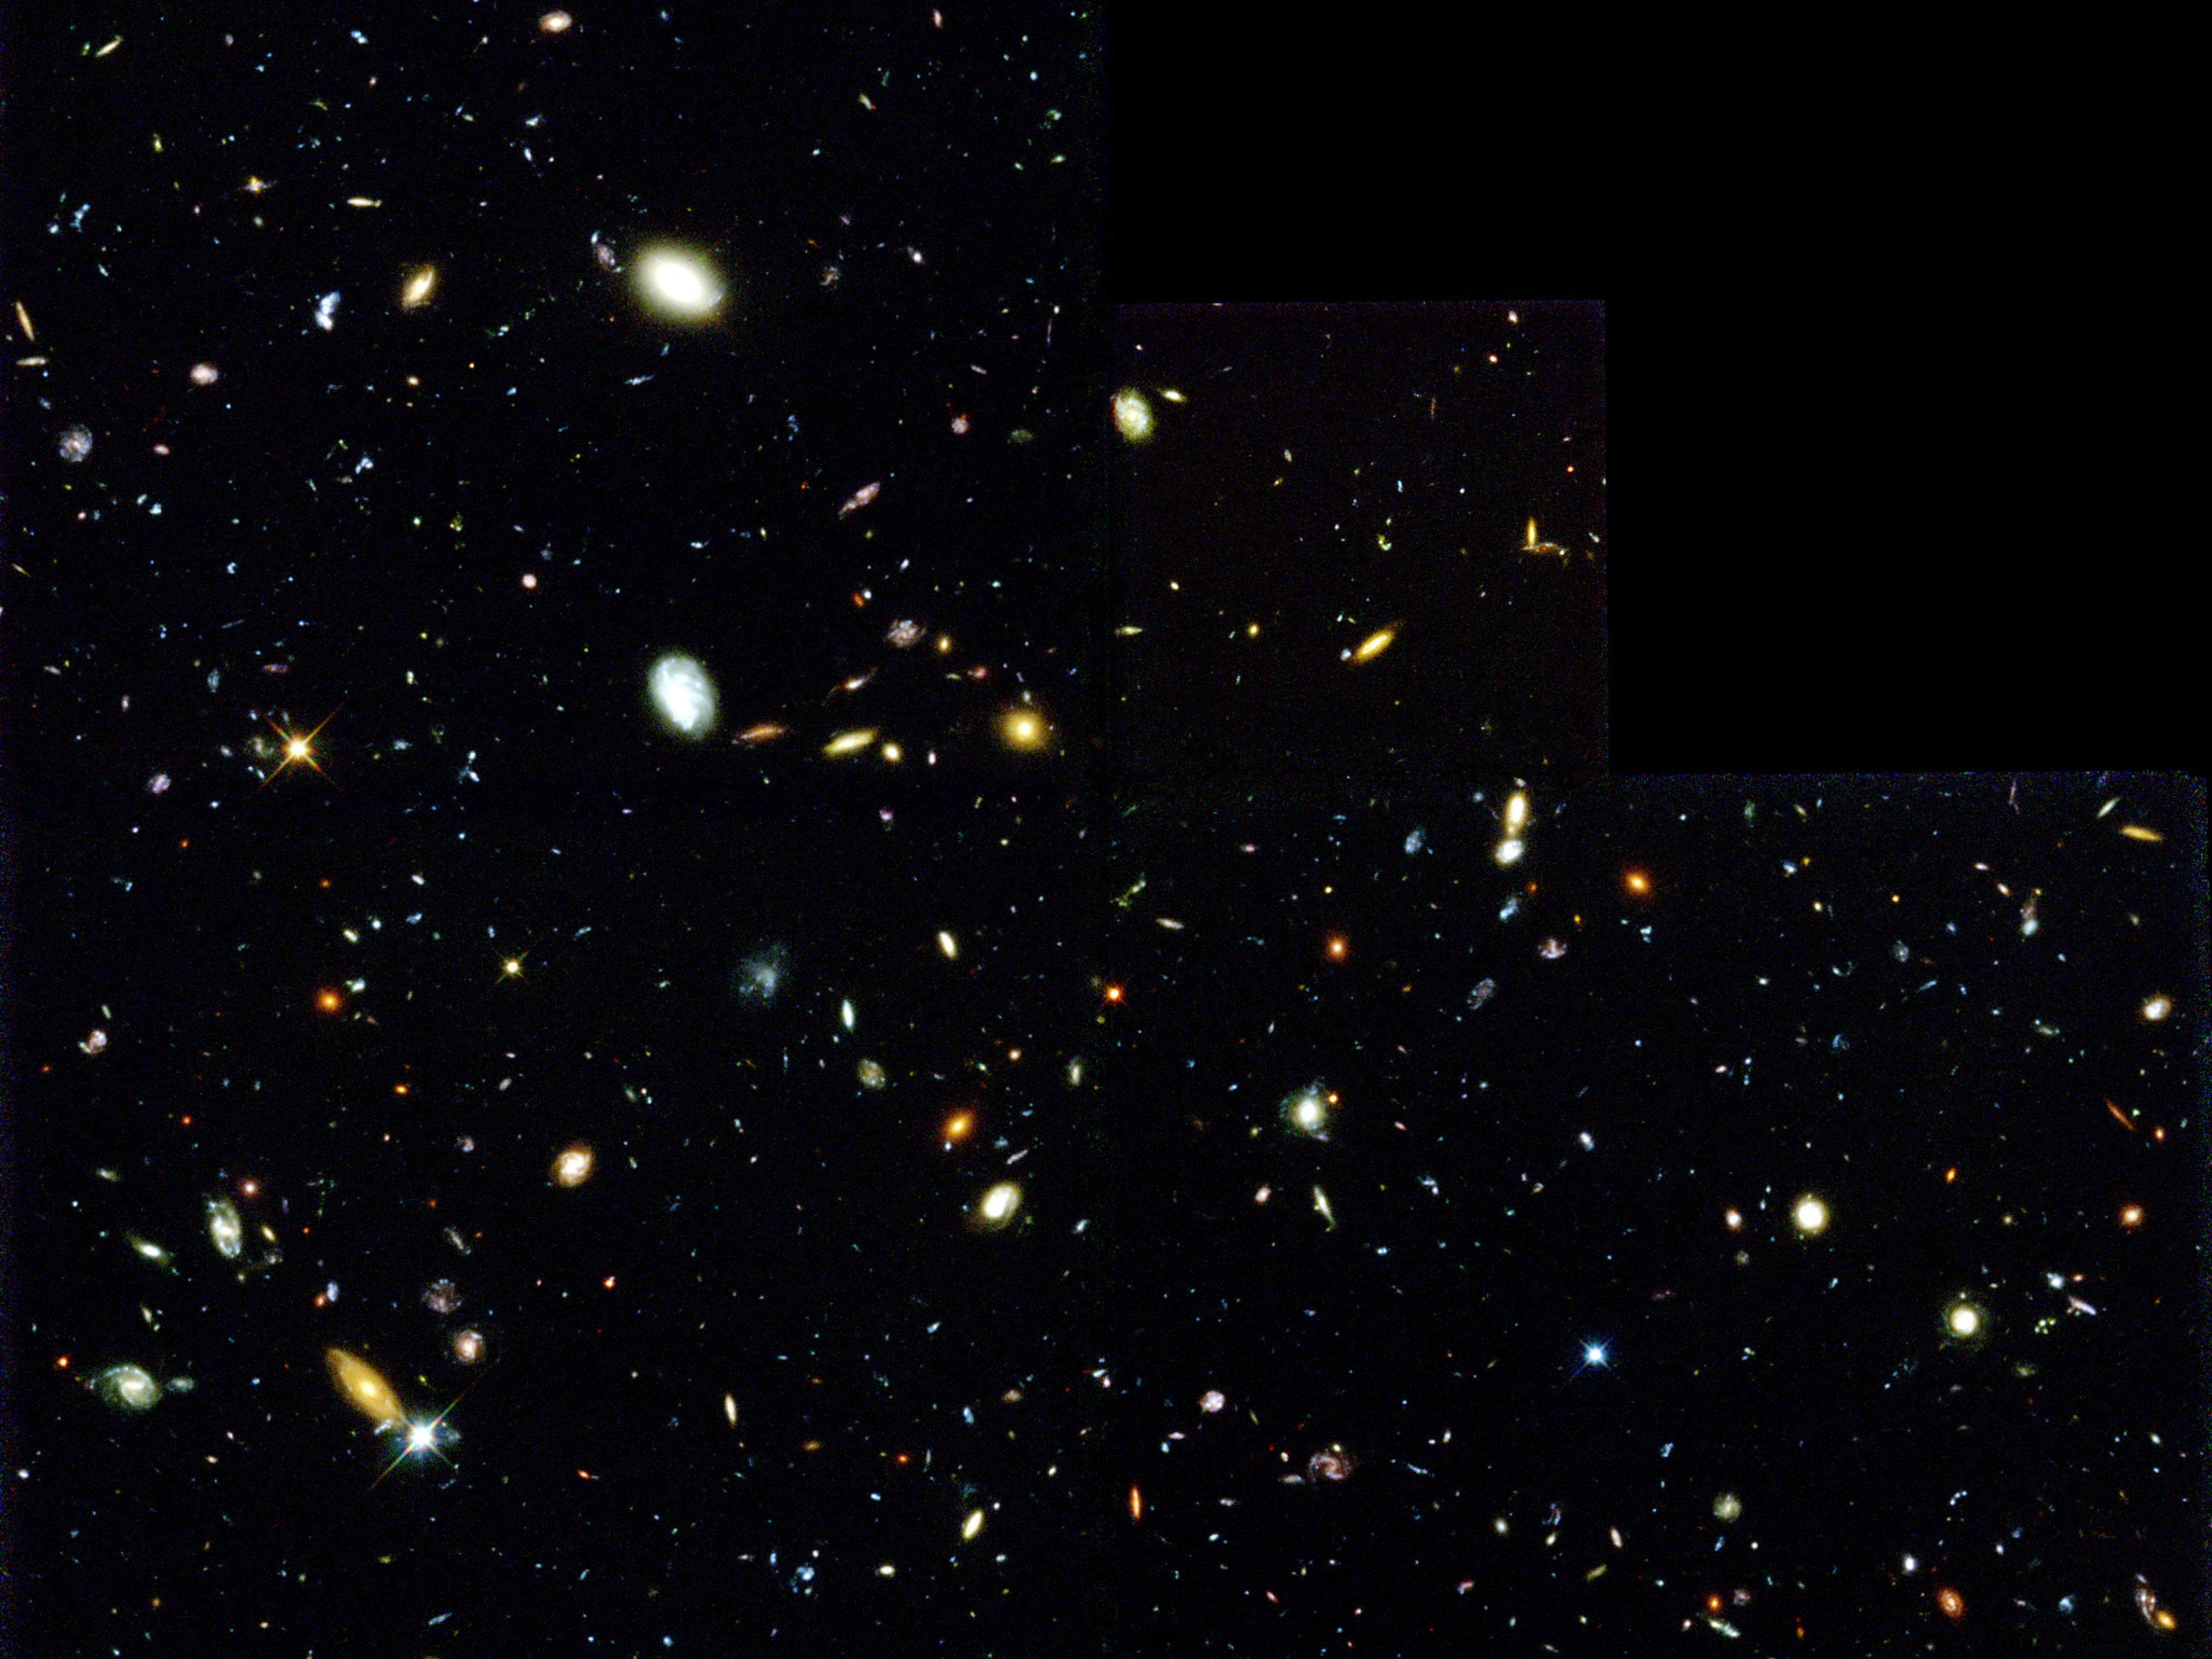
\includegraphics[width=0.9\columnwidth]{Figures/hubble_deep_field.pdf}
	\caption[Hubble Deep Field as captured by the \textit{Hubble Space Telescope}]{The Hubble Deep Field as captured by the Wide Field and Planetary Camera 2 onboard the \textit{Hubble Space Telescope} in 1995 (\citealt{Williams_1996}).}
	\label{fig:hubble_deep_field}
\end{figure}

\section{Galaxy Formation and Evolution}

To answer the questions we have about the evolution of galaxies, we must first make some inferences about the cosmology of the Universe. Our understanding of the cosmic history of galaxies is dependent on our choice of cosmology, which is widely accepted to be the $\Lambda$-CDM model (\citealt{Peebles_1980}). In this cosmology, Cold Dark Matter, matter of unknown origin, dominates over ordinary baryonic matter; and with dark energy, constitute a combined $\sim 95\%$ of the total cosmic energy budget (\citealt{Fukugita_2004}). The presence of dark matter is only evident in its gravitational interactions with matter, but can be inferred from as early as the \textit{surface of last scattering} where it can be seen that the gravitational lensing effect of large-scale distributions of matter led to distortions imprinted in the temperature and density of the cosmic microwave background (CMB). The dark energy in the Universe is parameterized in the form of the cosmological constant, $\Lambda$, which is required to explain the accelerating expansion of the Universe. In this model, galaxy formation is seeded by small quantum fluctuations in the density of the early Universe, which grow with inflation to form small overdensities that later become the sites of dark matter halos by gravitationally attracting nearby dark matter. The first galaxies formed from these originally minute overdensities. Cold dark matter cosmologies favour a \textit{hierarchical model}, where galaxies at later times formed from the coalescence of smaller, gas rich galaxies - leading to a \textit{bottom-up} theory of structure formation. As we shall show in Chapter \ref{chapter:Radio_Identifications}, this model of evolution may not explain the stellar build up of all galaxies.

\subsection{Classification of Galaxies}

The first step in understanding galaxy evolution from direct observations of galaxies across cosmic time, is to classify these galaxies according to their observable properties. Generally, galaxies can be classified into two broad groups based on their morphology: spirals and ellipticals. This dichotomy prompted the first classification scheme by Edwin Hubble (Figure \ref{fig:hubble_tuning_fork}; \citealt{Hubble_1936}), the \textit{Tuning Fork}, which shows elliptical galaxies along the handle, becoming more oblate towards the spiral galaxies. The spiral galaxies themselves are split into two categories forming the two prongs, depending on the presence of a bar at the center. At the join of the two, classified on the \textit{Tuning Fork} as S0, is where we locate \textit{lenticular galaxies}, that are recognized by their large disks, like spirals, but without the presence of arms. In the rest of this Thesis we shall predominantly be referring to elliptical galaxies as \textit{early-type galaxies} (ETGs) and spiral-like galaxies as \textit{late-type galaxies} (LTGs), as is convention. Despite their names, the two do not represent a former and latter evolutionary stage of a typical galaxy, and is rather a misnomer. A minority of galaxies do not conform to this dichotomous image and are typically grouped together as \textit{irregular galaxies}.

\begin{figure}
    \centering
	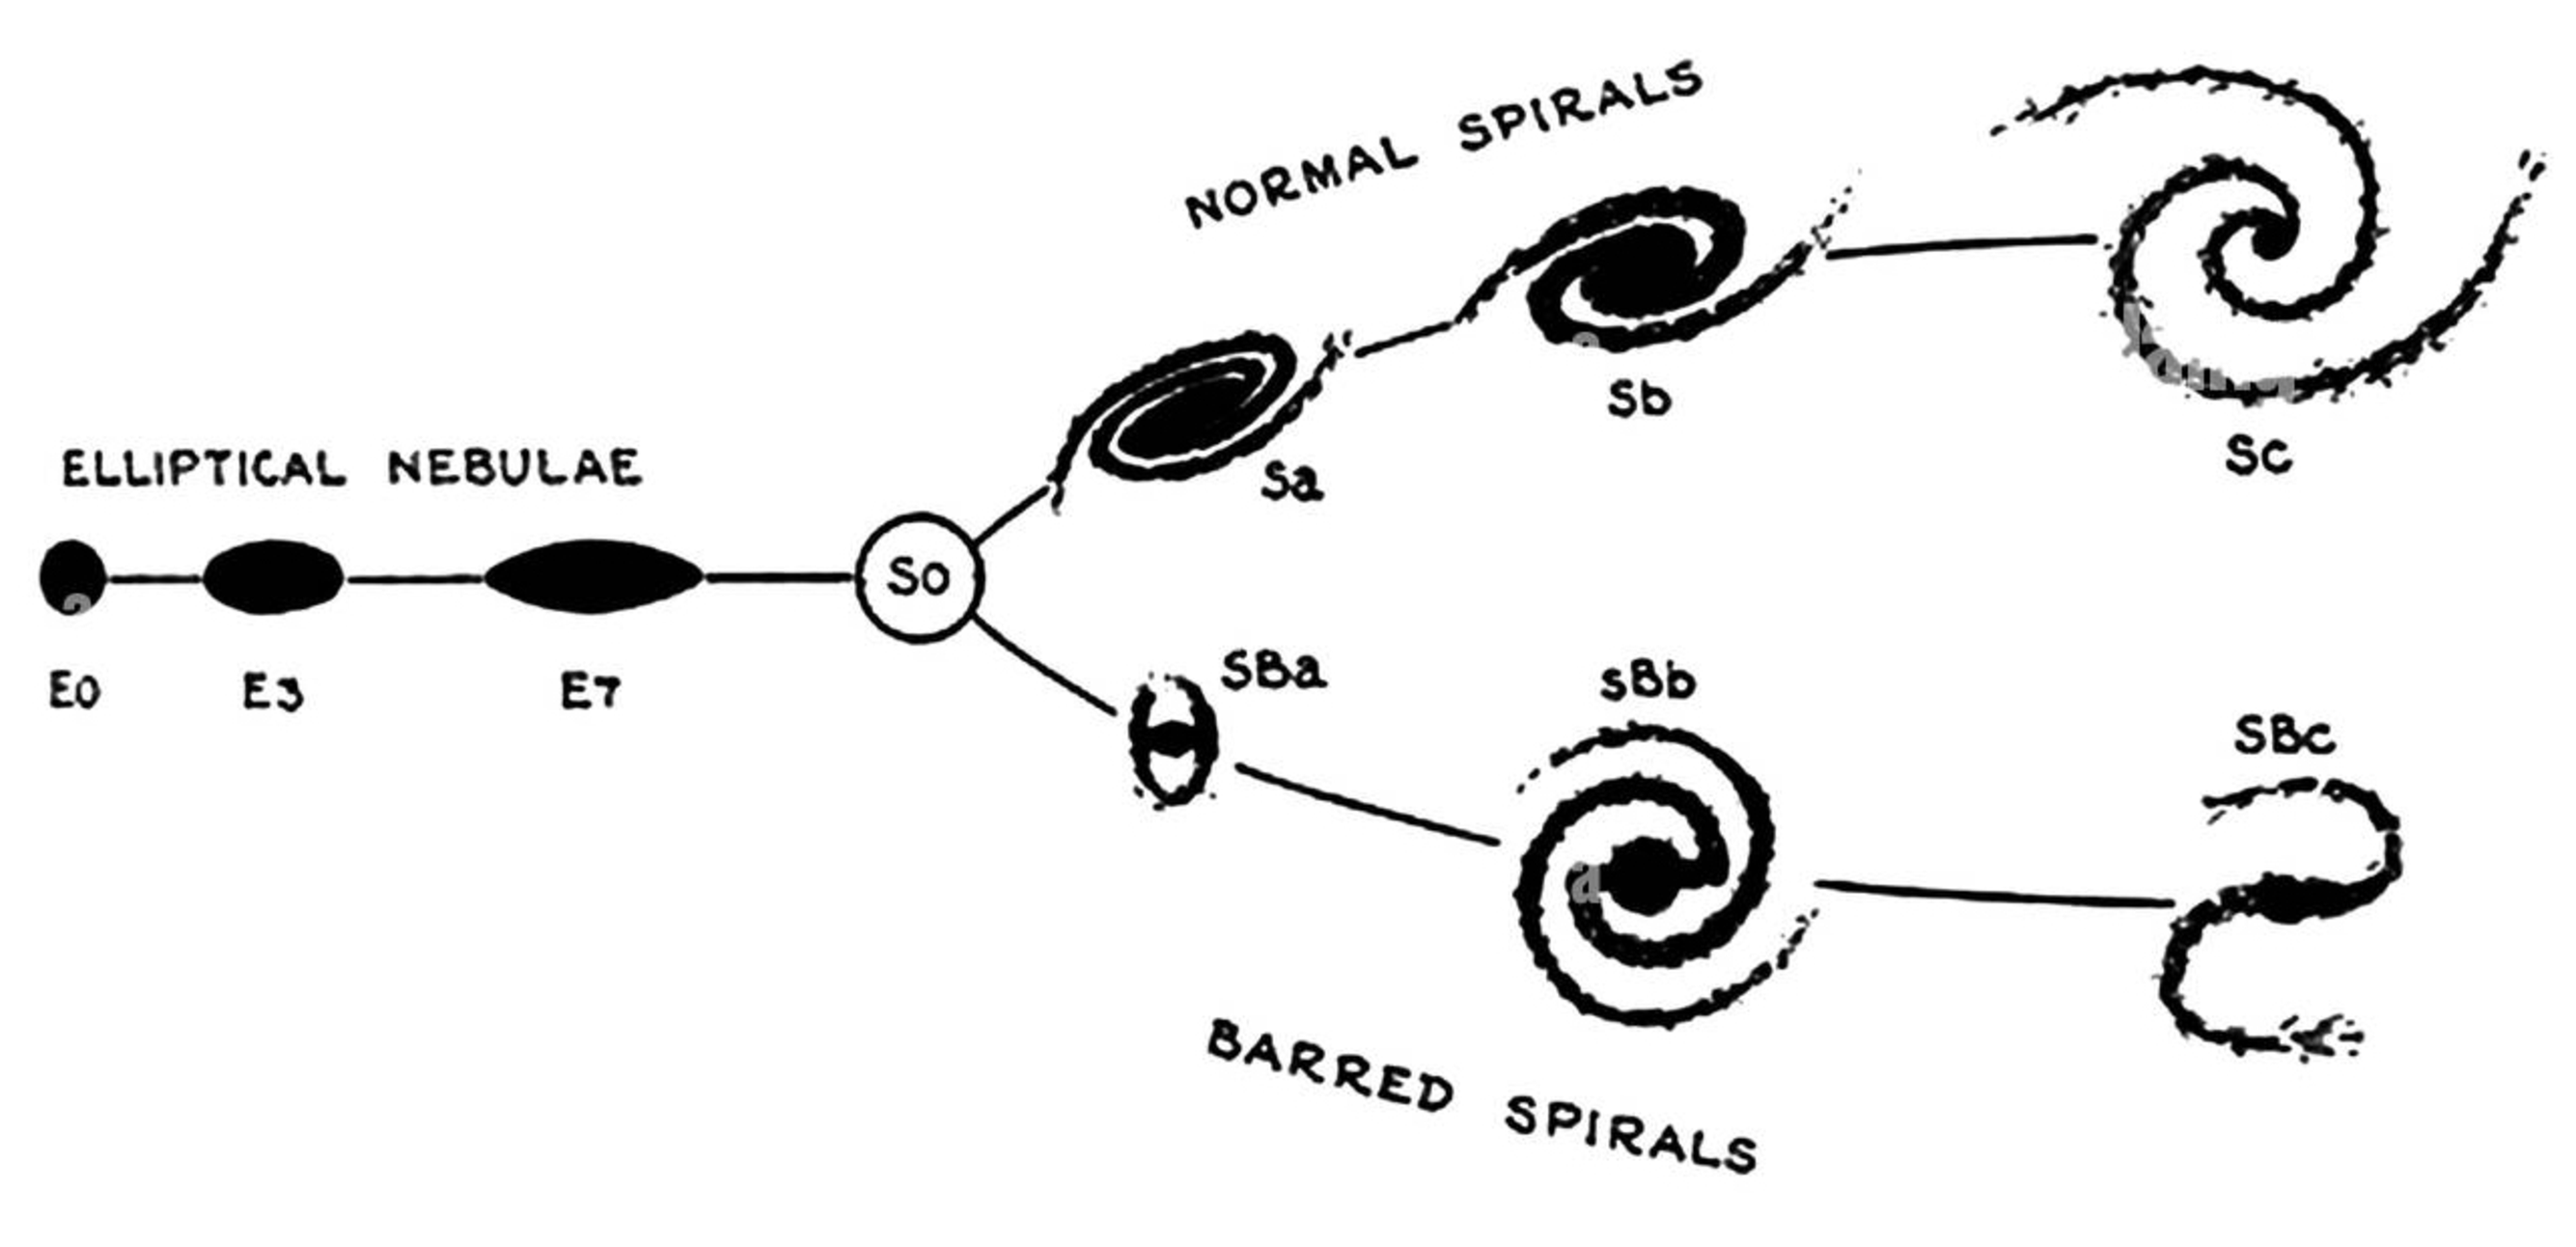
\includegraphics[width=0.9\columnwidth]{Figures/hubble_tuning_fork.pdf}
	\caption[The \textit{Hubble Tuning Fork}]{The \textit{Hubble Tuning Fork}, or the \textit{Sequence of Nebular Types} as named in \citealt{Hubble_1936}, showing spiral galaxies along the prongs of the tuning fork and elliptical galaxies along the handle. The two prongs separate those spiral galaxies with barred central bulges from those that do not. Lenticular galaxies can be found at the join of the handle to the prongs. From left to right, the elliptical galaxies become more oblate and the spiral galaxies have spiral arms that become less tightly wound around the central bulge.}
	\label{fig:hubble_tuning_fork}
\end{figure}

Beyond their shape, the two broad groups, ETGs and LTGs, have a number of physical characteristics that are common to galaxies within each class. First, the stellar populations of ETGs and LTGs are different. ETGs are dominated by old stellar populations that appear red in colour because they contain longer-lived, low mass stars, whereas LTGs typically have younger stellar populations of massive, but very short-lived stars. ETGs are considered to be some of the most massive, luminous galaxies (due to having vast quantities of old stars) observed in the local Universe (\citealt{Bernardi_2003, Kelvin_2014, Moffett_2016}). They are spheroidal in shape with a central bulge of stars where most of the interstellar medium (ISM) is located, though it is not expected to be substantial, and the limited amount of gas in the ISM restricts the level of new star formation. In a hierarchical view of star formation, such ellipticals are formed from a series of major and minor mergers that consume the gas in the galaxy, leading to the quiescent systems observed today (\citealt{Toomre_1972}). In contrast, LTGs have dusty spiral arms with sites of active star formation, with older stars mainly located within the central bulge. While ETGs are largely devoid of gas, LTGs have a rich ISM that continues to fuel star formation, creating new stars at typical rates of a few stars per year (\citealt{Kennicutt_1983, Gao_2004}). Our own Milky Way is an SBc spiral galaxy (\citealt{Gerhard_2002}) with active star formation at a rate of $\sim 2\,M_\odot$yr$^{-1}$ (\citealt{Noriega-Crespo_2013, Licquia_2015, Elia_2022} and references therein).

\subsection{The Star Forming Main Sequence}
\label{sec:star_forming_main_sequence}

A natural diagram to illustrate the difference in the colour of ETGs and LTGs is to plot the colours of optically-selected galaxies against their absolute magnitude. Galaxies discovered in optical surveys readily form two distinct regions: a \textit{red sequence} and a \textit{blue cloud}, with a sparsely populated region in between - the \textit{green valley}. Due to their very different optical colours, the red sequence is dominated by ETGs and the blue cloud dominated by LTGs. Moving away from observed quantities to intrinsic quantities, we note that the colour is a strong indicator of the star formation rate (SFR) in a galaxy and that absolute magnitude is approximately proportional to the size of the stellar population, and thus the stellar mass, $M_*$. In this formalism, the blue galaxies form a tight correlation known as the \textit{Main Sequence} (MS) or \textit{Star Forming Main Sequence}, while the red sequence now occupies a \textit{passive cloud} (or "red and dead" or "quiescent") region that lies below the MS at lower star formation rates (\citealt{Noeske_2007, Daddi_2007, Elbaz_2007, Rodighiero_2011}). Figure \ref{fig:star_forming_main_sequence} shows the local main sequence and passive cloud (grey contours) that form from optically-selected Sloan Digital Sky Survey (SDSS; \citealt{York_2000}) galaxies in the redshift interval $0.01 < z < 0.05$. Additionally, \citealt{Saintonge_2017} present the \textit{Extended CO Legacy Database for GASS}, xCOLD GASS, a mass-selected sample from SDSS that have molecular gas mass estimates, which are overplotted in colour. The molecular gas mass fraction, $f_{\textrm{H}_2} \equiv M_{\textrm{H}_2}/M_*$, clearly declines towards the passive cloud, showing the depleted amount of gas in ETGs.

\begin{figure}
    \centering
	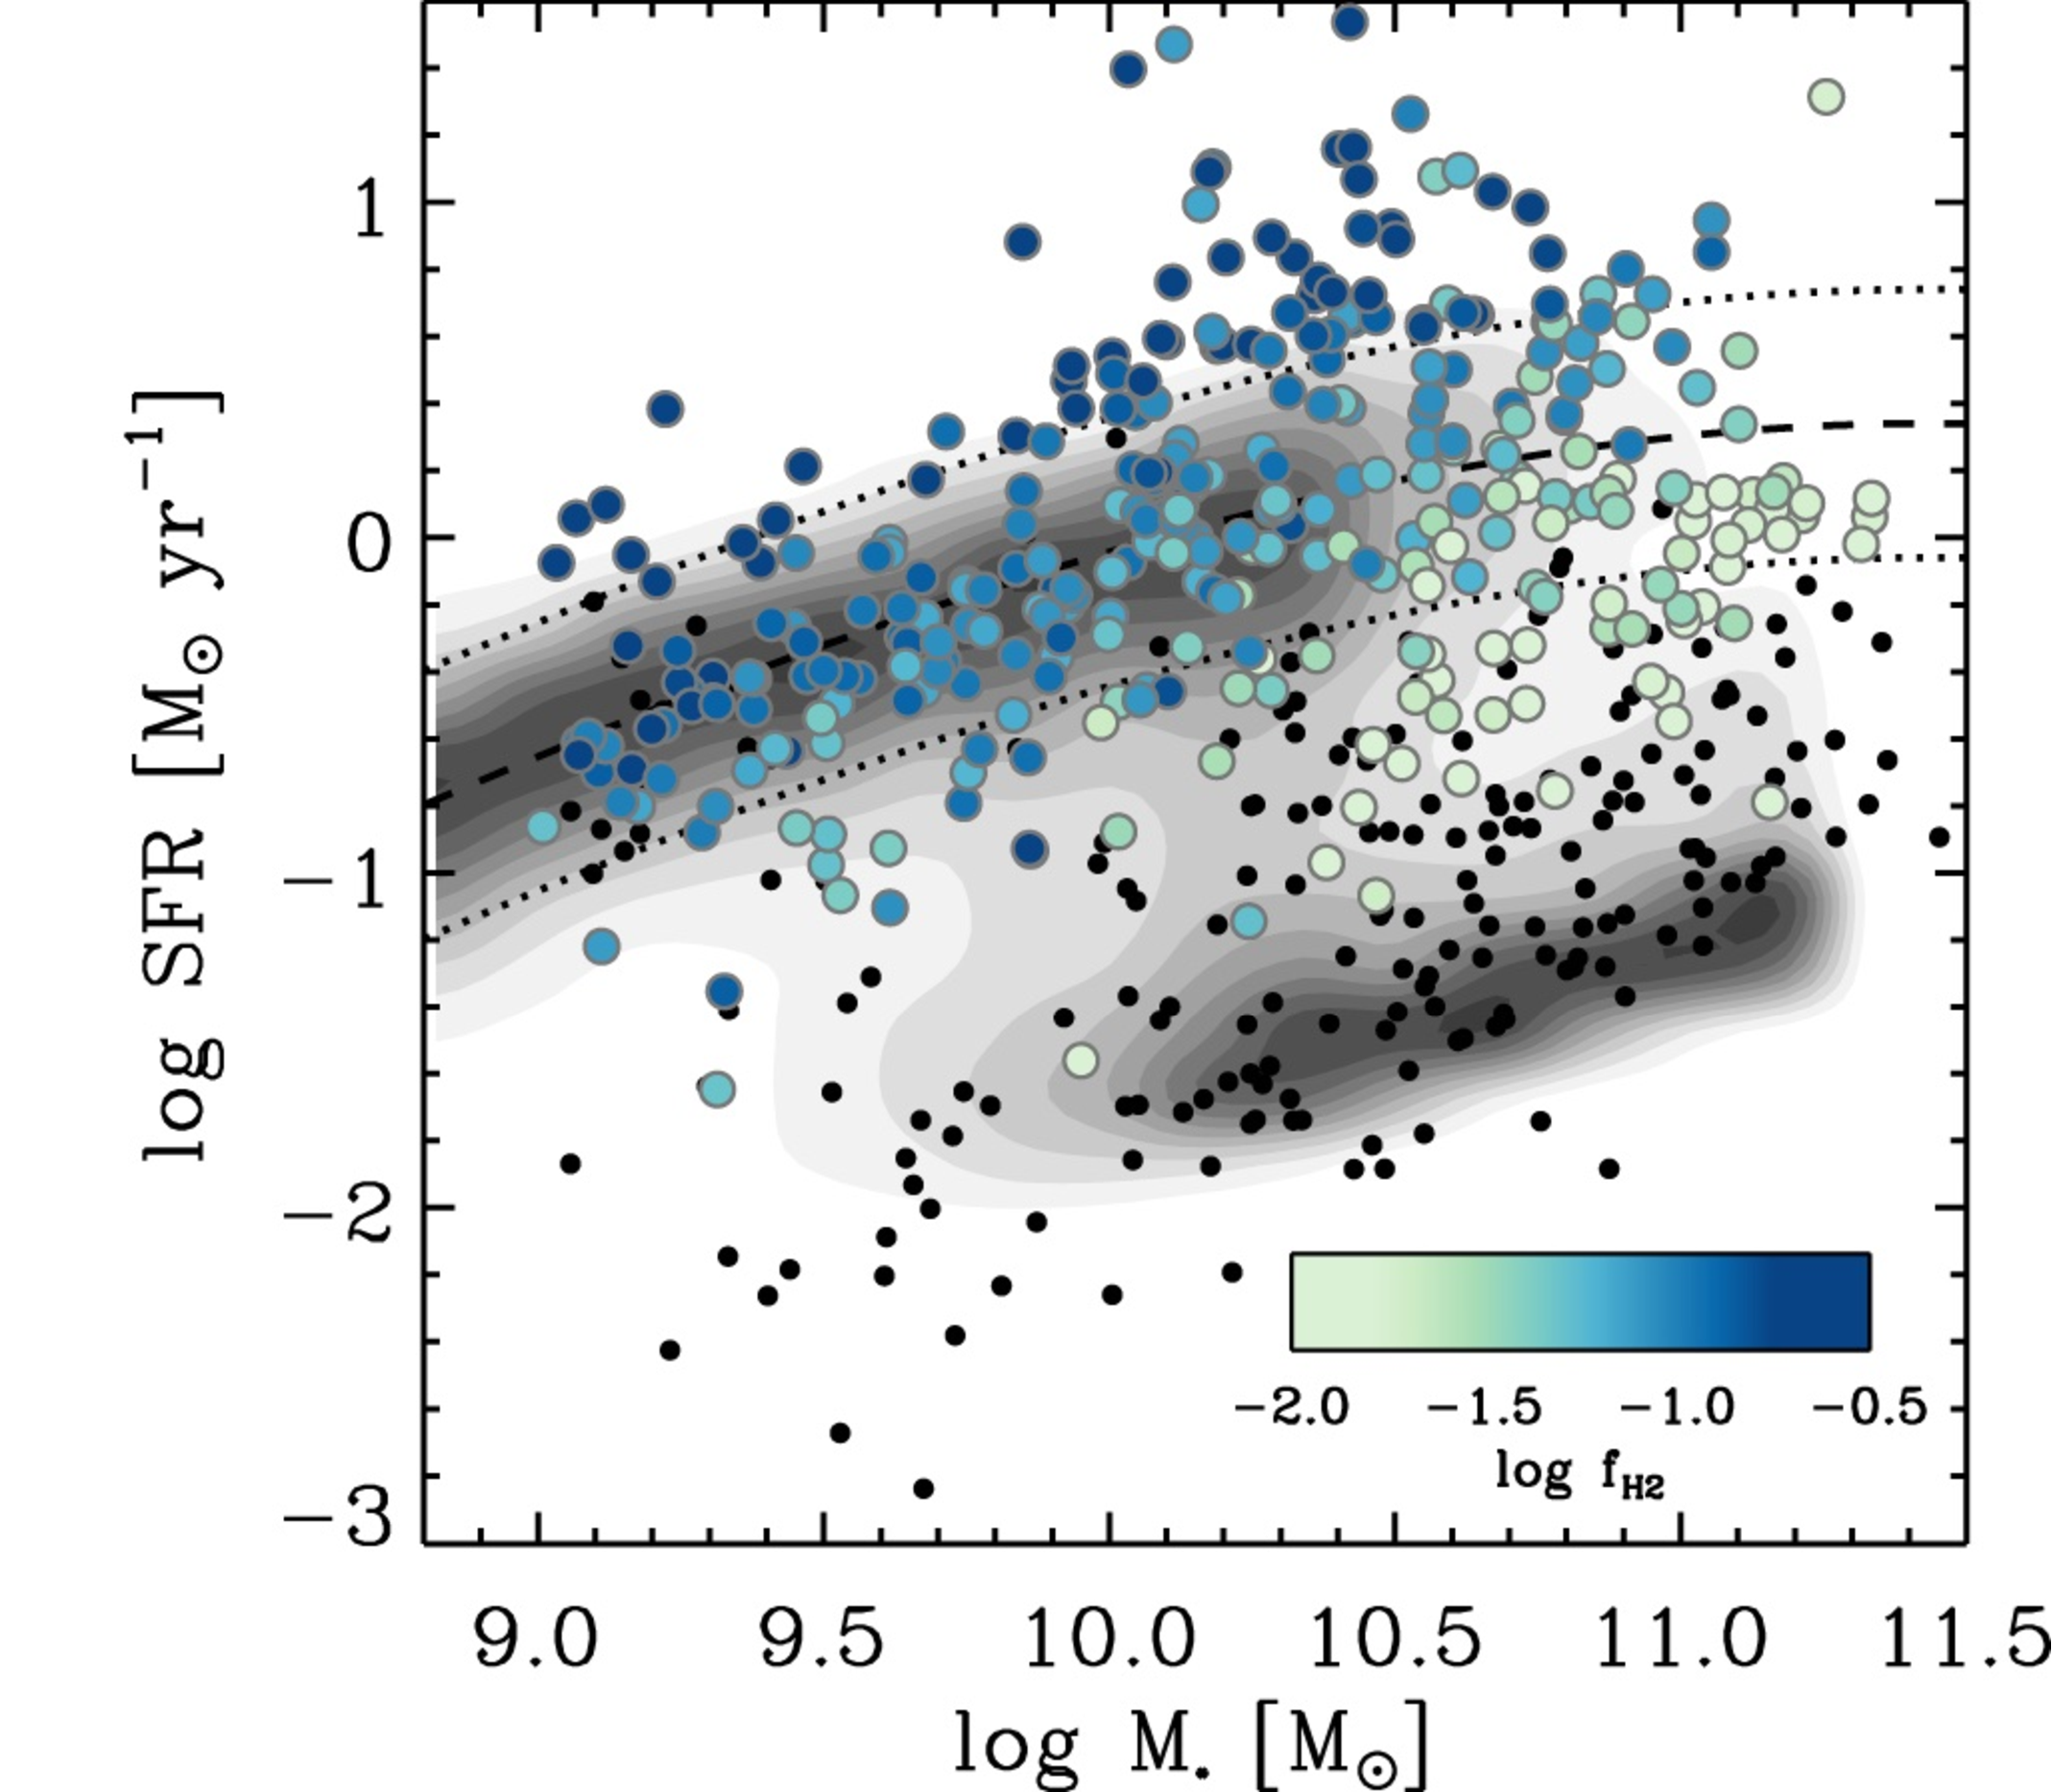
\includegraphics[width=0.8\columnwidth]{Figures/saintonge_ms.pdf}
	\caption[The distribution of SDSS galaxies in the SFR-$M_*$ plane]{The distribution of SDSS galaxies in the SFR-$M_*$ plane (grey contours) from \citealt{Saintonge_2017} (Figure 8). The dashed line represents the location of the main sequence, while the dotted lines represent $\pm0.4\,$dex scatter around this relationship. The coloured points show the distribution of galaxies from xCOLD GASS, coloured according to their molecular gas mass fraction. The black points are galaxies without detected CO (1 - 0) emission lines, as used to measure the mass of molecular gas.}
	\label{fig:star_forming_main_sequence}
\end{figure}

It is predicted that the vast majority, approximately $90\%$, of all cosmic star formation between redshifts $0$ and $2.5$ occurs in galaxies that reside on the MS (\citealt{Rodighiero_2011, Sargent_2012}), however, we also know that an important contribution comes from galaxies that sit substantially above this relation. These galaxies, undergoing high levels of star formation for a short period of time, are collectively referred to as \textit{starburst galaxies} (e.g. \citealt{Muxlow_2006, Rinaldi_2022}). Starbursts\footnote{Unfortunately, there is yet to be a population of galaxies referred to as \textit{Opal Fruits}.} form a small minority of galaxies, approximately $2\%$ of star forming galaxies depending on the exact definition of a starburst, but contribute $\sim 10\%$ of the cosmic star formation rate density (SFRD) at $z \sim 2$ (\citealt{Rodighiero_2011}), corresponding to the time in cosmic history when star formation was at its peak (see Section \ref{sec:cosmic_star_formation_history}).

Given that galaxies in the passive cloud have large stellar masses, they must have been at some point among the actively star forming galaxies, following which some process quenched them of their star formation leading them to the passive cloud. There are many possibilities that have been proposed as the cause of quenching, and it is likely that all are important in some regard. These processes include, but may not be limited to: stellar feedback and winds from supernovae removing the gas from a galaxy (\citealt{Hayward_2017}); gas expulsion by active galactic nuclei (AGN; \citealt{Springel_2005, Croton_2006, Cicone_2014, Harrison_2017}); the formation of a galactic bar or central bulge (\citealt{Bournaud_2007, Martig_2009}) which relocates the gas to the galactic center and reduces the star formation in the disk; a range of environmental processes such as galaxy merging (\citealt{Lavery_1994, Weigel_2017}) which ignites a starbursting phase that rapidly consumes the gas; ram-pressure stripping, the loss of gas as the galaxy passes through the intra-cluster medium (\citealt{Gunn_1972, Boselli_2006, Domainko_2006, Boselli_2014}), and quenching mechanisms that result from being in high density environments, like galaxy harassment and strangulation (\citealt{Moore_1996, Moore_1998, Bekki_2002}). While we do not have a clear understanding of which mechanisms play the most important roles in quenching star formation, different processes have been proposed based on the mass of the galaxy. In general, massive galaxies are more likely quenched by internal processes and less affected by the environment in which they reside, while smaller galaxies are more likely quenched by processes that are independent of their stellar mass, particularly if they sit within dense environments (\citealt{Contini_2019}). At low masses ($\lesssim 10^9\,M_\odot$), gas outflows from stellar winds and supernovae are expected to drive the quenching of star formation (\citealt{Dekel_1986, DallaVecchia_2008}), and at higher masses ($\gtrsim 10^{10}\,M_\odot$), quenching either by heating of cold gas from radio jets, or from gas expelled by outflows of an AGN are more effective (\citealt{Croton_2006, Fabian_2012, Fang_2013, Cicone_2014}).

\subsection{Cosmic Star Formation History}
\label{sec:cosmic_star_formation_history}

We have seen that the star formation rates of galaxies are intrinsically linked to their evolutionary stage, and thus it is unsurprising that we identify an evolution in the integrated SFRs of galaxies with cosmic time. By measuring the star formation of many galaxies at different epochs, we can build a picture of the star formation density in the Universe. The cosmic history of star formation is one of the fundamental observables of astronomy, giving us an insight into the timeline for which gas forms into stars, heavy elements are produced (elements heavier than the primordial hydrogen and helium are produced in stars), and dust is formed (as dust is a natural byproduct of star formation, see Section \ref{sec:lifecycle_of_dust}).

The cosmic star formation rate density in the Universe is straightforwardly estimated from the star formation rates of galaxies based on their rest frame UV photometry. The UV maps the light from hot, young, massive stars and therefore directly traces recent star formation (e.g. \citealt{Madau_1996, Lilly_1996, Wyder_2005, Schiminovich_2005, Dahlen_2007, Reddy_2009, Robotham_2011, Cucciati_2012, Schenker_2013, Finkelstein_2015}). However, we also note that approximately half of all optical and UV light from stars ever emitted in the Universe has been absorbed by dust and re-emitted at far-infrared (FIR) and sub-millimeter (sub-mm) wavelengths (\citealt{Puget_1996, Fixsen_1998, Dole_2006, Driver_2008, Driver_2016}). This means that a significant contribution to the SFRD is hidden behind dust and must be determined from far-IR/sub-mm indicators of star formation that probe the reprocessed stellar light (e.g. \citealt{Magnelli_2011, Casey_2012, Magnelli_2013, Gruppioni_2013, Swinbank_2014, Bouwens_2016, Bourne_2017, Koprowski_2017, Novak_2017, Liu_2018, Bouwens_2020, Dudzeviciute_2020}).

Figure \ref{fig:cosmic_sfrd} shows that the dust-obscured and unobscured measures of the SFRD have peaks at $z\sim2$ (when the Universe was roughly $3$ billion years old), followed by a slow decline by a factor of $\sim 8$ to the present day. The short period corresponding to the peak of star formation is often referred to as \textit{cosmic noon}. In the approximate $3.5\,$Gyr between $z\sim3$ and $z\sim1$, spanning cosmic noon, up to half of the stellar mass we observe today was formed (\citealt{Forster-Schreiber_2020}). The galaxies that are identified at these redshifts are ideal targets for tracing the formational epoch of the massive LTGs and ETGs seen in the local Universe. We see that most of the star formation at $z < 3$ is obscured by dust and even at higher redshifts the contribution still appears significant. The FIR and sub-mm traced component has dominated the cosmic history of star formation for the past $\sim 12\,$Gyr, contributing approximately $80\%$ of the total star formation. The top panel of Figure \ref{fig:cosmic_sfrd} shows the contribution from galaxies with different IR luminosities to the dust-obscured star formation rate density. It is clear that, of the IR luminous galaxies, it is the massive, most luminous galaxies that dominate the dust-obscured star formation history at earlier times. It is such galaxies, that appear particularly bright at far-IR wavelengths, that are crucial for our understanding of obscured star formation. First, we clarify some acronyms commonly used to refer to bright infrared galaxies that will be referred to throughout the Thesis (the IR luminosities of galaxies are assumed to be the bolometric luminosity integrated between $8$ and $1,000\,\mu$m in the rest frame):

\begin{itemize}
    \item Luminous Infrared Galaxy (LIRG: $10^{11} < L_\textrm{IR} [L_\odot] < 10^{12}$).
    \item UltraLuminous Infrared Galaxy (ULIRG: $10^{12} < L_\textrm{IR} [L_\odot] < 10^{13}$).
    \item HyperLuminous Infrared Galaxy (HyLIRG: $L_\textrm{IR} [L_\odot] > 10^{13}$).
\end{itemize}

\begin{figure}
    \centering
	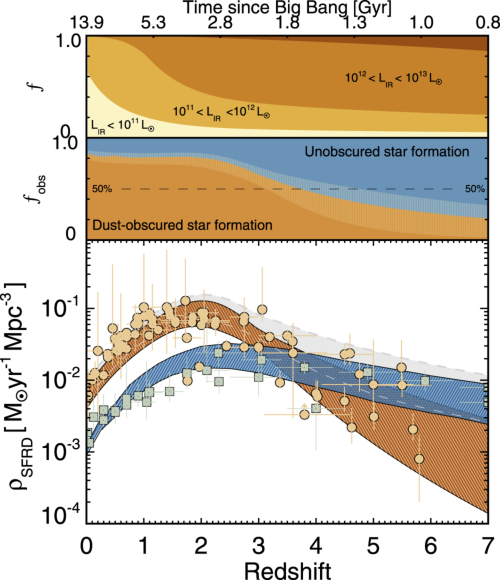
\includegraphics[width=0.8\columnwidth]{Figures/cosmic_sfrd.pdf}
	\caption[Cosmic star formation history]{The cosmic star formation history from \citealt{Zavala_2021}. Contributions to the total star formation rate density (grey) from dust-obscured IR/sub-mm surveys and from unobscured UV/optical surveys are shown in orange and blue, respectively. The top panel shows the relative contribution to the dust-obscured SFRD from galaxies with different IR luminosities. The middle panel represents the fraction of SFRD that is dust-obscured.}
	\label{fig:cosmic_sfrd}
\end{figure}

Looking back to cosmic noon, much of the star formation within dusty galaxies is happening in ULIRGs, while the integrated dust-obscured star formation begins to fall. This suggests that the number of massive galaxies declines at higher redshifts, but their individual contribution becomes more important. Particularly at high redshifts ($z \gtrsim 3$), the exact amount of dust-obscured star formation is still uncertain and large samples of galaxies with measured dust emission are required to elucidate our view on the cosmic history of star formation.

\section{The Interstellar Medium}

The interstellar medium (ISM) refers to the matter that fills the space in between the stars of a galaxy. It is the medium in which stars are born, and latter replenished with enriched material when they die. The baryonic matter comes in the form of gas - in ionic, atomic and molecular forms - and dust, in overwhelming favour of gas which constitutes $\sim99\%$ of the ISM, and dust the other $1\%$ (\citealt{Ferriere_2001}). By mass, the gas in the ISM is around $70\%$ hydrogen, $28\%$ helium and $2\%$ heavier elements, reflecting only a small change from the ratios of the primordial matter created after the Big Bang (\citealt{Klessen_2016}). In terms of volume, most of the ISM is occupied by ionized gas, but due to its incredibly low volume density, only accounts for around $25\%$ of the gas mass. Most of the gas mass in a galaxy is in the form of neutral atomic gas (H and He) or molecular gas (H$_2$) found in dense clouds that take up only $1 - 2\%$ of the total volume of the ISM (\citealt{Dyson_1997, Klessen_2016}).

The ISM spans a wide range of temperatures and densities, leading to many models of the ISM being in distinct phases, despite there being no obvious separation between them (\citealt{Cox_2005}). A two phase model was first proposed by \citealt{Field_1969}, showing that atomic gas in the ISM can exist at two stable temperatures. These two solutions correspond to cold and dense gas at $T\sim100\,$K and warm, diffuse gas at $T\sim10^4\,$K. These are now referred to as the Cold Neutral Medium (CNM) and Warm Neutral Medium (WNM), respectively. This model was extended to three phases by \citealt{McKee_1977}, who noted that supernovae in the ISM creates bubbles of very hot, ionized gas ($T\sim10^6\,$K); this phase of the ISM is known as the Hot Ionized Medium (HIM). However, $90\%$ of the ionized gas in the ISM is to be found in a cooler, Warm Ionized Medium (WIM) where ionizing photons are produced by rare, massive stars (\citealt{Haffner_2009}). A final distinction is typically made for the molecular clouds that are cold, but distinctly more dense than the CNM. These molecular gas clouds have a range of masses and sizes, and their location are known to correlate with observed star formation in the Galaxy. The approximate temperatures, densities, mass fractions and volume filling fractions of each phase in the ISM for a dynamic spiral galaxy are given in Table \ref{tab:ISM_phases}. The fractions are highly uncertain but represent what might be realistic estimates for a spiral galaxy containing all five phases of this interpretation of the ISM. This multi-phase picture is certainly an oversimplification of the conditions found in the ISM. The ISM is shaped by a variety of processes that blur the distinction between these phases, such as turbulence from supernova shocks (\citealt{MacLow_2004}) and stellar winds, thermal instability (\citealt{Kritsuk_2002}) and the presence of magnetic fields. The actual ISM in a galaxy is continuous and dynamic with transitional regions.

\begin{table}
	\centering
	\begin{tabular}{p{4cm}|p{2.5cm}|p{2.75cm}|p{1.5cm}|p{2cm}}
		\hline
		\hline
		Phase & T [K] & $n$ [atoms cm$^{-3}$] & $f_{\textrm{Mass}}$ & $f_{\textrm{Volume}}$ \\
		\hline
		\hline
		Molecular Clouds & $10 - 20$ & $>10^2$ & $\sim 20\%$ & $<1\%$ \\
		Cold Neutral Medium & $50 - 100$ & $20 - 50$ & $\sim 40\%$ & $\sim2 - 4 \%$\\
		Warm Neutral Medium & $(6 - 10)\times10^3$ & $0.2 - 0.5$ & $\sim 30\%$ & $\gtrsim 30\%$ \\
		Warm Ionized Medium & $\sim8\times10^3$ & $0.2 - 0.5$ & $\sim 10\%$ & $\gtrsim 15\%$ \\
		Hot Ionized Medium & $\sim10^6$ & $\sim10^{-2}$ & $\sim 1\%$ & $\lesssim 50\%$ \\
		\hline
	\end{tabular}
	\caption[The temperatures, densities, mass and volume filling factors of ISM phases]{The different phases of the ISM and their expected temperatures, densities, mass fractions and volume filling factors, as tabulated in \citealt{Ferriere_2001}.}
	\label{tab:ISM_phases}
\end{table}

Figure \ref{fig:interstellar_medium} shows various components of the ISM in the Galaxy, as traced by different wavelengths of the electromagnetic spectrum. The top two panels highlight the starlight that is observable at optical ($0.5\,\mu$m) and near-infrared ($2\,\mu$m) wavelengths. The stellar light is blocked by dust in the optical image, whereas the near-infrared clearly shows the stellar distribution, making the dark dust clouds appear almost transparent. The benefit that the infrared provides in identifying the stellar light of a galaxy, compared to optical wavelengths, is a key motive for the studies presented in Chapters \ref{chapter:Data_Release_3} and \ref{chapter:Dust_Mass_Functions}. As we traverse the electromagnetic spectrum to the thermal peak in the far-infrared (third panel, observed at $350\,\mu$m) the emission from the dust itself becomes visible. The final three panels show the emission from atomic, ionized and molecular gas in the Galaxy. The atomic gas is traced by the $21\,$cm spectral line, originating from the hydrogen \textit{spin-flip} transition between a proton-electron aligned state to an anti-aligned state. This transition is forbidden - the mean lifetime of a hydrogen atom being in the excited, aligned state is approximately $11$ million years (\citealt{Mhaske_2022}) - meaning that the likelihood of the transition is incredibly rare. However, as can be seen in the figure, the abundance of atomic hydrogen means that the $21\,$cm line is still a useful tracer for gas in the ISM. The limitation of the $21\,$cm line is that it is only useful for tracing the distribution of neutral hydrogen in the local Universe where the emission is strong enough to be detected. The $74\,$cm radio emission in the penultimate panel traces the radiation from ionized gas. The radio emission emanates from accelerated charged particles, which may be observed in HII regions and supernova remnants. The final panel shows the molecular gas phase, as traced by the $2.6\,$mm spectral line of carbon monoxide (CO). As will be detailed later, the rotational transitions of the CO molecule are a useful tracer of dense molecular regions. This map therefore shows the locations of cold gas in the Galaxy and the sites of star formation.

\begin{figure}
    \centering
	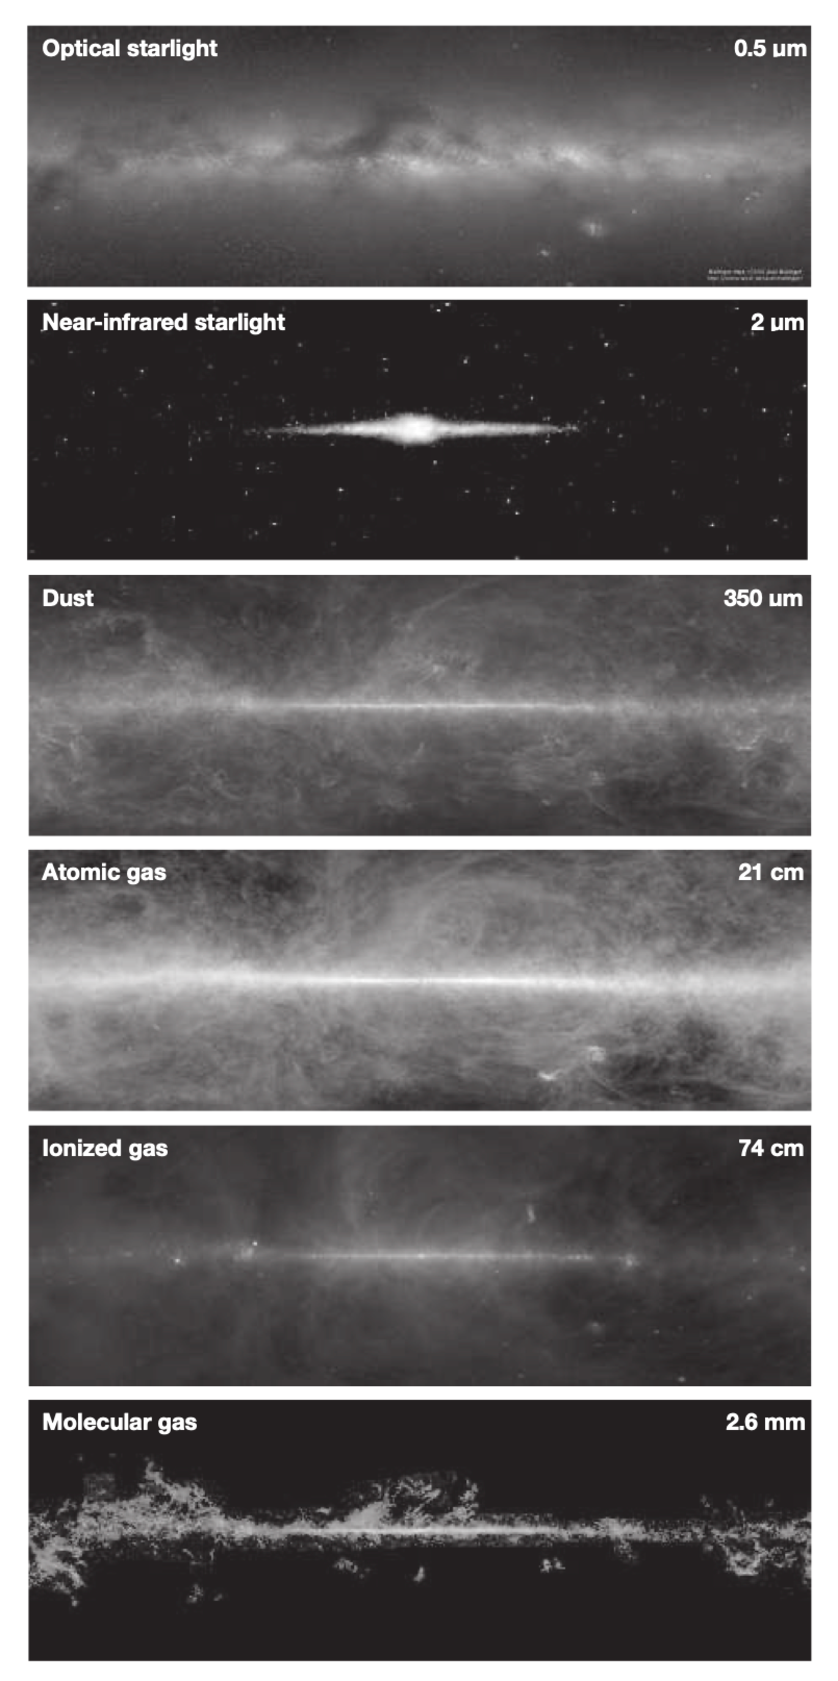
\includegraphics[width=0.75\columnwidth, height=0.92\textheight]{Figures/interstellar_medium.pdf}
	\caption[The plane of the Galaxy observed at various wavelengths]{The plane of the Galaxy observed at different wavelengths as presented in \citealt{Williams_2021}. From top to bottom the panels show: the optical starlight at $0.5\,\mu$m; the near-infrared starlight at $2\,\mu$m; the interstellar dust at $350\,\mu$m; the atomic gas at $21\,$cm; the ionized gas at $74\,$cm and the molecular gas at $2.6\,$mm.}
	\label{fig:interstellar_medium}
\end{figure}

\section{Cosmic Dust}

\subsection{Chemical Composition of Dust}

Cosmic dust is a general term that refers to the solid particles that exist in the ISM. These interstellar grains can have a range of sizes between $\sim 10\,$nm and $\sim 1\,\mu$m (\citealt{Kim_1994, Galliano_2018}) and are mostly composed of carbonaceous materials (materials that are predominantly carbon by mass) and silicates. The larger dust grains are primarily silicates and amorphous carbon, which are prime candidates for the dust grains that absorb UV and optical starlight and reradiates this energy in the far-IR and sub-mm regimes. Hydrogenated carbonaceous materials, like Polycyclic Aromatic Hydrocarbons (PAHs), are chemical compounds formed of carbon and hydrogen molecules and are also an important component of interstellar dust grains. These molecules are the cause of strong spectral lines that can be observed in the mid-infrared (\citealt{Tielens_1987, Draine_2007a, Draine_2007b}).

\subsection{The Reprocessing of Starlight}

The presence of dust along the line of sight to a population of stars can have several effects on the emission that is observed. First, if the dust is thick enough, any background stellar light may not be visible at all, as is the case with some dark nebulae in the Galaxy such as the \textit{Horsehead Nebula} (\citealt{Greenberg_2002}). For less opaque dust clouds, the light passing through can be dimmed due to the effects of dust extinction. This refers to the amount of background light that is absorbed and scattered out of the line of sight to the observer. The dimming effect is dependent on several factors including the density of the dust cloud, the grain size distribution and the wavelength of the light. More generally, dust attenuation refers to the combined effects of dust on the spectrum of a background object, including dust extinction, but also includes scattering back into the line of sight and the light from unobscured stars. It is the attenuated stellar emission that is observed as a strong peak in the far-IR region of a galaxy's spectral energy distribution (SED). Figure \ref{fig:unattenuated_attenuated_sed} shows the UV to far-IR SED of NGC 337, modelled using \texttt{MAGPHYS} (\citealt{daCunha_2008}), which illustrates how the true stellar spectrum of a galaxy (blue) is attenuated by dust to produce the far-IR emission (green) and the observed UV to far-IR spectrum (black). Moreover, interstellar dust is more efficient at absorbing and scattering blue light compared to red light, due to its shorter wavelength corresponding to the typical size of abundant small grains, meaning that background stars behind a cloud of dust often appear more red than they really are. This effect is known as dust reddening and can be observed in the spectrum of NGC 337 - the shorter the wavelength (towards the blue end of the spectrum), the greater the difference between the attenuated and unattenuated stellar spectra.

\begin{figure}
    \centering
	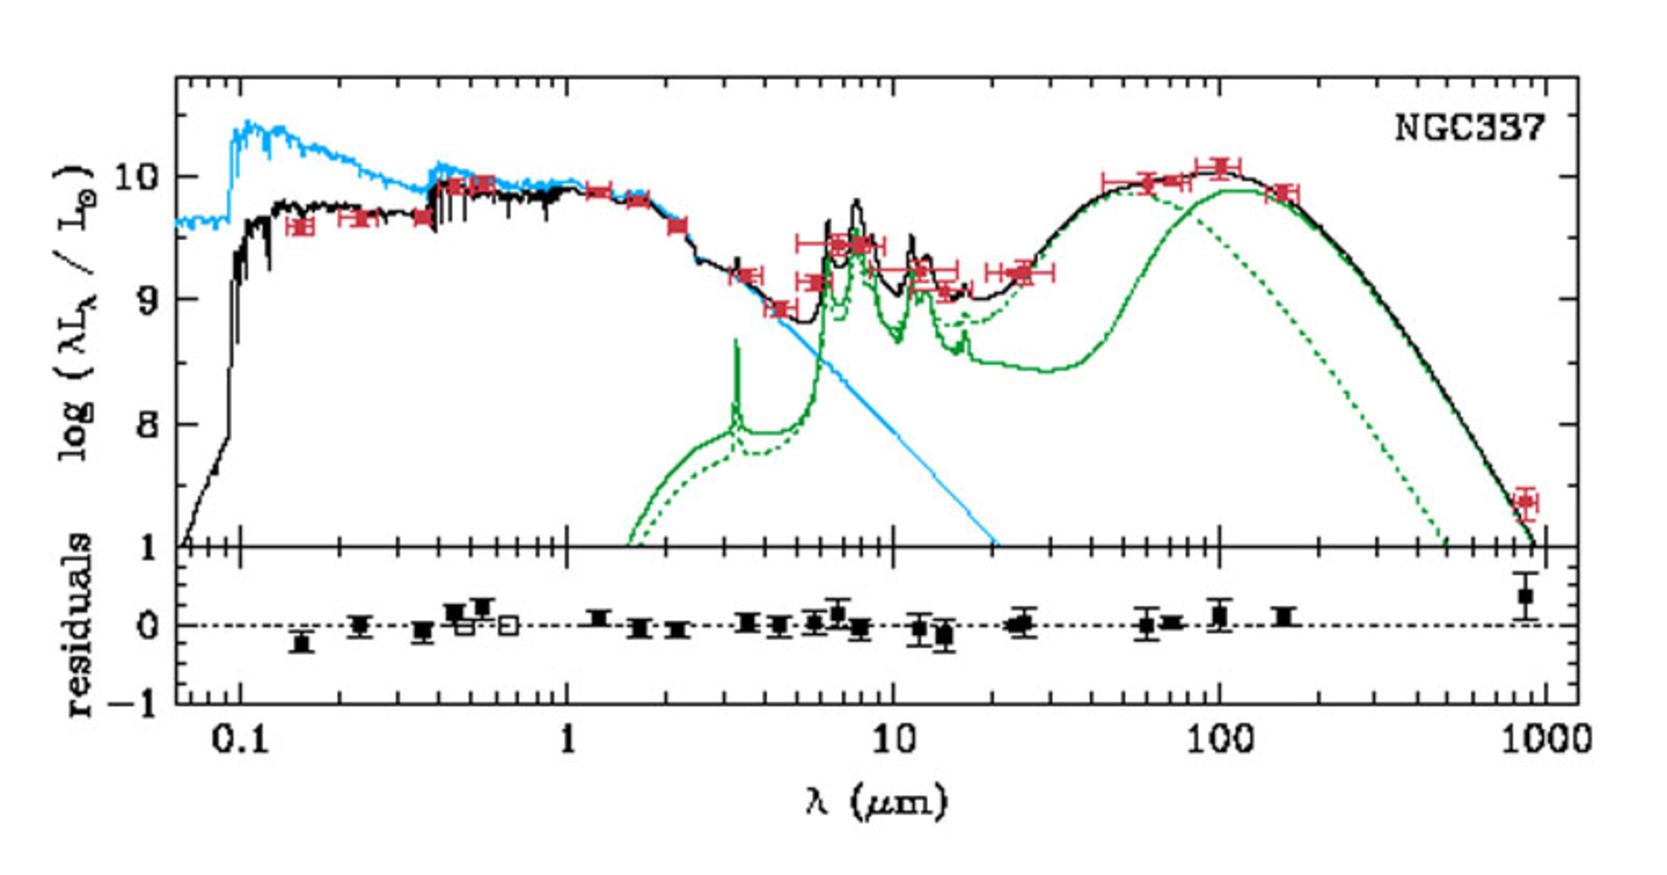
\includegraphics[width=0.9\columnwidth]{Figures/unattenuated_attenuated_sed.pdf}
	\caption[SED of NGC 337]{The best fitting SED model to the observed spectra of NGC 337 adapted from \citealt{daCunha_2008}. The blue line represents the unattenuated stellar spectrum and the green lines show the reprocessed light by dust, separated into dust in the diffuse ISM (solid) and dust in molecular clouds (dotted). The attenuated (observed) SED from the UV to far-IR is shown as the black line, which is fitted to the data points (red).}
	\label{fig:unattenuated_attenuated_sed}
\end{figure}

A fundamental assumption that is made throughout this Thesis is that we can trace the hidden star formation in a galaxy via the dust emission observed in the far-IR and sub-mm wavelengths. Figure \ref{fig:interstellar_medium} shows that the dust and gas are well mixed in the ISM of the Galaxy, suggesting that interstellar dust coexists with the gas and thus dust masses may be a useful measure of the total mass of the ISM. Moreover, because most UV emission comes from recent star formation in a galaxy, the reprocessed IR luminosity is often assumed to be directly proportional to the fraction of the energy from star formation that gets absorbed by dust. As a result, studying the emission from dust is vital in our understanding of the hidden star formation, and the properties of the dust are important in our understanding of the conditions required for star formation to occur.

\subsection{The Lifecycle of Dust}
\label{sec:lifecycle_of_dust}

The lifecycle of dust grains, the mechanisms in which they are produced and destroyed, are important in understanding the metal enrichment and stellar evolution of galaxies. Dust can form in a number of ways including in the stellar winds of evolved stars, from the ejecta of supernovae or from forming in situ in the ISM (\citealt{Draine_2009}). Traditionally, the majority of dust was presumed to be formed in the outer envelopes of latter stage stars, such as red giant branch (RGB) and asymptotic giant branch (AGB) stars. These stars have masses of $1 < M_\textrm{star} [M_\odot] < 8$ and are in a late phase of evolution, having left the (stellar) main sequence and formed heavy elements via stellar nucleosynthesis. The metals solidify into grains in the envelopes of RGB and AGB stars and are carried out in into the ISM by stellar winds (\citealt{Whittet_2002}). For more massive stars with $M_\textrm{star} > 8\,M_\odot$, dust can form in the ejecta of supernovae, condensing from the leftover expanding material. The problem with this pathway, however, is that the dust yields from a single supernova are still a matter of debate, with studies observing dust masses in supernova remnants between roughly $0.05\,M_\odot$ and $1\,M_\odot$ (\citealt{Rho_2008, Dunne_2009, Barlow_2010, Matsuura_2011, Gomez_2012, Matsuura_2015, Chawner_2019}). Much of this debate stems from questions about how the dust formed in supernovae may survive the destructive shock waves that are produced (\citealt{Draine_1979, Jones_1996}). The production rate of dust is a key open question, particularly for studies in the early Universe where a \textit{Dust Budget Crisis} has been proposed (e.g. \citealt{Dwek_2007, Michalowski_2010, Valiante_2011}). This refers to the difficulty in explaining the high dust masses observed in high redshift galaxies from dust produced via the Low-Intermediate Mass Stars (LIMS). Above redshifts $\sim 5$, there is little time for significant amounts of dust to be produced from the post main-sequence evolution of LIMS (\citealt{Morgan_2003, DiCriscienzo_2013}). The final production mechanism we mention here is dust formed in situ via grain growth. This method is most effective in the dense ISM, and so is particularly important in molecular clouds. Grain growth occurs when the conditions allow for the grains to form mantles of ice, which allow metals to subsequently stick to the grains (known as \textit{coagulation}, \citealt{Blain_2004}). We have mentioned one way in which dust can be destoyed in the ISM, supernova shocks, but a second process contributing to dust destruction is \textit{sputtering}. Sputtering occurs as the result of the bombardment of gas atoms in dense environments causing the sublimation of the dust grains (\citealt{Barlow_1978, Jones_2004}). The combination of production and destruction mechanisms form a cyclical nature to dust in the ISM; dust is formed from stellar environments, they are expelled into the ISM and take an enriched form, they get incorporated into molecular clouds, which subsequently leads to star formation and the cycle repeats.

\section{Observing Dusty Star Forming Galaxies in the Far-IR and Sub-mm}

The long wavelengths covering the thermal dust emission can have several names, sometimes referred to as the far-infrared, and at other times as the sub-millimeter. While the two terms are used rather interchangeably, we shall continue with the convention that the far-infrared waveband extends from roughly $10$ to $400\,\mu$m, while the sub-millimeter waveband extends from $400\,\mu$m to $1\,$mm. The peak in the dust emission for most galaxies is located at approximately $100\,\mu$m, where the Cosmic Infrared Background (CIB) peaks (\citealt{Yan_2022}), so in our system the far-IR typically refers to observations that constrain the peak of the spectrum, while sub-mm observations generally constrain the Rayleigh-Jeans side of the SED for galaxies at low redshifts.

The majority of the dust in the ISM, by mass, has temperatures of roughly $15 - 25\,$K (\citealt{daCunha_2008}). It is predominantly the thermal emission from this cold dust that we observe in the far-IR and sub-mm regimes. As can be seen in the example SED of Figure \ref{fig:unattenuated_attenuated_sed}, the dust emission creates a steep sub-mm spectrum, the result of which is a negative \textit{K-correction}. A K-correction is a function of wavelength that is applied to the flux of a redshifted galaxy to convert from the observed frame to the galaxy's rest frame. A strong negative K-correction effectively cancels out the dimming of the flux due to cosmological distances, meaning that a galaxy of a given IR luminosity will have an approximately constant sub-mm flux at redshifts between $z = 1$ and $z\sim8$ (\citealt{Casey_2014b}). This wavelength regime therefore allows us to access galaxies at earlier epochs where the optical/near-IR wavelengths with positive K-corrections have succumbed to substantial redshift dimming. The galaxies that are detected in these wavebands are henceforth referred to as Submillimeter Galaxies (SMGs). As we approach the far-IR, climbing up the Rayleigh-Jeans side of the spectrum, the effect of the negative K-correction becomes less strong and the galaxies detected in the far-IR will typically be lower redshift as a result (\citealt{Casey_2014b, Bethermin_2015b, Zavala_2021}). The benefit here, however, is that at the peak of the dust emission the higher flux density allows us to observe large volumes of local galaxies, even when the sensitivity of the far-IR instrument is sub-optimal. As we shall see, this is used to great effect with far-IR instruments that have surveyed large areas of sky. The galaxies that are detected from their far-IR emission do not necessarily have their own naming convention (though throughout this Thesis, we heavily refer to \textit{Herschel}-detected galaxies in reference to the far-IR detected galaxies with the \textit{Herschel Space Observatory}, which are sometimes also seen referred to as \textit{Herschel}-selected Galaxies, or HSGs, in the literature). We consider these galaxies under the blanket term of Dusty, Star Forming Galaxies (DSFGs), which, in its vagueness, also encompasses SMGs. These galaxies may also be likened to the LIRGs, ULIRGs and HyLIRGs defined earlier, depending on their total IR luminosity.

DSFGs are known to be some of the most massive and extreme examples of star forming galaxies, with star formation rates routinely above $100\,M_\odot$yr$^{-1}$ and stellar masses above $10^{10}\,M_\odot$ (\citealt{Borys_2005, Michalowski_2010, Hainline_2011}). The result of having such high star formation rates, these galaxies are highly dust-enshrouded and are reprocessing as much as $95\%$ or more of the emission from young stars to rest frame far-IR (\citealt{Blain_2002, Casey_2014b}). However, as DSFGs are so massive, they sit at the tip of the galaxy stellar mass function and are thus rare compared to more "conventional" or "normal" star forming galaxies (\citealt{Chapman_2005}). As a result, many of the DSFGs observed to date have been found in wide area, blind surveys from single-dish far-IR and sub-mm facilities such as the Submillimeter Common User Bolometer Array (SCUBA and SCUBA-2; \citealt{Holland_1999, Holland_2013}) on the James Clerk Maxwell Telescope (JCMT) (e.g. \citealt{Smail_1997, Hughes_1998}), the \textit{Herschel Space Observatory} (e.g. \citealt{Eales_2010, Elbaz_2011, Oliver_2012}) and AzTEC on JCMT, ASTE and the LMT (e.g. \citealt{Scott_2008, Aretxaga_2011}).

\subsection{The First Submillimeter Galaxies}
\label{sec:first_submm_galaxies}

The atmospheric transmission of far-IR and sub-mm wavelengths is illustrated in Figure \ref{fig:transmission}. It shows the difficulty in observing electromagnetic radiation in these regimes from the ground, with only select pockets of atmospheric windows allowing for ground-based observations. In the shorter wavelength, far-IR waveband, the transmission is minimal and the possibility of a ground-based far-IR instrument is not feasible. As we have seen, the dust emission at longer wavelengths in the sub-mm is typically many times fainter, but does allow for a limited number of atmospheric windows, including two important windows at $450\,\mu$m ($670\,$GHz) and $\sim 850\,\mu$m ($350\,$GHz). Making use of these brief windows, the aforementioned SCUBA was commissioned on the JCMT with simulatenous operation at $450$ and $850\,\mu$m and was soon used to produce the first sub-mm maps (e.g. \citealt{Smail_1997, Barger_1998, Hughes_1998}). These small maps, totalling several square arcminutes, observed a handful of sub-mm bright galaxies that had luminosities much like those of ULIRGs. While sub-mm astronomy was still in its infancy the sample sizes of SMGs were small. However, these small samples were still enough to have important implications on the cosmic star formation history. At the local density of ULIRGs, very few, if any, such galaxies should have been observed in these fields at $z \gtrsim 1$. The fact that these objects were observed at all implied a strong evolution in the cosmic star formation history and, while ULIRGs play an insignificant role in the star formation rate density locally, these galaxies formed a substantial contribution ($\gtrsim 10\%$) at high redshifts $z \gtrsim 1$ (\citealt{Casey_2014b}). 

\begin{figure}
    \centering
	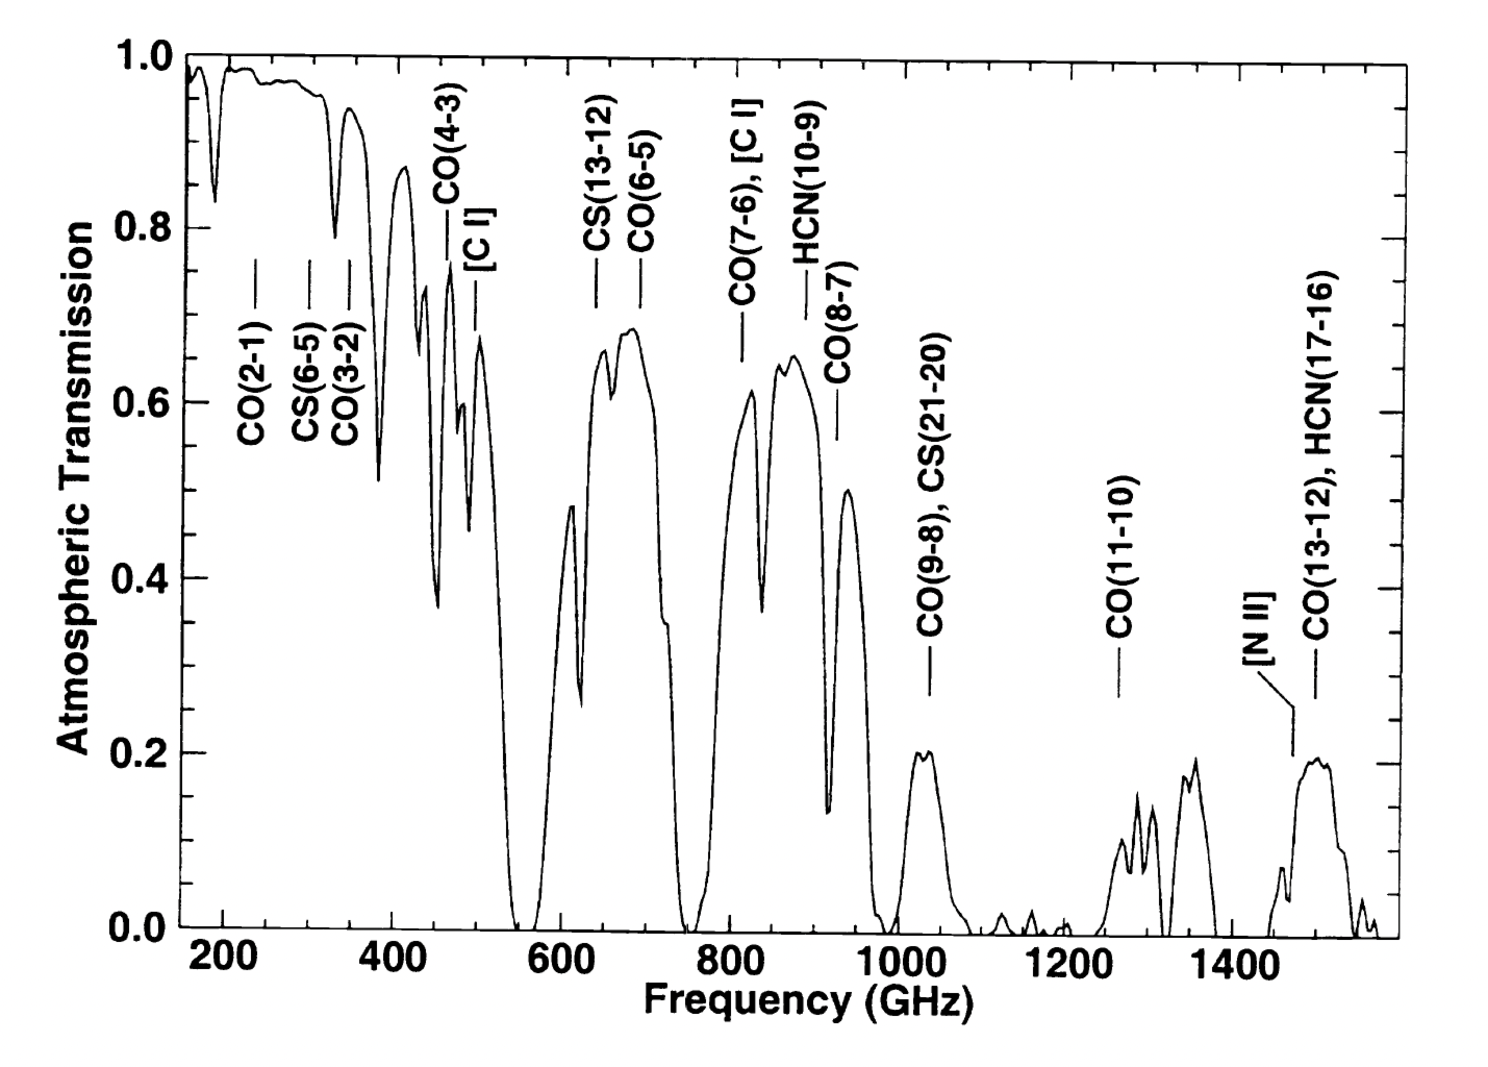
\includegraphics[angle=0.8, origin=c, width=0.8\columnwidth]{Figures/transmission.pdf}
	\caption[Atmospheric transmission of (sub-) mm wavelengths from Pampa la Bola]{The atmospheric transmission spectrum at (sub-)millimeter wavelengths as observed at Pampa la Bola ($4,800\,$m above sea level in Chile) and illustrated in \citealt{Matsushita_2000}. Overplotted are the locations of various CO, CI, CS, NII and HCN transition lines.}
	\label{fig:transmission}
\end{figure}

Let us briefly return to the \textit{Hubble} Deep Field, shown in Figure \ref{fig:hubble_deep_field}. We saw that the field contains a wide variety of galaxies with different morphologies, ages and colours. Importantly we see there are a number of massive ($>10^{10}\,M_\odot$) elliptical galaxies in the local Universe. These galaxies are typically characterized by old stellar populations, limited cold gas and dust, and red colours. The $z = 0$ ages of these galaxies suggest that they had already formed their stellar mass at high redshift (e.g. \citealt{Gallazzi_2005, Thomas_2005}), implying that at some point in the past, they must have been rapidly forming stars and thus be incredibly bright. Without much luck finding these very active galaxies in the optical, the presence of highly dust-enshrouded galaxies with potentially starbursting phases, provides some credit to the idea that SMGs may be the progenitors of these massive elliptical galaxies in the Universe today, namely \textit{proto-ellipticals} (e.g. \citealt{Toft_2014, Valentino_2020b}). A better understanding of this population of galaxies may be key not only in our understanding of the obscured star formation at high redshifts, but also provide a target population in order to study the link between the early and local Universe.

In 1998, SCUBA was used to image the \textit{Hubble} Deep Field at $450$ and $850\,\mu$m; the $850\,\mu$m data covering an area of approximately $9$ square arcminutes. At the time, the map of the \textit{Hubble} Deep Field imaged with SCUBA, presented in \citealt{Hughes_1998}, was the deepest sub-mm map ever taken (a section with radius $100\,$arcsec from the $850\,\mu$m image center is shown in Figure \ref{fig:hubble_deep_field_scuba}). Many of the peaks in the image are a result of source confusion (Section \ref{sec:challenges}), but $5$ reliable sub-mm sources were identified. Despite a comparatively small number of detections compared to the same size area on the \textit{Hubble} image, the total energy outputs are roughly the same. The brightest source, HDF850.1, is an exceptional example of the extreme nature of these sources. HDF850.1 has a star formation rate of $\sim 850\,M_\odot$yr$^{-1}$ (\citealt{Walter_2012}), which is comparable to the total number of stars we expect to be being formed in all the other galaxies in the optical image combined. Moreover, the incredibly dusty nature of this source means that an unambiguous counterpart at shorter wavelengths could not be identified, even in the deepest optical image of the Universe ever taken at the time. The identification of an optical/infrared counterpart has continued to be elusive with only a handful of studies making claims for having identified the galaxy producing the sub-mm emission, with much contention (e.g. \citealt{Dunlop_2004, Serjeant_2014, Sun_2023}).

\begin{figure}
    \centering
	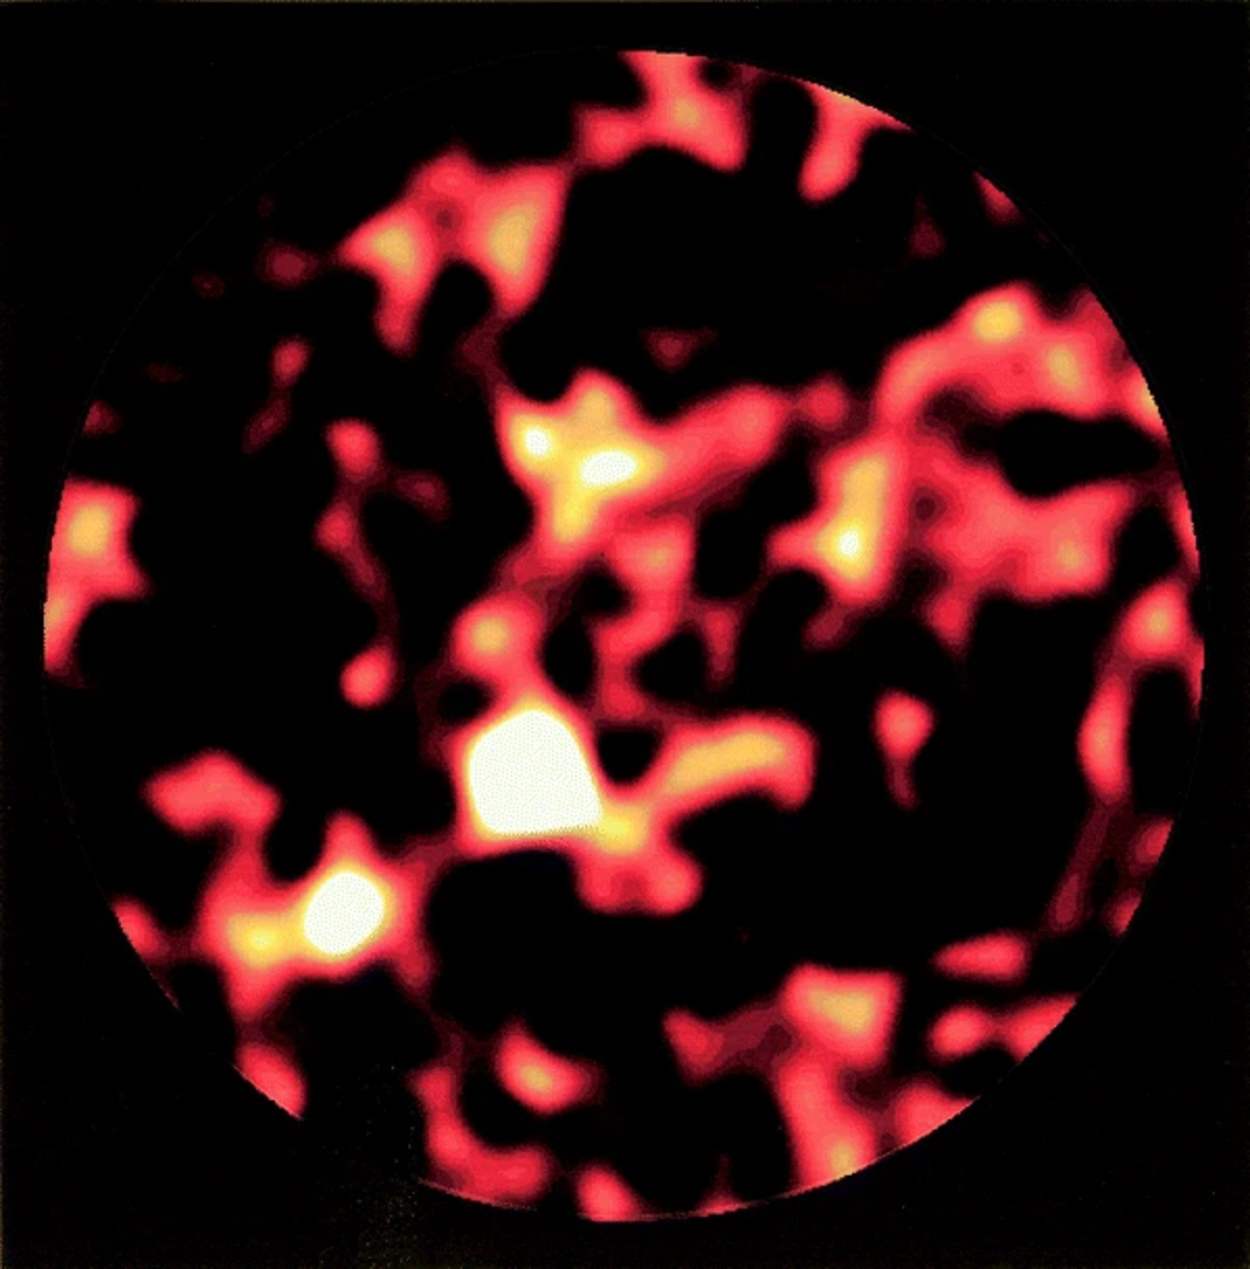
\includegraphics[width=0.8\columnwidth]{Figures/hubble_deep_field_scuba.pdf}
	\caption[Hubble Deep Field as captured by SCUBA on the JCMT]{The $850\,\mu$m map of the \textit{Hubble} Deep Field taken with the SCUBA camera on the JCMT and presented in \citealt{Hughes_1998}. The image is of a patch of the field with a radius of $100\,$arcsec and shows $5$ statistically identified sub-mm galaxies.}
	\label{fig:hubble_deep_field_scuba}
\end{figure}

With continual improvement in the sensitivity of bolometer-arrays, samples of DSFGs detected at sub-mm wavelengths, particularly at $\sim 850\,\mu$m, have continually grown (e.g. \citealt{Borys_2003, Coppin_2006, Weiss_2009, Casey_2013, Geach_2017}). If we wish to observe these same galaxies at far-IR wavelengths closer to the peak of the dust emission we find that the atmospheric transmission falls to zero. These observations are especially vital in characterizing the properties of the dust in these galaxies; without observations constraining the peak of the dust emission basic properties like the mass and temperature of the dust are very hard to predict. The Balloon-borne Large Aperture Submillimeter Telescope (BLAST; \citealt{Devlin_2009}) was an ambitious project to overcome these observational constraints by launching a far-infrared telescope attached to a high-altitude balloon. Above most of the Earth's atmosphere it was able to detect several hundred sources across several flights, but was limited by its large beamsize ($33$, $46$ and $66\,$arcsec at $250$, $350$ and $500\,\mu$m, respectively). Nevertheless, BLAST provided observations that filled in the gap that had been left by other instruments between the long wavelength \textit{Spitzer Space Telescope} bands (up to the $160\,\mu$m band) and the sub-mm wavebands.

\subsection{The \textit{Herschel Space Observatory}}

While BLAST was opening up this key region of the IR spectrum, a new spaceborne telescope was being prepared for launch. Initially called the \textit{Far InfraRed and Sub-millimeter Telescope} (FIRST) but subsequently changed to the \textit{Herschel Space Observatory} (\citealt{Pilbratt_2010}), \textit{Herschel} launched in May 2009 with a $3.5\,$m diameter primary mirror, making it the largest infrared space telescope prior to the launch of the \textit{James Webb Space Telescope} (JWST) on Christmas Day 2021. The mission built upon previous infrared space missions including the \textit{Infrared Astronomical Satellite} (IRAS; \citealt{Neugebauer_1984}), the \textit{Infrared Space Observatory} (ISO), \textit{Spitzer} and AKARI (\citealt{Murakami_2007}), by increasing the collecting area of the mirror and extending coverage to longer wavelengths that had never before been accessible from a space observatory. \textit{Herschel} covered a wide wavelength range from $55$ to $672\,\mu$m, and while its predecessors covered some of this broad part of the spectrum (for example, ISO observed in the wavelength range from $2.5$ to $240\,\mu$m and \textit{Spitzer} obtained imagery and spectra in the range $3$ to $180\,\mu$m), the improved resolution and sensitivity of \textit{Herschel} allowed for more detailed study of the cold dust in galaxies.

The operational wavelength range drives the science objectives of an instrument, in the case of \textit{Herschel}, this range corresponds to the peak continuum emission from bodies with temperatures between $\sim5$ and $50\,$K and the bright molecular and atomic emission lines from gases with temperatures between $10$ and several hundered K (\citealt{Pilbratt_2008}). The thermal radiation from dust grains dominate the emission observed in the \textit{Herschel} range, allowing us to observe star forming molecular clouds at the stellar level within the Galaxy and the integrated properties of actively star forming galaxies at high redshifts. The key science objectives of \textit{Herschel} were based on these capabilities, focusing on the formation and evolution of stars and galaxies and the interaction with the ISM. In particular, the main science drivers were: to survey the extragalactic and Galactic sky in order to measure the obscured star formation activity over cosmic time (Section \ref{sec:cosmic_star_formation_history}); to study the physics and chemistry of the ISM; and to understand the stellar and interstellar lifecycle from observational astrochemistry.

\textit{Herschel} had three instruments onboard: the \textit{Spectral and Photometric Imaging Receiver} (SPIRE; \citealt{Griffin_2010}); the \textit{Photodetector Array Camera and Spectrometer} (PACS; \citealt{Poglitsch_2010}); and the \textit{Herschel-Heterodyne Instrument for the Far-Infrared} (HIFI; \citealt{deGraauw_2010}). In the context of this Thesis, we shall be mainly focused on the photometric capabilities of PACS and SPIRE. PACS was operational as both an imaging photometer and an integral field spectrometer. The imaging photometer had three broadband photometric bands centered at $70\,\mu$m ($60 - 85\,\mu$m), $100\,\mu$m ($85 - 130\,\mu$m) and $160\,\mu$m ($130 - 210\,\mu$m), which could observe simultaneously at $160\,\mu$m and one of the $70$ or $100\,\mu$m bands. These wavebands were ideally placed to study the peak of dust emission in local galaxies. The beamsizes of the PACS instrument depended on the scan rate being used, but were typically of order $5$, $7$ and $12\,$arcsec at $70$, $100$ and $160\,\mu$m, respectively (\citealt{Poglitsch_2010}). SPIRE, also a spectrometer and an imaging photometer, operated simultaneously in three wavebands centered at $250$, $350$ and $500\,\mu$m. Due to the longer wavelengths than PACS, the SPIRE beamsizes were larger at $18$, $26$ and $36\,$arcsec for $250$, $350$ and $500\,\mu$m, respectively, with larger confusion limits of approximately $5.8$, $6.3$ and $6.8\,$mJy (\citealt{Griffin_2010}). While the beamsizes are large, we note the marked improvement over the BLAST values quoted earlier. Combined with the fast mapping speed, the large beamsize allowed SPIRE to image areas of sky quickly, making it useful for covering wide extragalactic surveys (\citealt{Eales_2010, Oliver_2012, Holder_2013, Viero_2014}). Finally, HIFI, which does not feature in this Thesis, was a high resolution heterodyne spectrometer. Observing just a single pixel on the sky at a time, HIFI produced extremely detailed spectra of the molecules in a galaxy.

\subsection{\textit{Herschel} Surveys}

The launch of \textit{Herschel}, particularly with the mapping speed of the SPIRE instrument, allowed, for the first time, large scale surveys at wavelengths between $\sim 100$ and $500\,\mu$m. The rapid technological advancement in far-IR/sub-mm astronomy becomes clear when one compares the maps produced during \textit{Herschel}'s legacy programes with the first sub-mm images (e.g. Figure \ref{fig:hubble_deep_field_scuba}). As an example, Figure \ref{fig:gama9} shows one field, GAMA9, from the \textit{Herschel}-ATLAS project (which we shall describe in more detail in Chapter \ref{chapter:Data_Release_3}), spanning approximately $54\,$deg$^2$. A preliminary data release, named the Science Demonstration Phase (SDP; \citealt{Ibar_2010, Rigby_2011, Pascale_2011}), focused on PACS and SPIRE photometry of one panel of the GAMA9 field (the second rectangular region from the left in Figure \ref{fig:gama9}), totalling $16\,$deg$^2$. This field contained almost $10,000$ galaxies and took \textit{Herschel} just $16$ hours to image. We compare this to the SCUBA Hubble Deep Field map, which took a total of $51$ hours to image an area approximately $600$ times smaller, detecting only $5$ secure sub-mm sources. This highlights the vast improvement in mapping speed and observing time required per source that had been made in the decade leading up to the launch of \textit{Herschel}.

\begin{figure}
    \centering
	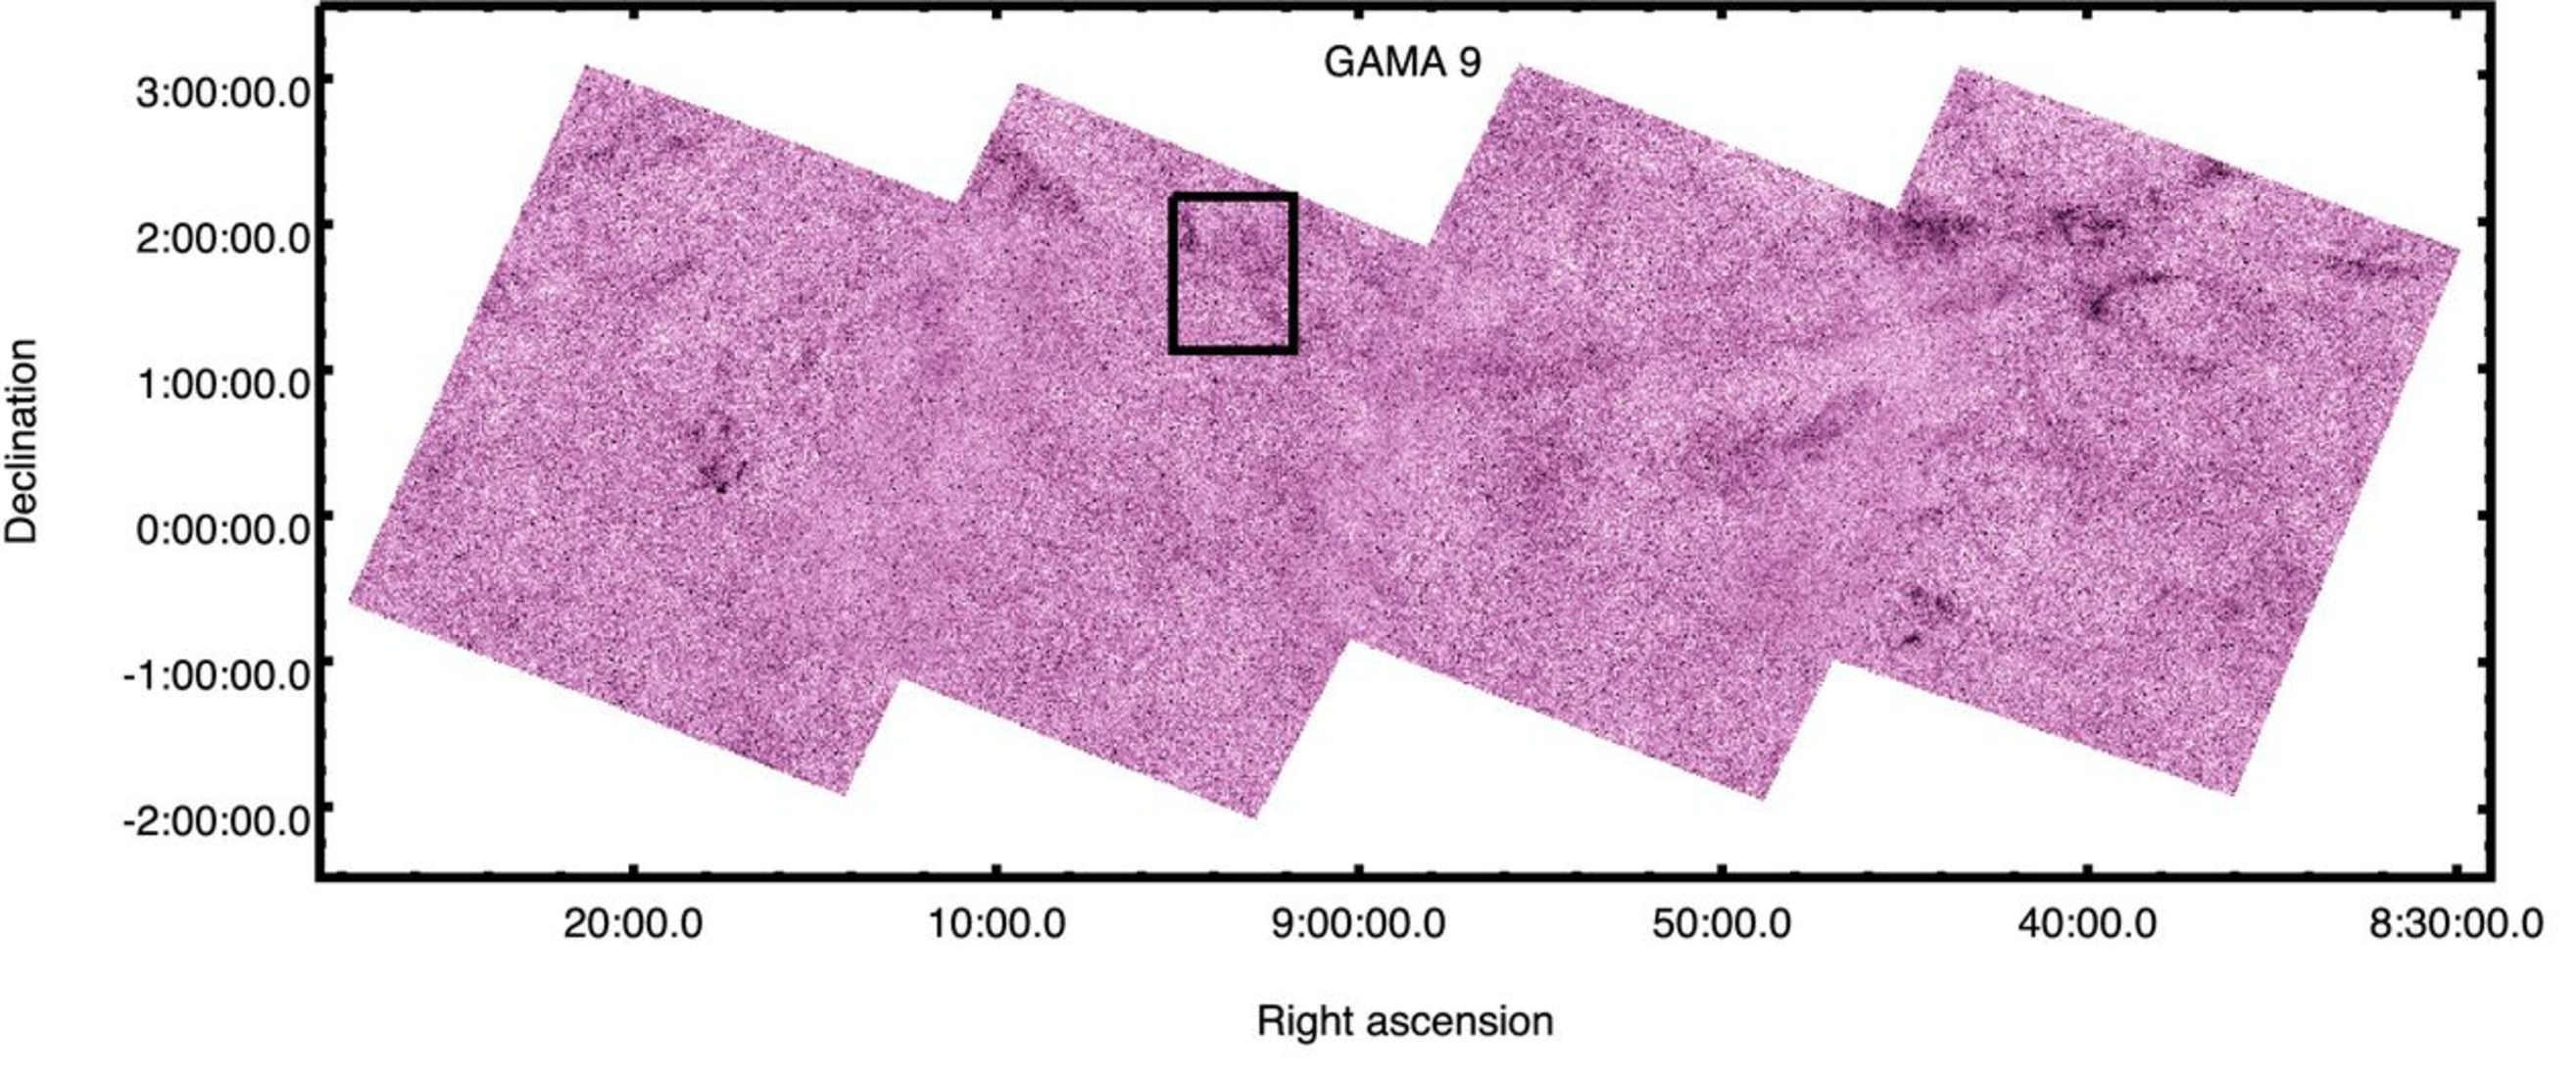
\includegraphics[width=0.9\columnwidth]{Figures/GAMA9.pdf}
	\caption[$250\,\mu$m map of the GAMA9 field of H-ATLAS]{The $250\,\mu$m image of the GAMA9 field of the \textit{Herschel}-ATLAS. The Science Demonstration Phase (SDP) of the H-ATLAS project observed the second rectangular region from the left, which has an area of approximately $16\,$deg$^2$. The total area of the GAMA9 field is approximately $54\,$deg$^2$. The figure is as presented in \citealt{Valiante_2016}. {\color{red}Figure without rectangle drawn?}}
	\label{fig:gama9}
\end{figure}

In total, extragalactic surveys with \textit{Herschel} exceed $1,000\,$deg$^2$ in area. During this Thesis we will be mainly focused on two \textit{Herschel} surveys, the \textit{Herschel}-Astrophysical Terahertz Large Area Survey (H-ATLAS; \citealt{Eales_2010}) and the \textit{Herschel} Multi-tiered Extragalactic Survey (HerMES; \citealt{Oliver_2012}). Both surveys will be described in detail, H-ATLAS in Chapter \ref{chapter:Data_Release_3} and HerMES in Chapter \ref{chapter:Radio_Identifications}. Figure \ref{fig:herschel_surveys} shows the area of various \textit{Herschel} surveys against the point source depth, showing that HerMES consists of a range of shallow and wide fields and deep and narrow fields, and that the \textit{Herschel}-ATLAS was the largest extragalactic survey in open time, spanning approximately $660\,$deg$^2$ in total. H-ATLAS was designed to be a shallow survey that could rapidly map a large area of sky, detecting hundreds of thousands of galaxies from their cold dust emission. This survey forms the cornerstone of this Thesis, allowing us to measure the evolution of the dusty ISM for a large number of galaxies in the past several billion years of cosmic history.

\begin{figure}
    \centering
	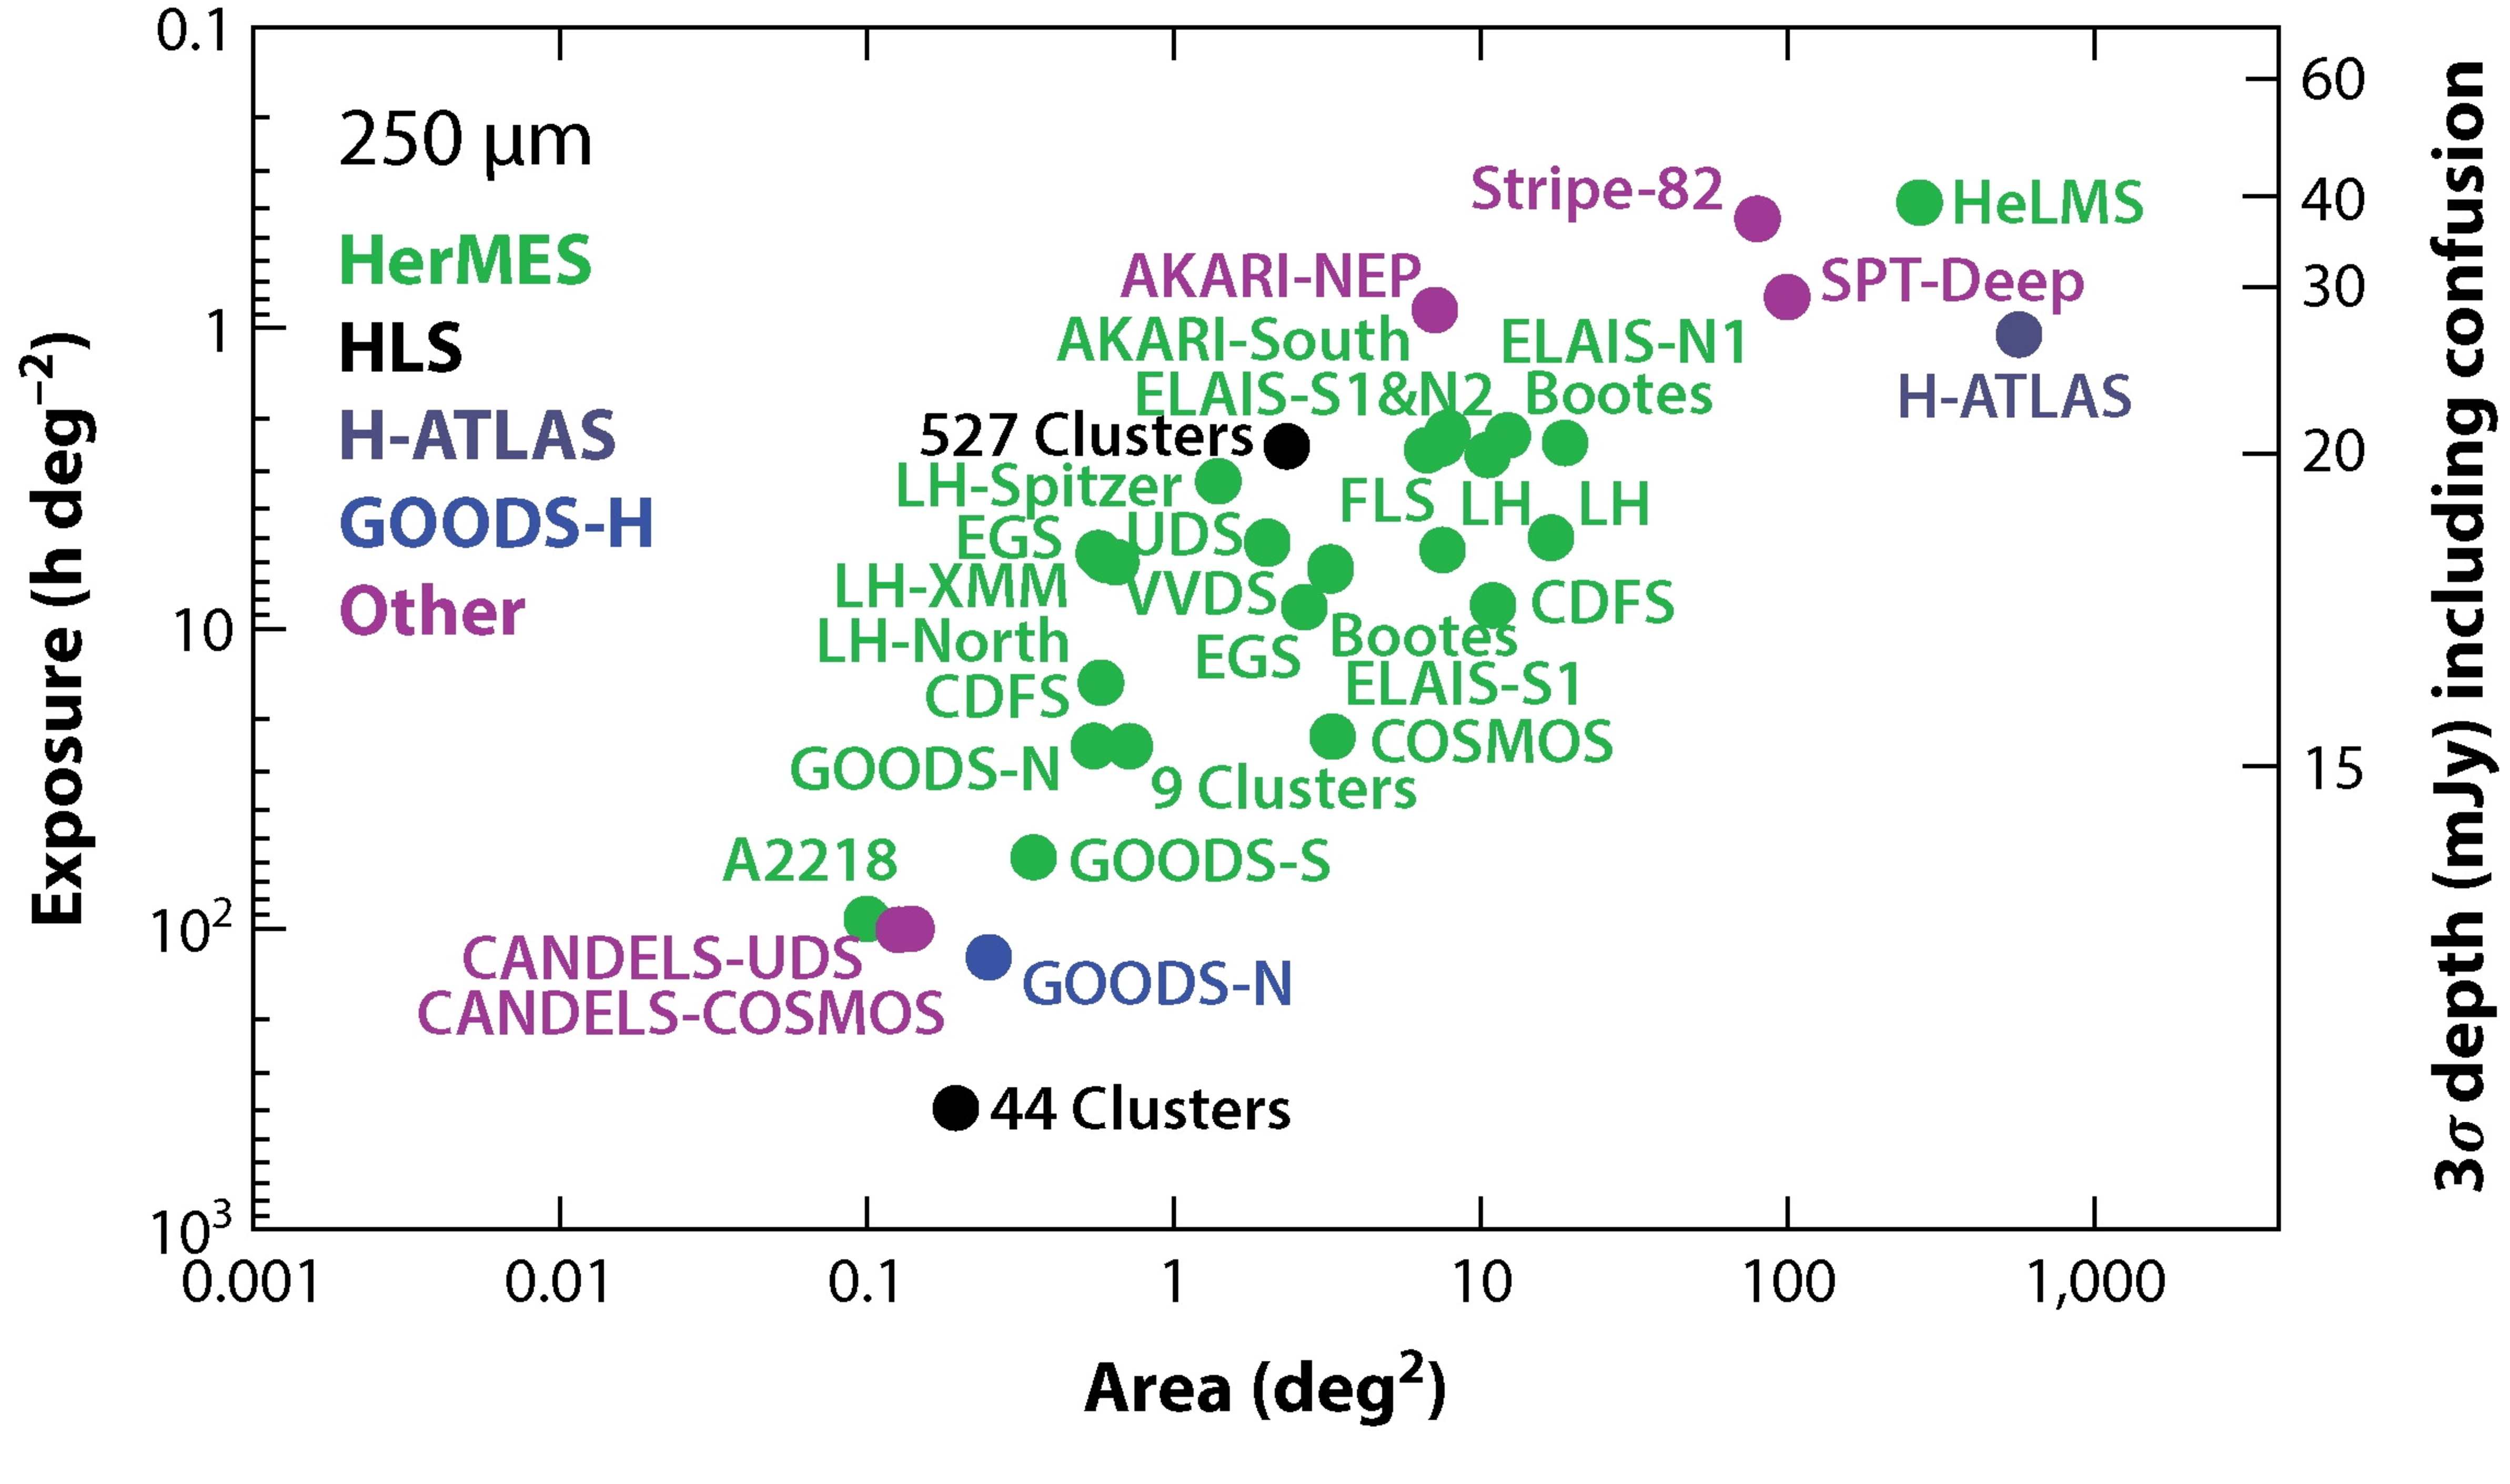
\includegraphics[width=0.9\columnwidth]{Figures/herschel_surveys.pdf}
	\caption[Survey area against point source depth for extragalactic \textit{Herschel} surveys]{The survey area against the point source depth of a selection of extragalactic surveys at $250\,\mu$m with \textit{Herschel}, as presented in \citealt{Lutz_2014}. The figure shows the fields that form the following surveys: the \textit{Herschel} Multi-tiered Extragalactic Survey (HerMES, green circles); \textit{Herschel} Lensing Survey (HLS, black circles); \textit{Herschel}-Astrophysical Terahertz Large Area Survey (H-ATLAS, dark blue circles) and Great Observatories Origins Deep Survey - Herschel (GOODS-H, blue circles).}
	\label{fig:herschel_surveys}
\end{figure}

\section{Challenges in Identifying DSFGs and their Multiwavelength Counterparts}
\label{sec:challenges}

The reason why the far-IR and sub-mm regions of the electromagnetic spectrum have been elusive to astronomers until very recently is partly due to the difficulties in constructing the instruments and telescopes required for these wavelengths. As we saw in Section \ref{sec:first_submm_galaxies}, one obstacle is the atmospheric absorption caused by water vapour in the Earth's atmosphere, requiring far-IR and sub-mm telescopes to be located at high-altitude sites or in space. Adding to this, the cameras themselves are not like the typical photodetectors that may be used at other wavelengths, but instead are \textit{bolometers} that detect infrared radiation by measuring the increase in temperature when radiation gets absorbed (\citealt{Woodcraft_2009}). The first bolometer was built by Samuel Pierpont Langley in 1880 (\citealt{Langley_1880}), and were initially limited to single-pixel devices. The breakthrough for sub-mm astronomy came with the first bolometer cameras in the 1990s, which linked multiple bolometers together to make a multi-pixel camera. However, the difficulty in applying these newly discovered bolometer cameras to observing thermal radiation from dust is that the thermal radiation from the instruments themselves will cause substantial noise. This requires operating them at ultra-low temperatures. \textit{Herschel} carried coolant to cryogenically cool the detectors to $\sim 300\,$mK and the rest of the observatory to $1.7\,$K, but this meant that the lifespan of the telescope was predetermined to the conservation time of the liquid helium reserve (\textit{Herschel} was operational for four years between 2009 and 2013). Moreover, for a spaceborne observatory, the size of the primary mirror is restricted by the limitations of launching the telescope to space (although some novel approaches like the folding mirrors of JWST have increased the light collecting area we have in space). This is problematic given that the resolution of a telescope is dependent on the diameter of the primary mirror, $D$, and the observing wavelength, $\lambda$, according to $\theta = 1.22\lambda/D$. The long wavelength sub-mm bands and the restrictions on mirror size, particularly for spaceborne telescopes, means that the angular resolutions of sub-mm telescopes are typically poor.

The result of low angular resolution is source confusion. This occurs when more than one source is present in the observing beam due to the faint signals from unresolved sources (\citealt{Condon_1974}). As fainter objects far outnumber brighter objects, far-IR/sub-mm surveys have a minimum flux density below which you become confusion limited and the number of DSFGs that can be observed is highly dependent on them being high significance detections in order to avoid counting spurious peaks in the noisy maps. This limitation is emphasized by an effect that was earlier presented as an advantage of the far-IR/sub-mm bands: the negative K-correction. These wavebands are particularly susceptible to source confusion because the negative K-correction causes distant galaxies to appear in images with comparable brightness to nearer galaxies, meaning a greater chance of multiple faint objects being present within a single beam.

The optical to IR counterparts of our DSFGs are used to derive photometric redshifts as well as basic properties such as their stellar mass and star formation rates. This multiwavelength view of a galaxy is important in obtaining a full picture of the galaxy population and their evolution, however, characterizing our galaxies at other wavelengths could lead to a biased view of the population if we cannot localize the counterparts for a complete sample of DSFGs. The large beamsize of single-dish sub-mm observations means that these sources typically have positional uncertainties of several arcseconds and there can be many possible counterparts close to the location of the dust emission. Figure \ref{fig:viking_cutout} shows a region $12\times12\,$arcsec around a \textit{Herschel} source detected in H-ATLAS (black cross). The figure shows the VISTA Kilo-degree Infrared Galaxy (VIKING) survey $K_s$ band image of the same region, showing two potential near-IR counterparts highlighted red and blue (\citealt{Fleuren_2012}). Such a scenario where it is not trivial to locate the true source of the dust emission is not uncommon (e.g. \citealt{Ivison_2002, Pope_2006, Chapin_2011, Smith_2011, Kim_2012, Alberts_2013, Bourne_2016, Furlanetto_2018}). The most reliable way of refining the position of the source is to use interferometric observations with the likes of the Atacama Large Millimeter/submillimeter Array (ALMA) to secure the position to approximately arcsec resolution (e.g. \citealt{Karim_2013, Hodge_2013, Miettinen_2015,Simpson_2015, Fujimoto_2016}), however, this is impractical for large surveys, and to crossmatch all our far-IR/sub-mm sources with their multiwavelength counterparts, without the use of expensive, targeted observations, we must find alternative methods that directly match to our low resolution observations.

\begin{figure}
    \centering
	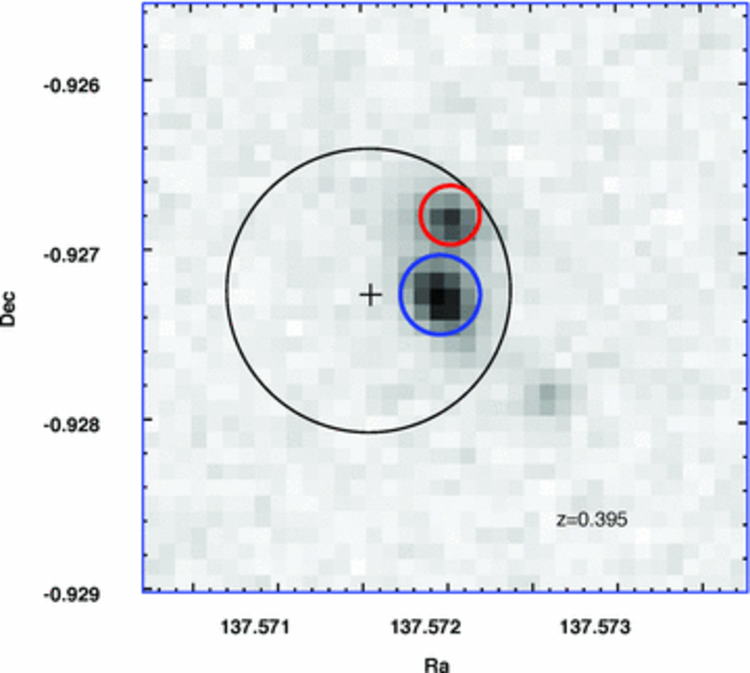
\includegraphics[width=0.8\columnwidth]{Figures/viking_cutout.pdf}
	\caption[VISTA-VIKING cut-out of H-ATLAS J091017.1-005538]{A VISTA-VIKING cut-out of H-ATLAS J091017.1-005538 in the $K_s$ band ($2.15\,\mu$m) from \citealt{Fleuren_2012}. The location of the far-IR emitting region is indicated by a black cross with a $2\sigma = 2.9\,$arcsec positional uncertainty for this source represented by a black circle. Two potential near-IR counterparts are highlighted by red and blue circles; a third with negligible probability of being the true association can be seen outside the $2.9\,$arcsec radius. {\color{red}Potentially replace this with a better figure?}}
	\label{fig:viking_cutout}
\end{figure}

\section{Outline of Thesis}

In this Thesis we study several open questions about interstellar dust in active star forming galaxies. We study a sample of \textit{Herschel} detected galaxies at $z < 1$ and derive the evolution of their dust content, spanning the past $8$ billion years, closing in on the peak in cosmic star formation. At higher redshifts, we study the dust properties of a sample of DSFGs to test whether the common assumption of extragalactic studies, that the properties of dust are the same at all epochs, holds true by comparison with local values. Finally, we identify a sample of \textit{Herschel} galaxies for which we have robust UV-IR spectra to understand the role that they play in the dust obscured star formation activity of the Universe and their stellar mass assembly histories. The following is an outline of each Chapter:

\begin{itemize}
	\item In Chapter \ref{chapter:Data_Release_3}, we introduce the \textit{Herschel}-ATLAS survey and conduct a thorough Bayesian analysis, namely the Likelihood Ratio method, to identify near-IR counterparts to \textit{Herschel} sources in the South Galactic Pole (SGP) field. We also present a new method in which to predict the number of potential strong and weak gravitational lensing events within a blank \textit{Herschel} field, with no constraints from a minimum \textit{Herschel} flux density. The majority of the research from this chapter can be found in \citealt{Ward_2022}.
	\item In Chapter \ref{chapter:Dust_Mass_Functions}, we use the SGP sample from the previous chapter to measure the dust mass function (DMF) from $\sim80,000$ galaxies out to $z = 1$. We use our DMFs to derive the cosmic dust mass density over the past $8\,$Gyr and compare the evolution in the dust content of the Universe with the star formation rate density. The work estimating the dust temperatures of H-ATLAS galaxies is used in \citealt{Eales_2024}.
	\item In Chapter \ref{chapter:Dust_Evolution}, we present two samples of DSFGs that span redshifts between $z = 2$ and $z = 6$, one \textit{Herschel} selected as part of the \textit{Herschel Bright Sources} (HerBS) sample, and the other sample selected at $1.4\,$mm as part of the South Pole Telescope -- Sunyarv-Zel'dovich survey. Together, a total of approximately $100$ galaxies are used to predict the average dust properties of high redshift star forming galaxies, which we compare with local samples to test whether dust takes the same form at all times of cosmic history. The research from this chapter is presented in \citealt{Ward_2024}.
	\item In Chapter \ref{chapter:Radio_Identifications}, we turn to the \textit{Cosmic Evolution Survey} (COSMOS) where approximately $10,000$ \textit{Herschel} galaxies have been observed as part of HerMES, along with $\sim10,000$ VLA sources at $3\,$GHz. We make use of the well-studied relationship between the far-IR and radio emission of star forming galaxies to identify highly probable radio counterparts which, with their good astrometric precision, allows for the unambiguous matching with multiwavelength associations. With exceptional coverage across the UV to far-IR spectrum for a large sample of \textit{Herschel} galaxies, we investigate their evolutionary state and the stellar mass assembly history of such galaxies.
	\item In Chapter \ref{chapter:Conclusion}, we provide a summary of our key findings from the Thesis and present potential avenues for future studies related to the research presented herein.
\end{itemize}

Through this work we attempt to answer the following questions; which we shall return to in our closing discussion. How has the dust content of galaxies evolved to the present day? Are the dust properties of galaxies the same at all cosmic epochs? And in what evolutionary stage do we observe dust-enshrouded, IR-bright galaxies; do they provide the link to the massive systems we observe in the local Universe today?



\chapter{Herschel-ATLAS Data Release III}
\label{chapter:Data_Release_3}
\sloppy

\section{Introduction}

We have already seen that the poor angular resolution of long wavelength instruments such as SPIRE (the FWHM of $250\,\mu$m detections is $\sim18\,$arcsec, as predicted by the equation $\theta = 1.22\lambda/D$), cause large positional uncertainties, and force us to increase the search radius around each source to look for counterparts. This effect, coupled with the intrinsic faintness of optical associations due to dust obscuration, the relatively flat redshift distribution of far-IR sources due to the k-correction, and the high surface density of objects in optical surveys, means that multiple possible counterparts are often observed within a given radius. For small far-IR/sub-mm surveys, it was most practical to first match with radio or mid-IR sources and then use pre-existing catalogues to obtain multiwavelength data. However, presently this is not suitable for large \textit{Herschel} surveys as current mid-IR and radio surveys, or interferometric follow up surveys, do not cover sufficiently large areas to match with more than a small fraction of the sources detected on the far-IR/sub-mm images (e.g. \citealt{Chapman_2005, Ivison_2007, Dye_2008, Dye_2009, Biggs_2011, Simpson_2015}). While upcoming surveys from radio facilities such as the Square Kilometer Array (SKA), the Low Frequency Array (LOFAR) and MeerKAT will increase the radio coverage of the \textit{Herschel} fields, currently, the most appropriate way to decide which objects are associated to such large samples of \textit{Herschel} sources is to use a statistical identification technique using optical and/or infrared surveys.

In the following, we present the \textit{Herschel}-ATLAS project and the data products that have been released, which include the maps and catalogues of \textit{Herschel} sources and their most probable optical/near-IR counterparts. These were identified using a Bayesian approach that assigns probabilities to each possible counterpart and selects the single galaxy with the highest probability. We present an application of this method to the sources in the South Galactic Pole field, covering $\sim50\%$ of the survey area, which have yet to be statistically matched to galaxies observed at optical/IR wavelengths.

\section{The Herschel-ATLAS}
\label{sec:The Herschel-ATLAS}

The \textit{Herschel} Astrophysical Terahertz Large Area Survey (H-ATLAS; \citealt{Eales_2010}) was the largest open-time far-IR survey carried out with the \textit{Herschel Space Observatory}. The survey area was observed in five photometric bands using the two photometers mentioned previously: PACS at $100$ and $160\,\mu$m, and SPIRE at $250$, $350$ and $500\,\mu$m. Compared to the first SMGs detected using SCUBA at $850\,\mu$m, the PACS and SPIRE wavebands span the peak of the thermal dust emission for low redshift ($z < 1$) galaxies and thus their intrinsic brightness at the SPIRE wavelengths makes their detection in the thousands possible over large areas. The main scientific goal of the survey was to estimate the dust masses and dust obscured star formation rates for thousands of nearby galaxies over a large fraction of sky, however, the sensitivity of \textit{Herschel}, aided by the negative K-correction at the SPIRE wavelengths (\citealt{Blain_1993}), meant that a substantial fraction of sources were observed at higher redshifts, with a median of $z \sim 1$. The catalogues of the survey, as detailed below, includes sources with redshifts up to $\sim 6$ (\citealt{Amblard_2010, Lapi_2011, Fudamoto_2017, Zavala_2018}).

The complete survey covers $\sim 660\,$deg$^2$, split into three regions that are located to avoid emission from Galactic dust and to make the most of complementary spectroscopic surveys including the Sloan Digital Sky Survey (SDSS, \citealt{York_2000}), the 2df Galaxy Redshift Survey (2dfGRS, \citealt{Colless_2001}) and the Galaxy and Mass Assembly (GAMA, \citealt{Driver_2009}). The three regions are: The North Galactic Pole (NGP) field covering $\sim 180\,$deg$^2$ of the northern sky, centered at R.A 13$^{h}$18$^{m}$ and declination +29$^{\circ}$13' (J2000); three equatorial fields, located at approximately R.A 9$^{h}$, 12$^{h}$ and 15$^{h}$ coinciding with the GAMA survey (also known as GAMA9, GAMA12 and GAMA15), each with an area of approximately $54\,$deg$^2$; and the South Galactic Pole (SGP) field, centered at R.A 0$^{h}$6$^{m}$ and declination -32$^{\circ}$44' (J2000) with an area of $\sim 318\,$deg$^2$. 

\subsection{Detecting Far-IR Sources on \textit{Herschel} Images}
\label{sec:Detecting Submillimeter Sources on Herschel Images}

Partly due to the poor angular resolution of \textit{Herschel}, the far-IR images contain two main types of noise: instrumental noise (such as the noise from the thermal emission of the telescope), which is not typically correlated between pixels, and confusion noise which is highly correlated between pixels - most of its contribution coming from the blending together of faint sources. The result of combining instrumental noise with confusion noise is that almost all sources in the \textit{Herschel} images are unresolved and the optimum filter for recovering these sources is no longer a simple point spread function (PSF). Let us briefly consider two \textit{Herschel} images in which there is only one source of noise at a time. First, an image with instrumental noise but no confusion noise (i.e. there is only one point source and no fainter, confusing objects). For this image, the optimal detection of this source is obtained by convolving the image with the PSF of the instrument. If we instead consider all confusion noise (i.e. there is no instrumental noise, but many confused sources), the far-IR source would be recovered from the image with optimal signal to noise by taking the Fourier transform of the image, dividing by the Fourier transform of the PSF and taking the inverse Fourier transform of the result to obtain a perfect deconvolution of the original map (\citealt{Valiante_2016}). However, for a variable combination of the two, \citealt{Chapin_2011} showed that a convolving function or \textit{matched filter} can be calculated to provide the maximum signal to noise ratio (SNR) for unresolved sources.

To detect sources from the $250\,\mu$m maps using the matched filter (the $250\,\mu$m band is the most sensitive of the SPIRE bands and given the lower sensitivity of the PACS instrument, all sources detected on the PACS images would also be detected on the SPIRE $250\,\mu$m image), \citealt{Maddox_2020} developed a source detection algorithm called the Multi-band Algorithm for Source Detection and eXtraction (\texttt{MADX}). \texttt{MADX} works by first removing Galactic dust emission from the image using \texttt{Nebuliser}, then convolving the image with the matched filter. The variance maps, from which the flux density errors of the sources are determined, were created by convolving the map of instrumental noise with the matched filter and adding on the typical confusion noise level. The same process was applied to the $350$ and $500\,\mu$m images, however, due to the smaller PSF at $250\,\mu$m, and thus more accurate source positions, zero weighting was given to the $350$ and $500\,\mu$m images when generating the detection map from which sources were located. In effect, the detection map was the same as the $250\,\mu$m map.

Sources were identified by peak values $> 2.5\sigma$ in the filtered detection map and their positions were estimated by fitting a Gaussian to the nearest pixels surrounding the location of the peak. The source was extracted in the other \textit{Herschel} wavebands at the location of $250\,\mu$m position. The final catalogues contained those sources with SNR $> 4$ in any of the three SPIRE bands. The zero weighting of the $350$ and $500\,\mu$m images might suggest that we miss sources that are faint at $250\,\mu$m but bright at $350$ and $500\,\mu$m, but by cataloguing all sources with SNR $> 4$ in any of the SPIRE bands means that the catalogues are reasonably complete in all bands. The completeness of the \textit{Herschel} catalogues are shown in Figure \ref{fig:submm_completeness} as a function of the measured flux density at each SPIRE band.

\begin{figure}
    \centering
	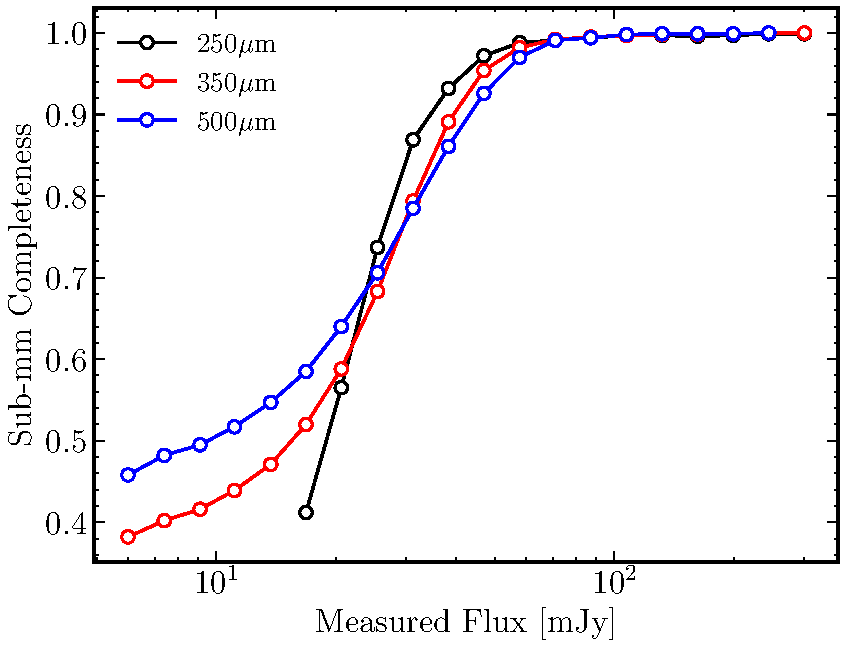
\includegraphics[width=0.8\columnwidth]{Figures/submm_completeness.pdf}
	\caption[Completeness of H-ATLAS DR1 catalogue as a function of $250\,\mu$m flux]{The completeness of the Data Release I catalogues of \textit{Herschel} sources, as a function of the measured flux density at $250\,\mu$m (black) $350\,\mu$m (red) and $500\,\mu$m (blue). This figure is recreated from Figure 21 in \citealt{Valiante_2016}.}
	\label{fig:submm_completeness}
\end{figure}

\subsection{Data Releases of the H-ATLAS}
\label{sec:Data Releases of the H-ATLAS}

The first public data release (DR1) of H-ATLAS covered the three equatorial GAMA fields, which cover approximately $25\%$ of the total survey area. These fields benefit from multiwavelength coverage from GAMA, SDSS, 2dF, the Galaxy Evolution Explorer (GALEX, \citealt{Martin_2005}), the UKIRT Infrared Deep Sky Survey -- Large Area Survey (UKIDSS-LAS, \citealt{Lawrence_2007}), the Wide-field Infrared Survery Explorer (WISE, \citealt{Wright_2010}), the VISTA Kilo-degree Infrared Galaxy survey (VIKING, \citealt{Edge_2013}) and the Kilo-Degree Survey (KiDS, \citealt{deJong_2013}). Combined across the three fields, there are a total of $113,995$, $46,209$ and $11,011$ sources detected at $> 4\sigma$ at $250$, $350$ and $500\,\mu$m, and $4,650$ and $5,685$ sources detected at $> 3\sigma$ at $100$ and $160\,\mu$m, respectively (\citealt{Valiante_2016}). Following the release of the DR1 sources, \citealt{Bourne_2016} used the Likelihood Ratio method (LR; \citealt{Sutherland_1992, Ciliegi_2003}) to identify probable optical SDSS counterparts to the sources with SNR$_{250} > 4$. We shall discuss the method in detail in Section \ref{sec:The Likelihood Ratio Method}. Sources with SNR$_{250} < 4$ that were in the DR1 catalogue due to significant $350$ or $500\,\mu$m detections were omitted from the analysis of \citealt{Bourne_2016} on the basis that they have far-IR colours indicating high redshifts, and are more likely to be misidentifed due to the increased probability of chance aligments or the effects of gravitational lensing along the line of sight \mbox{(\citealt{Negrello_2010, Pearson_2013, Bourne_2014}).}

The second public data release (DR2) covered the NGP and SGP, that together form $\sim 75\%$ of the total survey area. The NGP has coverage at optical wavelengths from the SDSS, and in the near-IR by UKIDSS-LAS. Moreover, a smaller $\sim26\,$deg$^2$ area of the field was observed by a deeper $K_s$-band survey by the H-ATLAS team using the UKIRT (with a limiting magnitude in the Vega system of $K_s = 19.40$, compared to $18.69$ for UKIDSS-LAS). The SGP is the largest field, spanning approximately half of the total H-ATLAS survey area, and has coverage from the 2dF spectroscopic survey, KiDS in four optical bands ($u$, $g$, $r$ and $i$) and VIKING in five near-infrared bands ($Z$, $Y$, $J$, $H$ and $K_s$). The DR2 \textit{Herschel} source catalogues are obtained from areas of the images that have at least two observations from the SPIRE instrument, the second pass significantly reducing the total noise at the positions of all sources, meaning that the areas covered by the catalogues are slightly smaller than the images ($177\,$deg$^2$ for the NGP and $303\,$deg$^2$ for the SGP).

The DR2 catalogues, obtained in the same manner as the first data release, contain $118,980$ sources in the NGP ($112,069$, $48,876$ and $10,368$ detected at $> 4\sigma$ at $250$, $350$ and $500\,\mu$m and $5,036$ and $7,046$ detected at $> 3\sigma$ at $100$ and $160\,\mu$m, respectively). As with DR1, short wavelength counterparts in the optical and near-IR were identified for a fraction of the \textit{Herschel} sources using the LR technique (\citealt{Furlanetto_2018}). In the SGP a preliminary counterpart identification was conducted using the Two Micron All Sky Survey (2MASS, \citealt{Skrutskie_2006}). A nearest neighbour match to within $5\,$arcsec of a 2MASS galaxy gives identifications for $3,444$ \textit{Herschel} sources, but no formal LR analysis had yet been applied. In the following section we detail the Likelihood Ratio method and apply it to the $250\,\mu$m sources detected by \textit{Herschel} in the SGP.

\subsection{The Likelihood Ratio Method}
\label{sec:The Likelihood Ratio Method}

The Likelihood Ratio method assigns a probability ("reliability" in the common nomenclature) to all potential matches surrounding low resolution sources to distinguish between likely counterparts and chance alignments, and has been used many times to identify counterparts to \textit{Herschel} sources. For example, the LR method was used by \citealt{Smith_2011} to identify SDSS counterparts in the Science Demonstration Phase (SDP) catalogue; by \citealt{Kim_2012} to identify Spitzer-IRAC counterparts also in the SDP data; by \citealt{Fleuren_2012} for VIKING IDs in the Phase 1 catalogue of the GAMA9 field, and as mentioned earlier, by \citealt{Bourne_2016} and \citealt{Furlanetto_2018} to find optical and near-IR counterparts in the GAMA fields and NGP field, respectively.

The likelihood, $L$, of a counterpart being the true identification to a \textit{Herschel} source is given by the ratio between the likelihood that an object observed at a given radius from the source, $r$, with an optical or near-IR magnitude, $m$, is the true ID and the probability of observing an unassociated object with the same $r$ and $m$. On the assumption that the distance from the source and the optical/near-IR magnitude are independent of each other for the true dust emitting galaxy, we find that

\begin{equation}
\label{eq:likelihood_ratio}
    L = \frac{P(\textrm{ID}, r, m)}{P(\textrm{unassociated}, r, m)} = \frac{P(\textrm{ID}, r) P(\textrm{ID}, m)}{P(\textrm{unassociated}, r, m)}.
\end{equation}

Each term in the above equation can be defined in the following way: $f(r) \equiv P(\textrm{ID}, r)$, $q(m) \equiv P(\textrm{ID}, m)$ and $n(m) \equiv P(\textrm{unassociated}, r, m)$, where $f(r)$ represents the radial probability distribution function of positional errors between the source and counterpart, $q(m)$ represents the magnitude probability distribution of true counterparts and $n(m)$ is the magnitude distribution of background objects. By using Baye's theorem and the theorem of total probability, we can define the probability that a counterpart is the true ID given it has observed properties $r$ and $m$ as

\begin{equation}
\label{eq:reliability_one_counterpart}
    R \equiv P(\textrm{ID}| r, m) = \frac{L}{L+1}.
\end{equation}

Equation \ref{eq:reliability_one_counterpart} assumes that there is only a single candidate with a likelihood $L$, from which we can estimate the reliability that it is the true ID, $R$. For a source with multiple possible candidates, the reliability $R_j$ of the $j^{th}$ potential candidate is given by

\begin{equation}
    \label{eq:reliability_multiple_counterparts}
        R_j = \frac{L_j}{\sum_i L_i + (1-Q)},
\end{equation}

\noindent where we sum over the $L$ values for the $i$ number of counterparts found within the given search radius. The $Q$ parameter represents the fraction of all true counterparts that are brighter than the limiting magnitude of the optical/near-IR survey. This means that the introduction of the ($1 - Q$) term represents the probability that the counterpart is not observed and accounts for the fact that not all counterparts will be detected in the optical/near-IR survey. The value of $Q$ depends on the depth of the survey and the choice of passband used. In the following sections we outline the methods used to estimate the functions $f(r)$, $q(m)$ and $n(m)$, as well as the value of $Q$, required to calculate the reliability for each near-IR candidate observed on the VIKING images of the SGP.

\section{Applying the LR Method to VIKING Galaxies in the SGP Field}
\subsection{VISTA VIKING Counterparts}
\label{sec:star_galaxy_classifier}

The Visible and Infrared Survey Telescope for Astronomy (VISTA) is a $4\,$m wide field telescope located at the ESO Paranal Observatory in Chile. The telescope has five near-IR broad band filters, $Z$, $Y$, $J$, $H$ and $K_s$, that have central wavelengths between $0.88$ and $2.15\,\mu$m (\citealt{Emerson_2010}). The VIKING survey was a public survey with VISTA, covering approximately $1,500\,$deg$^2$ of sky, including an overlap of more than $360\,$deg$^2$ with the H-ATLAS survey in the GAMA and SGP fields, to a $5\sigma$ depth of $23.1$, $22.3$, $22.1$, $21.5$ and $21.2$ (AB system, \citealt{Edge_2013}) in the above five filters, respectively. The coverage from near-IR bands of VIKING are particularly useful in tracing evolved stars in local SGP galaxies, and hence their total stellar contents. This is compared to optical bands that are typically dominated by young stellar populations and more strongly affected by dust extinction (\citealt{Cole_2001}; see Figure \ref{fig:interstellar_medium}).

In our LR analysis we take all objects catalogued in the fourth data release of VIKING that have positions within $15\,$arcsec of a $250\,\mu$m \textit{Herschel} source. The previous analysis in the GAMA9 field by \citealt{Fleuren_2012} recovered $51\%$ of all $250\,\mu$m sources with a reliable VIKING $K_s$-band counterpart (we define "reliable" as having a reliability, $R > 0.8$, which we shall justify later). From this, we might expect to find a similar fraction of our sources to have reliably matched near-IR counterparts. Given that the SGP field contains $193,527$ \textit{Herschel} sources, we might expect to locate the galaxies responsible for the dust emission in $\sim 100,000$ cases.

First, however, we note that a significant number of the $1,008,098$ sources in the VIKING survey are stars that would otherwise be erroneously matched to \textit{Herschel} sources if retained in our object catalogue. The far-IR/sub-mm emission emanating from these stars is most likely from debris discs or dust in outflows. To separate the stars from the extragalactic sources we use an adapted method of the star-galaxy classifier in \citealt{Baldry_2010} and apply the LR method separately for the two classes. The method of \citealt{Baldry_2010} uses near-IR $J$ and $K_s$ and optical $g$ and $i$ bands to define a line of separation between stars and galaxies in $J - K_s$ against $g - i$ colour-colour space, and is used by \citealt{Bourne_2016} and \citealt{Furlanetto_2018} to separate stellar and extragalactic objects in SDSS. Without coverage from SDSS in the SGP, we use the fourth data release of KiDS to determine optical $g$ and $i$ bands. We are able to define $g - i$ colours for $529,147$ ($52\%$) objects with a maximum separation from the VIKING position of $0.5\,$arcsec.

In the first step, we classified as stellar any object in our catalogue with \texttt{pStar} > 0.95. This parameter gives the probability that the source is a star, based on a shape parameter provided as part of the VIKING data release. This has the unintended consequence of cutting out some extragalactic point sources, such as quasi-stellar objects (QSOs), but this is outweighed by the confidence this gives us in removing stellar contaminants. This immediately classifies $51,508$ objects as stars. Next, we consider the $J - K_s$ against $g - i$ colour-colour space and define a stellar locus by converting the locus in \citealt{Baldry_2010} to the Vega system assuming $J_{\textrm{Vega}}$ = $J_{\textrm{AB}} - 0.91$ and $K_{s,\textrm{Vega}}$ = $K_{s,\textrm{AB}} - 1.85$:

\begin{equation}
    f_{\textrm{locus}} = 
    \begin{cases*}
        0.228 & $g-i$ < 0.3 \\
        0.05 + 0.615(g-i) - 0.13(g-i)^2 & 0.3 $\leq$ $g-i$ < 2.3 \\
        0.7768 & $g-i$ $\geq$ 2.3.
    \end{cases*}
\label{eq:stellar_locus}
\end{equation}

We defined the line of separation between stars and galaxies as $+0.2$ offset in $J - K_s$ from the stellar locus. The distribution of VIKING objects, the stellar locus and the separation line are illustrated in Figure \ref{fig:star_galaxy_classification}. This line of separation classifies a further $411,463$ sources ($299,525$ extragalactic and $111,938$ stellar). The remaining objects do not have matches in KiDS and thus do not have $g$ and $i$-band magnitudes. However, based on the separation line defined above, it can be seen that those objects with $J - K_s < 0.42$ will always fall in the stellar region regardless of their optical colour, and similarly, any object with  $J - K_s > 0.98$ will always lie above this line in the extragalactic region. The cross contamination of stars above the line and galaxies below the line is small, so next we defined all the remaining sources with $J$ and $K_s$ -band magnitudes using the above single colour cuts. This classified a further $102,540$ sources ($102,265$ as galaxies and $275$ as stars). Finally, we returned to the \texttt{pStar} parameter and relaxed the criteria to \texttt{pStar} > 0.7, with all remaining objects failing this being classified as galaxies. At the end of this classification system we identify $793,331$ ($78.9\%$) extragalactic sources and $212,028$ ($21.1\%$) stars.

\begin{figure}
    \centering
	\includegraphics[width=0.8\columnwidth]{Figures/star_galaxy_classification.pdf}
	\caption[$J - K_s$ against $g-i$ colour-colour plot for VIKING objects in the SGP]{The $J - K_s$ against $g-i$ colour-colour diagram of VIKING objects with KiDS identifications in the SGP. The stellar locus defined by Equation \ref{eq:stellar_locus} is illustrated as the solid blue line, while the separation between stars and galaxies, defined as $+0.2$ offset from the stellar locus, is shown as a dashed blue line. Extragalactic and stellar sources identified from our classification are shown as grey and red points respectively.}
	\label{fig:star_galaxy_classification}
\end{figure}

\subsection{Distribution of True Counterparts, q(m)}
\label{sec:true_counterparts_distribution}

To estimate the reliability of each VIKING source being the true ID, we first need to determine the probability distribution of true counterparts as a function of $K_s$-band magnitude, $q(m)$. To do this, we use the method described in \citealt{Ciliegi_2003}. First, we define the magnitude distribution of near-IR objects, separately for stars and galaxies, which we shall denote as $n'_{\textrm{total}}(m)$. Here we have set prime notation to reference raw counts, while no prime notation is reserved for counts that have been normalized to the total area searched on the VIKING images. 

Statistically speaking, if we build a magnitude distribution of all background objects, and subtract this from the observed distribution, $n'_{\textrm{total}}(m)$, we might expect this to follow the magnitude distribution of the true identifications. This "excess" of objects is calculated by subtracting the magnitude distribution estimated from a set of $844,715$ random positions. A total of $2,917,214$ VIKING objects were identified within $15\,$arcsec of these randomly drawn positions to form our $n'_{\textrm{background}}(m)$ (top panel of Figure \ref{fig:true_counterparts_distribution}), thus the "real" counterparts has a distribution that may be expected to follow

\begin{equation}
    n'_{\textrm{real}}(m) = n'_{\textrm{total}}(m) - n'_{\textrm{background}}(m) \frac{N_{\textrm{250\,\micron}}}{N_{\textrm{background}}},
\label{eq:real_distribution}
\end{equation}

\noindent where we have scaled to the search area by $N_{\textrm{250\,\micron}}$ and $N_{\textrm{background}}$, the number of $250\,\mu$m positions in the SGP catalogue and the number of randomly located positions, respectively.

Next, we derive $q(m)$ by normalizing $n'_{\textrm{real}}(m)$ and scaling by the fraction of all true counterparts that would be visible on the VIKING images, $Q$ (see Section \ref{sec:estimating_Q}). This ensures that the integral of $q(m)$ over all magnitudes, up to the limiting magnitude of the VIKING survey, is equal to the probability that the sources is detected, i.e. $\int^{m_{\textrm{lim}}} q(m)dm = Q$. This normalization can be written as

\begin{equation}
\label{eq:true_counterparts_distribution}
    q(m) = \frac{n'_{\textrm{real}}(m)}{\sum_{m_i}n'_{\textrm{real}}(m_i)}\times Q,
\end{equation}

\noindent where we have summed over the magnitude bins, $m_i$. Our function $q(m)$ is illustrated in the middle panel of Figure \ref{fig:true_counterparts_distribution} and shows the difference between the extragalactic and stellar sources, requiring us to implement the LR method separately for the two classes. We also show in Figure \ref{fig:true_counterparts_distribution} the magnitude distributions of $n_{\textrm{total}}(m)$, $n_{\textrm{background}}(m)$ and $q(m)/n_{\textrm{background}}(m)$. 

We note that the $q(m)$ function depends on the value of $Q$, much like the reliability in Equation \ref{eq:reliability_multiple_counterparts}. To proceed further, we must be able to determine the fraction of true IDs that are observed on the VIKING images.

\begin{figure}
    \centering
	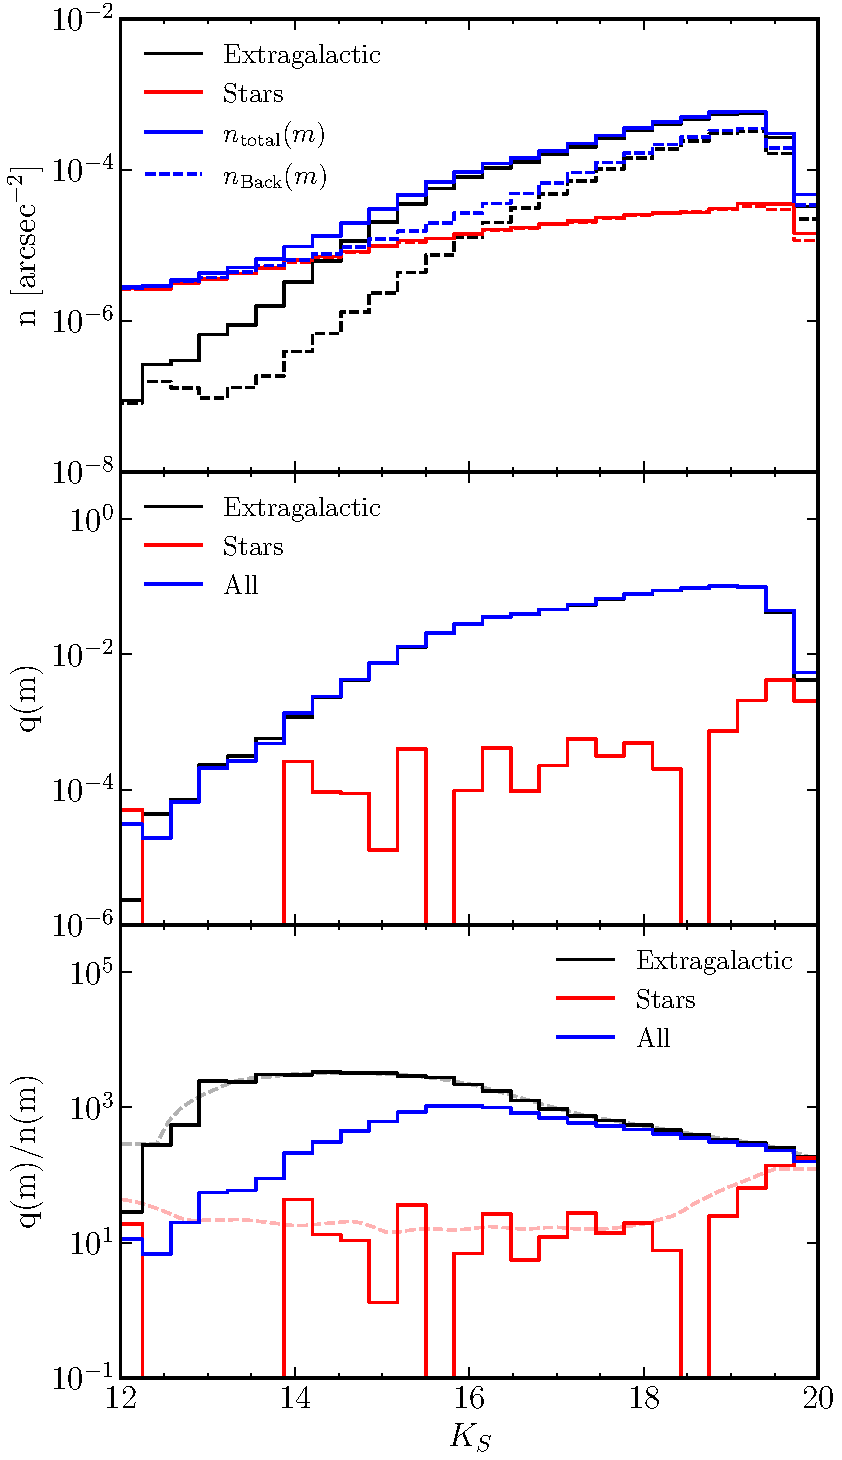
\includegraphics[height=0.75\textheight]{Figures/true_counterparts_distribution.pdf}
	\caption[$K_s$-band distribution of counterparts, separated into galaxies and stars]{Top panel: The $K_s$-band magnitude distributions of objects located within $15\,$arcsec of $250\,\mu$m \textit{Herschel} positions (blue solid line) and random positions (blue dashed line). Each histogram is separated by their extragalactic (black lines) and stellar (red lines) classification. Middle panel: The $K_s$-band magnitude distribution of "true" counterparts accounting for the excess of VIKING sources observed near \textit{Herschel} sources. Bottom panel: The ratio between the "true" counterparts distribution (middle panel) and the background distribution of sources, as used in the calculation of the likelihood ratios in Equation \ref{eq:likelihood_ratio}. The dashed lines represent smoothed fits to $q(m)/n(m)$ to provide a continuous function at all magnitudes. The colour convention of the middle and bottom panels are the same as the top panel.}
	\label{fig:true_counterparts_distribution}
\end{figure}

\subsection{Estimating Q}
\label{sec:estimating_Q}

We predict the probability of finding a genuine counterpart on the VIKING images below the limiting magnitude of the near-IR survey, $Q$, using the method described in \citealt{Fleuren_2012}. While some methods in the literature derive $Q$ directly by summing the $n_{\textrm{real}}(m)$ distribution and dividing by the number of SPIRE sources, this leads to a systematic overestimate due to the possibility of clustering or multiple true counterparts due to source blending. An alternative method by \citealt{Fleuren_2012} calculates an estimate of 1-$Q_0$, the probability of \textit{not} observing a VIKING counterpart, by counting the number of \textit{Herschel} sources without VIKING associations within a given search radius, $r$. These sources will be given the name \textit{blanks}, and has a dependency on search radius, $B(r)$.

Blank sources may be observed in one of several scenarios. Given that the number of cross identifications is limited not by the \textit{Herschel} survey flux limit, but on the depth of the near-IR survey, the most likely reason for observing a blank is that the real ID is fainter than the limiting $K_s$-band magnitude. However, we may also observe a blank if the counterpart lies outside the search radius or if the source is a spurious SPIRE detection.

Even when a \textit{Herschel} source has a candidate on the VIKING images, we may not definitively say that a source is not a blank as we may encounter chance alignments with other near-IR objects close to the same line of sight. Thus, to estimate the true number of blanks, we are reminded that the number of blanks we observe must also account for those that are spuriously identified as not blank. In other words, the number of observed blanks is the number of true blanks minus the number of true blanks that happen to have random VIKING interlopers. If we define the number of observed blanks as $B_{\textrm{obs}}$, the number of true blanks as $B_{\textrm{t}}$ and the number of random interlopers as $N_{\textrm{rand}}$, then

\begin{equation}
    B_{\textrm{obs}} = B_{\textrm{t}} - N_{\textrm{rand}} = B_{\textrm{t}} - B_{\textrm{t}} \times f_{\textrm{rand}},
    \label{eq:observed_blanks}
\end{equation}

\noindent where we have assumed that the number of random interlopers can be estimated from the fraction of positions that have random interlopers, $f_{\textrm{rand}}$. This fraction can itself be estimated from the set of random positions used above to calculate $q(m)$. Using a similar set of notation as before: $B_{\textrm{background}}$ to represent the number of blanks from the catalogue of random positions; $N_{\textrm{background}}$ to represent the total number of random positions and $B'_{\textrm{background}}$ representing the number of random positions for which we observe at least one VIKING counterpart (or "non-blank"), we can estimate $f_{\textrm{rand}}$ as

\begin{equation}
    f_{\textrm{rand}} = \frac{B'_{\textrm{background}}}{N_{\textrm{background}}} = \frac{N_{\textrm{background}} - B_{\textrm{background}}}{N_{\textrm{background}}} = 1 - \frac{B_{\textrm{background}}}{N_{\textrm{background}}}.
\end{equation}

To scale this fraction to the size of the SGP catalogue, the same number of random positions are used as there are \textit{Herschel} $250\,\mu$m positions, such that $f_{\textrm{rand}}$ may be written as

\begin{equation}
    f_{\textrm{rand}} = 1 - \frac{B_{\textrm{background}}}{N_{\textrm{250\,\micron}}}.
\end{equation}

From substitution into Equation \ref{eq:observed_blanks}, we define the fraction of \textit{Herschel} sources that are true blanks (i.e. $B_{\textrm{t}}/N_{\textrm{250\,\micron}}$) as

\begin{equation}
    \frac{B_{\textrm{t}}}{N_{\textrm{250\,\micron}}} = \frac{B_{\textrm{obs}}}{B_{\textrm{background}}}.
    \label{eq:true_blanks}
\end{equation}

In summary, to estimate $1-Q$, we need only to divide the number of observed blank $250\,\mu$m positions by the number of observed blank random positions. It is clear that any estimate of $Q$ using this method depends on the given search radius from the \textit{Herschel} source, $r$, thus we calculate this fraction for a range of radii between $0$ and $15\,$arcsec and model the dependence of $B(r) \equiv 1 - Q$ on the search radius in the same manner as \citealt{Fleuren_2012}.

A \textit{Herschel} source that has no VIKING association within a radius $r$ is either a source whose true counterpart is too faint to be detected by the VIKING survey or lies outside the radius, or both. Assuming that such situations are independent of each other, then the probability of either occurring is given by the conditional probability:

\begin{equation}
\label{eq:blank_probability}
    P(\textrm{Blank}) = P(\textrm{Faint} \cup \textrm{Outside}) = P(\textrm{Faint}) + P(\textrm{Outside}) - P(\textrm{Faint} \cap \textrm{Outside}).
\end{equation}

The first term, the probability that the counterpart is too faint to be detected, is given by $1-Q$, while the probability that the counterpart resides outside the search radius is dependent on the probability distribution of offsets between the counterpart and \textit{Herschel} source, $f(r)$. We assume that the sources in the \textit{Herschel}-ATLAS are point-like on the $250\,\mu$m images and that the errors are equal in RA and declination for radial symmetry. While $f(r)$ naturally depends on the positional errors in both the \textit{Herschel} and near-IR detections, we can assume that the near-IR positional errors are negligible compared to those of SPIRE given that the $1\sigma$ VIKING positional errors are $< 0.2\,$arcsec (\citealt{Fleuren_2012}). For this reason, we use a radially symmetric Gaussian for $f(r)$ with width $\sigma_\textrm{pos}$ corresponding to the typical SPIRE positional error. According to the theory of total probability, the probability that an observable counterpart is detected out to any search radius must equal unity, therefore 

\begin{equation}
    \int_0^\infty 2\pi r'f(r')dr' = 1,
\end{equation}

\noindent which implies that our function $f(r)$ take the form

\begin{equation}
    f(r) = \frac{1}{2\pi\sigma_\textrm{pos}^2}e^{\frac{-r^2}{2\sigma_\textrm{pos}^2}}.
\label{eq:positional_offset_distribution}
\end{equation}

If the probability of observing a counterpart within a radius $r$ is given by

\begin{equation}
    F(r) = \int_0^r 2\pi r'f(r')dr',
\end{equation}

\noindent then P(Outside) in Equation \ref{eq:blank_probability} is given by $1 - F(r)$. Upon substitution we find that the probability of observing a blank source as a function of the search radius can be modelled using the function

\begin{equation}
    B(r) = P(\textrm{Blank}) = (1-Q) + (1-F(r)) - (1-Q)(1-F(r)) = 1 - QF(r).
\label{eq:blanks_model}
\end{equation}

In Figure \ref{fig:Q_estimate} we show the number of blank \textit{Herschel} and blank random positions as a function of the search radius (open squares and circles, respectively) as well as their ratio which is our proxy for $B_{\textrm{t}}/N_{\textrm{250\,\micron}}$ (filled circles, recall Equation \ref{eq:true_blanks}). The best fitting $B(r)$ is illustrated as the black line. Using this method we measure the value of $Q$ to be $0.835\pm0.009$ when considering extragalactic and stellar near-IR sources and $Q = 0.823\pm0.009$ when stellar contaminants are removed. This tells us that for approximately $80\%$ of \textit{Herschel} sources, we observe a near-IR counterpart on the VIKING image that is directly associated with the dust emission.

\begin{figure}
    \centering
	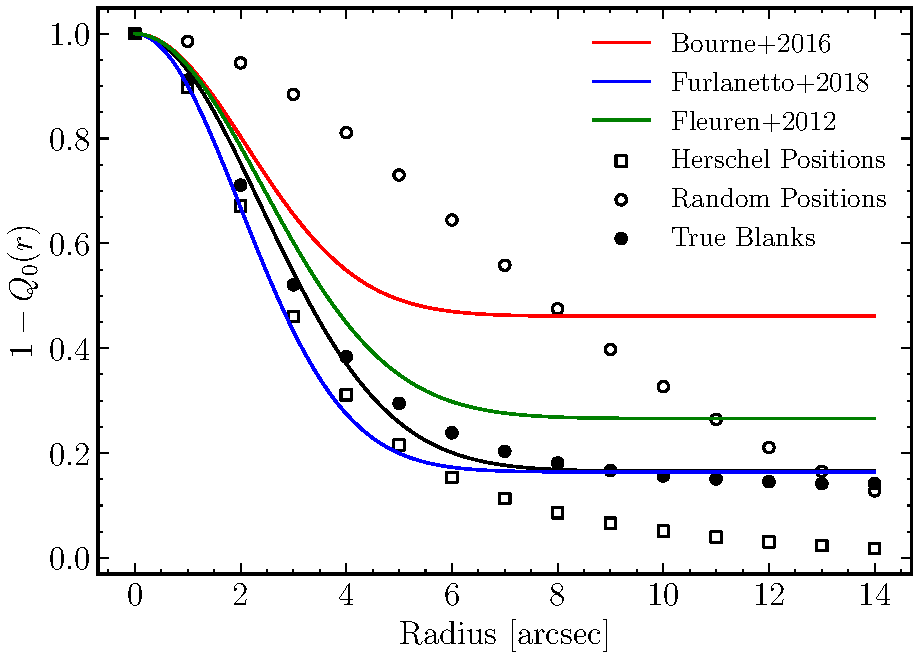
\includegraphics[width=0.67\columnwidth]{Figures/Q_estimate.pdf}
	\caption[An estimate for the number of blank sources as a function of search radius]{Estimates for the number of blanks (sources without VIKING candidates) as a function of the search radius, $r$. Open circles represent the number of blank random positions placed across the SGP field, while open squares represent the number of blank SPIRE $250\,\mu$m positions from H-ATLAS. The filled circles show the division of the two, which acts as our proxy for the fraction of SPIRE sources blank on the VIKING images. The solid black line represents the best fit to the points using Equation \ref{eq:blanks_model}. The same model used in \citealt{Fleuren_2012}, \citealt{Bourne_2016} and \citealt{Furlanetto_2018} are shown as green, red and blue lines respectively.}
	\label{fig:Q_estimate}
\end{figure}

Measurements of the value of $Q$ depend on the depth of the matching survey, and given that the near-IR is less obscured by dust than in the optical (recall Figure \ref{fig:interstellar_medium}), the $Q$ value from studies with optical $r$-band counterparts are typically lower. A comparison of the $Q$ values measured by various \textit{Herschel} studies, and the wavebands that were used, are presented in Table \ref{tab:data_release_input_surveys}.

\begin{table}
\centering
\begin{tabular}{p{3.5cm}|p{3.5cm}|p{2.5cm}|p{3.75cm}}
    \hline
    \hline
    H-ATLAS Release & Input Survey & $Q$ Estimate & Reference \\
    \hline
    \hline
    SDP & $r$ -- SDSS & $0.583$ & \citealt{Smith_2011} \\ 
    Phase 1 GAMA9 & $K_s$ -- VIKING & $0.734\pm0.026$ & \citealt{Fleuren_2012} \\
    Data Release I & $r$ -- SDSS & $0.539\pm0.001$ & \citealt{Bourne_2016} \\
    Data Release II & $r$ -- SDSS & $0.538\pm0.001$ & \citealt{Furlanetto_2018} \\
    Data Release II & $K_s$ -- UKIRT & $0.836\pm0.001$ & \citealt{Furlanetto_2018} \\
    Data Release III & $K_s$ -- VIKING & $0.835\pm0.009$ & This work \\
    \hline
\end{tabular}
\caption[Comparison of optical/near-IR surveys used in H-ATLAS studies]{Comparison of the measured values of $Q$ from \textit{Herschel}-ATLAS studies. From left to right the columns contain: the data release of H-ATLAS; the input survey and the passband used; the fraction of sources with associated counterparts observed on the optical/near-IR images, $Q$; and the reference of the study.}
\label{tab:data_release_input_surveys}
\end{table}

\subsection{Positional Uncertainty of H-ATLAS Detections}

We see from Figure \ref{fig:Q_estimate} that $B(r)$ becomes flat at approximately $3\sigma_{\textrm{pos}}$, suggesting that few counterparts are to be found at search radii greater than $\sim 7\,$arcsec. The function $B(r)$ also provides a prediction for the standard SPIRE positional error, $\sigma_{\textrm{pos}}$, which defines the width of the positional offset distribution $f(r)$. We measure this value to be $\sigma_{\textrm{pos}} = 2.388\pm0.065\,$arcsec. The positional uncertainty has a dependency on the SNR of the far-IR detection (\citealt{Bourne_2016}) and, in theory, should depend on both the full-width at half-maximum (FWHM) of the beam and the SNR following

\begin{equation}
    \sigma_{\textrm{pos}} = 0.6\times\frac{\textrm{FWHM}}{\textrm{SNR}},
\label{eq:positional_uncertainty_theory}
\end{equation}

\noindent as derived in \citealt{Ivison_2007}, on the assumption of uncorrelated noise. However, the addition of confusion noise and clustering of sources have the effect of increasing the prefactor of $0.6$ (\citealt{Chapin_2011}; \citealt{Bourne_2014}). To account for this, a scaling factor (typically about $1.09$, corresponding to a redefined prefactor of $\sim 0.65$) is often applied and is more suitable for sources extracted from far-IR/sub-mm images. To estimate the reliability of each individual counterpart, we require knowing the $1\sigma$ positional uncertainty of each $250\,\mu$m source. To do this, we first make a check on the appropriate prefactor to use in Equation \ref{eq:positional_uncertainty_theory}. Assuming a FWHM of $18\,$arcsec and the fitted value of $\sigma_{\textrm{pos}} = 2.388\,$arcsec, we use the SNR of all $250\,\mu$m sources to obtain a set of values for the prefactor. The median value of this distribution is $0.66$, which we shall use herein. Substituting the prefactor for $0.66$, we estimate $\sigma_{\textrm{pos}}$ for each \textit{Herschel} source, and thus an individual function of $f(r)$ to use when calculating the reliability values.

\section{Likelihood Ratio Results}
\label{sec:lr_results}

We apply Equation \ref{eq:reliability_multiple_counterparts} to all potential near-IR counterparts within $15\,$arcsec of a \textit{Herschel} source. As mentioned previously, the SGP catalogue contains $193,527$ far-IR sources, of which $190,788$ have at least one possible counterpart identified within our search radius. Having matched each source with its highest reliability counterpart we find that $181,373$ ($95.1\%$) are sources with VIKING identifications indicating the source is a galaxy and $9,415$ ($4.9\%$) have stellar classifications. 

In keeping with previous studies, we define reliable matches as those sources with counterparts having $R \geq 0.8$. This provides a balance between minimizing the number of falsely identified counterparts, and ensuring that the sample is not severely contaminated by blended sources. We further justify this choice later in this Section. We identified $111,065$ reliable near-IR counterparts, representing $58.2\%$ of all SGP sources for which there was at least one possible candidate. Of the reliable IDs, $110,374$ ($99.4\%$) are classified as galaxies and $691$ ($0.6\%$) as stellar. The fraction of galaxies is much higher for our "reliable" sample than it is for the whole VIKING catalogue (Section \ref{sec:star_galaxy_classifier}), suggesting that the LR method is highly biased against stars, as is intended. 

On the assumption that a source that is erroneously matched with a counterpart has a probability of $1 - R$, we can estimate the false ID rate for our reliable matches from

\begin{equation}
    N_{\textrm{False}} = \sum_{R_i \geq 0.8} (1 - R_i) = 5,343.
\label{eq:false_ids}
\end{equation}

We predict that there are $5,343$ "false reliable" IDs in the SGP, representing $4.8\%$ of the reliable sample. This can be compared to values of 4.7\% in the GAMA fields and the NGP ($r$-band SDSS matching), 4.5\% for the NGP ($K_s$-band matching) and 4.2\% during the SDP. While the false identification rate for the SGP is in keeping with the other studies, it is the highest value. We might expect that the near-IR analyses would have the lowest false identification rates, as the limiting $K_s$-band magnitude of the VIKING survey corresponds to higher redshift galaxies than the limiting $r$-band magnitude in the SDSS studies. As mentioned earlier, the limiting factor in the number of matches we obtain is in the limits of the optical/near-IR catalogue, not the far-IR survey. This leaves many \textit{Herschel} sources at high redshift that do not get matched to any counterpart, or possibly, erroneously matched to a much lower redshift counterpart. This problem would be greater for the optical surveys, and thus they would have a higher false ID rate. However, in our analysis of the SGP, we chose to use an increased search radius of $15\,$arcsec (compared to $10\,$arcsec in other H-ATLAS studies). We chose the larger radius to avoid missing any unusual VIKING associations, such as those that might lie at larger $r$ due to the effects of gravitational lensing. As shown in \citealt{Bakx_2020}, there are still genuine associations observed on the VIKING images beyond $10\,$arcsec, and we wish to retain these in our catalogue despite them being unlikely to have significant reliability values. The result is that the average number of potential candidates increases per source, and given that the LR method requires that the sum of all candidates' reliabilities add to one, the average reliability of the true ID will fall, leading to a higher false identification rate. Further discussion on the effect of increasing the search radius is made in Section \ref{sec:multiplicity}.

The completeness, $\eta$, of the reliable sample is defined as the fraction of \textit{Herschel} sources that are recovered with a reliability greater than $0.8$ (\citealt{Smith_2011}) and can be calculated as

\begin{equation}
    \eta = \frac{n(R \geq 0.8)}{n(\textrm{SNR}_{250} \geq 4) \times Q},
\label{eq:completeness}
\end{equation}

\noindent where the numerator is the size of the reliable sample and the denominator predicts the true number of sources. As would be expected, a value of $\eta = 1$ would imply that the fraction of all counterparts deemed reliable has reached its theoretical maximum, $Q$. Another important test of our sample is the cleanness, $C$, an estimate of the number of sources that are not spurious matches, given by

\begin{equation}
    C = 1 - \frac{N_{\textrm{False}}}{N_{\textrm{250\,\micron}}}.
\label{eq:cleanness}
\end{equation}

At a minimum reliability cut of $0.8$, we find that the completeness of the reliable galaxy sample is $\eta = 78\%$, which is similar to the completeness values found for the NGP and GAMA fields of $74\%$ and $73\%$, respectively. Figure \ref{fig:completeness_and_cleanness} shows how the completeness and cleanness change for a range of different reliability thresholds. We see that a cut at $R \geq 0.8$ selects a highly clean sample at a minor expense in completeness. While an increase in the reliability cut would yield a marginally cleaner sample, it would be offset drastically by a fall in completeness. A decrease in the minimum reliability would lead to an increase in completeness, with only a small decrease in cleanness, but reducing the threshold too far would also lead to problems securing a one-to-one matching between \textit{Herschel} sources and counterparts. At $R \geq 0.8$ we set a minimum value that is a good balance between the two values.

\begin{figure}
    \centering
	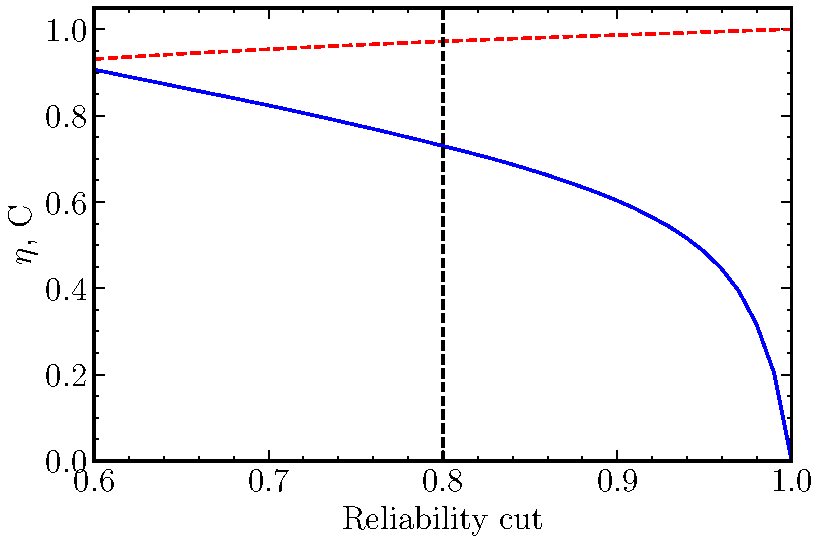
\includegraphics[width=0.8\columnwidth]{Figures/completeness_and_cleanness.pdf}
	\caption[Completeness and cleanness of the SGP sample as a function of reliabilty]{The completeness, $\eta$, and cleanness, $C$, of the SGP sample as a function of various minimum reliability values, illustrated as solid blue and red dashed lines, respectively. The vertical dashed line reprents the minimum reliability cut used in all H-ATLAS studies ($R \geq 0.8$).}
	\label{fig:completeness_and_cleanness}
\end{figure}

\section{Multiplicity of Counterparts}
\label{sec:multiplicity}

One disadvantage of using the LR method to identify counterparts to low resolution sources is that it assumes a one-to-one matching of source and counterpart. Given that the sum of reliabilities of all possible counterparts may not exceed one, we have a bias against \textit{Herschel} sources with many candidates, the result of merging galaxies, members of groups and clusters, and non-physical associations such as confusion due to blending. The combined reliabilities of multiple systems reduces the maximum reliability of the single chosen ID. For example, consider two galaxies in a cluster that are both observed on the VIKING images close to the \textit{Herschel} position. It is reasonable to imagine that these two objects may have similar $K_s$-band magnitudes and radial offsets and, if they are close to the position of the far-IR emission, may both have high likelihoods. In such a case, either source may be considered the true ID to the source (and in reality both are likely associated), but the use of Equation \ref{eq:reliability_multiple_counterparts} to measure their reliabilities leads to the following, 

\begin{equation}
    R_j \sim \frac{L_j}{\sum_i L_i} \sim \frac{L_j}{2L_j} \sim 0.5.
\end{equation}

In this scenario, neither counterpart would be considered the true ID and thus we generate a bias against multiple systems in our catalogue. Table \ref{tab:multiplicity} shows the fraction of \textit{Herschel} sources that have reliable identifications, which decreases as a function of the number of possible counterparts. This would suggest that the sample is partly incomplete because we miss sources where there are more than one genuine association on the VIKING image. In Figure \ref{fig:multiplicity} we show this reliable fraction as a function of multiplicity compared with previous H-ATLAS studies. Compared to the Science Demonstration Phase (\citealt{Fleuren_2012}), GAMA fields (\citealt{Bourne_2016}) and the NGP (\citealt{Furlanetto_2018}), we see that the SGP reliability fraction declines more slowly, peaks at higher average $N_{\textrm{Match}}$ and is slightly lower for sources where there is only a single possible counterpart. All these differences may be explained by the increased search radius. The increase from $10\,$arcsec to $15\,$arcsec is a significant change as it equates to more than double the total area of the near-IR image ($A_{\textrm{SGP}}/A_{\textrm{Other}} = \pi r_{\textrm{SGP}}^2/\pi r_{\textrm{Other}}^2 = 225\pi/100\pi = 2.25$). While the increased $r$ means that we are more likely to observe a reliable counterpart, it also increases the probability of matching erroneously with a background galaxy, thus the low fraction at $N_{\textrm{Match}} = 1$ may be due to an increase in unassociated VIKING objects being selected as the true identification. In Table \ref{tab:multiplicity} we see that the average offset between the VIKING galaxy and \textit{Herschel} source is substantially higher when the galaxy is the only possible candidate, suggesting that some fraction of these sources are erroneously matched. Occasionally, our chosen reliable ID will be unassociated with the \textit{Herschel} source, but selected for being the only observed counterpart. This is more likely to happen when there is only one candidate (and in reality the source is blank on the near-IR image), resulting in the jump in the average separation. Another reason why the reliable fraction is low for $N_{\textrm{Match}} = 1$ is that a large fraction of the stellar candidates will fall in this bin as stars tend to be isolated (\citealt{Bourne_2016}). The shift in the peak is likely due to the greater ability to discern between true IDs and background interlopers when $N_{\textrm{Match}}$ candidates are spread over double the area.

\begin{table}
    \centering
    \begin{tabular}{p{2cm}|p{2cm}|p{2cm}|p{2cm}|p{4cm}}
        \hline
        \hline
        $N_{\textrm{Match}}$ & $N_{\textrm{SPIRE}}$ & $N_{\textrm{Reliable}}$ & Percent & Av. Separation [arcsec] \\
        \hline
        \hline
        0 & 2,739 & 0 & 0 & 0 \\
        1 & 11,692 & 5,477 & 47 & 6.3 \\
        2 & 24,268 & 14,568 & 60 & 4.7 \\
        3 & 32,948 & 20,396 & 62 & 4.1 \\
        4 & 33,526 & 20,383 & 61 & 3.8 \\
        5 & 27,745 & 16,359 & 59 & 3.6 \\
        6 & 20,236 & 11,563 & 57 & 3.4 \\
        7 & 12,999 & 7,155 & 55 & 3.4 \\
        8 & 8,079 & 4,355 & 54 & 3.3 \\
        9 & 4,983 & 2,640 & 53 & 3.4 \\
        10 & 3,017 & 1,643 & 54 & 3.3 \\
        \hline
    \end{tabular}
    \caption[Reliable fraction of SGP sources as a function of the number of candidates]{The reliable fraction as a function of the number of candidates observed per source. From left to right the columns contain: the number of observed candidates per source; the number of \textit{Herschel} sources that have $N_{\textrm{Match}}$ candidates; the number of those sources whose best counterpart has a reliability greater than $0.8$; the reliable fraction given as a percentage; and the average separation between the chosen ID and the \textit{Herschel} source in arcsec.}
    \label{tab:multiplicity}
\end{table}

\begin{figure}
    \centering
    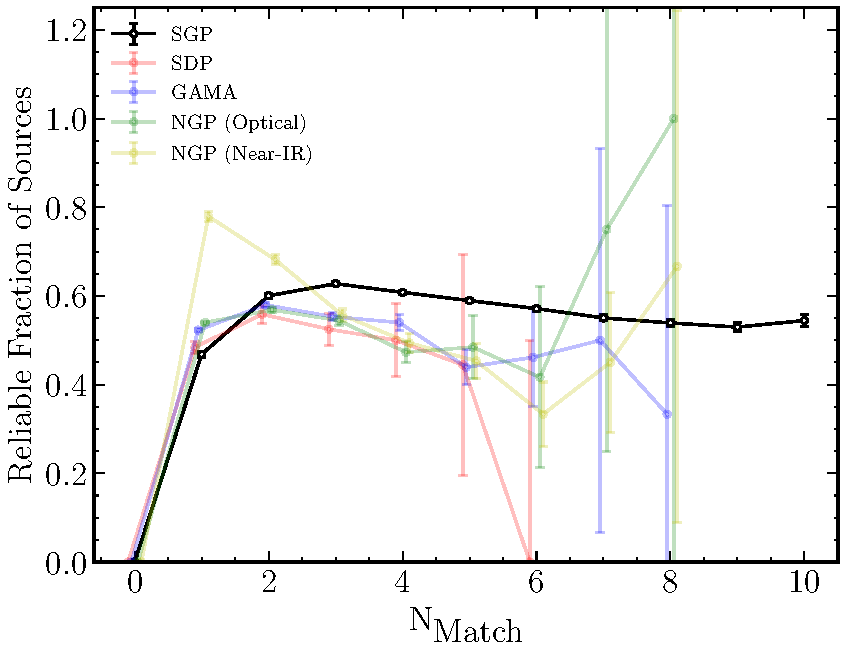
\includegraphics[width=0.67\columnwidth]{Figures/multiplicity.pdf}
    \caption[Reliable fraction of sources as a function of the number of candidates]{The fraction of \textit{Herschel} sources with reliably matched counterparts as a function of the number of observed candidates. The results from various H-ATLAS studies are shown with the following lines: SGP (black, this work), SDP (red, \citealt{Smith_2011}), GAMA (blue, \citealt{Bourne_2016}) and NGP (optical in green and near-IR in yellow, \citealt{Furlanetto_2018}). All other works used a maximum search radius of $10\,$arcsec while the SGP analysis used $15\,$arcsec. For clarity each line has been offset in $N_{\textrm{Match}}$ by a different value.}
    \label{fig:multiplicity}
\end{figure}

One way we can predict the number of \textit{Herschel} sources that are missed by the LR method due to multiple genuine counterparts, is by assuming that all candidates are true associations if their combined reliability is greater than $0.8$, but where no individual object reaches this threshold. However, in our case of large $r$, even moderately valued $R$ counterparts will combine to exceed this minimum reliability. Alternatively, we may consider the likelihood values of each counterpart, which, unlike their reliability values, do not have an upper bound. From Equation \ref{eq:reliability_multiple_counterparts} we see that a reliability of $0.8$ or greater corresponds to $L > 0.66$, assuming a single candidate and a value of $Q = 0.835$. An alternative estimate for the number of lost sources can then be made assuming that a source with a matched counterpart with $L > 0.66$ but $R < 0.8$ is likely influenced by nearby candidates. We find $33,967$ \textit{Herschel} sources that satisfy these conditions. We expect that this number is still overestimated, however, as it will include chance alignments. A more realistic number of sources with two or more physically associated counterparts requires knowing their redshifts.

As shown in \citealt{Fleuren_2012}, chance alignments along the line of sight can be ruled out by comparing the redshifts of the VIKING galaxies. They propose that associated galaxies have photometric redshifts within $\sim 10\%$ of each other, while spectroscopic redshifts fall within $\sim 5\%$. Other than catastrophic redshifts, the only other scenario in which this method fails is if the \textit{Herschel} source lies on a similar line of sight to unrelated groups or merging galaxies. In the following, we describe a new method for estimating the number of missed \textit{Herschel} sources that compares the redshifts of our VIKING counterparts with the redshifts of background galaxies. The photometric redshifts that are used in this section are described in detail in Section \ref{sec:phot_z_VIKING}.

Firstly, we restrict both the SGP near-IR counterpart catalogue and the background catalogue (from Section \ref{sec:true_counterparts_distribution}) to contain only sources with two or more counterparts. We then restrict this further to counterparts found within $8\,$arcsec of the source (or random) position. This second selection reduces the samples to likelihood ratios above $\sim 0.66$, reducing the chance of observing unrelated galaxies. For all source positions we identify the pair of galaxies with the closest redshifts and measure the quantity $\Delta z/\sigma_{\Delta z}$, the difference in redshift divided by the error in their separation. In Figure \ref{fig:delta_z_multiplicity} we show the probability distribution functions (PDFs) of $\Delta z/\sigma_{\Delta z}$ for the SGP catalogue (red line) and the background catalogue (black line). A subtraction of the latter from the former gives an excess close to $\Delta z = 0$ (blue line). The area of this peak represents the probability that a close pair of VIKING galaxies are indeed related to the \textit{Herschel} source. We fit a Gaussian profile to this excess and estimate this probability to be $2 - 5\%$. After multiplying this probability by the number of \textit{Herschel} sources where we observe a close pair of VIKING galaxies (which we shall define as having $-0.1 < \Delta z/\sigma_{\Delta z} < 0.1$), then we find an estimate for the number of \textit{Herschel} sources with genuine multiple counterparts of $\sim 400 - 1,000$.

\begin{figure}
    \centering
    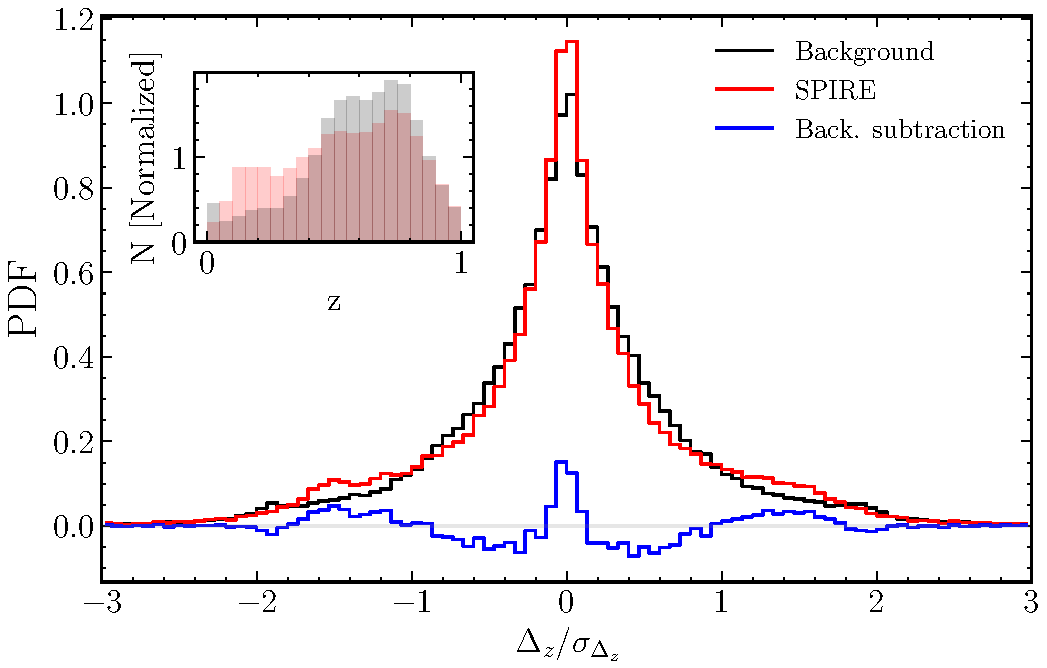
\includegraphics[width=0.8\columnwidth]{Figures/delta_z_multiplicity.pdf}
    \caption[PDFs of $\Delta z/\sigma_{\Delta z}$ for \textit{Herschel} sources and random positions]{Probability distribution functions for the quantity $\Delta z/\sigma_{\Delta z}$, the difference in photometric redshifts divided by the error on this value. This quantity is calculated for pairs of VIKING galaxies located within $8\,$arcsec of a \textit{Herschel} position (red histogram) and random positions (black histogram). The blue histogram represents a background subtraction of the former. The excess located at $\Delta z = 0$ represents the probability that a pair of VIKING counterparts with similar redshifts are associated with the \textit{Herschel} source. The inset figure shows the normalized redshift distribution of counterparts observed within $8\,$arcsec of the $250\,\mu$m positions in red and random positions in grey.}
    \label{fig:delta_z_multiplicity}
\end{figure}

It should be noted that this method is independent of the LR method, and so the closest redshift pair may not always contain the counterpart with the highest reliability. In total we observe $70,880$ sources with pairs of near-IR counterparts at similar redshifts, but only three quarters of these contain our chosen identification. The remaining quarter of sources may be located along the same line of sight as unrelated galaxy interactions, or the multiple system is related to the \textit{Herschel} source, but is overlooked by the one-to-one matching of the LR technique. The subset of sources in this method represents approximately one third of the whole SGP catalogue ($70,880/193,527$), and so we expect many more galaxy groups and mergers to be in the full SGP survey. Moreover, there is evidence to suggest that the merger rate of galaxies evolves with redshift, and peaks at $z \sim 1$ (e.g. \citealt{Bell_2006, Ryan_2008}). If true, then a large fraction of the interacting systems in the SGP may be beyond the detection limit of the VIKING survey, and are the cause of some of the blank fields.

\section{Photometric Redshifts}

\subsection{Redshifts of the \textit{Herschel} Sources}
\label{sec:phot_z_Herschel}

Any study on the evolution of the properties of galaxies requires knowing its redshift. With far-IR sources and their near-IR counterparts, we can begin to construct SEDs that constrain both the stellar and dust emission. The far-IR spectra of \textit{Herschel} galaxies are well described by a two-temperature modified blackbody model, as presented in \citealt{Pearson_2013}. This model takes the form 

\begin{equation}
    S_\nu = A[B_\nu(T_{\textrm{hot}})\nu^\beta + \alpha B_\nu(T_{\textrm{cold}})\nu^\beta],
\label{eq:pearson_sed_model}
\end{equation}

\noindent where $S_\nu$ is the flux density of the source at the rest frame frequency, $\nu$, $A$ is a normalization factor, $B(T)$ represents the Planck function at temperature $T$ (here we assume two dust temperatures, $T_{\textrm{hot}}$ and $T_{\textrm{cold}}$), $\beta$ is the dust emissivity index and $\alpha$ represents the fraction of cold dust mass to hot dust mass. Using a sample of $40$ H-ATLAS sources with spectroscopic redshifts, \citealt{Pearson_2013} found that the best fitting set of parameters were $T_{\textrm{hot}} = 46.9\,$K, $T_{\textrm{cold}} = 23.9\,$K and $\alpha = 30.1$ (assuming a fixed value of $\beta = 2$). Assuming these fixed values, we define the model given by Equation \ref{eq:pearson_sed_model} with just two free parameters, the overall normalization and the redshift of the galaxy. We use this model to determine the photometric redshifts of our galaxies directly from the dust emission. It is a useful model to apply to our SGP sample as we have few \textit{Herschel} observations with which to constrain the far-IR SED and therefore cannot use a model with many parameters. For each source the normalization and redshift were varied until the following $\chi^2$ reached a minimum:

\begin{equation}
    \chi^2 = \sum_i \frac{(S_i - S_{i,m})^2}{E_i^2}.
    \label{eq:chi_squared}
\end{equation}

$S_i$ represents the flux density at each \textit{Herschel} wavelength, $i$, $S_{i,m}$ is the model prediction of the flux and $E_i$ is the flux density error. As discussed in Section \ref{sec:Detecting Submillimeter Sources on Herschel Images}, the \textit{Herschel} sources in DR2 have flux density errors obtained from images including instrumental and confusion noise, but they do not contain a calibration error. The calibration error is formed of two parts: i) the main contribution comes from the uncertainty in imaging a set of calibration objects, which in the case of SPIRE is Neptune and for PACS is a group of stars and asteroids. This error is correlated between the bands and is approximately $4\%$ for SPIRE; and ii) a contribution uncorrelated between bands of $1.5\%$ (\citealt{Valiante_2016}). While the correlated error scales all fluxes by the same amount, and therefore does not impact on the $\chi^2$, the uncorrelated errors do contribute and are calculated by adding in quadrature the errors in the DR2 catalogue with the errors obtained by multiplying the flux density of each source by $1.5\%$ such that $\bar{E_i} = \sqrt{E_i^2 + (S_i \times 0.015)^2}$, where $\bar{E_i}$ is the new, calibration included error and replaces $E_i$ in Equation \ref{eq:chi_squared}.

The $1\sigma$ errors on our photometric redshifts were taken to be the range above and below the best-fitting value where the $\chi^2$ increases by one. When taking all sources collectively, the mean reduced $\chi^2$ ($\chi_\nu^2 = \chi^2/\nu$ where $\nu$ is the number of degrees of freedom) should have a value of $\sim 1$ if the model sufficiently represents the data. A mean value of $\chi_\nu^2 > 1$ would suggest that the model is not a good representation of the data, while a mean value $\chi_\nu^2 < 1$ implies that either the model has too many free parameters or that the errors on the data are too large. The $\chi^2$-minimization applied to the sources in the SGP yields a mean value of $\chi_\nu^2 = 0.55$. Given that the model requires only two free parameters, it is more likely that this low value is a result of overestimated flux uncertainties. While the errors on the photometric redshifts account for all relevant uncertainties in the flux densities, it does not account for uncertainty in the model SED of \citealt{Pearson_2013}, especially given that high-redshift \textit{Herschel} galaxies have been shown to have a variety of SED shapes (\citealt{Bakx_2018}). The H-ATLAS sources used to generate the characteristic SED of \citealt{Pearson_2013} are intrinsically bright (facilitating their spectroscopic redshift search) and thus have fractionally smaller errors on their flux densities than the full H-ATLAS sample. This results in errors in the photometric redshifts smaller than appropriate for the wide variety of sources observed in H-ATLAS. For this reason, the redshift error estimated by \citealt{Pearson_2013}, $\Delta z/(1+z) = 0.12$, should represent a minimum redshift error that is caused by the diversity of real galaxy SEDs, and should be taken as a minimum value when applied to the SGP data. For $\sim 9\%$ of sources the measured redshift error is lower than this minimum value and we have therefore replaced the redshift error from the SED fitting with $\Delta z/(1+z) = 0.12$. The median redshift of the \textit{Herschel} sources in the SGP is $\sim 1.4$ and has a peak at a similar value. More than $100$ \textit{Herschel} galaxies have $z > 5$. The distribution of photometric redshifts can be seen in Figure \ref{fig:redshift_distribution} in blue.

\subsection{Redshifts of the VIKING Counterparts}
\label{sec:phot_z_VIKING}

We obtain photometric redshifts for the VIKING counterparts by matching the catalogue to the \textit{Herschel} Extragalactic Legacy Project (HELP; \citealt{Vaccari_2016, Shirley_2019}). HELP provides an extensive catalogue of extragalactic sources observed across \textit{Herschel} surveys. The photometric redshifts in HELP are based on the template-fitting method of \citealt{Duncan_2018a} and the machine learning method of \citealt{Duncan_2018b}.

The approach combines the redshift posterior distributions from template fitting with those from machine learning to generate a final distribution from their Bayesian combination. Three different sets of templates were used: the default library of SEDs provided with the photometric redshift code \texttt{EAZY} (\citealt{Brammer_2008}); the XMM-COSMOS templates of \citealt{Salvato_2009} and \citealt{Salvato_2011}, which cover a wide range of galaxy spectral types including active galactic nuclei (AGN) and QSO templates; and the atlas of galaxy SEDs presented in \citealt{Brown_2014}, a set of 129 galaxy SED templates based on a range of nearby galaxies including ellipticals, spirals and luminous IR galaxies. The machine learning algorithm uses a training set compiled from a sample of $48,995$ galaxies with spectroscopic redshifts in the SGP plus further redshifts from the three GAMA fields (the surveys used in the training set include the 2dF, 6dF, 2MRS and SRSS2 surveys). Three separate redshift estimates were made using three sets of filters: $u$, $g$, $r$ and $i$ from OmegaCAM on the VLT Survey Telescope; $g$, $r$, $i$, $z$ and $y$ from the Dark Energy Camera (DECam) on the Victor M. Blanco 4-meter Telescope; and $J$ and $K_s$ from the VISTA InfraRed CAMera (VIRCAM) on VISTA, along with the aforementioned $g$, $r$ and $i$ bands from OmegaCam. The machine learning redshifts were generated using the redshift code GPz (\citealt{Almosallam_2016}). The template and machine learning derived redshift posteriors were then combined using the Hierarchical Bayesian combination method described in \citealt{Dahlen_2013} to generate a single redshift posterior for each HELP galaxy.

The redshift of the counterparts are taken from the full posterior distribution in the following way. First, an 80\% highest probability density (HPD) credible interval (CI) was calculated by starting at the peak redshift probability and lowering a threshold until 80\% of the total probability lies above the line. The resulting HPD CI may have two or more peaks, in such cases they are ranked from the most to least probable based on their peak value. The redshift is assumed to be the median of the primary peak. Next, to estimate the errors on the redshift, we assumed that the upper and lower boundaries of the primary peak defines a Gaussian, symmetric about some mean redshift close to the median redshift. We thus transform the $80\%$ credible interval into $1\sigma$ errors assuming a Gaussian distribution where an $80\%$ CI is equal to $1.282\sigma$.

In total there are $29,790,690$ objects with photometric redshifts in the HELP catalogue of the SGP field. We use a $0.5\,$arcsec matching radius to find the nearest neighbour to all the VIKING counterparts. This yields $542,302$ ($54\%$) redshifts, corresponding to $82,195$ ($74\%$) sources in our reliable SGP sample. Given the limiting magnitude of the VIKING survey, most counterparts have $z < 1$. This covers only a fraction of all \textit{Herschel} sources in the SGP, but does improve on the redshifts reached by the SDSS, which have very few galaxies beyond $z \sim 0.5$. The distribution of redshifts for the VIKING counterparts can be seen in Figure \ref{fig:redshift_distribution} in red. The median uncertainty on the counterpart redshift is $\sim 0.21$, while the far-IR sources have redshifts with uncertainties $\sim 0.51$. Thus, to derive the most accurate photometric redshift distribution of the \textit{Herschel} sources, we preferentially chose to use the redshift of the counterpart, and failing this, use the redshift estimated from \textit{Herschel} fluxes. This optimal distribution is shown in black in the same figure.

\begin{figure}
    \centering
    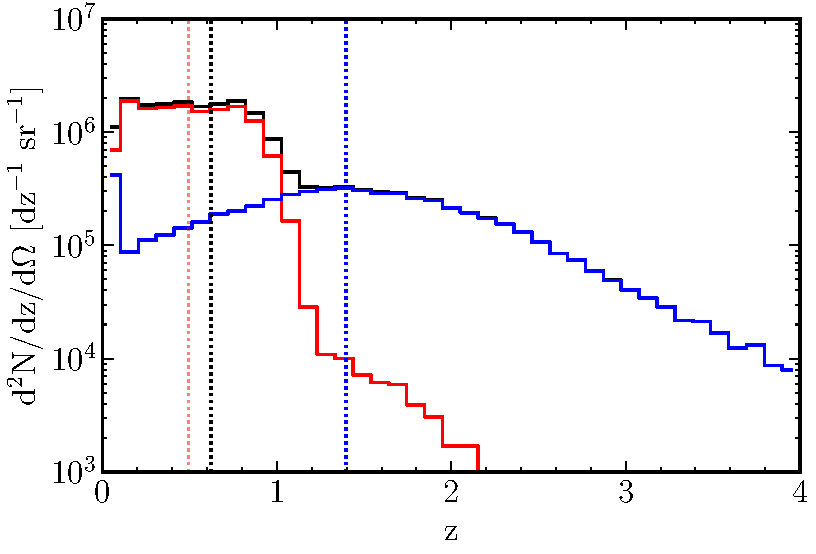
\includegraphics[width=0.8\columnwidth]{Figures/redshift_distribution.pdf}
    \caption[Photometric redshift distribution of SGP sources]{Photometric redshift distribution of the sources in the SGP field of H-ATLAS. The blue line represents the distribution of redshifts obtained from the SED fitting of the far-IR flux densities; the red line represents the distribution of redshifts for the near-infrared counterparts, as matched with the \textit{Herschel} Extragalactic Legacy Project; and the black line represents the distribution of the best estimate for each source, preferentially selecting the redshift of the counterpart. The median redshifts are $z_{\textrm{far-IR}} = 1.40$, $z_{\textrm{near-IR}} = 0.49$ and $z_{\textrm{best}} = 0.62$ and are illustrated by the dotted red, blue and black vertical lines respectively.}
    \label{fig:redshift_distribution}
\end{figure}

\section{Gravitational Lensing in the SGP}

When the light from a distant galaxy is close to the same line of sight as a foreground mass, whether that be an individual galaxy (likely a massive elliptical) or galaxy cluster, the magnification of the background source due to the deflection of the light makes the galaxy appear brighter with a larger angular size. This effect, known as gravitational lensing, makes these systems ideal targets for studying intrinsically faint and distant galaxies that may otherwise be impossible to observe. This effect can be exploited to generate a sample of prime targets for certain studies, such as investigating the physical conditions in distant star forming galaxies, measurement of the cosmological parameters (e.g. \citealt{Kochanek_1992, Kochanek_1996, Grillo_2008, Oguri_2012, Eales_2015}) and the evolution of the equation of state of dark matter (e.g. \citealt{Zhang_2009}). 

Identifying the signs of gravitational lensing (e.g. Einstein rings) from follow up imaging can be very time-consuming and not practical for large surveys. However, wide area, blank field far-IR surveys have been shown to contain a vast number of lensing events, that can be easily detected from their bright far-IR emission (e.g. \citealt{Blain_1996, Perrotta_2002, Negrello_2007, Paciga_2009, Bakx_2020}). The source counts of unlensed (by which we mean not lensed) \textit{Herschel} galaxies falls dramatically at high flux densities ($S_{500} \gtrsim 100\,$mJy), leaving a population of galaxies that are either at low redshift, bright radio galaxies, or lensed candidates. We can remove the former populations from shallow optical and radio surveys, providing a flux limited sample of far-IR sources with a high likelihood of being lensed, and low contamination. This method has been used many times in previous studies of \textit{Herschel} surveys. \citealt{Negrello_2010} produced the first sample of strongly lensed \textit{Herschel} galaxies (SLGs), presenting $5$ lensed galaxies within the SDP. This was followed by the study of \citealt{Wardlow_2013} that identified $13$ lensed galaxies from HerMES. \citealt{Nayyeri_2016} presented a further $77$ candidates from the $372\,$deg$^2$ of sky covered by the HerMES Large Mode Survey (HeLMS) and the \textit{Herschel} Stripe 82 Survey (HerS; \citealt{Viero_2014}). More recently, \citealt{Negrello_2017} identified a sample of $80$ candidates for lensing from $\sim 600\,$deg$^2$ of the H-ATLAS. In the subsequent sections we shall present a statistical sample of candidate lensed sources from the SGP, first by selecting the brightest sources using the method outlined in \citealt{Negrello_2017}, then extending this to lower flux densities by predicting the likelihood of gravitational lensing based on the redshift distributions of the far-IR sources and their near-IR counterparts. 

\subsection{The Brightest Lensed Sources}
\label{sec:brightest_lenses}

The number counts of unlensed sources falls rapidly at $500\,\mu$m flux densities above $\sim 100\,$mJy because of the steep luminosity function of far-IR selected galaxies. For a given luminosity, the probability of a galaxy having an intrinsic brightness of such high flux density becomes much lower than the probability that an intrinsically fainter source is being magnified due to gravitational lensing. Selecting all sources in the SGP with $S_{500} > 100\,$mJy we find $179$ sources, $175$ of which had at least one observed VIKING counterpart. 

The low-redshift spirals and flat spectrum radio galaxies that contaminate this sample were identified and removed by searching the location of the sources with the NASA/IPAC Extragalactic Database (NED). We also removed two variable stars (HATLASJ012658.0-323234 -- R Sculptoris and HATLASJ225519.6-293644 -- V Piscis Austrini) and five blazars, as listed in Table \ref{tab:blazars}. In total 131 local galaxies were identified from their resolved image in NED and thus removed. Their locality can be inferred from a far-IR colour-colour plot. These objects have much "bluer" far-IR colours than the remaining sample (Figure \ref{fig:submm_colours_lensed_candidates}), suggesting that despite their equally high flux density, they are separate populations at different redshifts. The remaining $41$ sources with "redder" colours, and thus most likely to be at high redshifts, were retained and form our bright lensing candidates. The complete sample of sources is tabulated in Appendix \ref{app:candidate_lenses_bright}. The colour-colour plot shown in Figure \ref{fig:submm_colours_lensed_candidates} illustrates how a relatively clean sample of lensed candidates (barring possible blazars) can be obtained from far-IR/sub-mm fluxes alone.

\begin{table}
    \centering
    \begin{tabular}{p{3.75cm}|p{3.25cm}|p{2cm}|p{2cm}|p{2cm}}
        \hline
        \hline
        H-ATLAS IAU Name & NED Identification & $S_{\textrm{250\,\micron}}$ [mJy] & $S_{\textrm{350\,\micron}}$ [mJy] & $S_{\textrm{500\,\micron}}$ [mJy] \\
        \hline
        \hline
        J014310.0-320056 & PKS 0140-322 & 96.0$\pm$7.5 & 119.5$\pm$8.4 & 122.4$\pm$9.0 \\
        J014503.4-273333 & [HB89] 0142-278 & 131.4$\pm$7.8 & 179.2$\pm$8.8 & 234.4$\pm$9.0 \\
        J222321.6-313701 & PKS 2220-318 & 86.0$\pm$9.5 & 110.9$\pm$10.5 & 131.9$\pm$11.7 \\
        J224838.6-323551 & [HB89] 2245-328 & 119.2$\pm$7.7 & 152.8$\pm$8.3 & 194.7$\pm$8.6 \\
        J235347.4-303746 & PKS 2351-309 & 77.1$\pm$7.4 & 96.6$\pm$8.4 & 103.1$\pm$8.9 \\
        \hline
    \end{tabular}
    \caption[Blazars in the SGP with $S_{500} > 100\,$mJy]{The blazars with $500\,\mu$m flux density $> 100\,$mJy identified in the SGP using NED.}
    \label{tab:blazars}
\end{table}

\begin{figure}
    \centering
    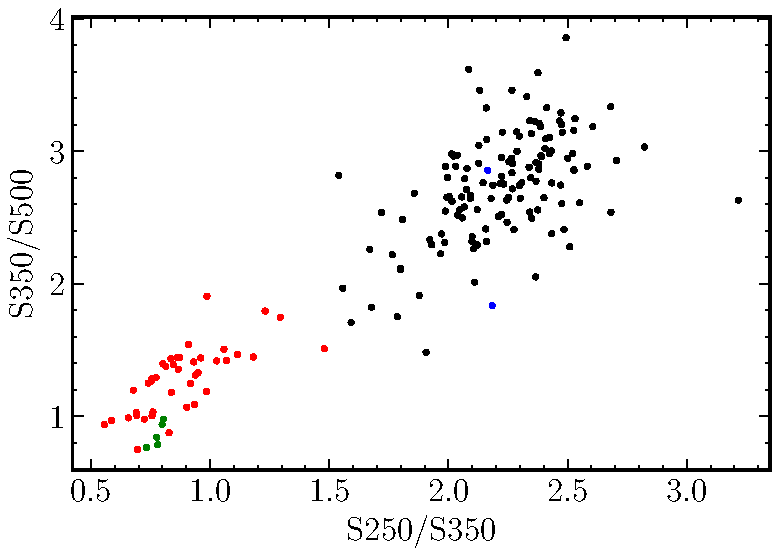
\includegraphics[width=0.8\columnwidth]{Figures/submm_colours_lensed_candidates.pdf}
    \caption[$S_{250}/S_{350}$ against $S_{350}/S_{500}$ diagram of SGP sources with $S_{500} > 100\,$mJy]{A colour-colour diagram ($S_{250}/S_{350}$ against $S_{350}/S_{500}$) for objects with $S_{500} > 100\,$mJy in the SGP. Sources are coloured according to their classification: local galaxies (black), variable stars (blue), blazars (green) and the remaining sources that we take as our candidates for lensing events (red).}
    \label{fig:submm_colours_lensed_candidates}
\end{figure}

The 41 bright candidates include $30$ that were previously identified in \citealt{Negrello_2017}. The $11$ additional sources fall outside of the mask of the SGP used in \citealt{Negrello_2017}. The mask was used to remove the edges of the survey area covered by fewer scans from the SPIRE instrument and thus were affected by higher noise. While the method described here only goes as far as to suggest that these \textit{Herschel} sources are at high redshift, at the time of publication of \citealt{Negrello_2017}, optical to near-IR imaging had only discounted one source from the initial sample for not being strongly lensed. The studies mentioned previously predict that the surface density of SLGs above $100\,$mJy at $500\,\mu$m is $\sim 0.1 - 0.2\,$deg$^{-2}$ (\citealt{Vieira_2010, Wardlow_2013, Nayyeri_2016}). Assuming that all $41$ sources in the SGP are being lensed, the surface density of lensed sources is $0.14\,$deg$^{-2}$. It is interesting to note that two sources with $S_{500} > 100\,$mJy have no VIKING counterpart within $15\,$arcsec and a further $13$ do not have photometric redshifts from HELP. These bright systems may be interesting examples of sources where the lens is at a high redshift (beyond $z \sim 1$), sources that are lensed by a cluster, or not being lensed at all.

\subsection{Extending the Search for Lenses to Lower Fluxes}

While selecting the brightest \textit{Herschel} sources is an easy and effective method for sampling those with the highest probability of lensing, the chance of a \textit{Herschel} source being lensed need not be dependent on its intrinsic brightness and many lensing events are missed because their magnification factors do not substantially lift their fluxes above the level of other, more intrinsically bright unlensed sources. An alternative way to predict the probability that a source is lensed is to compare the redshifts of the near-IR counterparts and the dust emitting source. On the assumption that the counterpart is not the true identification for the galaxy, but rather a foreground deflector, the redshift of the counterpart would be much lower than the redshift of the \textit{Herschel} galaxy.

Comparing the properties of \textit{Herschel} sources and their counterparts has already been used in previous studies to predict gravitational lensing events; a notable example of this being the Statistical \textit{Herschel}-ATLAS Lensed Objects Selection (SHALOS; \citealt{Gonzalez-Nuevo_2019}) which was used to predict that there are several hundred SLG candidates in the GAMA and NGP fields. In \citealt{Gonzalez-Nuevo_2019} these properties include their redshifts (the greater the disparity the higher the probability); the angular separation of the source and object (the closer to the same line of sight the higher the probability); the ratio between the optical and \textit{Herschel} flux densities; and the luminosity of the source compared to other galaxies at similar redshifts. For simplicity we implement a comparison of their redshifts only. The reason for this is two-fold. First, the flux density ratio and luminosity parameters require a comparison with other galaxies, which would mean that the method is not self-contained and cannot be applied to a set of low resolution sources without some prior knowledge. Secondly, the probability from the SHALOS method is higher if the angular separation between the source and counterpart is small. While this is true of galaxy-galaxy strong lensing events, the observed angular separation between \textit{Herschel} sources and optical/near-IR counterparts in \citealt{Bakx_2020} illustrate that lensing by galaxy groups or clusters may contribute significantly at lower flux densities on larger angular scales.

To provide a metric for the disparity between two probability distributions we use the Bhattacharyya coefficient. Assuming two continuous probability distributions $p_1$ and $p_2$, the Bhattacharyya coefficient is defined as

\begin{equation}
    BC(p_1, p_2) = \int \sqrt{p_1(z) p_2(z)} dz.
\end{equation}

The Bhattacharyya coefficient is closely related to the Bhattacharyya distance, $D(p_1,p_2)$, which is defined as

\begin{equation}
    D(p_1, p_2) = -\textrm{ln}[BC(p_1, p_2)].
\label{eq:Bhattacharyya_distance}
\end{equation}

Assuming that our redshift probability distributions are well described by Gaussians with means $\mu_1$ and $\mu_2$, and standard deviations $\sigma_1$ and $\sigma_2$, the Bhattacharyya distance can be simplified to

\begin{equation}
    D(p_1, p_2) = \frac{1}{4}\textrm{ln}\Bigg[\frac{1}{4}\Bigg(\frac{\sigma_1^2}{\sigma_2^2}+\frac{\sigma_2^2}{\sigma_1^2}+2\Bigg)\Bigg] + \frac{1}{4}\Bigg[\frac{(\mu_1 - \mu_2)^2}{\sigma_1^2 + \sigma_2^2}\Bigg].
\label{eq:Bhattacharyya_distance_gaussian}
\end{equation}

The final step in calculating the lensing probability of each source, $p_{\textrm{lens}}$, is to let $p_{\textrm{lens}} = 1 - BC(p_1, p_2)$, as it is through large differences in the two redshift values that we expect to observe candidates for lensing. Logically, for the VIKING galaxy to be magnifying the dust emission, the far-IR estimated redshift must be higher than the redshift of the counterpart. To ensure we are not biased by systems where the median redshift of the counterpart is higher than the source due to catastrophic photometric redshift errors, we add to the lensing probability any area of the normalized probability distribution of the sub-mm source that lies below $\mu_\textrm{near-IR} - 3\sigma_\textrm{near-IR}$. This additional term is negligible for most sources, but suppresses the probability for those sources where $z_\textrm{near-IR} > z_\textrm{far-IR}$. As such, no such contaminants are found in the SGP at lensing probabilities greater than $0.6$. Figure \ref{fig:lens_probability_scatter} shows a comparison of the near-IR and far-IR estimated redshifts. The limiting $K_s$-band magnitude and the larger errors on the source redshifts force a skewed distribution where most sources have $z_\textrm{far-IR} > z_\textrm{near-IR}$. To ensure we do not include a large number of sources in our lensed catalogue that happen to have $z_\textrm{far-IR} > z_\textrm{near-IR}$ by chance, we require a minimum lensing probability such that the difference in redshift is statistically different from the 1:1 relation.

\begin{figure}
    \centering
    \includegraphics[width=0.8\columnwidth]{Figures/Figure_2_10.pdf}
    \caption[Comparison of source and counterpart photometric redshifts]{Density plot showing a comparison between the redshifts measured from the \textit{Herschel} flux densities with the redshifts of the near-IR counterparts matched to the \textit{Herschel} Extragalactic Legacy Project. The 1:1 line is illustrated as a dashed black line and the average uncertainty in both redshift estimates is shown.}
    \label{fig:lens_probability_scatter}
\end{figure}

The rationale for our minimum lensing probability is that it should construct a sample of candidates with the fewest contaminating unlensed sources (potentially at the expense of having a smaller catalogue). While it is not possible without follow up imaging to know whether any individual \textit{Herschel} source shows signs of gravitational lensing, we can estimate this probability statistically for the whole sample. In order to do this, we predict the number of contaminants in our catalogue as a function of lensing probability, and choose the value for which this false identification rate is at a minimum. We estimate the false positive rate in two ways. First, the probability of any source, $i$, not being lensed is given by $1 - p_{\textrm{lens, i}}$, thus the sum 

\begin{equation}
N_{\textrm{not lensed, 1}} = \sum_{i}^{N_{\textrm{lenses}}}{1 - p_{\textrm{lens, i}}}
\label{eq:unlensed_estimate_1}
\end{equation} 

\noindent for all sources above some value of $p_{\textrm{lens}}$ gives one prediction for the number of spuriously selected unlensed sources that would contaminate the sample.

The second estimate comes from the fact that the Likelihood Ratio analysis leads to a false identifiation rate, where for some fraction of the \textit{Herschel} sources we match to the wrong counterpart. Earlier we estimated that $4.8\%$ of sources are spuriously matched to a VIKING counterpart. For these \textit{Herschel} galaxies there is no association between the dust emission and the near-IR counterpart. We therefore count these galaxies as spurious contaminants in our lensed catalogue if they have redshifts that are so different that they are more likely to be in the lensed sample than not. Assuming a counterpart at a redshift of $0.5$, the lowest redshift of the source before it is more likely to be classified as lensed than not is at $z \sim 2.5$. We therefore calculate our second estimate using

\begin{equation}
N_{\textrm{not lensed, 2}} = N_{\textrm{Reliable}} \times f_{\textrm{False}} \times f_{\textrm{(z > 2.5)}},
\end{equation} 

\noindent where $N_{\textrm{Reliable}}$ is the number of sources in the reliable sample, $f_{\textrm{False}}$ is the false identification rate, and $f_{\textrm{(z > 2.5)}}$ is the fraction of sources with far-IR estimated redshifts greater than $2.5$. The two methods, $N_{\textrm{not lensed, 1}}$ and $N_{\textrm{not lensed, 2}}$ are combined and divided by the total size of the lensed catalogue to define the probability of observing a false positive, P(False Positive). This is shown as a function of $p_{\textrm{lens}}$ in Figure \ref{fig:lens_false_positive}. The false positive rate has a minimum value at $p_\textrm{lens} = 0.94$, which we took to be the optimal probability threshold for gravitational lensing. At this value, the number of spuriously unlensed galaxies in the lensed sample is expected to be approximately $6\%$. Based on this minimum probability, we identify $5,923$ candidates for gravitational lensing with flux densities below $100\,$mJy at $500\,\mu$m (in Section \ref{sec:lensed_number_counts} we compare the number counts of our lensed candidates with galaxy evolution models).

\begin{figure}
    \centering
    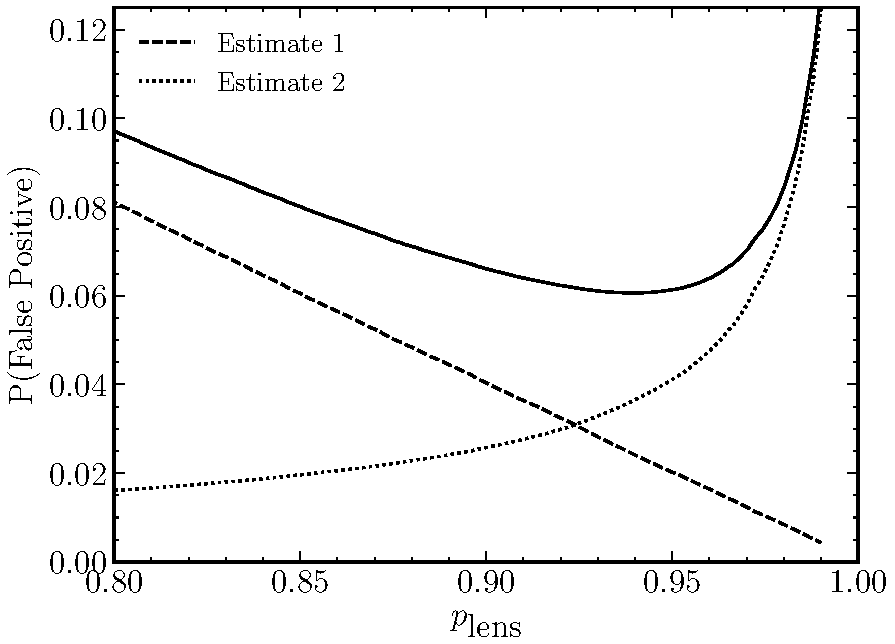
\includegraphics[width=0.62\columnwidth]{Figures/Figure_2_11.pdf}
    \caption[Fraction of unlensed sources in our lensed sample as a function of $p_\textrm{lens}$]{The false positive rate, the fraction of sources in the lensed catalogue that are unlensed, as a function of the threshold probability for gravitational lensing, $p_\textrm{lens}$. The false positive rate is split into two components: the first calculated assuming that the probability of any source, $i$, not being lensed is given by $1 - p_{\textrm{lens, i}}$ (dashed line), the second estimated from the fraction of sources in the reliable ($R > 0.8$) SGP sample that are likely to be spuriously matched to a VIKING counterpart and have a far-IR predicted redshift large enough that the \textit{Herschel} galaxy is more likely contained in the lensed catalogue than not (dotted line). The total is the combination of the two estimates (solid line).}
    \label{fig:lens_false_positive}
\end{figure}

A notable disadvantage of this method is that it relies on having matched a \textit{Herschel} source to a near-IR counterpart with high reliability. In reality, these high probability matches are the locations of galaxies where we are most confident that the near-IR galaxy is the source of the dust emission. This leads to an underestimate of the true number of lensing events. We could lower the reliability threshold for this calculation, but the false identifications rates become much more uncertain.

We also applied this method to the subset of sources with $S_{500} > 100\,$mJy. From the $41$ candidates listed in Appendix \ref{app:candidate_lenses_bright}, $24$ have near-IR counterparts with $R > 0.8$ and $19$ of these have a photometric redshift from the HELP catalogue. In most cases the probability of gravitational lensing is greater than $0.95$ and the mean probability is $0.89$. This suggests two things, one, that the bright candidates are indeed likely to be sources lensed by a VIKING foreground object, and two, that the simple method described above may be a reasonably accurate measure of lensing events in \textit{Herschel} fields for lower flux densities.

\subsection{Number Counts and Redshift Distribution of Lensed Candidates}
\label{sec:lensed_number_counts}

To assess how well our simple selection method compares to galaxy evolution models, we compare the redshift distribution and number counts of \textit{potentially} lensed \textit{Herschel} sources with the predictions from the evolution model of \citealt{Cai_2013}. When comparing the source counts from the $\sim 16\,$deg$^2$ SDP field to a selection of models, it was found that the model of \citealt{Negrello_2007} gave the closest match to observations (\citealt{Clements_2010}). Given that the work of \citealt{Cai_2013} is a development of the \citealt{Negrello_2007} model, and it also incorporates the effect of strong gravitational lensing, it should be suitable for comparison with the observations in the SGP. The galaxy evolution model of \citealt{Cai_2013} combines a physical, forward model for protospheroidal galaxies and AGN at $z \geq 1.5$ with a phenomenological backward model for late-type galaxies at $z \leq 1.5$. At these lower redshifts, the model assumes a combination of `warm' starburst galaxies and `cold' normal-type galaxies. The model also incorporates the effect of gravitational lensing on the observed source counts of these galaxies at IR wavelengths, assuming a fixed magnification value. To compare with the lensed candidates described here, we chose to use a variant of the \citealt{Cai_2013} model where the maximum magnification due to gravitational lensing is set at $\mu = 12$, a value that provides good agreement with the lensed number counts of \citealt{Negrello_2017}.

We combined together the sources with $p_{\textrm{lens}} > 0.94$ with the bright candidates from Section \ref{sec:brightest_lenses} to create a complete sample of SGP lensing candidates. In the top panel of Figure \ref{fig:lens_distributions_against_cai} we show the redshift distribution for all SGP sources (solid black line) as well as the redshift distribution of lensed sources (solid red line) and their deflectors (solid pink line). We compare these to the predictions from \citealt{Cai_2013}, which are shown using dashed lines of the same colours. The distributions show that while the total number of sources is well predicted by the model, there is a large discrepancy in the number of lensed systems at all redshifts. When illustrated as a function of the $500\,\mu$m flux density (middle panel), we see that the large disagreement in the counts of lensed sources comes from low flux densities. This discrepancy is corroborated by the lensing fraction -- the fraction of all galaxies that are likely being lensed -- shown in the bottom panel of Figure \ref{fig:lens_distributions_against_cai}. While the model of \citealt{Cai_2013} predicts that the probability of lensing is very low and approaching zero at low flux densities, the candidate lenses in the SGP continue to contribute $\sim 5 - 10\%$ of the total source counts at close to the detection limit at $500\,\mu$m.

A possible explanation for the underprediction of the number of lenses in the SGP by the \citealt{Cai_2013} model is that it is limited to strong lensing ($\mu > 2$) events, whereas our simple method relies solely on the redshifts of the galaxies and thus is not limited by their apparent brightness. Studies of the spatial cross-correlation between \textit{Herschel} galaxies in the GAMA fields and SDSS galaxies (\citealt{Gonzalez-Nuevo_2014, Gonzalez-Nuevo_2017}) have shown that the amplification of clustered galaxies by foreground structures can be explained by weak gravitational lensing ($\mu < 2$). These studies have shown that the majority of magnification bias occurs not from single galaxies, but from small groups of galaxies with one or two massive galaxies and several satellites. We may therefore ask ourselves whether our discrepancy with the \citealt{Cai_2013} model is due to the inclusion of strong and weak gravitational events, and that VIKING galaxies may act as signposts to the locations of galaxy groups.

\begin{figure}
    \centering
    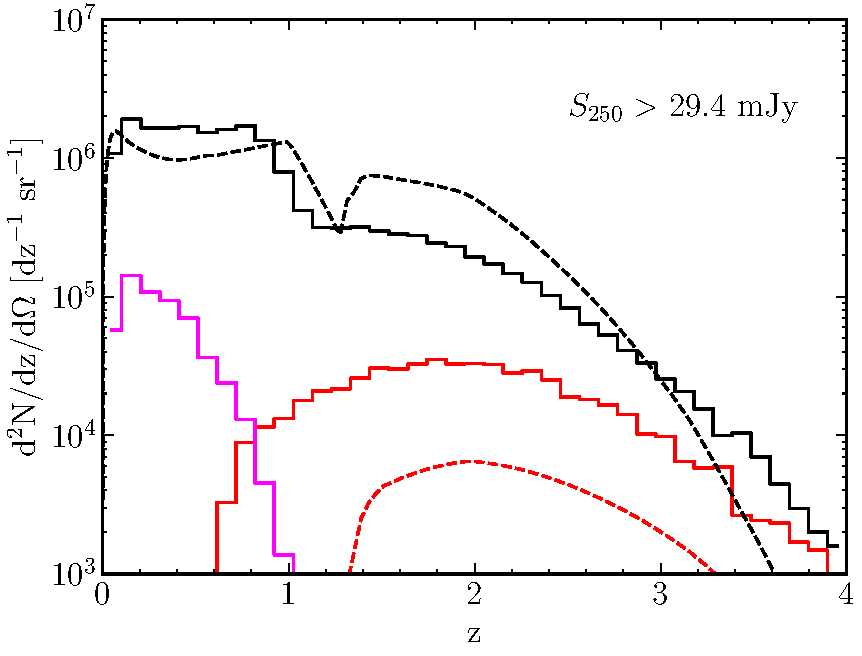
\includegraphics[width=0.55\columnwidth,height=0.255\textheight]{Figures/lens_redshift_distribution.pdf}
    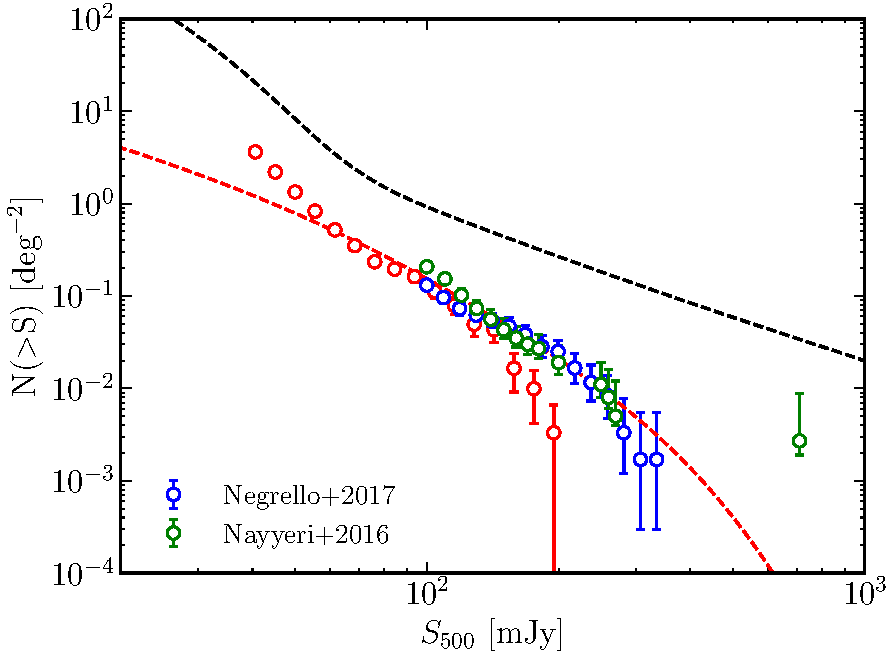
\includegraphics[width=0.55\columnwidth,height=0.255\textheight]{Figures/lens_number_counts.pdf}
    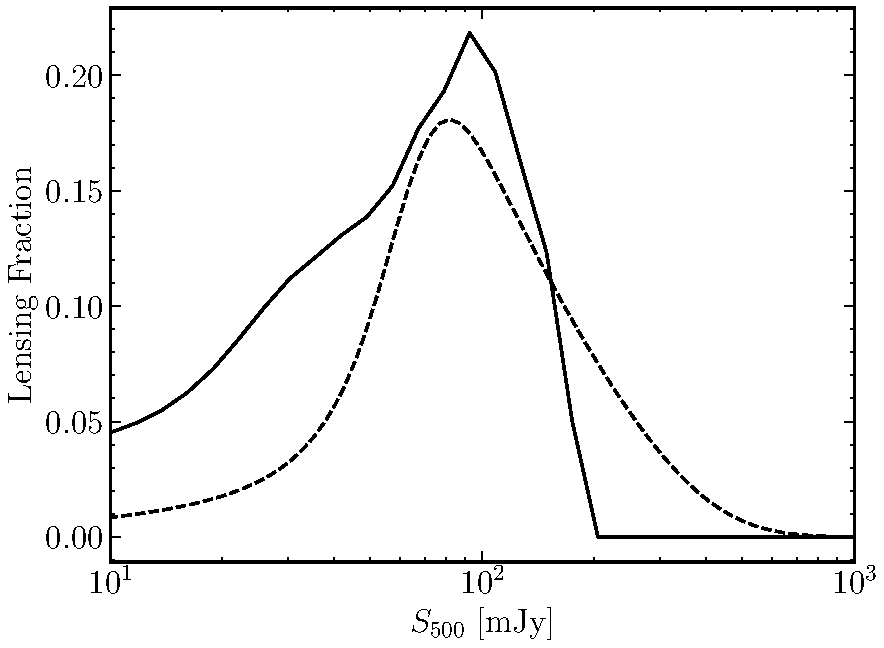
\includegraphics[width=0.55\columnwidth,height=0.255\textheight]{Figures/lensing_fraction.pdf}
    \caption[Comparison of our unlensed and lensed galaxy populations]{Top panel: The photometric redshift distribution of \textit{Herschel} sources (solid black line), as well as the distribution of lensed sources (solid red line) and their deflectors (solid pink line). The predictions from the \citealt{Cai_2013} model are shown as dashed lines using the same colours, except for the distribution of foreground deflectors which are not provided as part of the model. Middle panel: The cumulative number counts as a function of $500\,\mu$m flux density, using the same colour convention as above. The observations are now shown as error bars alongside the studies of \citealt{Nayyeri_2016} (green error bars) and \citealt{Negrello_2017} (blue error bars). Bottom panel: The fraction of sources that we predict are lensed in the SGP as a function of $500\,\mu$m flux density (solid black line), compared to the prediction from \citealt{Cai_2013} (dashed black line).
    \label{fig:lens_distributions_against_cai}}
\end{figure}

\section{Conclusions}

In this Chapter, we introduced the \textit{Herschel}-ATLAS project and implemented the Likelihood Ratio method for identifying near-IR counterparts to \textit{Herschel} sources in the South Galactic Pole field. We predicted the efficacy of the method by estimating the completeness, cleanness, and false identification rate of our sample. For $193,527$ \textit{Herschel} sources in the field, we were able to reliably match $110,374$ ($57\%$) with a VISTA VIKING counterpart, to greater than $80\%$ confidence. The completeness of the sample is $78\%$ and the false identification rate is expected to be approximately $5\%$. The data products for the H-ATLAS project are now complete\footnote{The H-ATLAS project can be found at https://www.h-atlas.org.}. In total, the survey detected over $400,000$ sources at $250\,\mu$m over $660\,$deg$^2$, with approximately half of these being matched with high significance to an optical or near-IR object. As a result, the $100,000$ newly identified far-IR bright galaxies presented here represent a doubling in the size of the H-ATLAS catalogue with reliable IDs. We showed from the similarity in the photometric redshifts of counterparts that there are likely to be between $400$ and $1,000$ sources in the SGP field that are the result of multiple VIKING galaxies. Finally, we searched for gravitational lensing events and observed $41$ bright candidates (with $500\,\mu$m flux densities greater than $100\,$mJy) and presented a method that predicts a further $\sim 6,000$ strong and weak lensing events that could be observed at lower flux densities. In the following Chapter, we shall estimate some fundamental properties of the interstellar dust in these galaxies, and from them, estimate the dust content in galaxies over cosmic time.


\chapter{Redshift Evolution of the Dust Mass Function}
\label{chapter:Dust_Mass_Functions}
\sloppy

\section{Introduction}

As discussed in Chapter \ref{chapter:Introduction}, dust is composed of metals that are produced from stellar nucleosynthesis, and then expelled into the ISM via supernovae and stellar winds. While some fraction of these metals mix with the gas phase in the ISM, around $30 - 50\%$ of the metals condense into dust grains (\citealt{Draine_2007b}). If this fraction of metals that get locked up in dust grains is somewhat consistent over time, then dust may be considered a useful tracer of gas metallicity in a galaxy. For this reason, the total mass of dust in the ISM can be used to study the evolutionary stage of the galaxy (e.g. \citealt{Cortese_2012, deVis_2017a, deVis_2017b}). Moreover, dust is not just the product of previous star formation, but also, as the site of molecule formation like $H_2$, it has a significant influence on the formation of molecular clouds for future star formation. Understanding the dust content of galaxies over cosmic time is therefore important in providing insight into the evolution of galaxies and their ISM. In this Chapter, we estimate the dust masses of the galaxies in the South Galactic Pole field and derive the far-IR selected dust mass function (DMF), the space density of galaxies as a function of dust mass, in redshift slices of width $0.2$ out to $z = 1$.

\section{Local and High Redshift DMFs in the Literature}

The first direct measurements of the far-IR/sub-mm derived DMF were with SCUBA using the SCUBA Local Universe Galaxy Survey \mbox{(SLUGS: \citealt{Dunne_2000, Dunne_2001, Vlahakis_2005})}, a survey of local \textit{IRAS}-selected galaxies. However, these studies were limited by small number statistics and were typically limited to very small redshifts. A high redshift ($z = 2.5$) DMF for comparison was presented in \citealt{Dunne_2003}, suggesting that galaxies with the highest dust masses have an order of magnitude more dust than locally (assuming pure dust mass evolution and no evolution in the number density of the most massive galaxies). Improvements were made with the introduction of BLAST, which allowed for the derivation of the DMF from a sample of galaxies selected at wavelengths spanning the peak of the far-IR spectrum (the same wavelengths as the \textit{Herschel}-SPIRE instrument). \citealt{Eales_2009} used BLAST data to arrive at similar conclusions, that there is strong evolution in both the $250\,\mu$m luminosity function (LF) and in the DMF out to $z = 1$. The concurrence of the two suggesting that the evolution in the far-IR/sub-mm luminosity of these galaxies is directly related to the increase in the size of their dust reservoirs. However, this study was also limited by small number statistics ($\sim 100$ sources).

The first study to measure the evolution in the DMF using the large area of H-ATLAS was \citealt{Dunne_2011}, using a $250\,\mu$m selected sample of $1,867$ sources from the Science Demonstration Phase (SDP). This represented a sample an order of magnitude larger than previous studies, allowing for a significant direct measurement of the space-density of galaxies as a function of dust mass, out to a redshift of $0.5$. As we explored in the previous Chapter, the upper redshift limit of this study was set by the limiting magnitude of the optical surveys in the \textit{Herschel} fields. The main finding from this study was that the integrated dust density of the Universe, that is the total dust mass in a given cosmological volume, evolves with redshift according to $\rho_{\textrm{dust}} \propto (1+z)^{4.5}$ between $0 < z < 0.5$. The local density was estimated to be $\rho_{\textrm{dust}, (z=0)} = 9.8\times10^4$\,$M_\odot$Mpc$^{-3}$. This work was further developed in \citealt{Beeston_2018} where the authors derived the local ($z < 0.1$) DMF from $\sim 16,000$ galaxies, the largest H-ATLAS sample at the time of the study, using the aforementioned crossmatching between the H-ATLAS and the GAMA spectroscopic survey detailed in \citealt{Bourne_2016}. The sample size of \citealt{Beeston_2018} permitted significant numbers of galaxies with dust masses as low as $\sim 10^4\,M_\odot$ and therefore extended the observed mass range by at least an order of magnitude compared to previous measurements. This gave better constraints on the low mass end of the DMF which, despite accounting for a negligible amount of the dust budget compared to the most massive galaxies, contribute substantially in number. This low mass regime is constrained by sources that tend to be nearby and faint, and suffer from low numbers in flux-limited surveys such as H-ATLAS, thus this study provides important measurements in an otherwise uncertain region of the DMF. The large sample size of the \citealt{Beeston_2018} study means that the measurement of the low mass end of the DMF from this work is currently our best estimate. Despite differences in the measured number density of low mass galaxies, \citealt{Dunne_2011} and \citealt{Beeston_2018} both have local dust mass densities (DMD) in good agreement. More recently, \citealt{Driver_2018} produced an extended DMF and measured the DMD out to $z = 5$. This study was based on an optically-selected sample of approximately $570,000$ galaxies from GAMA, G10-COSMOS (\citealt{Davies_2015}; \citealt{Andrews_2017}) and 3D-HST (\citealt{Brammer_2012, Momcheva_2016}). Unlike \citealt{Dunne_2011}, this study found no evidence for a strong evolution in the dust content of galaxies in the past $5\,$Gyr, instead observing a flat DMD since $z = 0.5$. However, an apparent evolution is observed in the dust luminosity which would suggest that a strong evolution in dust temperature is required in order to maintain a flat DMD. Other notable works that measure the evolution of the DMF to high redshifts include \citealt{Pozzi_2020} and \citealt{Dudzeviciute_2021}. The former derived the DMF from $z \sim 0.2$ to $z \sim 2.5$ using a $160\,\mu$m \textit{Herschel}-PACS selected catalogue of approximately $5,300$ galaxies in the COSMOS field. In accordance with \citealt{Driver_2018}, they find a peak in the redshift evolution of the DMD at $z \sim 1$, but more in keeping with \citealt{Dunne_2011}, they also observe a decreasing trend from the peak in dust density to the present day. The implication of such varied results is that consistency among studies depends largely on the selection wavelength of the sample, the survey area and any assumptions that may be made during the measurement of the dust masses of the galaxies. We note that of the studies mentioned here, the sample of \citealt{Pozzi_2020} is selected from the shortest wavelength ($160\,\mu$m), which may explain some of the differences observed between this study and the other, \textit{Herschel}-selected samples. This will be explored further in Section \ref{sec:schechter_functions}. Finally, \citealt{Dudzeviciute_2021} add valuable constraints on the DMF at $z = 1 - 2$ and $z = 3 - 4$ based on two samples selected at wavelengths corresponding to nearly identical rest frame $\sim 180\,\mu$m populations. Between $1 < z < 2$, \citealt{Dudzeviciute_2021} studied the dust properties of $121$ SMGs from the $450\,\mu$m SCUBA-2 Ultra Deep Imaging EAO Survey (STUDIES: \citealt{Wang_2017, Chang_2018, Lim_2020b, Lim_2020c}) and compared these results to an $850\,\mu$m SMG sample with redshifts between $3 < z < 4$ from the ALMA/SCUBA-2 Ultra Deep Survey (AS2UDS: \citealt{Stach_2018, Stach_2019, Dudzeviciute_2020}). 

In this study, we derive the DMF from the galaxies observed in the H-ATLAS SGP field presented in Chapter \ref{chapter:Data_Release_3}. We include in our study those galaxies matched with high reliability ($R > 0.8$) to a VIKING counterpart with an estimated redshift from the HELP catalogue. The dust masses are calculated from the \textit{Herschel}-SPIRE $250\,\mu$m flux densities, and thus our estimates of the DMF are likely to follow similar observed trends as in the previous H-ATLAS studies of \citealt{Dunne_2011} and \citealt{Beeston_2018}. The work presented here allows us to expand on these works by extending the \textit{Herschel} predicted DMF to higher redshifts as a result of the increased depth from the near-IR crossmatching. In addition, we implement an error analysis that propagates errors in the photometric redshifts through to the final DMF, allowing us to use a sample devoid of spectroscopic redshifts. The spectroscopic coverage of the SGP is much lower than for the GAMA fields, but by propagating the photometric redshift errors through our analysis, we can define a signifcantly sized sample of galaxies, providing they fulfill three criteria: i) they are classified as galaxies (Section \ref{sec:star_galaxy_classifier}), ii) they have a near-IR counterpart that has been matched with a high probability, and iii) have an associated redshift. We shall use the photometric redshifts from the \textit{Herschel} Extragalactic Legacy Project (HELP, Section \ref{sec:phot_z_VIKING}). This corresponds to a sample of $81,895$ galaxies, making it the largest sample of \textit{Herschel} galaxies used to study the dust content of the Universe.

\section{Dust Properties of H-ATLAS Galaxies}

To measure the dust masses of our SGP galaxies, we require observations from the same rest frame wavelengths, regardless of their redshift. With select \textit{Herschel} wavebands to work with, we must be able to K-correct their dust spectra to a given rest frame wavelength. This in turn requires us to have an understanding of what a typical dust SED might look like at all far-IR wavelengths. Although galaxies contain dust with a range of temperatures, previous studies have shown that most interstellar dust grains have a cold temperature of $\sim 20\,$K (e.g. \citealt{Dunne_2001, Vlahakis_2005, Draine_2007a, Boselli_2010, Smith_2012b, Smith_2013}). Dust close to sources of heating such as star forming regions and AGN have higher temperatures and radiate at rest frame wavelengths $\lesssim 100\,\mu$m. These grains can influence the temperature measured from an isothermal dust model. To account for this mixing of dust temperatures, the ideal scenario would be to estimate the dust mass of a galaxy using a mass-weighted temperature of the dust. This would require fitting a model with multiple different dust temperatures and weighting the temperatures by the mass of the dust for that component. We observed such an example earlier when we described the H-ATLAS galaxies using the two-temperature model of \citealt{Pearson_2013}. However, it has already been shown that the cold dust reservoir at $\sim 20\,$K has the most signifcant contribution by mass (\citealt{Pearson_2013}) and the difference between the mass weighted dust temperature and the isothermal temperature is often not significant (e.g. \citealt{Clark_2015}). For example, if we assume that H-ATLAS galaxies are well approximated by the two temperature model of \citealt{Pearson_2013} (where $T_{\textrm{hot}} = 46.9\,$K, $T_{\textrm{cold}} = 23.9\,$K and $\alpha = M_c/M_h = 30.1$), then the mass weighted temperature is given by $T_{\textrm{dust, weighted}} = (M_cT_c + M_hT_h)/(M_c + M_h) \approx 24.6\,$K, which is only marginally warmer than the cold dust component. Hot dust has the greatest effect on the SED at wavelengths less than the peak wavelength ($\sim 100\,\mu$m in the rest frame). For galaxies at $z < 1$, the \textit{Herschel} flux measurements are at wavelengths larger than the peak wavelength, and thus the best fitting value, which reflects a luminosity weighted temperature, is expected to be similar to the temperature of the cold dust component in a two-component model. By extension, the isothermal dust temperature from the SED fitting of \textit{Herschel} flux densities alone should be a reasonable approximation to the mass weighted dust temperature.

In addition, to include hot dust at $\lambda_{\textrm{rest}} \lesssim 100\,\mu$m, we would require short wavelength photometry (presumably from PACS) with significant SNR to be able to put meaningful constrains on a second temperature component. As shown in Table \ref{tab:snr_fraction}, the percentage of galaxies in our sample that have significant detections at the PACS wavelengths decreases rapidly with redshift to as low as $\sim 6 - 8\%$ by just $z \sim 0.3$. With so few galaxies in our redshift range having PACS detections with useful SNR, the ability to adequately fit an SED to the \textit{Herschel} observations is essentially the same whether we are considering an isothermal or multi-component model. The benefit of assuming an isothermal model in this instance is the reduction in the number of model parameters.

\begin{table}
    \centering
    \begin{tabular}{p{3cm}|p{1.75cm}|p{1.75cm}|p{1.75cm}|p{1.75cm}|p{1.75cm}}
        \hline
        \hline
        Redshift Interval & 100\,\micron & 160\,\micron & 250\,\micron & 350\,\micron & 500\,\micron \\
         & [> 3$\sigma$] & [> 3$\sigma$] & [> 4$\sigma$] & [> 4$\sigma$] & [> 4$\sigma$] \\
        \hline
        \hline
        0 < z < 0.2 & 22.6 & 28.0 & 99.3 & 31.4 & 5.0 \\
        0.2 < z < 0.4 & 6.0 & 7.8 & 98.6 & 20.3 & 2.7 \\
        0.4 < z < 0.6 & 3.0 & 4.4 & 96.9 & 28.1 & 4.6 \\
        0.6 < z < 0.8 & 1.4 & 2.8 & 96.0 & 37.5 & 6.7 \\
        0.8 < z < 1 & 0.9 & 2.1 & 95.3 & 45.0 & 8.0 \\
        \hline
    \end{tabular}
    \caption[The significance of \textit{Herschel} observations in redshift slices to $z = 1$]{The percentage of sources in our galaxy sample that have detections in each \textit{Herschel}-PACS and \textit{Herschel}-SPIRE waveband at the level of significance indicated in the column headers. The percentages are shown for redshift bins of width $0.2$, the same used for deriving the binned dust mass functions.}
    \label{tab:snr_fraction}
\end{table}

Without sufficient data to constrain the dust temperature and $\beta$ simultaneously, we assume a fixed $\beta = 2$ and fit an isothermal modified blackbody to all galaxies. In Figure \ref{fig:dust_temperatures} we plot the distribution of measured dust temperatures as a function of photometric redshift. We see that the median value at all redshifts is consistent with $20\,$K, which we shall assume herein as the typical temperature of the cold ISM. The righthand panel of Figure \ref{fig:dust_temperatures} shows the distribution of dust temperatures (black histogram) and the contributions from galaxies with one (red), two (blue) and three (green) SPIRE observations with flux densities at greater than $4\sigma$ significance. As previously shown by \citealt{Beeston_2018} the galaxies with significant \textit{Herschel} fluxes in all three SPIRE wavebands are on average colder than those with only one or two bands. This illustrates a simple selection effect of the \textit{Herschel} observations. If a galaxy is detected at $250\,\mu$m, then it is more likely to also have detections at longer wavelengths if the dust is colder than average (the far-IR SED shifts to longer wavelengths at colder dust temperatures).

\begin{figure}
	\centering
	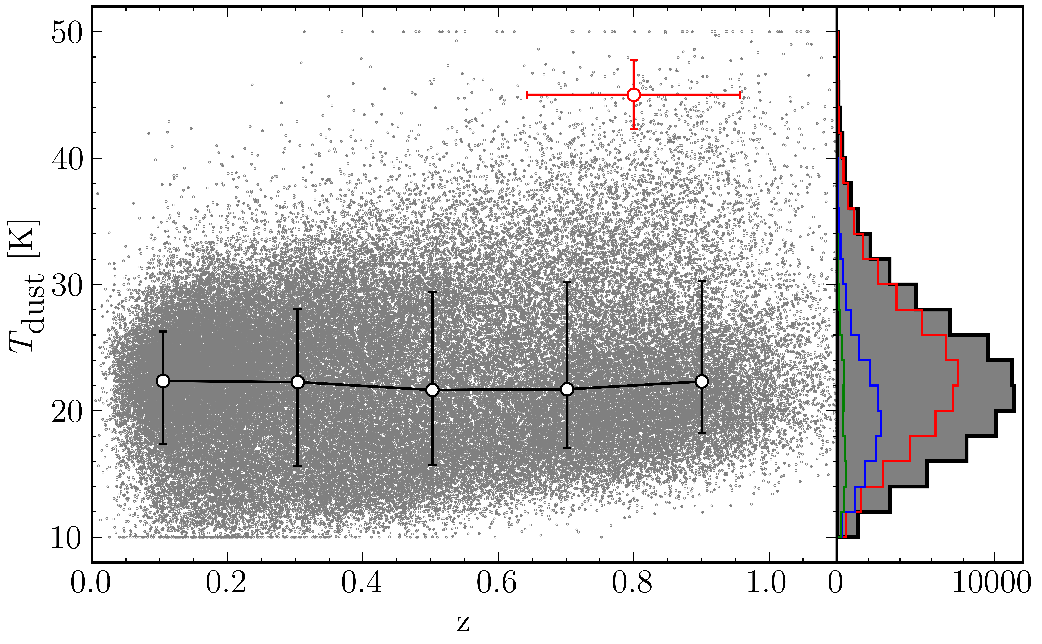
\includegraphics[width=0.8\columnwidth]{Figures/dust_temperatures.pdf}
	\caption[The distribution of dust temperatures as a function of redshift]{The dust temperature against redshift for galaxies in the SGP field. The red cross illustrates the typical $1\sigma$ error in the redshifts and dust temperatures. The black error bars represent the median dust temperature in each redshift bin, along with the $1\sigma$ range in the distribution ($16$th to $84$th percentiles). The righthand panel shows the histogram of dust temperatures for all galaxies (grey filled), galaxies with SNR $> 4$ in one band (red), in two bands (blue) and in three bands (green).}
	\label{fig:dust_temperatures}
\end{figure}

In the next section we shall start from the assumption that the dust spectrum of all galaxies in our sample can be approximated by an SED with a characteristic dust temperature of $20\,$K when deriving the DMF (e.g. \citealt{Vlahakis_2005}). This knowledge is required for certain methods used to derive a binned DMF in $M_{\textrm{dust}}-z$ space as they rely on knowing the shape of the SED to apply appropriate K-corrections in each bin. As we shall explain later, some methods for calculating binned functions allow for each galaxy to use its own dust spectrum rather than a global SED to compute the required K-corrections. We shall discuss how this impacts our DMF in later sections.

We calculate dust masses from monochromatic rest frame luminosities, which we derive from the K-corrected observed flux densities at $250\,\mu$m. We translate the $250\,\mu$m flux densities of the SGP galaxies into monochromatic luminosities using

\begin{equation}
    L_{250} = \frac{4\pi D_L^2 S_{250}K}{(1+z)},
\label{eq:monohromatic_luminosities}
\end{equation}

\noindent where $L_{250}$ is in units of W Hz$^{-1}$, $D_L$ is the luminosity distance, $S_{250}$ is the observed flux density at $250\,\mu$m and $K$ is the K-correction that allows us to define a rest frame quantity at $250\,\mu$m in terms of the observed frame at the same wavelength, given by

\begin{equation}
    K = \frac{S_{250}^{K}}{S_{250}^{\textrm{obs}}} = \Bigg(\frac{\nu_{K}}{\nu_{\textrm{obs}}}\Bigg)^{3+\beta}\frac{e^{(h\nu_{\textrm{obs}}/kT)} - 1}{e^{(h\nu_{K}/kT)} - 1},
\label{eq:k_correction}
\end{equation}

\noindent where $\nu_{K} = \nu_{\textrm{obs}}(1+z)$ and $T$ and $\beta$ are the dust temperature and emissivity index describing the SED. 

Let us briefly consider a galaxy at the edge of our redshift range, $z \sim 1$. The factor $K$ allows us to convert $S_{250}^{\textrm{obs}}$, the emission radiated at $250\,\mu$m ($1.2\,$THz) and observed at $125\,\mu$m ($2.4\,$THz) to $S_{250}^{K}$, the $250\,\mu$m flux density in the galaxy's rest frame. The monochromatic luminosity at $250\,\mu$m is then converted to a dust mass using

\begin{equation}
    M_{\textrm{dust}} = \frac{L_{250}}{4\pi\kappa_{250}B(\nu_{250}, T)},
\label{fig:dust_mass}
\end{equation}

\noindent where $\kappa_{250}$ is the dust mass absorption coefficient at $250\,\mu$m. The dust mass absorption coefficient is an amalgamation of terms including the efficiency with which the dust grains emit in reference to a perfect blackbody, the size of the dust grains and their mass volume density. For this reason, the value of $\kappa_\nu$ is highly uncertain with a wide range of values spanning multiple orders of magnitude being presented in the literature (\citealt{Clark_2019}). A commonly used value is $0.077\,$m$^2$kg$^{-1}$ at $850\,\mu$m (\citealt{Dunne_2000, daCunha_2008, Dunne_2011}) which represents a theoretical value lying between the expected value for graphite and silicate dust grains (\citealt{Draine_1984}). Assuming $\beta = 2$ we scale this value to $250\,\mu$m such that $\kappa_{250} = 0.89\,$m$^2$kg$^{-1}$.

\section{Sources of Incompleteness}

An important issue to consider when deriving our DMF is the completeness of our \textit{Herschel} survey and how we may account for missing galaxies when estimating the space-density of objects. In the following sections we outline the methods we use to estimate the incompleteness of our sample and thus the completeness correction factors we apply to our SGP catalogue, in order to account for sources we either do not observe or do not retain from the LR method described earlier. Each object in our SGP sample will be multiplied by correction factors that compensate for the number of times we might expect to observe this type of galaxy, based on the number of missing \textit{Herschel} sources and sources without a near-IR identification.

\subsection{\textit{Herschel} Catalogue Incompleteness}

The first correction factor is a direct result of the source extraction process used to create the \textit{Herschel} catalogues from the far-IR images. Due to source confusion these catalogues are incomplete as we approach the flux limit of the survey. To determine the completeness of the H-ATLAS catalogues, \citealt{Valiante_2016} used a catalogue of simulated sources embedded in real H-ATLAS maps to predict the efficiency of the \texttt{MADX} algorithm in recovering the sources. The completeness is shown as a function of the measured $250\,\mu$m flux density in Figure \ref{fig:submm_completeness} and is listed in Table \ref{tab:submm_completeness_table} along with the correction factors, $c_{\textrm{far-IR}}$, defined as the reciprocal of the completeness. We use an interpolated version of this table when applying the correction factors to our SGP galaxies. Unsurprisingly, the highest correction factors are found as we approach the flux limits of the survey where confusion noise dominates and the likelihood of lost sources rises.

\begin{table}
    \centering
    \begin{tabular}{p{5cm}|p{2.5cm}|p{2.5cm}}
        \hline
        \hline
        $250\,\mu$m Flux Density [mJy] & Completeness & $c_{\textrm{far-IR}}$ \\
        \hline
        \hline
        20.0 & 0.541 & 1.849 \\
        26.5 & 0.762 & 1.313 \\
        35.1 & 0.903 & 1.107 \\
        46.4 & 0.969 & 1.032 \\
        61.5 & 0.989 & 1.011 \\
        81.4 & 0.993 & 1.007 \\
        107.7 & 0.997 & 1.003 \\
        142.6 & 0.997 & 1.003 \\
        188.8 & 0.997 & 1.003 \\
        250.0 & 0.999 & 1.001 \\
        \hline
    \end{tabular}
    \caption[Far-IR catalogue completeness as a function of $250\,\mu$m flux density]{The far-IR completeness and corresponding correction factors as a function of the measured flux density.}
    \label{tab:submm_completeness_table}
\end{table}

\subsection{Reliable ID Incompleteness}

The second correction function arises from our inability to match all the \textit{Herschel} sources, for which we have observed a candidate on the VIKING image, with a high reliability counterpart. The unmatched sources are largely the result of large positional uncertainties, the possibility of coincident background objects and multiple systems where the sources are associated with each other but treated independently by the LR method.

In its simplest form, the completeness of our reliable sample is defined as the redshift distribution of our IDs divided by the true redshift distribution of \textit{Herschel} counterparts, scaled to the number of sources for which we observe a nearby VIKING counterpart; $C_{\textrm{id}} = n_{\textrm{reliable}}(z)/n_{\textrm{real, scaled}}(z)$. This second term is closely related to the probability distribution of true counterparts as a function of redshift, $q(z)$, much like the true counterparts distribution we derived as a function of $K_s$-band magnitude in the previous Chapter. Using the same formalism as Equation \ref{eq:true_counterparts_distribution}, we define the denominator as

\begin{equation}
    n_{\textrm{real, scaled}} = q(z)\times N_{\textrm{250\,\micron}} = \frac{n_{\textrm{real}}(z)}{\sum_{z_i}n_{\textrm{real}}(z_i)}\times QN_{\textrm{250\,\micron}},
    \label{eq:n_real_scaled}
\end{equation}

\noindent where $n_{\textrm{real}}(z)$ is the redshift distribution of true counterparts (recall Equation \ref{eq:real_distribution}) and $N_{\textrm{250\,\micron}}$ is the number of $250\,\mu$m \textit{Herschel} positions. As previously, the required correction functions are the reciprocal of the completeness. When we derived the $q(m)$ distribution in Section \ref{sec:true_counterparts_distribution} we noted that the distribution is normalized such that the integral of $q(m)$ up to the limiting magnitude of the VIKING survey is equal to the probability that the source is detected ($\int^{m_\textrm{lim}} q(m) dm = Q$). As an extension of this normalization, we recognize that the integral of the ID redshift distribution multiplied by the correction factors should give the total number of sources with observable counterparts (i.e. $\int_z c_{\textrm{id}} n_{\textrm{reliable}}(z) dz = QN_{\textrm{250\,\micron}}$, where $c_{\textrm{id}}$ are the correction factors given by $1/C_{\textrm{id}}$).

The ID completeness as a function of redshift is listed in Table \ref{tab:id_completeness_table} and illustrated in Figure \ref{fig:id_completeness} alongside the completeness functions from the SDP (\citealt{Smith_2011}), GAMA9 field (\citealt{Fleuren_2012}) and NGP (\citealt{Bourne_2016}). The average correction factor per source in the SGP is approximately two. Near the median redshift of the distribution ($z \sim 0.5$) the completeness is lower in the SGP than in other fields, though we note that we do not include spectroscopic redshifts, which might lower our completeness. The general trend for all H-ATLAS studies is a steady decline from $\sim 100\%$ completeness at $z = 0$ to a minimum at $z \sim 0.5 - 0.7$ followed by a rise at higher redshifts. The decrease towards $z = 0.5$ might be a result of a fixed search radius corresponding to a greater physical scale at larger cosmological distances. This would result in a greater probability of observing spurious counterparts that decrease the ID rate. Presently, we are not sure why the ID completeness rises again at higher redshifts, but one possible explanation is the greater probability of lensing events along the line of sight 

\begin{table}
    \centering
    \begin{tabular}{p{4.5cm}|p{2.5cm}|p{2.5cm}}
        \hline
        \hline
        Redshift & Completeness & $c_{\textrm{id}}$ \\
        \hline
        \hline
        0.05 & 0.984 & 1.016 \\
        0.15 & 0.881 & 1.135 \\
        0.25 & 0.713 & 1.403 \\
        0.35 & 0.542 & 1.844 \\
        0.45 & 0.432 & 2.313 \\
        0.55 & 0.387 & 2.581 \\
        0.65 & 0.372 & 2.685 \\
        0.75 & 0.360 & 2.776 \\
        0.85 & 0.392 & 2.552 \\
        0.95 & 0.422 & 2.369 \\
        \hline
    \end{tabular}
    \caption[ID completeness as a function of redshift]{The counterpart ID completeness and corresponding correction factors as a function of redshift.}
    \label{tab:id_completeness_table}
\end{table}

\begin{figure}
	\centering
	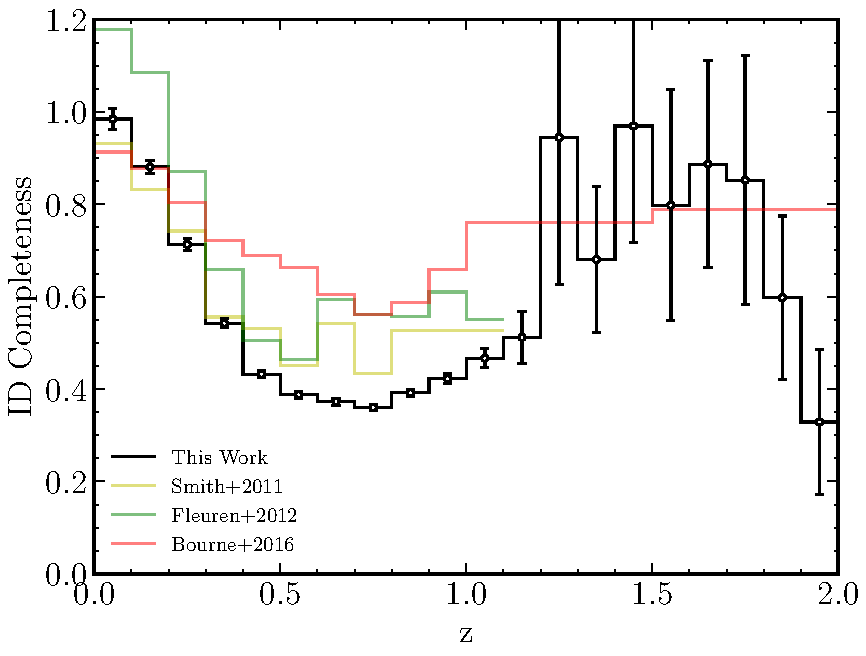
\includegraphics[width=0.8\columnwidth]{Figures/id_completeness.pdf}
	\caption[Completeness of our reliable SGP sample as a function of redshift]{The completeness of our $R > 0.8$ SGP sample as a function of redshift (black error bars), calculated using $n_{\textrm{reliable}}(z)/n_{\textrm{real, scaled}}$ where $n_{\textrm{real, scaled}}(z)$ is given by Equation \ref{eq:n_real_scaled}. Completeness functions from other H-ATLAS studies; \citealt{Smith_2011}, \citealt{Fleuren_2012} and \citealt{Bourne_2016}, are shown as yellow, green and red lines, respectively.}
	\label{fig:id_completeness}
\end{figure}

\section{Estimators of the Binned Dust Mass Function}
\label{sec:dmf_estimators}

The dust mass function, $\phi(M_{\textrm{dust}})$, represents the space density of galaxies as a function of dust mass, which in its differential form is given as the number of galaxies per unit comoving volume per unit dust mass interval

\begin{equation}
    \phi(M_{\textrm{dust}}, z) = \frac{d^2N}{dV dM_{\textrm{dust}}},
\label{eq:differential_phi}
\end{equation}

\noindent where $N$ is the number of galaxies with dust mass $M_{\textrm{dust}}$ observed in the comoving volume $V$ at redshift $z$. In this section we outline two methods of calculating the binned dust mass function; the ubiquitously used $1/V_{\textrm{max}}$ method \mbox{(\citealt{Schmidt_1968, Felten_1976, Avni_1980})} and the approximate method, $\phi_{\textrm{est}}$, proposed by \citealt{Page_2000}. Alternative parametric methods (e.g. the maximum-likelihood method of \citealt{Marshall_1983}) allow us to explore the entire $M_{\textrm{dust}} - z$ space, including regions that are not covered by observational data, and allow us to produce continuous functions for $\phi(M_{\textrm{dust}}, z)$. Although it is well established that the dust mass function can be parameterized in the form of a Schechter function (\citealt{Press_1974, Schechter_1976}), it is not obvious how this function evolves with redshift and which functional form should be used for this evolution. For this reason, we prefer to use binned, non-parametric methods and empirically study the redshift evolution of the DMF.

\subsection{The $1/V_{\textrm{max}}$ Method}

The prevalent use of the $1/V_{\textrm{max}}$ method stems from our need to overcome the Malmquist bias (\citealt{Eddington_1914, Malmquist_1922}) that causes selection biases in flux density limited samples. Malmquist bias refers to the tendency for flux-limited samples to be increasingly dominated by more luminous sources with increasing cosmological distance. As a result, more luminous objects are detected in larger volumes than less luminous objects, which needs to be accounted for in our space-density calculations. The $1/V_{\textrm{max}}$ method corrects for this bias by weighting each galaxy according to the maximum comoving volume in which it can be observed by the survey. The number density of galaxies in a given dust mass-redshift bin ($\Delta M_{\textrm{dust}} \Delta z$) is approximately given by the sum of the reciprocal maximum comoving volume for all galaxies in this bin

\begin{equation}
    \frac{dN}{dV} \sim \sum_{i=1}^N \frac{1}{V_{\textrm{max,i}}(M_{\textrm{dust,i}},z)},
\label{eq:number_density_1/v_method}
\end{equation}

\noindent where $V_{\textrm{max,i}}$ is the maximum comoving volume in which the $i$th galaxy in this bin could be detected by the survey. The volume is calculated according to

\begin{align}
    V_{\textrm{max},i}(M_{\textrm{dust,i}},z) &= \int^{\scriptscriptstyle \textrm{survey}} \int_{\scriptscriptstyle z_1}^{\scriptscriptstyle \textrm{min}[z_2, z(M_{\textrm{dust,i}},S_{\textrm{lim}})]} \frac{dV}{dz} dz d\Omega \nonumber \\
    &= \int^{\scriptscriptstyle \textrm{survey}} \int_{\scriptscriptstyle z_1}^{\scriptscriptstyle \textrm{min}[z_2, z(M_{\textrm{dust,i}},S_{\textrm{lim}})]} D_H \frac{(1+z)^2 D_A^2}{E(z)} dz d\Omega
\label{eq:volume_1/v_method}
\end{align}

\noindent where $\frac{dV}{dz}$ is the differential comoving volume given in the following line in terms of the Hubble distance, $D_H$, the angular diameter distance, $D_A$, and the dimensionless Hubble parameter, $E(z)$. The integration over redshift has limits from the bottom redshift of the bin, $z_1$, to either the upper edge of the bin, $z_2$, or the redshift beyond which the galaxy with dust mass $M_{\textrm{dust},i}$ would not be observed, whichever is smallest. A graphical illustration of the dust mass-volume space available to a galaxy with a dust mass $M_{\textrm{dust},i}$ is presented in the left-hand panel of Figure \ref{fig:volume_comparison}.

The binned dust mass function using this method is then defined by dividing the number density by the dust mass bin width (which we define in terms of logarithmic dust mass)

\begin{equation}
    \phi_{1/V}(M_{\textrm{dust}},z) = \frac{1}{\Delta \textrm{log}_{10}(M_{\textrm{dust}})} \sum_{i=1}^N \frac{1}{V_{\textrm{max,i}}(M_{\textrm{dust,i}},z)}.
\label{eq:phi_1/v_method}
\end{equation}

To account for the incompleteness of the sample, we include the correction factors we derived in the previous section in the following way

\begin{equation}
    \phi_{1/V}(M_{\textrm{dust}},z) = \frac{1}{\Delta \textrm{log}_{10}(M_{\textrm{dust}})} \sum_{i=1}^N \frac{c_{\scriptscriptstyle \textrm{far-IR}} c_{\scriptscriptstyle \textrm{id}}}{V_{\textrm{max,i}}(M_{\textrm{dust,i}},z)}.
\label{eq:phi_1/v_method}
\end{equation}

While this method suitably deals with Malmquist bias and does not require an a-priori analytic form, it can produce unwanted artefacts when applied to flux-limited samples. The problem arises when we have an uncertain estimate of the $250\,\mu$m flux density, a result of the confused \textit{Herschel} images, leading to large variance in the calculation of $V_{\textrm{max,i}}(M_{\textrm{dust,i}},z)$. An alternative method that better handles the accessible volume calculation for objects close to the flux limit of the survey is the method of \citealt{Page_2000} (hereafter PC00).

\subsection{The Page and Carrera Method}

In the $1/V_{\textrm{max}}$ method we assumed that the accessible comoving volume in which a galaxy could have been detected by the survey is constant across all dust masses in a given $M_{\textrm{dust}} - z$ bin.

The PC00 method, however, has the advantage that the comoving volume is defined from the average value for all dust masses in the interval $\Delta M_{\textrm{dust}}$. By taking an average over the dust mass interval, we do not require the, potentially very uncertain, measured flux density values for each source in order to calculate the accessible volumes. In a similar fashion as before, the number density of galaxies is approximately given by the sum of all galaxies in the bin divided by the average accessible volume, 

\begin{equation}
    \frac{dN}{dV} \sim \frac{\sum_{i=1}^N 1}{V_{\textrm{max,av}}(M_{\textrm{dust}},z)},
\label{eq:number_density_pc00_method}
\end{equation}

\noindent where $V_{\textrm{max,av}}$ now represents an average volume for all galaxies in the bin. This volume is averaged over all dust masses in the range $M_{\textrm{dust, 1}} < M_{\textrm{dust}} < M_{\textrm{dust, 2}}$ following

\begin{multline}
    V_{\textrm{max,av}}(M_{\textrm{dust}},z) = \frac{1}{\Delta \textrm{log}_{10}(M_\textrm{dust})}\int_{\scriptscriptstyle M_{\textrm{dust,1}}}^{\scriptscriptstyle M_{\textrm{dust,2}}} \int^{\scriptscriptstyle \textrm{survey}} \int_{\scriptscriptstyle z_1}^{\scriptscriptstyle \textrm{min}[z_2, z(M_{\textrm{dust}},S_{\textrm{lim}})]} \\ D_H \frac{(1+z)^2 D_A^2}{E(z)} dz d\Omega d\textrm{log}_{10}(M_\textrm{dust}),
\label{eq:volume_pc00_method}
\end{multline}

\noindent which is akin to Equation \ref{eq:volume_1/v_method}, except we integrate over all dust masses and divide by the bin width. Crucially, this means that we are not dependent on any individual estimate of the dust mass, $M_{\textrm{dust,i}}$. The dust mass-volume space for an example bin is shown in the right-hand panel of Figure \ref{fig:volume_comparison}. In the same manner as before, the dust mass function is defined as the number density divided by the dust mass bin width:

\begin{align}
    \phi_{\textrm{est}}(M_{\textrm{dust}},z) &= \frac{1}{\Delta \textrm{log}_{10}(M_{\textrm{dust}})} \times \nonumber \\
    & \qquad \frac{\sum_{i=1}^N c_{\scriptscriptstyle \textrm{far-IR}} c_{\scriptscriptstyle \textrm{id}}}{\frac{1}{\Delta \textrm{log}_{10}(M_\textrm{dust})}\int_{\scriptscriptstyle M_{\textrm{dust,1}}}^{\scriptscriptstyle M_{\textrm{dust,2}}} \int^{\scriptscriptstyle \textrm{survey}} \int_{\scriptscriptstyle z_1}^{\scriptscriptstyle \textrm{min}[z_2, z(M_{\textrm{dust}},S_{\textrm{lim}})]} D_H \frac{(1+z)^2 D_A^2}{E(z)} dz d\Omega d\textrm{log}_{10}(M_\textrm{dust})} \nonumber \\
    &= \frac{\sum_{i=1}^N c_{\scriptscriptstyle \textrm{far-IR}} c_{\scriptscriptstyle \textrm{id}}}{\int_{\scriptscriptstyle M_{\textrm{dust,1}}}^{\scriptscriptstyle M_{\textrm{dust,2}}} \int^{\scriptscriptstyle \textrm{survey}} \int_{\scriptscriptstyle z_1}^{\scriptscriptstyle \textrm{min}[z_2, z(M_{\textrm{dust}},S_{\textrm{lim}})]} D_H \frac{(1+z)^2 D_A^2}{E(z)} dz d\Omega d\textrm{log}_{10}(M_\textrm{dust})}.
\label{eq:phi_pc00_method}
\end{align}

In the PC00 method as defined above, the accessible volume is calculated for each $M_{\textrm{dust}} - z$ bin assuming a global SED shape to translate the flux limit of the survey to a limiting dust mass at each redshift. This means that all galaxies in a bin are assumed to follow the same limiting $M_{\textrm{dust}} - z$ relationship. \citealt{Dunne_2011} present a modified version of the PC00 method that allows each galaxy to set its own limiting $M_{\textrm{dust}} - z$ relationship, allowing for a range of SEDs observed in each bin. In this form, each galaxy in the bin has an individual contribution to the dust mass function such that

\begin{equation}
    \phi_{\textrm{est, Dunne}}(M_{\textrm{dust}},z) = \sum_{i=1}^N \frac{c_{\scriptscriptstyle \textrm{far-IR}} c_{\scriptscriptstyle \textrm{id}}}{\int_{\scriptscriptstyle M_{\textrm{dust,1}}}^{\scriptscriptstyle M_{\textrm{dust,2}}} \int^{\scriptscriptstyle \textrm{survey}} \int_{\scriptscriptstyle z_1}^{\scriptscriptstyle \textrm{min}[z_2, z(M_{\textrm{dust}},S_{\textrm{lim,i}})]} D_H \frac{(1+z)^2 D_A^2}{E(z)} dz d\Omega d\textrm{log}_{10}(M_\textrm{dust})},
\label{eq:phi_pc00_dunne_method}
\end{equation}

\noindent where we see that the integration over redshift is now computed individually for each source. This has the added benefit of allowing a unique flux limit to be used for each galaxy $S_{\textrm{lim,i}}$, which is useful for surveys like H-ATLAS where source extraction is based on the SNR of the source rather than a single flux cut.

\subsection{Comparison of Estimators}

While the $1/V_{\textrm{max}}$ estimator is a perfectly adequate way of accounting for Malmquist bias, the PC00 method provides additional advantages for far-IR derived DMFs. Most importantly, the accessible volume is not dependent on the dust mass of any individual galaxy, which can have significant uncertainties due to flux boosting. Second, the two approaches give very different answers when calculating the accessible volume in underpopulated bins near the flux limit of the survey. Figure \ref{fig:volume_comparison} shows a comparison of the accessible volume calculation for an example $M_{\textrm{dust}} - z$ bin ($8 < \textrm{log}_{10}(M_\textrm{dust} [M_\odot]) < 8.25, 0.2 < z < 0.4$). In this example of an undersampled bin, the volume calculated from the $1/V_{\textrm{max}}$ method will typically be an overestimate of the true region of the dust mass-volume space that has been surveyed, leading to an underestimate of the DMF in the lowest mass bin of a given redshift slice. As a test of consistency, in bins where all objects are brighter than the flux limit of the survey, the volume estimates should yield the same result and we expect the DMFs to be identical.

\begin{figure}
	\centering
	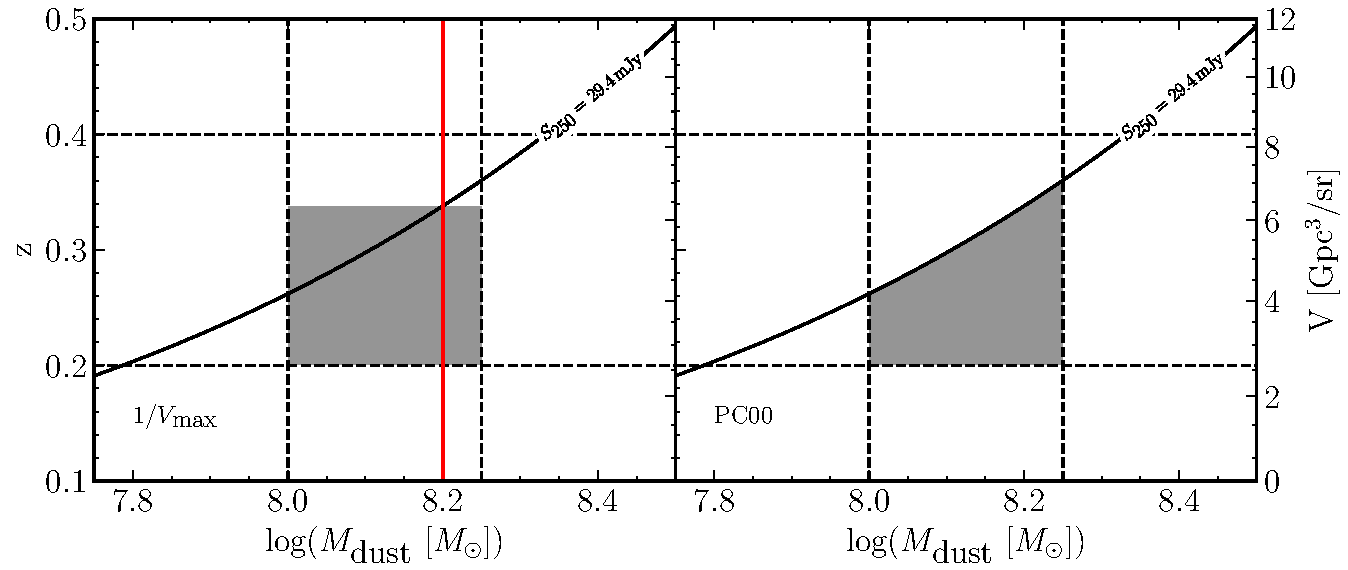
\includegraphics[width=\columnwidth]{Figures/volume_comparison.pdf}
	\caption[Example dust mass - redshift bin for the $1/V_{\textrm{max}}$ and PC00 methods]{An illustration of the accessible volume calculated in the $1/V_{\textrm{max}}$ (left panel) and PC00 methods (right panel), using Equations \ref{eq:volume_1/v_method} and \ref{eq:volume_pc00_method} respectively. Having defined an example dust mass - redshift bin ($8 < \textrm{log}(M_{\textrm{dust}} [M_{\odot}]) < 8.25$, $0.2 < z < 0.4$), the shaded areas in both panels represent the volume - dust mass space that is observable in a \textit{Herschel} survey with a limiting flux of $29.4\,$mJy at $250\,\mu$m. In the $1/V_{\textrm{max}}$ panel we have illustrated the volume as it would appear for an object with a dust mass of $8.2\,\textrm{log}(M_{\odot}$).}
	\label{fig:volume_comparison}
\end{figure}

\section{The Dust Mass Function from Galaxies in the SGP}
\label{sec:dmf_from_sgp}

We apply the three methods described above to the galaxies observed in the H-ATLAS SGP field. It is important to note that our sample is without spectroscopic redshifts and our dust masses are derived from sub-mm fluxes that are susceptible to flux boosting. The resulting scatter in the dust masses and redshifts could move galaxies between neighbouring bins. Given that the volume density is not uniform across bins and the survey is flux-limited, this introduces an Eddington bias (\citealt{Eddington_1913}) that broadens the DMF. For this reason, we model the errors as being formed in two parts. First, a Poissonian error that scales as $\sigma_{\phi,N} \propto \frac{1}{\sqrt{N}}$, where $N$ is the number of galaxies in each bin. The second error term is due to the spread in dust masses as a result of the large uncertainties on our photometric redshifts (see Section \ref{sec:phot_z_VIKING}). When measuring the DMF we run $1000$ Monte Carlo simulations in which we remeasure the DMF having perturbed the redshift of each galaxy according to a Gaussian distribution centered on the assumed redshift and with standard deviation equal to the error value. This gives us a 3D array ($M_{\textrm{dust}} - z - n$, where $n$ is the number of Monte Carlo interations) of $\phi$. We take the standard deviation along the $n$ axis, $\sigma_{\phi,z}^2$, and add this error in quadrature to the Poissonian error: $\sigma_\phi = \sqrt{\sigma_{\phi,N}^2 + \sigma_{\phi,z}^2}$.

Figure \ref{fig:dmf_methods} shows the DMFs derived using the PC00 (solid lines) and $1/V_{\textrm{max}}$ (dashed lines) methods for five redshift bins of width $0.2$, assuming a universal dust temperature of $20\,$K and dust emissivity index, $\beta = 2$. As a single SED shape is being assumed for all galaxies, we must also assume a single survey flux limit - which we take to be $29.4\,$mJy at $250\,\mu$m (\citealt{Valiante_2016}). As we predicted for bins that are entirely above the flux limit of the sample, the two estimators are equivalent. Also predicted earlier was the downturn observed in the lowest dust mass bin in most redshift slices.

The low-mass end of the DMF is typically described by a powerlaw with a gradient, $\alpha$, taking values between $-2$ and $-1$. In the lowest redshift bin, we observed dust masses small enough to constrain the value of $\alpha$, finding much flatter values than general consensus, suggesting that the number density of low redshift galaxies between dust masses of $\sim 10^{5.5}\,M_{\odot}$ and $\sim 10^{7.5}\,M_{\odot}$ is near constant. In light of previous H-ATLAS studies that do not predict this behaviour, we expect that this is not a physical trend but rather an indication of an incomplete sample at the lowest masses. Given we are not using spectroscopic redshifts, we are likely missing some of these galaxies in our sample. While we cannot rule out that the DMF has a low normalization at low dust masses, as is also seen in other studies such as \citealt{Dunne_2011}, from this point onwards we shall assume that our DMFs are accurate above $\sim 10^{7.5}\,M_{\odot}$ and use the results of \citealt{Beeston_2018} to fill in the low-mass regime. The \citealt{Beeston_2018} value of $\alpha$ was measured for low redshift galaxies, but without data to constrain this value at higher redshifts, we shall assume that this value is equally appropriate in all redshift bins.

Assuming these DMFs, we observe a clear evolution in the density of high dust mass galaxies increasing with redshift. The evolution with lookback time is evident in each redshift slice, but noticeably slows by the highest redshift bin. This may suggest that there is a point in time at redshifts $\gtrsim 0.8$ where the number density of the most massive galaxies peaks. As an extension to our $\phi_{\textrm{est}}$ prediction of the DMF, we would like to be able to use the estimator of \citealt{Dunne_2011} (Equation \ref{eq:phi_pc00_dunne_method}) in which we calculate the accessible volume individually for each source. The problem we face is that this requires knowing the dust temperatures of all galaxies in our sample. While we are able to constrain the dust temperatures for a subset of our sample, as shown in Figure \ref{fig:dust_temperatures}, we cannot depend on these sources alone without introducing another incompleteness to the sample. To avoid this problem we fit a single temperature modified blackbody to all galaxies, with bounds on the cold ISM dust temperature between $15$ and $25\,$K and with a fixed $\beta = 2$. This range of temperatures was chosen as it has been shown to be a suitable range of cold dust temperatures in galaxies (\citealt{Dunne_2001, daCunha_2008, Smith_2012b, Clark_2015, Beeston_2018}). Galaxies that have well constrained peaks in the dust emission are likely to have dust temperatures within this range, and those that have insufficient far-IR data to fit an isothermal model are assumed to take a median value of $20\,$K. Approximately $40\%$ of the galaxies in our sample have temperatures constrained between $15\,$K and $25\,$K; the remaining $\sim 60\%$ retain their $20\,$K assumption. We use this set of dust temperatures to calculate $\phi_{\textrm{est, Dunne}}$ assuming an individual survey flux limit for each source. The flux limit for each galaxy is based on a minimum SNR of four. As pointed out previously in \citealt{Dunne_2011}, this estimator is not equivalent to $\phi_{1/V}$, despite the contribution to $\phi$ being calculated for each galaxy individually in both methods. In the PC00 method we still calculate an average accessible volume for each $M_{\textrm{dust}} - z$ bin, but we now define the limiting dust mass -- redshift relationship for each source based on its own SED. This means we are more precise about the flux limit of the survey but do not depend on the uncertain dust mass estimates of the \textit{Herschel} galaxies. Our estimate of $\phi_{\textrm{est, Dunne}}$ is included in Figure \ref{fig:dmf_methods} (dotted lines). The \citealt{Dunne_2011} estimator of the DMF is broadly consistent with $\phi_{\textrm{est}}$, albeit with a wider distribution of dust masses due to the wider distribution of dust temperatures.

\begin{figure}
    \centering
    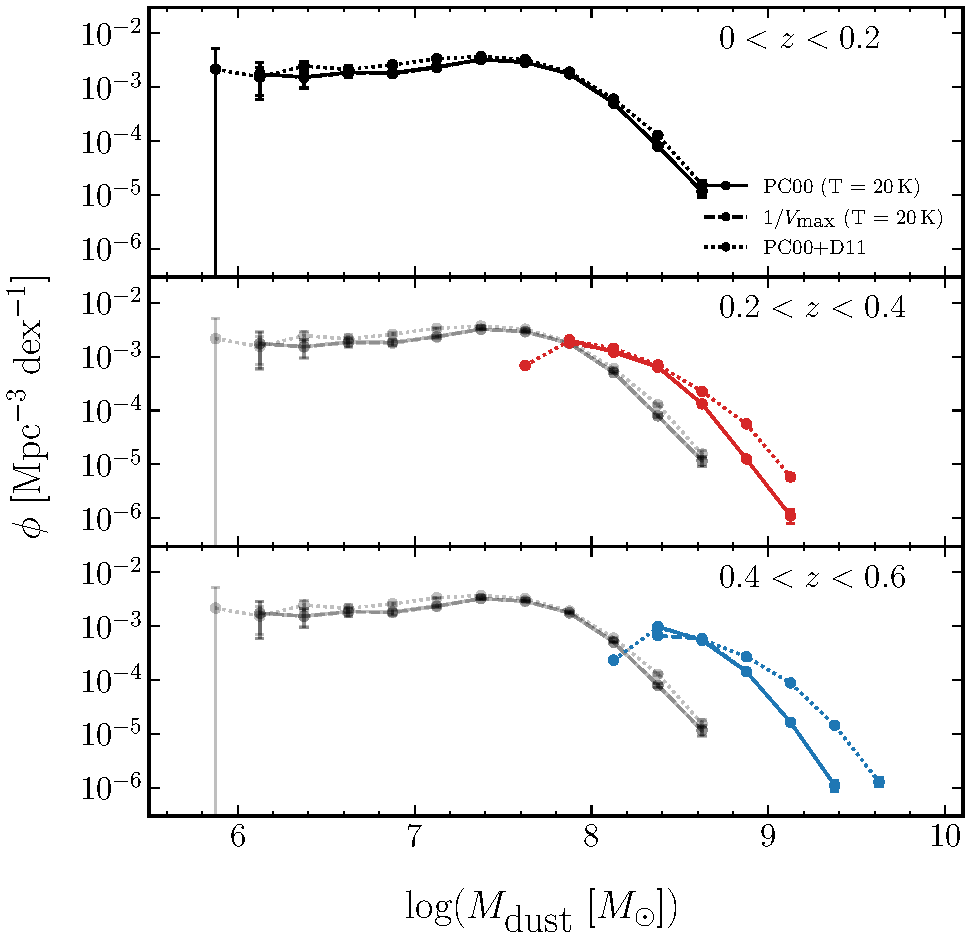
\includegraphics[width=\columnwidth]{Figures/Figure_3_4_part1.pdf}
    \caption[Dust mass functions derived from SGP galaxies]{The dust mass functions (DMFs) derived from SGP galaxies in five redshift bins of width $0.2$. The three methods described in Section \ref{sec:dmf_estimators}; the $1/V_{\textrm{max}}$, the Page and Carrera (\citealt{Page_2000}) and the Page and Carrera with the adaptation from \citealt{Dunne_2011} methods are illustrated as dashed lines, solid lines and dotted lines, respectively. In each panel the DMFs from the first redshift bin are replotted for comparison in grey. The final panel shows the DMFs from all redshift bins.}
	\label{fig:dmf_methods}
\end{figure}

\begin{figure}
    \ContinuedFloat
    \centering
    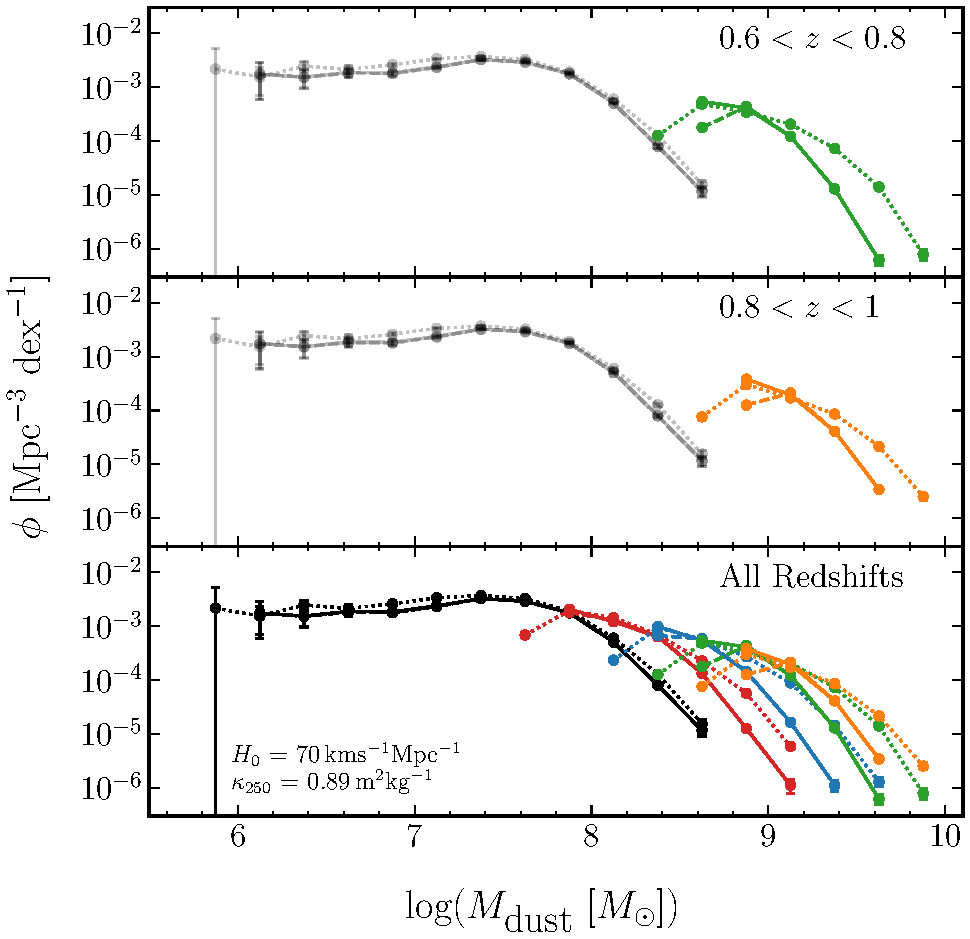
\includegraphics[width=\columnwidth]{Figures/Figure_3_4_part2.pdf}
    \caption{Continued.}
\end{figure}

\section{The Evolution in the Dust Content of SGP Galaxies}

In this section, we shall use the results of our two PC00 estimated DMFs to quantify the redshift evolution of dust mass in SGP galaxies. This is achieved in two ways: first by fitting Schechter functions to our DMFs and assessing the evolution in the Schechter parameters, and secondly, by calculating the dust mass density contained within galaxies at different epochs.

\subsection{Schechter Functions}
\label{sec:schechter_functions}

Luminosity functions, and by extension dust mass functions, are often modelled with analytical forms such as broken power laws or Schechter functions. The Schechter function takes the form

\begin{equation}
    \phi(M) dM = \phi^* (M/M^*)^\alpha e^{(-M/M^*)}\frac{dM}{M^*}
    \label{eq:schechter_function}
\end{equation}

\noindent in terms of mass, where $M^*$ is the characteristic dust mass where we transition from a power law to an exponential tail, and $\alpha$ is the exponent of the low mass power law. The normalization is defined by $\phi^*$ which corresponds to the number density of galaxies at mass $M^*$. We can convert the Schechter function to logarithmic form using the fact that $\phi(\textrm{log}(M)) = \textrm{ln}(10)M\phi(M)$ such that

\begin{equation}
    \phi(\textrm{log}(M)) d\textrm{log}(M) = \textrm{ln}(10)\phi^* e^{-10^{\textrm{log}(M)-\textrm{log}(M^*)}}\times \Bigg(10^{\textrm{log}(M)-\textrm{log}(M^*)}\Bigg)^{\alpha+1} d\textrm{log}(M).
    \label{eq:schechter_function_log}
\end{equation}

We incorporate the factor $\textrm{ln}(10)$ into our definition of $\phi^*$ such that $\phi^*$ has units of Mpc$^{-3}$dex$^{-1}$. Given the incompleteness of the lowest mass bins at high redshifts, it is common to fit the three Schechter parameters ($\phi^*$, $M^*$ and $\alpha$) for the first redshift bin and make the assumption that the value of $\alpha$ does not vary with redshift. Due to our sample incompleteness at low dust masses even in the lowest redshift slice, we fix our value of $\alpha$ to the \citealt{Beeston_2018} value of $-1.22$ throughout, and only consider values greater than $10^{7.5}\,M_{\textrm{dust}}$ in our fitting.

Figure \ref{fig:dmf_schechter} shows the best fit Schechter functions to our $\phi_{\textrm{est}}$ (solid lines, filled circles) and $\phi_{\textrm{est, Dunne}}$ (dotted lines, open circles) DMFs. The fitting parameters are listed in Table \ref{tab:schechter_parameters}. Included in Figure \ref{fig:dmf_schechter} are the studies of \citealt{Vlahakis_2005}, \citealt{Dunne_2011}, \citealt{Beeston_2018} and \citealt{Pozzi_2020}. For a direct comparison between all works we have scaled the DMFs in the literature to the same cosmology ($\Omega_m = 0.3$, $\Omega_\Lambda = 0.7$ and $H_0 = 70\,$km s$^{-1}$Mpc$^{-1}$) and dust mass absorption coefficient ($\kappa_{250} = 0.89\,$m$^{2}$kg$^{-1}$).

\begin{figure}
	\centering
	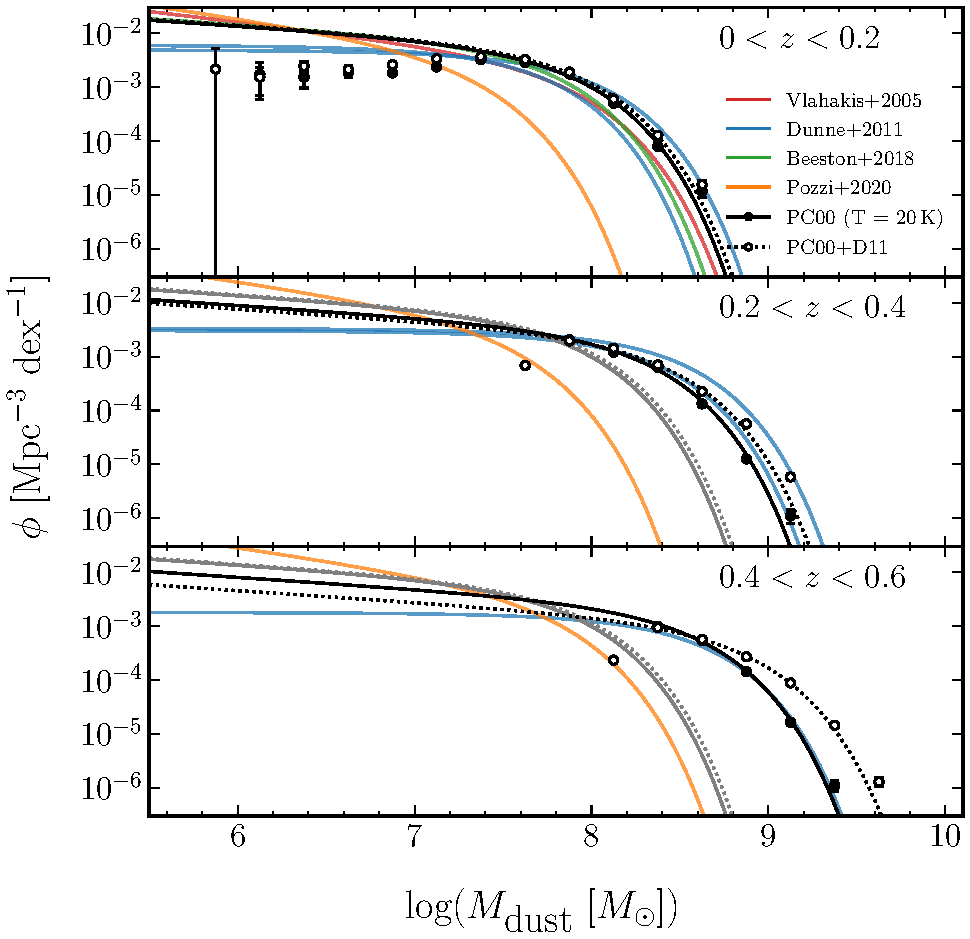
\includegraphics[width=\columnwidth]{Figures/Figure_3_5_part1.pdf}
    \caption[Schechter functions derived from the SGP DMFs alongside relevant studies]{The dust mass functions as presented in Figure \ref{fig:dmf_methods} (excluding the $1/V_{\textrm{max}}$ estimate), where the lines have been replaced with the best fitting Schechter functions (Equation \ref{eq:schechter_function_log}). The red, blue, green and orange lines represent the DMFs from \citealt{Vlahakis_2005}, \citealt{Dunne_2011}, \citealt{Beeston_2018} and \citealt{Pozzi_2020} respectively. The final panel shows the SGP DMFs from all redshift bins. The colour scales from the light to dark with increasing redshift.}
	\label{fig:dmf_schechter}
\end{figure}

\begin{figure}
    \ContinuedFloat
    \centering
    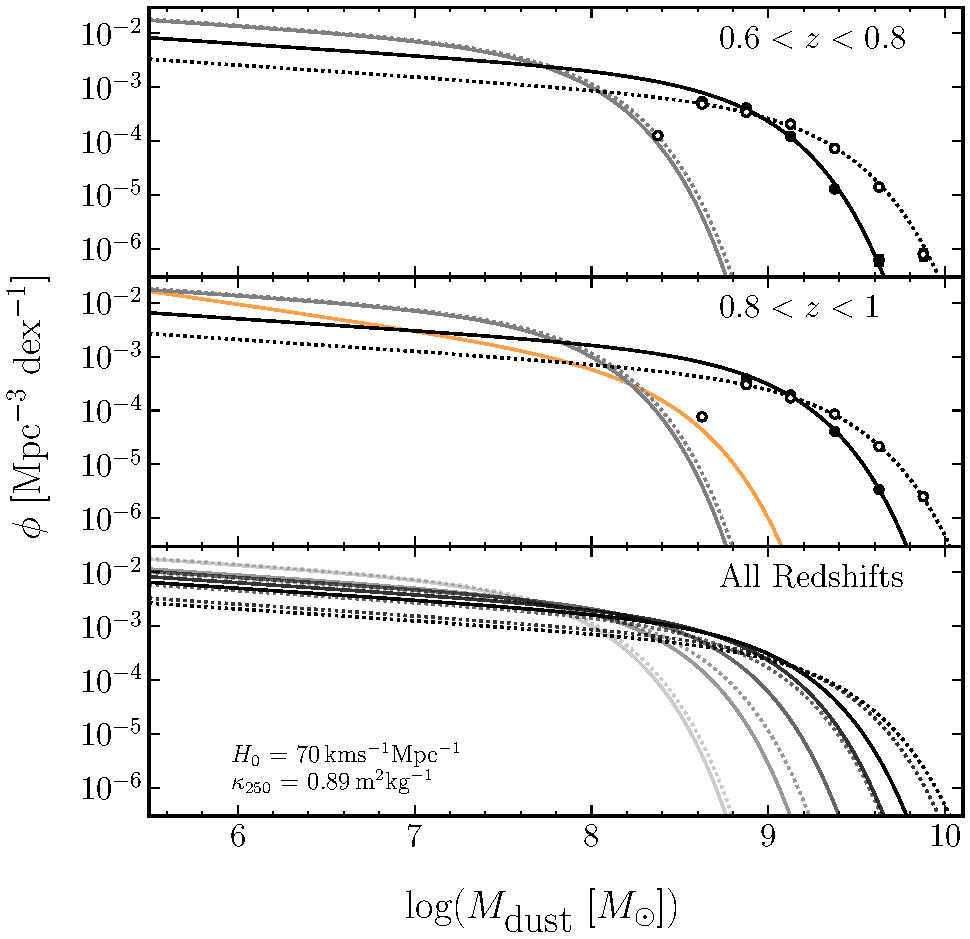
\includegraphics[width=\columnwidth]{Figures/Figure_3_5_part2.pdf}
    \caption{Continued.}
\end{figure}

\begin{table}
    \centering
    \begin{tabular}{p{1.75cm}|p{2.5cm}|p{2cm}|p{3.25cm}|p{1.25cm}|p{2cm}}
        \hline
        \hline
        Method & Redshift & log($M_{\textrm{dust}}^*$) & log($\phi^*$) & $\alpha$ & $\rho_{\textrm{dust}} (\times10^5)$ \\
        & & [log($M_{\odot}$)] & [log(Mpc$^{-3}$dex$^{-1}$)] & & [$M_{\odot}$Mpc$^{-3}$] \\
        \hline
        \hline
        \multirow{5}{*}{$\phi_{\textrm{est}}$} & 0 < z < 0.2 & $7.791^{+0.007}_{-0.007}$ & $-2.256^{+0.010}_{-0.011}$ & $-1.22$ & $1.770^{+0.051}_{-0.050}$ \\
        & 0.2 < z < 0.4 & $8.183^{+0.004}_{-0.005}$ & $-2.528^{+0.008}_{-0.008}$ & $-1.22$ & $2.331^{+0.048}_{-0.048}$ \\
        & 0.4 < z < 0.6 & $8.468^{+0.005}_{-0.005}$ & $-2.629^{+0.010}_{-0.010}$ & $-1.22$ & $3.560^{+0.088}_{-0.087}$ \\
        & 0.6 < z < 0.8 & $8.745^{+0.004}_{-0.004}$ & $-2.801^{+0.009}_{-0.009}$ & $-1.22$ & $4.542^{+0.104}_{-0.101}$ \\
        & 0.8 < z < 1 & $8.890^{+0.005}_{-0.005}$ & $-2.930^{+0.012}_{-0.012}$ & $-1.22$ & $4.695^{+0.139}_{-0.136}$ \\
        \hline
        \multirow{5}{*}{$\phi_{\textrm{est, Dunne}}$} & 0 < z < 0.2 & $7.827^{+0.007}_{-0.007}$ & $-2.249^{+0.010}_{-0.010}$ & $-1.22$ & $1.952^{+0.054}_{-0.053}$ \\
        & 0.2 < z < 0.4 & $8.305^{+0.004}_{-0.004}$ & $-2.628^{+0.006}_{-0.006}$ & $-1.22$ & $2.451^{+0.041}_{-0.040}$ \\
        & 0.4 < z < 0.6 & $8.747^{+0.005}_{-0.005}$ & $-2.943^{+0.006}_{-0.006}$ & $-1.22$ & $3.288^{+0.059}_{-0.059}$ \\
        & 0.6 < z < 0.8 & $9.117^{+0.003}_{-0.003}$ & $-3.277^{+0.003}_{-0.003}$ & $-1.22$ & $3.570^{+0.039}_{-0.039}$ \\
        & 0.8 < z < 1 & $9.195^{+0.004}_{-0.004}$ & $-3.386^{+0.004}_{-0.004}$ & $-1.22$ & $3.323^{+0.044}_{-0.044}$ \\
        \hline
    \end{tabular}
    \caption[Best fitting Schechter parameters of our SGP DMFs in each redshift slice]{The best fitting Schechter parameters for each redshift slice. The parameter $\phi^*$ incorporates the factor \textrm{ln}(10) such that it has units of Mpc$^{-3}$dex$^{-1}$. The uncertainties in the Schechter parameters are taken from the $16$th to $84$th percentiles of the posterior distribution for each parameter. The rightmost column lists the dust mass densities as calculated using Equation \ref{eq:dust_mass_density}.}
    \label{tab:schechter_parameters}
\end{table}

The local DMFs ($z < 0.2$) are in good agreement except for the low mass normalization and the offset in dust mass with the study of \citealt{Pozzi_2020}. While it is hard to reconcile the low normalizations found by our study and \citealt{Dunne_2011} with other works in the literature without a full understanding of the completeness of the respective samples at low flux densities, the shift in dust mass observed by \citealt{Pozzi_2020} in all redshift bins can be understood by comparing the selection wavelengths of the samples and their sensitivity to dust temperature. As mentioned previously, estimating dust masses from long wavelength photometry is advantageous as the Rayleigh-Jeans (R-J) part of the Planck function is least sensitive to dust temperature and most sensitive to dust mass. In the R-J regime ($\lambda_{\textrm{rest}} \gg \frac{hc}{kT}$) the Planck function reduces to $B(\nu_{250}, T) = \frac{2\nu_{250}^{2}kT}{c^2}$ which means that in the optically thin and R-J regimes our dust masses are only linearly dependent on the dust temperature.

This work, as well as the studies of \citealt{Dunne_2011} and \citealt{Beeston_2018}, are based on samples of H-ATLAS sources which are primarily selected at $250\,\mu$m. In the rest frame of the highest redshift galaxies considered here, the selection wavelength is still expected to be on the long wavelength side of the peak in dust emission. Further, at $850\,\mu$m, the SLUGS study of \citealt{Vlahakis_2005} is securely on the R-J side of the SED at the low redshifts probed in the SCUBA-selected study. As a result, these studies are sensitive to thermal emission from dust with fairly cool temperatures which should probe most of the dust mass. The $160\,\mu$m selection wavelength of \citealt{Pozzi_2020} means that in the rest frame this study probes different parts of the dust spectrum, crossing the peak to shorter wavelengths at $z \sim 0.5$. As we approach the peak of the dust SED an estimate of the dust mass becomes increasingly dependent on the measurement of the dust temperature - an effect that should also be noted when making conclusions from the highest redshift bins in our study. This is not to say that any study is inaccurate, but rather suggests that comparing studies with samples selected at different wavelengths may differ significantly, particularly if their dust temperatures are very different. It is also worth pointing out that there is a clear offset from the \citealt{Pozzi_2020} DMF even at $0 < z < 0.2$, where this effect is the least impactful, and therefore is not fully explained by this argument.

\subsection{Evolution of the Dust Mass Function}

To quantify the evolution we observe in dust masses of SGP galaxies, we can illustrate the variation in the characteristic dust mass and density in each redshift slice as obtained from our best fitting Schechter functions. Figure \ref{fig:dmf_schechter_parameters} shows the distribution of $\phi^*$ and $M_{\textrm{dust}}^*$ for our $\phi_{\textrm{est}}$ and $\phi_{\textrm{est, Dunne}}$ DMFs, as well as the studies considered in Figure \ref{fig:dmf_schechter}. We observe a strong evolution in the characteristic dust mass $M_{\textrm{dust}}^*$ with redshift, suggesting that galaxies were dustier at higher redshift. The density $\phi^*$ appears to decrease with redshift, but this is dependent on how well we account for the incompleteness in the sample. The characteristic dust mass evolves from $M_{\textrm{dust}}^* = 6.18\substack{+0.10\\-0.10}\times10^7\,M_{\odot}$ at $z < 0.2$ to $M_{\textrm{dust}}^* = 7.76\substack{+0.10\\-0.09}\times10^8\,M_{\odot}$ at $z = 0.8 - 1$, assuming a universal dust temperature of $20\,$K, suggesting a factor of $\sim 13$ in dust mass between the highest and lowest redshift bins. If we allow the $\sim 40\%$ of galaxies with well constrained dust temperatures to define their own K-corrections, then we observe a much steeper evolution from $M_{\textrm{dust}}^* = 6.71\substack{+0.10\\-0.10}\times10^7\,M_{\odot}$ to $M_{\textrm{dust}}^* = 1.57\substack{+0.01\\-0.02}\times10^9\,M_{\odot}$ over the same time period. This implies a factor increase twice as large compared to our $T_{\textrm{dust}} = 20\,$K DMF.

\begin{figure}
	\centering
	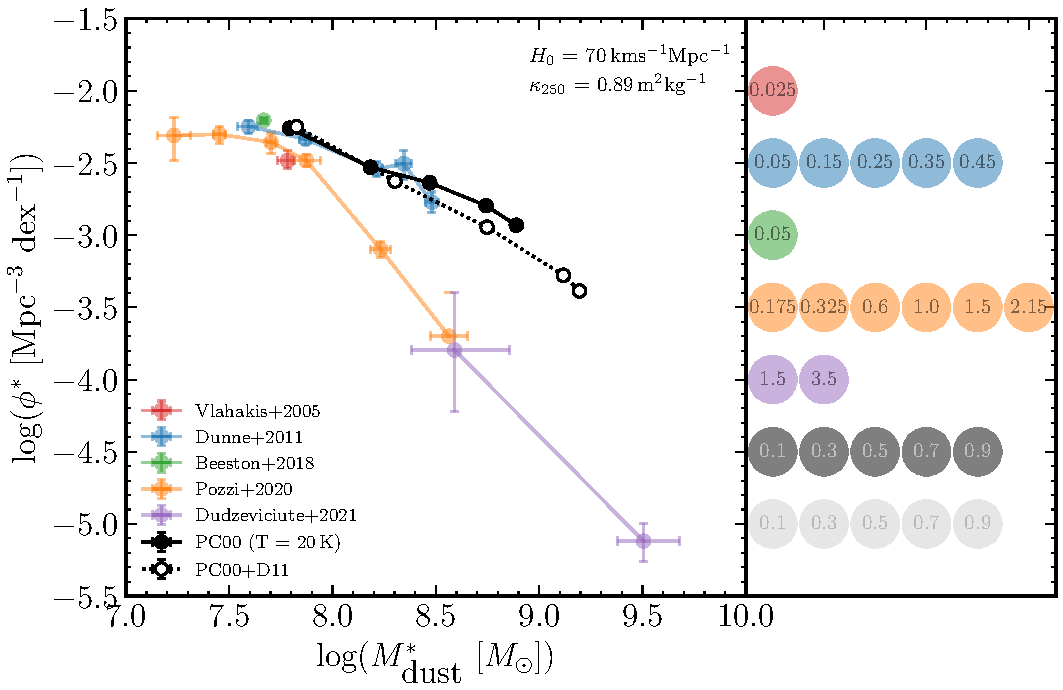
\includegraphics[width=0.9\columnwidth]{Figures/Figure_3_6.pdf}
	\caption[Distribution of $M_{\textrm{dust}}^*$ and $\phi^*$ from best fitting Schechter functions]{Left panel: The distribution of $M_{\textrm{dust}}^*$ and $\phi^*$ for the two estimates of the DMF considered in this study ($T = 20\,$K shown as filled circles with solid lines and the \citealt{Dunne_2011} adaptation shown as open circles with dotted lines). The studies from the literature are the same as those given in Figure \ref{fig:dmf_schechter}. Right panel: The center of each redshift interval for the measurements travelling left to right in the lefthand panel.}
	\label{fig:dmf_schechter_parameters}
\end{figure}

Figure \ref{fig:dmf_m_evolution} shows the variation in the characteristic dust mass as a function of redshift. We fit the observed relationships with a function of the form $\textrm{log}(M_{\textrm{dust}}^*) = \textrm{log}(M_{\textrm{dust,0}}^*)(1+z)^\gamma$. The best fitting functions are given by $\textrm{log}(M_{\textrm{dust}}^*) = (7.66\pm0.10)(1+z)^{0.30\pm0.03}$ when dust temperature is allowed to be free between $15$ and $25\,$K, and $\textrm{log}(M_{\textrm{dust}}^*) = (7.65\pm0.05)(1+z)^{0.24\pm0.01}$ when assuming $T_{\textrm{dust}} = 20\,$K. The $\textrm{log}(M_{\textrm{dust,0}})$ term represents a typical galaxy's dust mass at redshift zero, which is in excellent agreement between the two models. Using these fitted relationships we find that at $z = 1$, the galaxies detected by \textit{Herschel} were typically $60$ times dustier (or $\sim 25$ times when assuming $T_{\textrm{dust}} = 20\,$K) than today. \citealt{Dunne_2011} found that the most massive galaxies at the highest redshifts probed in their study, $z \sim 0.5$, have dust masses a factor of $5$ to $8$ larger than those at $z \sim 0$. At the same redshift, our empirical relationships find that the characteristic dust mass evolves by a factor of $6 - 10$, in good agreement with \citealt{Dunne_2011}.

\begin{figure}
	\centering
	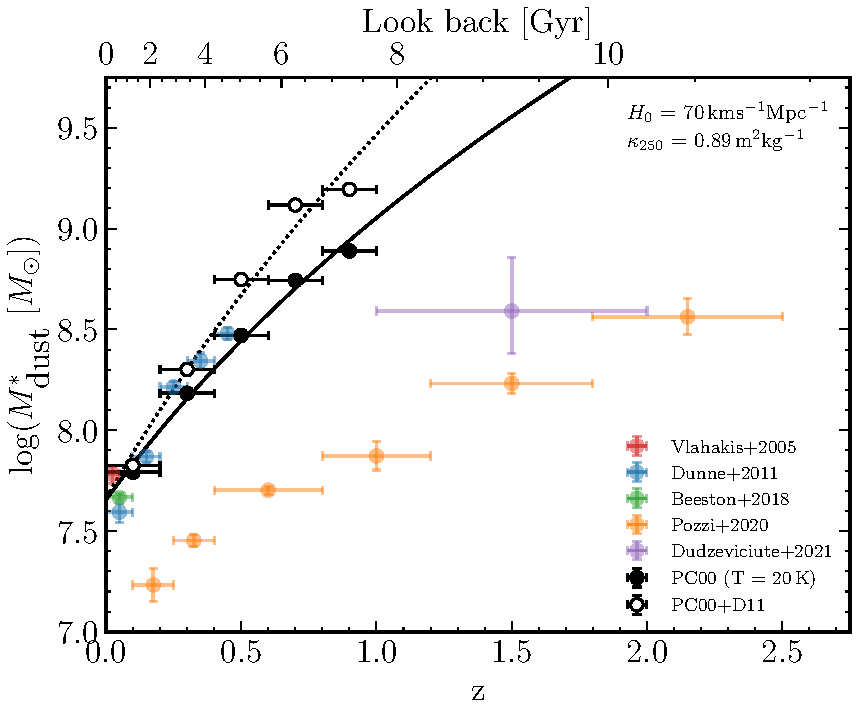
\includegraphics[width=0.7\columnwidth]{Figures/Figure_3_7.pdf}
	\caption[Evolution of the characteristic dust mass, $M_\textrm{dust}^*$, as a function of redshift]{The best fitting characteristic dust mass, $M_\textrm{dust}^*$, as a function of redshift. The coloured error bars have the same colour convention as Figure \ref{fig:dmf_schechter}. The solid and dotted lines represent best fitting relationships of the form $\textrm{log}(M_{\textrm{dust,0}}^*)(1+z)^\gamma$. For our $T_{\textrm{dust}} = 20\,$K DMF we find $\gamma = 0.24\pm0.01$ and $\gamma = 0.30\pm0.03$ when temperature is allowed to be free between $15\,$K and $25\,$K.}
	\label{fig:dmf_m_evolution}
\end{figure}

\subsection{Dust Mass Density}

Useful estimators of the dust content of galaxies across time are the integrated dust mass density (DMD), $\rho_{\textrm{dust}}$, and the dust mass density parameter, $\Omega_{\textrm{dust}}$. We integrate the DMFs in each redshift slice to calculate the total amount of dust in galaxies at different epochs. This integration is given by

\begin{equation}
    \rho_{\textrm{dust}} = \int_0^\infty M_{\textrm{dust}} \phi(M_{\textrm{dust}}) dM_{\textrm{dust}} = \Gamma(2+\alpha) M_{\textrm{dust}}^* \phi^*,
    \label{eq:dust_mass_density}
\end{equation}

\noindent where $\Gamma(x)$ represents the Gamma function, $\Gamma(x) = \int_0^\infty t^{x-1}e^{-t} dt$, and $\phi(M_{\textrm{dust}})$ has been substituted with the best fitting Schechter function. The dust mass density measured in this way is built upon a number of assumptions. First, it is assumed that the Schechter function is applicable at dust masses far below the range that has been directly measured. We could circumvent this problem by integrating to some common lower mass limit using the upper incomplete Gamma function, $\Gamma(x, z) = \int_z^\infty t^{x-1}e^{-t} dt$, however, all the studies considered here have varying levels of completeness at low masses and the integrated density without imposing this limit is negligibly different. As such, the DMD calculated using Equation \ref{eq:dust_mass_density} serves as a maximal estimate of the dust mass density. Second, the low mass slope is assumed to be constant with redshift such that the number density of lower mass galaxies does not change with time. This assumption has no motivation, but is not expected to have a significant impact on our dust mass densities as the majority of the contribution by mass comes from the much fewer, more massive galaxies. The dust mass density parameter is obtained from $\Omega_{\textrm{dust}} = \rho_{\textrm{dust}}/\rho_{\textrm{crit}}$ where $\rho_{\textrm{crit}} = 1.36\times10^{11}\,M_{\odot}$Mpc$^{-3}$ is the critical density for our assumed cosmology. The dust densities are listed in Table \ref{tab:schechter_parameters} and shown in Figure \ref{fig:dmd} alongside the measured values for the studies previously mentioned. 

\begin{figure}
	\centering
	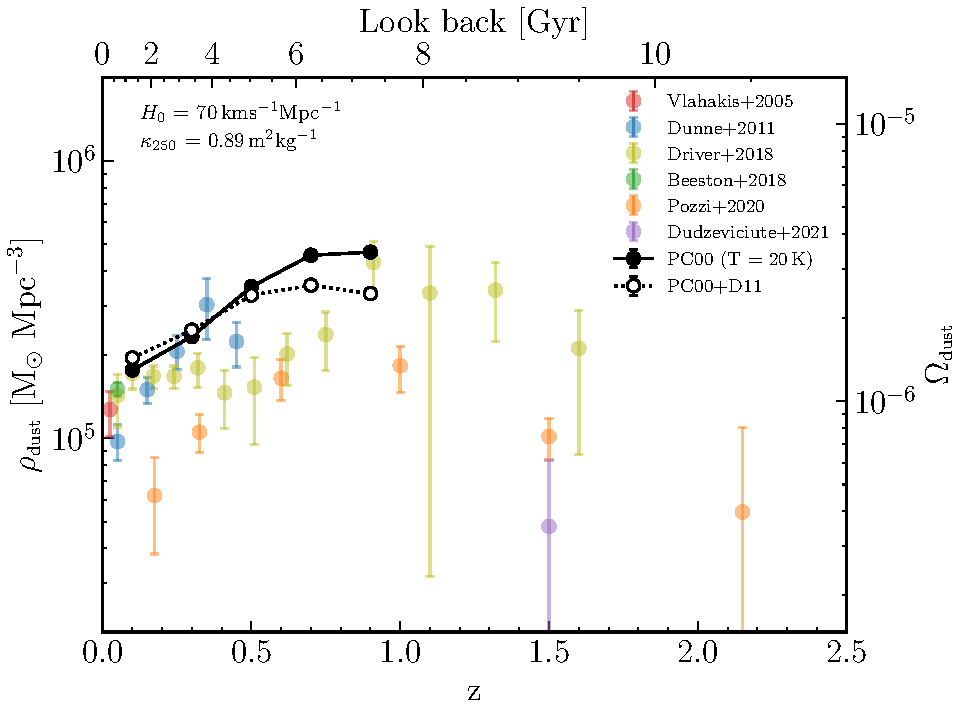
\includegraphics[width=0.8\columnwidth]{Figures/Figure_3_8.pdf}
	\caption[Integrated dust mass density as a function of redshift]{The integrated dust mass density and dust density parameter as a function of redshift for SGP galaxies, calculated using Equation \ref{eq:dust_mass_density}. The coloured error bars have the same colour convention as Figure \ref{fig:dmf_schechter}, with the addition of the study of \citealt{Driver_2018} (light green).}
	\label{fig:dmd}
\end{figure}

In reasonable agreement with \citealt{Dunne_2011}, we predict a rapid evolution in dust mass density in the local Universe, though it is notably less steep than the $(1+z)^{4.5}$ relationship observed in their study. Our measurement of the dust mass density suggests a factor $\sim 1.7 - 2.6$ increase between $0 < z < 0.2$ and $0.8 < z < 1$, beyond which the dust density remains roughly constant, suggesting a peak at redshifts around $0.8 - 1$. The rapid decrease in dust density from $z \sim 1$ to the present day may have a number of possible causes. First, the depletion of dust due to star formation, owing to the fact that evolution in dust mass and SFR are intrinsically related since stars form out of gas and the dust is expected to trace the interstellar gas reservoir. The decline may also be attributed to dust destruction or dust lost from the galaxy to the halo (\citealt{Dunne_2011}). In contrast to the prevailing \textit{Herschel} view, \citealt{Driver_2018} find a relatively flat density at redshifts $< 0.5$, though it is noted that the method used to calculate the incompleteness in their sample differs from the one used here, and by extension in \citealt{Dunne_2011}, which may be the root cause of the difference.

The prediction of a peak in the dust density varies among studies. \citealt{Driver_2018} study the stellar mass and dust mass density of GAMA sources out to redshift five, probing a large span of cosmic time and locating a peak in the dust density at $z \sim 1$. Despite an increase in the characteristic dust mass, \citealt{Dunne_2011} also observe a peak in their last redshift bin ($0.4 < z < 0.5$), however, this is based on a single dipped bin and has been linked to a systematic issue with photometric redshifts. Our two DMFs show signs that there is a peak in the dust density at a similar cosmic time to that of \citealt{Driver_2018}, but is also based on a single lower bin. In our study we only use photometric redshifts, but have factored the additional uncerainty this creates in our DMFs by running Monte Carlo simulations (Section \ref{sec:dmf_from_sgp}). We find that the contribution to the error budget from using photometric redshifts is of order the Poissonian errors and do not have a significant effect on the Schechter fitting and resulting dust mass densities. If, however, there were a systematic trend in the photometric redshifts, we might expect the observed evolution to change in steepness and/or shift the apparent peak to different redshifts.

\subsection{Comparison with the Star Formation Rate Density}

There is a direct link between star formation and the dust and gas content of galaxies. The Kennicutt-Schmidt relationship demonstrates the link between the gas and star formation rate surface densities of galaxies. Given that dust traces the gas in the ISM, there is a consequential link between dust content and the star formation activity. As a result, it is constructive to look at the dust mass density we observe from the galaxies in the SGP with the mean star formation rate in the Universe.

The redshift dependence of the cosmic star formation history given by \citealt{Madau_2014}, which takes the form of a double power law in $(1 + z)$, is based on the best fit to multiple UV and IR data sets representing the unobscured and obscured star formation densities. Combining these surveys provides a clear and comprehensive picture of the cosmic star formation activity. The best fitting function is given by

\begin{equation}
    \psi(z) = 0.015\frac{(1+z)^{2.7}}{1+[(1+z)/2.9]^{5.6}} [M_{\odot}\textrm{yr}^{-1}\textrm{Mpc}^{-3}].
    \label{eq:madau_sfrd}
\end{equation}

This expression implies a cosmic star formation history that scales as $(1 + z)^{-2.9}$ between $3 \lesssim z \lesssim 8$, a peak in the range $1.5 \lesssim z \lesssim 2$, and a decline of the form $(1 + z)^{2.7}$ to the present day. Figure \ref{fig:sfrd} shows our measurements of the dust mass density alongside the measurements of the mean star formation rate in the Universe. The offset between the two scales has been set to follow the relationship $\rho_{\textrm{dust}} = \rho_{\textrm{gas}}/\delta_{\textrm{gdr}} \sim \psi \times\tau_{\textrm{depl}}/\delta_{\textrm{gdr}}$, where we have assumed a typical depletion timescale, $\tau_{\textrm{depl}}$, of $1\,$Gyr (which is of a similar magnitude to individual galaxies on the star forming main sequence with $\textrm{log}(M_*) = 10.5$ at $z < 1$, as presented in \citealt{Tacconi_2020}) and a gas mass to dust mass ratio, $\delta_{\textrm{gdr}}$, of $100$. However, we do not intend for this to be interpreted as a suitable definition for the star formation density of SGP galaxies, rather as an approximation such that the two sets of measurements roughly coincide. 

\begin{figure}
	\centering
	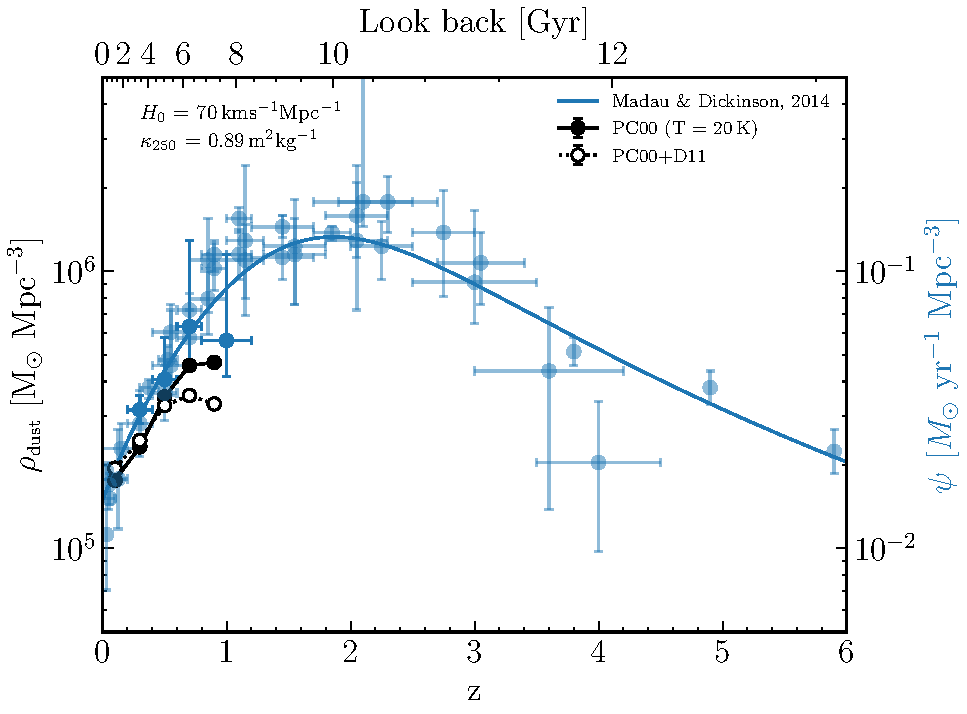
\includegraphics[width=0.74\columnwidth]{Figures/Figure_3_9.pdf}
	\caption[Comparison of dust mass density and the cosmic star formation rate density]{The integrated dust density of SGP galaxies as illustrated in Figure \ref{fig:dmd}. The blue error bars represent the various studies included in the fitting of \citealt{Madau_2014} for the cosmic star formation rate density (blue line). The two vertical axes have been scaled for illustrative purposes using $\rho_{\textrm{dust}} \sim \psi \times\tau_{\textrm{depl}}/\delta_{\textrm{gdr}}$, where we have assumed a typical depletion timescale of $500\,$Myr and a gas mass to dust mass ratio of $100$.}
    \label{fig:sfrd}
\end{figure}

The similarity in the evolutions of the dust mass density and the star formation rate density (SFRD) to the present day show that the two are intrinsically linked, and that the quantity of dust contained in galaxies is dependent on recent star formation. We know that dust can be formed in several ways, each with appreciably different timescales: the stellar winds of evolved asymptotic giant branch (AGB) and red giant branch (RGB) stars, which dominate dust production in high redshift galaxies for $150$ to $500\,$Myr after the onset of star formation (\citealt{Valiante_2009}); supernovae that dominate on timescales $< 1\,$Gyr (\citealt{Dwek_2007}); and continual grain growth in the ISM. Most processes involving dust can be linked directly to star formation, such as the formation of molecular clouds, stellar ejecta and supernovae, which all operate on timescales of order of the lifetime of massive stars (approximately less than $10\,$Myr, \citealt{Galliano_2018}). This means that it is not necessarily surprising that our dust mass density and the star formation rate density evolve in unison. Such short timescales would imply that the tentative peak in our evolution of $\rho_{\textrm{dust}}$ at $z \sim 1$, approximately $2 - 3\,$Gyr away from the peak in star formation density, is the result of some bias related to our use of photometric redshifts in estimating dust masses, but if true, would suggest a preference for dust production pathways that allow for a noticeable delay between the onset of star formation and dust production.

\section{Conclusions}

In this Chapter, we derived the dust masses of our SGP galaxies assuming an isothermal modified blackbody, setting limits on the temperature of the cold dust reservoir between $15$ and $25\,$K. From our sample we derived binned dust mass functions in redshift slices out to $z = 1$, representing approximately $8$ billion years in the past. We explored the differences between two measures of the DMF; one in which the cold dust is assumed to be constant at $20\,$K for all galaxies, and one where the dust temperature was allowed to vary within the predetermined bounds. The two methods yield similar results and are presented together without preference. From the evolution in the characteristic dust mass, we estimated that \textit{Herschel} detected galaxies were on average $25$ to $60$ times dustier at $z = 1$ than they are today. Next, we integrated both DMFs for the total amount of dust in \textit{Herschel} galaxies at various points in time. This dust mass density showed a rapid evolution from $z = 1$ to $z = 0$ of a factor approximately half, suggesting significant dust depletion due to star formation, dust destruction or dust lost to the halo over the past $8\,$Gyr. There is tentative evidence of a peak in the dust mass density at redshifts between $0.8$ and $1$, which if true, is shifted by $2 - 3\,$Gyr from the peak in the star formation rate density at $z \sim 2$. However, the most plausible cause of this downturn is our reliance on photometric redshifts that may have a systematic bias in this bin.



\chapter{Dust Properties of IR-bright, Star Forming Galaxies}
\label{chapter:Dust_Evolution}
\sloppy

\section{Introduction}

Molecular hydrogen, $H_2$, is the primary fuel for star formation (\citealt{Kennicutt_2012}) and the most abundant molecule in the Universe. The large star formation rates of DSFGs suggest that they should contain large masses of molecular gas, however, this is difficult to observe directly unless originating from energetic environments. Alternatives to observing $H_2$ directly involve taking observations of a tracer of the gas, then estimating the gas mass from the luminosity of this tracer and via a calibration between the two. Tracers that have been used in the past include the CO molecule, dust grains and carbon atoms (e.g. \citealt{Dunne_2022}). Studies using dust as a tracer of the gas in high redshift galaxies (e.g. \citealt{Magdis_2012, Eales_2012, Scoville_2014, Santini_2014, Genzel_2015}) have shown that galaxies at high redshift contain a higher fraction of gas than observed in galaxies today (\citealt{Tacconi_2010, Scoville_2016, Scoville_2017, Millard_2020}). While an important finding, we note that the dust calibration factors used during these studies are based on observations of our own Galaxy, and thus make the basic assumption that physical and chemical properties of the interstellar dust remain constant with redshift. Thankfully, recent observational (e.g. \citealt{Shapley_2020, Popping_2022}) and theoretical (e.g. \citealt{Popping_2017, Li_2019}) studies have suggested that the dust-to-gas mass ratio appears not to evolve with redshift.

A useful indicator of the physical and chemical properties of the dust is the dust emissivity spectral index, $\beta$, which controls the frequency dependence of the emissivity of the dust grains. The optical depth of the dust in a galaxy can be approximated as a power law of the form $\tau \propto \nu^\beta$, where theoretical models for dust (e.g. \citealt{Draine_1984, Draine_2011, Kohler_2015}) predict $\beta$ values to range between $1 - 2$ depending on the chemical composition. While the Galactic value is uniformly found to be $\beta = 1.51\pm0.01$ (\citealt{Planck_Collaboration_2015}), recent studies have shown that the value of $\beta$ can take a wide variety of values within local galaxies, and often within regions of the same galaxy. For example, \citealt{Lamperti_2019} modelled the far-IR SEDs of 192 nearby galaxies from the \textit{JCMT dust and gas in Nearby Galaxies Legacy Exploration} (JINGLE) survey and observed a range of $\beta$ values between $0.6$ and $2.2$, while studies of M31 and M33 (e.g. \citealt{Smith_2012, Draine_2014, Tabatabaei_2014, Whitworth_2019, Athikkat-Eknath_2022, Clark_2023}) have identified a decreasing radial trend of $\beta$, potentially a result of $\beta$ evolving to higher values in denser regions of the ISM due to grain coagulation. In this work, we test the assumption that the properties of dust are the same at all times in cosmic history by investigating whether there is evidence for evolution in the dust temperature and, importantly, the dust emissivity index, for a sample of DSFGs selected by \textit{Herschel} and SPT between $z = 2$ and $z = 6$.

\section{Obtaining Redshifts from Carbon Monoxide Lines}

In order to study the evolution of the dust properties of DSFGs we require robust redshifts to place their formation in cosmic history and to determine accurate measurements of fundamental properties. Robust measurements of a galaxy's redshift is hampered by the poor spatial resolution of single-dish observations, as their dust-obscured nature makes the identification of the counterparts at wavelengths where spectroscopically determined redshifts are readily available more difficult.

A more direct way of obtaining redshifts for low resolution far-IR/sub-mm sources, is to observe molecular emission lines which can be directly associated with the sub-mm emission without the need for intermediary steps with high-resolution imaging to locate the source of the dust emission. Recent advancements in instruments like ALMA and the Northern Extended Millimetre Array (NOEMA) allow us to detect spectral lines from molecules such as CO and [CII], that emanate unambiguously from the sub-mm source. CO is the second most abundant molecule in the Universe after $H_2$ (\citealt{Glover_2011}) and has rotational transitions that produce some of the brightest lines in the millimeter spectrum (\citealt{Rickard_1975}). The brightness of the CO lines result from the abundance of CO, the low excitation energy of the transitions and the wavelengths at which they occur coinciding with regions of the spectrum with high atmospheric transmission probed by ALMA. An additional advantage of using molecular emission to determine spectroscopic redshifts is that they are independent of the photometry used to describe the thermal dust SED and are therefore less prone to bias. In Figure \ref{fig:redshift_ladder} we show the coverage of CO line transitions as functions of redshift and observed frequency, covering the frequency range probed by the band-3 receiver of ALMA (\citealt{Weiss_2013}). The figure shows that there is non-uniform coverage of CO transitions, with some regions where multiple line detections are possible, allowing for unambiguous constraints on the redshift of the galaxy, single detections, leaving the possibility of ambiguity to the redshift solution, and redshift deserts. In this work, we study bright infrared sources detected by \textit{Herschel} and the South Pole Telescope (SPT; \citealt{Carlstrom_2011}) that have spectroscopically determined redshifts from molecular line emission, to test whether their measured dust properties evolved from the early Universe to the peak epoch of star formation ($2 \lesssim z_{\textrm{spec}} \lesssim 6$). 

\begin{figure}
	\centering
	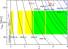
\includegraphics[width=0.8\columnwidth]{Figures/redshift_ladder.pdf}
	\caption[Spectral coverage of molecular emission lines]{The spectral coverage of CO, [CI] and H$_2$O emission lines as a function of redshift, showing the expected frequencies of lines in the region covered by ALMA's band-3 receiver. The green regions represent redshift windows where more than one line can be detected and yellow regions represent the redshifts where only one line can be detected. This figure was initially presented in \citealt{Weiss_2013}.}
	\label{fig:redshift_ladder}
\end{figure}

\section{Sample Creation}

The set of galaxies studied here is a combination of two separate samples; the South Pole Telescope - Sunyarv-Zel'dovich (SPT-SZ) survey (\citealt{Vieira_2010, Mocanu_2013, Everett_2020}) and the \textit{Herschel} Bright Sources (HerBS; \citealt{Bakx_2018}) catalogue. The following sections outline the redshift surveys, photometric coverage and restrictions imposed to produce our final sample of galaxies.

\subsection{South Pole Telescope DSFGs}

A population of IR-bright SMGs selected at $1.4\,$mm were obtained from the SPT-SZ survey which covers approximately $2,500\,$deg$^2$. The depth of this survey reaches $\sim 20\,$mJy at $1.4\,$mm. The sample of $81$ DSFGs presented in \citealt{Weiss_2013}, \citealt{Strandet_2016} and \citealt{Reuter_2020} also required a flux density above $25\,$mJy at $870\,\mu$m from APEX-LABOCA. We take as our SPT sample the same $81$ DSFGs presented in these studies.

The high flux density cuts imply that most IR-bright galaxies would not be intrinsically bright enough to be detected in this sub-sample without having been magnified from gravitational lensing. As shown by \citealt{Reuter_2020}, the average magnification of these sources is $\mu \sim 5.5$ corresponding to intrinsic flux densities similar to the flux densities of unlensed sources identified from blank field surveys at sub-mm/mm wavebands (e.g. \citealt{Coppin_2006, Pope_2006, Weiss_2009}), and are thus likely to be representative of this population albeit at higher observed redshifts.

During ALMA Cycle 0 \citealt{Weiss_2013} conducted a blind redshift survey for $26$ SPT sources with ALMA's band 3 receiver ($2.6 - 3.6\,$mm). In total, $44$ line features were identified from $^{12}$CO, $^{13}$CO, [CI], H$_2$O and H$_2$O$^+$. $12$ sources had spectra with multiple clear line features, from which a unique redshift solution could be found from the ALMA scans alone; $11$ had a single line feature for which other spectroscopic or photometric measurements would be required to constrain the redshift; and three sources for which no line features were observed. The same observing strategy was used during ALMA Cycle 1 by \citealt{Strandet_2016} to extend the redshift survey of \citealt{Weiss_2013} with an additional $15$ sources observed in ALMA band 3. For sources with a single CO line detection during Cycle 0, \citealt{Strandet_2016} present ALMA $1\,$mm (band 6) follow-up observations and, when still not satisfactory, follow-up observations were made with the First Light APEX Submillimetre Heterodyne receiver (FLASH; \citealt{Heyminck_2006}) and the Swedish-ESO PI receiver (SEPIA; \citealt{Billade_2012}). For those that remained unambiguous during Cycles 0 and 1, sources were observed with the Z-spec camera (\citealt{Naylor_2003}) onboard the Atacama Pathfinder Experiment (APEX) targeting CO and [CII] lines. Lastly, \citealt{Reuter_2020} concluded the SPT redshift survey during ALMA Cycles 3, 4 and 7 by presenting spectra for the remaining $40$ sources that had yet to be scanned. The culmination of these studies is a sample of $81$ SPT-selected DSFGs each with a spectroscopic redshift in the range $1.9 < z_{\textrm{spec}} < 6.9$ with a median redshift of $z_{\textrm{median}} = 3.9\pm0.2$ (\citealt{Reuter_2020}).

The SPT-DSFGs have photometric coverage that fully traces the SED peak and Rayleigh-Jeans (R-J) tail of the dust emission for all sources. Most of the SPT sample have coverage that spans at least observed wavelengths between $250\,\mu$m and $3\,$mm. This photometry includes flux densities measured at $250$, $350$ and $500\,\mu$m (\textit{Herschel}-SPIRE), $870\,\mu$m (APEX-LABOCA), $1.4$ and $2\,$mm (SPT) and $3\,$mm (ALMA). For a subset of $65$ sources, $100$ and $160\,\mu$m flux densities were measured with \textit{Herschel}-PACS. The photometric coverage of the sources covers a rest frame range of $86\,\mu$m $\lesssim \lambda_{\textrm{rest}} \lesssim 380\,\mu$m meaning that the peak of the dust emission at $\sim 100\,\mu$m is always constrained and the Rayleigh-Jeans tail is well sampled.

The complete set of photometric observations for the SPT DSFGs can be found in Appendix D of \citealt{Reuter_2020} including the estimated magnifications of each source due to gravitational lensing as measured from the lens modelling of \citealt{Spilker_2016}. In the 42 cases where a magnification could not be measured, the average value of $\mu = 5.5$ is assumed.

\subsection{The HerBS Sample}

A second sample used in this study comes from HerBS, a sample selected from the brightest high-redshift sources detected from the H-ATLAS project. Using the typical H-ATLAS SED template of \citealt{Pearson_2013}, \citealt{Bakx_2018} estimated the redshift of each source and selected those that have a measured photometric redshift $> 2$ and are observed at a $500\,\mu$m flux density $> 80\,$mJy. Initially the sample consisted of $223$ sources, but having removed nearby galaxies and known blazars (\citealt{Negrello_2010, Lopez-Caniego_2013}), the HerBS sample is reduced to 209. Presented with the catalogue are observations at $850\,\mu$m with the SCUBA-2 instrument for $203$ of these sources. Spectroscopic redshifts have been obtained for a selection of HerBS galaxies in the South Galactic Pole field, as part of the Bright Extragalactic ALMA Redshift Survey (BEARS: \citealt{Urquhart_2022, Bendo_2023, Hagimoto_2023}).

The BEARS spectral line survey started in ALMA Cycles 4 and 6 using the band 3 receiver of the Atacama Compact Array (ACA) and continued during Cycle 7 in bands 3 and 4 with the ALMA $12\,$m Array. \citealt{Urquhart_2022} targeted $85$ HerBS fields for CO line emission, presenting $71$ individual spectroscopic measurements for $62$ sources. The ALMA band 4 images with angular resolution of $\sim 2\,$arcsec revealed that only half of the fields contained just a single source, while several contained two or more objects with similar spectroscopic redshifts. This suggests either that the sources are formed from physically associated galaxies, or could be multiple images caused by gravitational lensing. For this study, we have retained the HerBS sources which are multiples in the ALMA images. In the cases where the HerBS source is deblended, we assume that the redshift of the group is the average spectroscopic redshift of all components, providing they are within $0.1$ of each other. If there is only a single redshift corresponding to one of the components (and the redshift corresponding to the integrated emission of all sources is not provided), we assumed the sources are physically connected and that the redshift of the one component is the redshift of the system. While \citealt{Bendo_2023} show that the brightest component (alphanumerically labelled A for each source) produces $< 80\%$ of the total emission at $2\,$mm, it is only in 4 fields (HerBS-56, -131, -138 and -146) that the spectroscopic redshift of a multiple system is assumed from a component that is not the brightest.

The photometry available for HerBS sources covers a similar range to the SPT sample: \textit{Herschel}-SPIRE ($250$, $350$, $500\,\mu$m), SCUBA-2 ($850\,\mu$m) and ALMA ($2$, $3\,$mm). The ALMA flux densities were serendipitously estimated from the continuum of the spectrosopic survey. We also include snapshot continuum observations in ALMA band 6 ($1.1 - 1.4\,$mm) for a selection of potentially ultra-red objects from the ALMARED survey (Jianhang Chen et al., in preparation) observed in the H-ATLAS (project 2018.1.00526.S). For sources where the reduced angular resolution of the ALMA beam resolves the HerBS source into multiple components, \citealt{Bendo_2023} report the integrated flux densities of all objects if they lie within twice the FWHM of the ALMA beam, or if they are connected by structures that are themselves detected at greater than $3\sigma$ significance. We preferentially chose to use these integrated fluxes for each HerBS source if available, or failing this, combine the flux densities of individual components providing they are all detected.

The shorter selection wavelength compared to the SPT sample leads to a lower redshift distribution; the minimum and maximum redshifts are $z_{\textrm{min}} = 1.407$ and $z_{\textrm{max}} = 4.509$, with a median redshift of $z_{\textrm{median}} = 2.6$. The minimum photometric coverage for a HerBS galaxy is between rest frame wavelengths of $\sim 97\,\mu$m and $\sim 392\,\mu$m, which allows us to constrain the thermal peak and Rayleigh - Jeans tail of all galaxies in the sample, just as we can with the SPT DSFGs. The photometric coverage of the 30 HerBS galaxies used in the final sample (Section \ref{sec:restrictions_on_sample}) has been tabulated in Appendix \ref{app:HerBS_photometry}.

\subsection{Restrictions on Sub-samples}
\label{sec:restrictions_on_sample}

Across the two sub-samples there are $143$ galaxies with a spectroscopic redshift ($81$ SPT, $62$ HerBS/BEARS). However, as we are interested in measuring the galaxy-integrated dust emissivity spectral index of each source, which is characterized by the slope of the emission on the R-J side of the Planck function, we make it a requirement of the final samples that there are at least two observations at observed wavelengths greater than $1\,$mm for each galaxy. This has the effect of reducing the final sample of galaxies studied here to $109$ ($79$ SPT and $30$ HerBS/BEARS). The median redshift of the HerBS sub-sample marginally changes from $2.6$ to $2.7$ as a result of this restriction (the median SPT redshift does not change when quoted to the same precision as above). While the fitting methods used in this study are the same for both sub-samples, we treat the two populations separately to highlight any potential differences that may result from the different selection wavelengths and flux limits. The redshift distributions of the two sub-samples is illustrated in Figure \ref{fig:spt_herbs_redshift}.

\begin{figure}
	\centering
	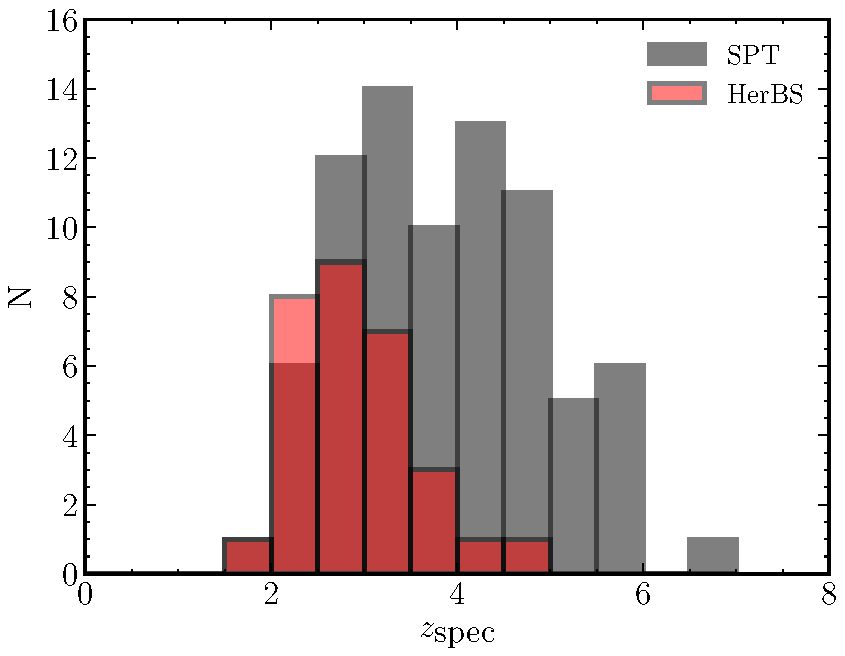
\includegraphics[width=0.8\columnwidth]{Figures/spt_herbs_redshift_distribution.pdf}
	\caption[Spectroscopic redshift distributions of HerBS and SPT-DSFG samples]{The spectroscopic redshift distributions for the SPT-DSFG (grey) and HerBS (red) samples.}
	\label{fig:spt_herbs_redshift}
\end{figure}

\section{Far-Infrared and Sub-mm Colours}
\label{sec:fir_submm_colours}

A first estimate on the average dust properties of the two samples can be made by comparing their far-IR/sub-mm colours (which we define as the ratio between two flux densities) with the predictions made using isothermal blackbody models. Previous studies have shown that far-IR colours can be useful proxies for dust properties (e.g. \citealt{Boselli_2010, Boselli_2012, Remy-Ruyer_2013, Smith_2019}) depending on the part of the far-IR spectrum that the colour samples. For example, smaller wavelengths involving the PACS and SPIRE flux densities are more sensitive to changes in the dust temperature, while longer wavelengths are more sensitive to variations in the dust emissivity spectral index. In Figure \ref{fig:spt_herbs_colour_redshift} we show a selection of colours using flux densities between $250\,\mu$m and $3\,$mm that progressively travel across the spectrum from sampling the peak of thermal dust emission to the R-J tail. Using an optically thin, isothermal modified blackbody model of the form $S_\nu \propto \frac{\nu^{\beta+3}}{e^{h \nu/kT} - 1}$, we predict the dependence of far-IR/sub-mm colour on redshift for three combinations of dust temperature, $T_{\textrm{dust}}$, and $\beta$ ([$T_{\textrm{dust}} = 30\,$K, $\beta = 2$], [$T_{\textrm{dust}} = 30\,$K, $\beta = 1.8$] and [$T_{\textrm{dust}} = 40\,$K, $\beta = 2$]). The colour-redshift plots show that the assumed dust temperature affects the location of a galaxy across all colours, while a change in the value of $\beta$ has a larger effect on the observed colours at the longest wavelengths.

\begin{figure}
    \centering
    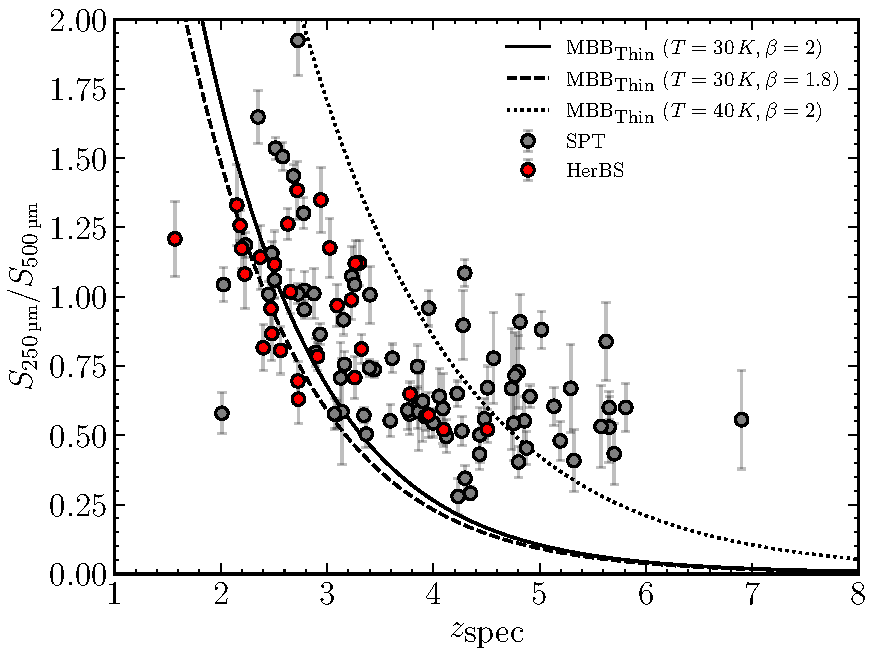
\includegraphics[width=0.55\columnwidth,height=0.29\textheight]{Figures/spt_herbs_colour_250_500.pdf}
    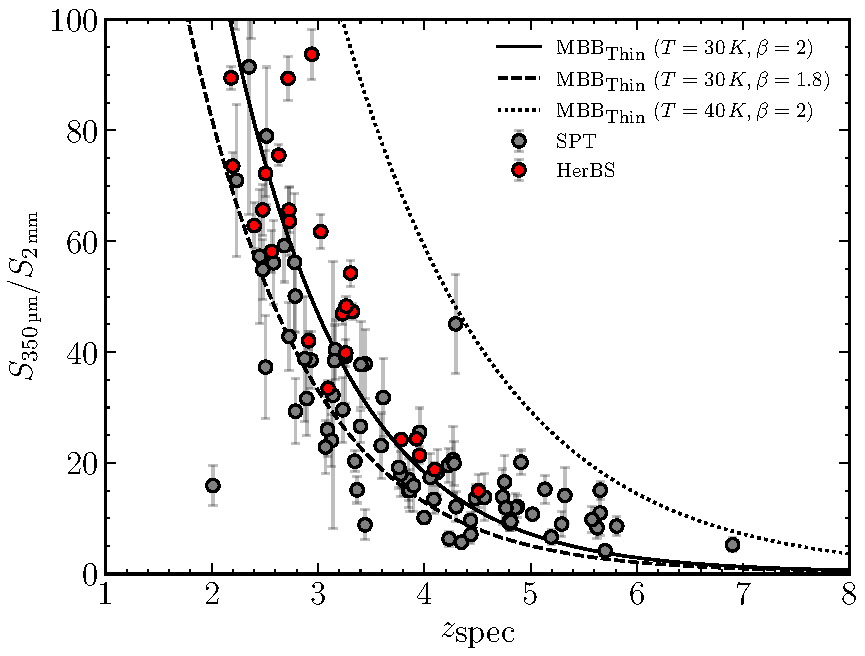
\includegraphics[width=0.55\columnwidth,height=0.29\textheight]{Figures/spt_herbs_colour_350_2000.pdf}
    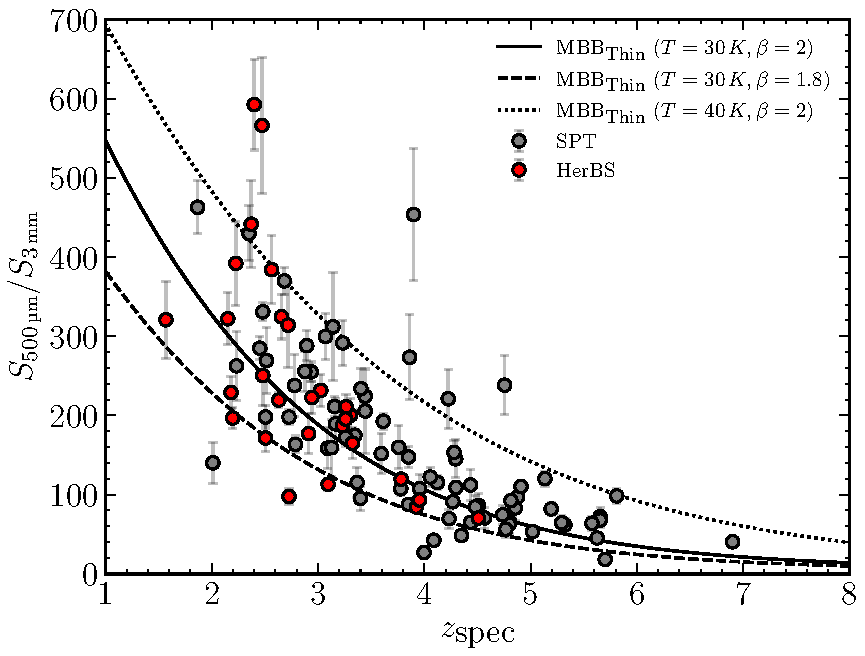
\includegraphics[width=0.55\columnwidth,height=0.29\textheight]{Figures/spt_herbs_colour_500_3000.pdf}
    \caption[Colours of HerBS and SPT sources as a function of redshift]{Colour-redshift plots of $S_{250}/S_{500}$, $S_{350}/S_{2\,\textrm{mm}}$ and $S_{500}/S_{3\,\textrm{mm}}$ against spectroscopic redshift. The SPT sources are illustrated with grey circles and the HerBS sample as red circles. The predictions from three modified blackbody models assuming optically thin dust ([$T_{\textrm{dust}} = 30\,$K, $\beta = 2$], [$T_{\textrm{dust}} = 30\,$K, $\beta = 1.8$] and [$T_{\textrm{dust}} = 40\,$K, $\beta = 2$]) are plotted as solid, dashed and dotted black lines, respectively.}
    \label{fig:spt_herbs_colour_redshift}
\end{figure}

Assuming for now that the dust emissivity index is well represented by $\beta \sim 2$ for all galaxies, then the far-IR/sub-mm colours of most sources can be explained by a range of dust temperatures between $T_{\textrm{dust}} = 30 - 40\,$K assuming optically thin dust emission. There are notable exceptions, including a selection of SPT sources with high $S_{250}/S_{500}$ and sources from both samples with high $S_{500}/S_{3\,\textrm{mm}}$. At first this might suggest sources with large dust temperatures and/or high values of $\beta$, but there are also other reasons that could be leading to deviations from the bulk population. The most likely are the uncertainties on the flux density measurements or biases due to combining photometry from different facilities. We note that our galaxies contain a combination of photometry obtained from single-dish observations (e.g. \textit{Herschel}, JCMT and SPT) and from the interferometer, ALMA. With their varying angular resolutions, emission observed with one instrument may be missed by another. In particular, we might expect that in the cases when ALMA resolves the single sources observed in the \textit{Herschel} wavebands into multiple components, some emission is lost giving the impression of higher far-IR/sub-mm colours and thus higher dust temperatures and/or higher $\beta$. In general, however, the SPT and HerBS galaxies occupy similar regions of the colour-redshift space, suggesting that the intrinsic dust properties of the two samples are likely to be similar. Given the scatter observed around the MBB models, it appears unlikely that a single value of dust temperature and $\beta$ represents the observed SED of each galaxy equally well. This would suggest that a single dust model assuming a constant $\beta$ is unlikely to explain the variety of SEDs observed among the two sub-samples. To determine an individual, galaxy-integrated $\beta$ value for each source, we must turn to fitting the observed SEDs to measure their dust properties.

\section{SED Fitting of DSFGs}
\label{sec:sed_fitting}

We model the far-IR to millimeter spectra of our galaxies by fitting a single modified blackbody model, combined with a mid-IR powerlaw, to all sources. In the far-IR to mm regime, the SED is dominated by a modified Planck function representing the cold dust found in the ISM. This cold dust resides in the diffuse ISM and is heated by the ambient interstellar radiation field. A lower fraction of dust by mass radiates at hotter temperatures, heated by nearby star-forming regions, young OB-like stars or AGNs which contribute substantially to a galaxy's IR luminosity and dominates the emission at rest frame wavelengths $\lesssim 70\,\mu$m. This mid-IR component can be approximated using a power law of dust temperatures of the form $S_\nu \propto \nu^{-\alpha}$, where low values of $\alpha$ would suggest more dust emission coming from sources other than the cold dust reservoir, and higher values asymptotically tending towards a model with a single, cold dust component.

The modified blackbody form is a direct result of the radiative transfer equation, $\frac{dI_\nu}{ds} = -\kappa_\nu \rho I_\nu + j_\nu \rho$, where $\kappa_\nu$ represents the opacity of the dust, $\rho$ is the density, $j_\nu$ represents the emissivity of the dust and $I_\nu$ is the spectral radiance (per unit area). If we define the source function, $S_\nu$ as $j_\nu/\kappa_\nu$ and the frequency dependent optical depth as $d\tau_\nu = -\kappa_\nu \rho ds$, then the radiative transfer equation becomes $\frac{dI_\nu}{d\tau_\nu} = I_\nu - S_\nu = I_\nu - B_\nu$, where we have used the fact that at local thermal equilibrium (LTE) the source function is equal to the Planck function, $B_\nu(T)$. The solution to the radiative transfer equation takes the form $I_\nu = (1 - e^{-\tau_\nu}) B_\nu(T)$. Given that the spectral radiance is proportional to the flux density at a given frequency, we can rewrite this as the modified blackbody model

\begin{equation}
	S_{\nu, \textrm{obs}} =  
	\begin{cases}
	 	\frac{\Omega}{(1+z)^3} (1- e^{-\tau_\nu}) B_\nu(T_{\textrm{dust}}), & \nu \le \nu_{\rm c} \\
	 	 N \nu^{-\alpha}, & \nu > \nu_{\rm c} \\
	\end{cases}
	\label{eq:modified_blackbody_omega}
\end{equation}

\noindent where $\Omega$ represents the solid angle subtended by the galaxy and we have included the power law form at mid-IR wavelengths. $N$ represents a normalization for the power law which is tied to the normalization of the blackbody. The value of $\nu_{\rm c}$ is the frequency at which the gradient of the MBB is equal to the value of $\alpha$. The solid angle, $\Omega$, is defined as $\frac{A(1+z)^4}{D_{\rm L}^2}$, where $A$ is the area of the source and $D_{\rm L}$ represents the luminosity distance at the redshift of the galaxy. 

The optical depth, $\tau$, is defined as the product of dust surface mass density, $\Sigma_{\textrm{dust}} = M_{\textrm{dust}}/A$ and the dust opacity, $\kappa_\nu$, but is often assumed to take the form of a power law, $(\nu/\nu_1)^\beta$, where $\nu_1$ represents the frequency at which the optical depth equals unity, and thus marks the transition between optically thick and optically thin dust. We can also describe the emissivity of the dust grains per unit mass, $\kappa_\nu$, in a similar way, using a power law of the form $\kappa_\nu = \kappa_0(\nu/\nu_0)^\beta$, where $\kappa_0$ is the emissivity of the grains per unit mass at some reference frequency $\nu_0$. Hereafter, we shall adopt $\kappa_0 = 0.077\,$m$^2$kg$^{-1}$ at $\nu_0 = 353\,$GHz ($\lambda_0 = 850\,\mu$m, \citealt{Dunne_2000, James_2002}), like we did in the previous Chapter.

Upon substituting for optical depth, we find 

\begin{equation}
	S_{\nu, \textrm{obs}} =  
	\begin{cases}
		\frac{\mu A (1+z)}{D_{\rm L}^2} \Big(1- e^{-\frac{M_{\textrm{dust}}\kappa_\nu}{A}}\Big) B_\nu(T_{\textrm{dust}}), & \nu \le \nu_{\rm c} \\
		\mu N \nu^{-\alpha}, & \nu > \nu_{\rm c} \\
	\end{cases}
\end{equation}

\noindent where we have included a term, $\mu$, accounting for the possibility of gravitational lensing. This allows us to determine intrinsic masses and luminosities. For galaxies where there is no evidence of gravitational lensing, this value defaults to $\mu = 1$.

The final amendment to the MBB models is to account for the heating of the dust due to the ambient temperature of the Cosmic Microwave Background (CMB). At high redshifts the CMB becomes a non-negligible source of heating, which unaccounted for in the model, could bias estimates of the dust temperature and dust emissivity index. When the CMB temperature at the redshift of the galaxy is a significant fraction of the cold dust temperature of the ISM within the galaxy, then we observe a change in the shape of the far-IR/sub-mm SED (\citealt{daCunha_2013}, see also \citealt{Zhang_2016} for the influence of the CMB on the measurement of structural and dynamical properties). At local thermal equilibrium, the increase in the ISM temperature due to CMB heating at higher redshifts ($T_{\textrm{CMB}} = T_{\textrm{CMB}, 0}(1+z)$, where $T_{\textrm{CMB}, 0}$ is the temperature of the CMB today, $2.72\,$K) has two competing effects on the observed dust SED. First, the dust continuum emission is boosted by the increased temperature of the CMB; and second, the increased temperature creates a stronger background from which we observe the dust continuum. The CMB-adjusted blackbody model is now given by 

\begin{equation}
	S_{\nu, \textrm{obs}} =  
	\begin{cases}
		f_{\textrm{CMB}}\frac{\mu A (1+z)}{D_{\rm L}^2} \Big(1- e^{-\frac{M_{\textrm{dust}}\kappa_\nu}{A}}\Big) B_\nu(T_{\textrm{dust}}(z)), & \nu \le \nu_{\rm c} \\
		f_{\textrm{CMB}} \mu N \nu^{-\alpha}, & \nu > \nu_{\rm c} \\
	\end{cases}
	\label{eq:modified_blackbody_general_opacity_a_cmb}
\end{equation}

\noindent where we have made two changes. First, the prefactor $f_{\textrm{CMB}}$ denotes the fraction of the total dust emission that is observed against the background of the CMB and is given by Equation 18 of \citealt{daCunha_2013}; $f_{\textrm{CMB}} = \frac{S_\nu^{\textrm{observed}}}{S_\nu^{\textrm{intrinsic}}} = 1 - \frac{B_\nu[T_{\textrm{CMB}}(z)]}{B_\nu[T_{\textrm{dust}}(z)]}$. Second, we have redefined the dust temperature to be a function of redshift, $T_{\textrm{dust}}(z)$, and is given by Equation 12 of \citealt{daCunha_2013}; $T_{\textrm{dust}}(z) = [T_{\textrm{dust}, 0}^{4+\beta} + T_{\textrm{CMB}, 0}^{4+\beta} ((1+z)^{4+\beta} - 1)]^{\frac{1}{4+\beta}}$, where $T_{\textrm{dust}, 0}$ is the dust temperature at a redshift of zero. Note that in all future references of the dust temperature of a galaxy, we refer to the luminosity-weighted, CMB-corrected temperature as defined above, unless otherwise stated.

In this general opacity form of the modified blackbody there are up to four free parameters describing the dust properties of the galaxy: the dust mass, $M_{\textrm{dust}}$, the characteristic dust temperature, $T_{\textrm{dust}}$, the radial size of the source, $r$ (which we use to define the source area, $A$), the mid-IR powerlaw index, $\alpha$, and the dust spectral index, $\beta$. As mentioned previously, some of the SPT sources have intrinsic size measurements from lens modelling in \citealt{Spilker_2016} - although caution should be exercised when using these estimates as the size is measured at a particular wavelength (in this case at $870\,\mu$m with ALMA imaging), and it is unlikely to be the same at all wavelengths due to differential lensing. We assume no differential lensing and take the effective radii as the size of the dust continuum region measured for the SPT galaxies in \citealt{Spilker_2016}. These measurements suggest that the sizes of the sub-mm emitting region is typically $\sim 1\,$kpc. All the remaining SPT and HerBS sources without known sizes require an alternative way of constraining the dust opacity. We recall the two definitions of the optical depth given above. By equating the two forms of $\tau$, $\Sigma_{\textrm{dust}}\kappa_\nu$  and $(\nu/\nu_1)^\beta$, we can find an alternative definition that reformulates the intrinsic size into an observed parameter. This is given by the transitional frequency, $\nu_1 = \nu_0 (\kappa_0\Sigma_{\textrm{dust}})^\beta = \nu_0 (\kappa_0M_{\textrm{dust}}/A)^\beta$.

We estimated the properties of the dust using three separate models. In the first, we make the simple approximation that the dust is optically thin at all wavelengths, $\tau_\nu \ll 1$, which simplifies the self opacity term from $(1 - e^{-\tau_\nu})$ to $\tau_\nu$, and removes the necessity for defining the size of the continuum emission

\begin{equation}
	S_{\nu, \textrm{obs}} =  
	\begin{cases}
		f_{\textrm{CMB}}\frac{\mu (1+z)}{D_{\rm L}^2} M_{\textrm{dust}} \kappa_\nu B_\nu(T_{\textrm{dust}}(z)), & \nu \le \nu_{\rm c} \\
		f_{\textrm{CMB}}\mu N \nu^{-\alpha}, & \nu > \nu_{\rm c} \\
	\end{cases}
    \label{eq:modified_blackbody_optically_thin}
\end{equation}

Given how high the dust masses are expected to be for the \textit{Herschel} and SPT DSFGs (and the dust is packed into a small region, e.g. \citealt{Ikarashi_2017}), it is not unreasonable to expect that the dust might be optically thick at wavelengths probed by our photometry (e.g. \citealt{Conley_2011, Casey_2019, Cortzen_2020}). For this reason, the other two models assume that dust becomes optically thick at wavelengths below $\lambda_1 = 100\,\mu$m or $200\,\mu$m (e.g. \citealt{Blain_2003, Draine_2006, Conley_2011, Rangwala_2011, Greve_2012, Casey_2014a, Spilker_2016, Casey_2019, Cooper_2022, Drew_2022}). The SPT sources that have size measurements have an additional model using the derived value of $A$, which is used as a means of comparison.

The lensing magnifications, $\mu$, are required to calculate the intrinsic mass and luminosity of the dust. For the SPT DSFGs we take the lensing magnifications to be those quoted in the lens modelling of \citealt{Spilker_2016}. For HerBS, \citealt{Urquhart_2022} estimated $\mu$ from the well studied correlation between CO luminosity, $L^{'}_{\textrm{CO}}$, and line width, $\textrm{FWHM}$ (e.g. \citealt{Bothwell_2013, Dannerbauer_2017, Neri_2020}). The logic of this method is that the CO luminosity of a source will be increased as a result of the effects of gravitational lensing, but the line width of the CO emission line will not, leading to an offset from other, unlensed sources. This offset was used to estimate the magnification factors of each of the HerBS galaxies. It should be noted, however, that these values hide an uncertainty coming from the scatter in the correlation created by the chosen unlensed sample. For the HerBS sources in this study, the magnification factors are in the range $1 - 50$ and the median is $\mu_{\textrm{median}} = 5.3$. The SPT-DSFGs range in magnification factors from $1$ to $33$, with a median value $\mu_{\textrm{median}} = 5.5$, which is assumed for all SPT sources not included in the study of \citealt{Spilker_2016}. 

During the SED fitting we assumed flat priors on all the free parameters and added calibration errors in quadrature with the flux density uncertainties at each wavelength, in the same manner as we described in Section \ref{sec:phot_z_Herschel}. We assumed absolute calibrations of $7\%$ (\textit{Herschel}-PACS), $5.5\%$ (\textit{Herschel}-SPIRE), $5\%$ (SCUBA-2), $12\%$ (APEX-LABOCA), $7\%$ (SPT) and $10\%$ (ALMA). The best fitting SED was determined from a Markov Chain Monte Carlo (MCMC) algorithm using the \texttt{emcee} package (\citealt{Foreman-Mackey_2013}), and the $1\sigma$ uncertainties quoted from the $16$th and $84$th percentiles of the posterior distribution for each dust parameter.

For consistency across the literature, we have conformed to the best practices outlined in \citealt{Drew_2022}. These recommendations aim to make comparisons between studies easier and provide a set of guidelines that allows future studies to compare the dust properties of different galaxy populations coherently. In brief, these guidelines are: 

\begin{itemize}
	\item Galaxies that lack photometric coverage should not be fit with models containing more free parameters than data. In the case of the MBB models used here, the maximum number of free parameters are five for the general opacity model ($M_{\textrm{dust}}$, $T_{\textrm{dust}}$, $\beta$, $\alpha$ and $r$ or $\lambda_1$) and four when using the optically thin approximation ($M_{\textrm{dust}}$, $T_{\textrm{dust}}$, $\beta$ and $\alpha$), whereas there are no sources with fewer than six photometric constraints in the SPT-DSFG sample, and no sources with fewer than five in the HerBS sample.
	\item The number of free parameters should vary depending on the photometric constraints. For parameters that are not well constrained by the available photometry, these values should be fixed. In this study, we assume flat priors given that we do not know suitable prior distributions to explain our sub-samples and this will not be inferred through Hierarchical Bayesian fitting (see \citealt{Lamperti_2019} for an example of this method). However, in accordance with the best practices, we fix the wavelength below which the dust is optically thick, if the dust continuum sizes are unknown, in order to constrain the dust opacity. This is important in this study where the photometry alone does not constrain $\tau$ well, and we do not have independent measurements for the dust column density of these sources. 
	\item Poorly sampled SEDs that have no spatially-resolved dust continuum observations should focus on constraining the rest-frame peak wavelength $\lambda_{\textrm{peak}}$ rather than the dust temperature. As will be mentioned later, we do not consider the dust temperature obtained from our fits to be the true temperature of the dust, but rather a single, luminosity-weighted value that describes the bulk of the dust by mass in the ISM. In Section \ref{sec:dust_temperature_evolution} we shall define an alternative dust temperature for the \textit{Herschel} and SPT galaxies as defined by their peak wavelength, which is less biased by the choice of SED model.
\end{itemize}

\section{Results of SED Fitting}

\subsection{Example SEDs - SPT0002-52 and HerBS-11}

In Figure \ref{fig:example_SEDs} we show the joint posterior distributions from the fitting of the first source alphanumerically in the two sub-samples, SPT0002-52 and HerBS-11. We include the fitting parameters $M_{\textrm{dust}}$, $T_{\textrm{dust}}$ and $\beta$, as well as derived quantities, the bolometric IR luminosity (integrated between rest frame wavelengths $8$ to $1,000\,\mu$m), $L_\textrm{IR}$, and the wavelength where the dust emission peaks, $\lambda_\textrm{peak}$. Neither galaxy has an independent measurement for its continuum emission size, so we have illustrated the optically thin, $\lambda_1 = 100\,\mu$m and $\lambda_1 = 200\,\mu$m models (filled contours, solid contours and dashed contours, respectively). The best fitting SEDs for all sources, including SPT0002-52 and HerBS-11, can be found in Appendices \ref{app:HerBS_SEDs} and \ref{app:SPT_DSFG_SEDs}. As we predicted from the far-IR/sub-mm colours of the whole sample (Section \ref{sec:fir_submm_colours}), the two sources have similar posterior distributions that sample similar ranges in the parameter space. The only significant difference between the two figures is the extended tail to the IR luminosity for HerBS-11. This is a direct result of not having PACS observations that help to constrain the mid-IR power law, whereas there are observations at these wavelengths for SPT0002-52. We can see that the measurement of the dust mass and dust temperature are unaffected by the lack of PACS detections, which are useful in constraining the contribution from hotter dust at such high redshifts, suggesting that we still constrain the cold dust component of these galaxies well. 

\begin{figure}
	\centering
	\includegraphics[width=0.7\columnwidth]{Figures/spt_example_contours.pdf}
	\includegraphics[width=0.7\columnwidth]{Figures/herbs_example_contours.pdf}
	\caption[Posterior distributions for SPT0002-52 and HerBS-11]{The joint posterior distributions of SPT0002-52 (top) and HerBS-11 (bottom). The fitting parameters illustrated are the dust mass, the dust temperature and $\beta$. The derived parameters, IR luminosity ($8 - 1000\,\mu$m) and the peak wavelength, $\lambda_\textrm{peak}$ are also included. The optically thin, $\lambda_1 = 100\,\mu$m and $\lambda_1 = 200\,\mu$m models are shown as filled contours, solid contours and dashed contours, respectively.}
	\label{fig:example_SEDs}
\end{figure}

Both galaxies show offsets in the dust mass and dust temperature posterior distributions, depending on the choice of model. This is not observed for $\beta$ or the derived quantities. We discuss these differences in more detail in the next section.

\subsection{Comparison between Optically Thin and General Opacity Models}
\label{sec:comparison_optically_thin_and_general_opacity}

A singular galaxy's posterior distributions may not be particularly informative if the photometric constraints allow for a wide variety of SED shapes, however, by stacking the posterior distributions for all sources in a sub-sample, we can determine preferred regions of parameter space, estimate the average dust properties for a population of galaxies, and observe how diverse the population is. 

Figure \ref{fig:stacked_posteriors} shows the stacked posterior distributions for SPT galaxies (top, black histograms) and HerBS galaxies (bottom, red histograms). The parameters are the same as those plotted in Figure \ref{fig:example_SEDs}, but with the magnification factors included in the dust mass and luminosity estimates. We make this choice as it more closely resembles the set of observable properties; without the lensing magnifications, the posterior distributions are not as smooth and do not tell us about the parameter space that is explored by samples selected in \textit{Herschel} and SPT surveys.

\begin{figure}
	\centering
	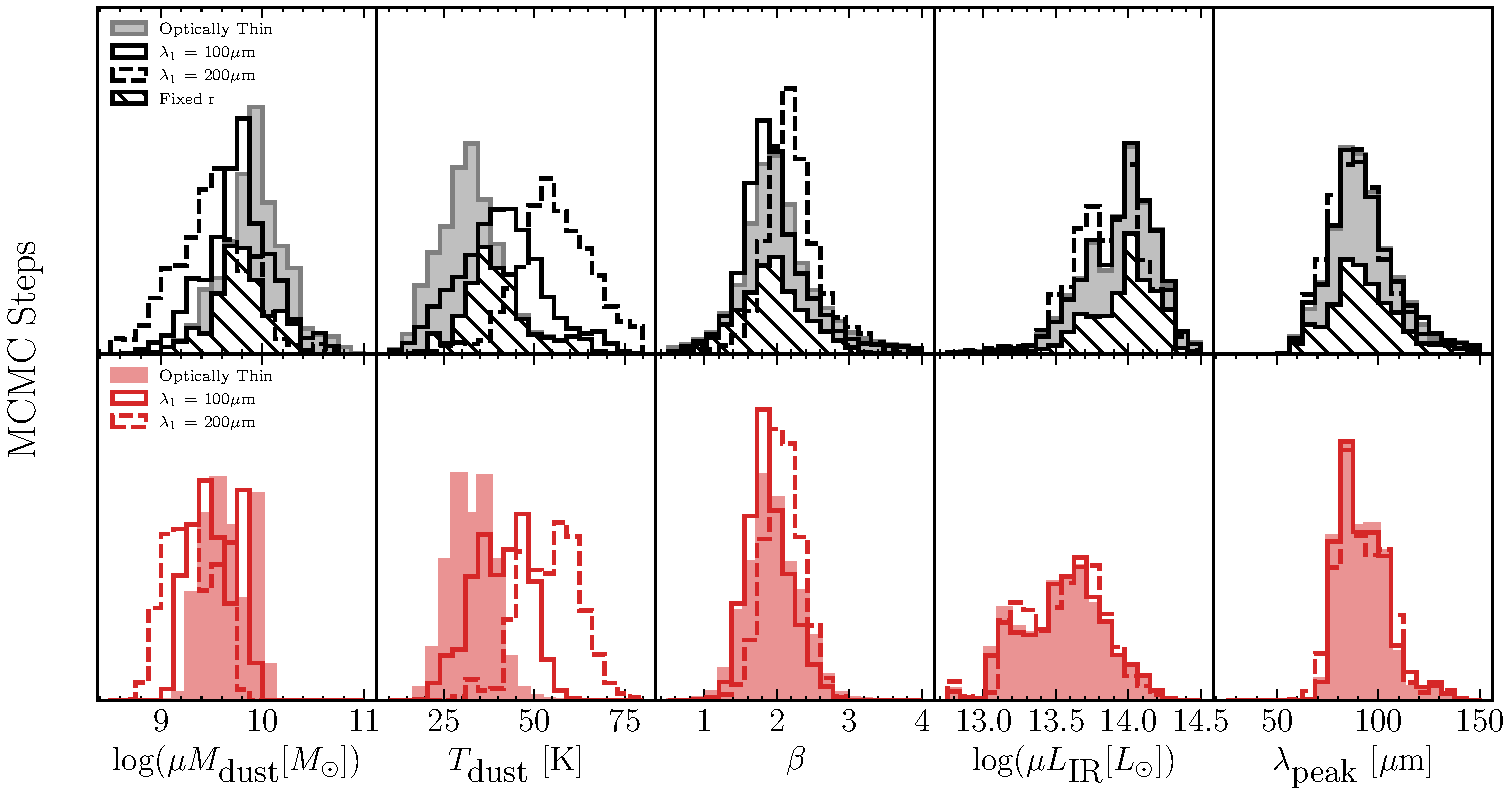
\includegraphics[width=\columnwidth]{Figures/stacked_posterior.pdf}
	\caption[Stacked posterior distributions for each MBB model]{The stacked posterior distributions of log($\mu M_{\textrm{dust}}$), $T_{\textrm{dust}}$, $\beta$, log($\mu L_{\textrm{IR}}$) and $\lambda_{\textrm{peak}}$ for SPT (top panels) and HerBS galaxies (bottom panels). The posterior distribution for each MBB model is illustrated as follows: optically thin (shaded), $\lambda_1 = 100\,\mu$m (solid line), $\lambda_1 = 200\,\mu$m (dashed line) and fixed continuum size (hatched).}
	\label{fig:stacked_posteriors}
\end{figure}

The median values and the $16$th and $84$th percentiles of the probability distributions are listed in Table \ref{tab:parameter_results}. The main parameter of interest, $\beta$, covers only a range of $0.2$ for the three models, showing that it is relatively insensitive to our assumptions about the dust opacity. This conclusion was also found in a recent study of DSFGs selected from the z-GAL NOEMA spectroscopic redshift survey by \citealt{Ismail_2023}. Despite the small range, the model with the highest value of $\lambda_1$, also gives the highest value of $\beta$, a trend that has been observed previously (e.g. \citealt{McKay_2023}). In this study of $870\,\mu$m selected galaxies in GOODS-S, the median $\beta$ systematically increased from $1.78$ and $1.80$ for their optically thin and $\lambda_1 = 100\,\mu$m MBB models, to $2.02$ for $\lambda_1 = 200\,\mu$m. It has recently been suggested that at high redshift a value of $\beta > 2$ might be appropriate for most galaxies (e.g. \citealt{Casey_2019, Casey_2021, Cooper_2022}), but this might suggest that the reason for their anomalous $\beta$ values are their common use of high $\lambda_1$ values. Considering this, future studies concerning the evolution of the dust SED with redshift or comparing DSFGs in the literature, should consider whether $\lambda_1$ is consistent for all sources, and/or should have its own freedom to evolve.

\begin{table}
    \centering
    \begin{tabular}{p{3.5cm}p{2.5cm}p{2.5cm}p{2.5cm}}
	\hline
	\hline
	Parameter & Optically Thin & $\lambda_1 = 100\,\mu$m & $\lambda_1 = 200\,\mu$m \\
	\hline
	\hline
	& \multicolumn{3}{c}{SPT} \\
	\hline
	log($\mu M_{\textrm{dust}} [$M$_\odot]$) & $9.92_{-0.31}^{+0.30}$ & $9.77_{-0.34}^{+0.31}$ & $9.49_{-0.41}^{+0.37}$ \\
	$T_{\textrm{dust}}$ [K] & $32.07_{-8.44}^{+8.43}$ & $40.77_{-11.77}^{+10.90}$ & $55.63_{-9.28}^{+11.20}$ \\
	$\beta$ & $1.98_{-0.39}^{+0.54}$ & $1.91_{-0.32}^{+0.50}$ & $2.18_{-0.30}^{+0.38}$ \\
	log($\mu L_{\textrm{IR}} [$L$_\odot]$) & $13.98_{-0.31}^{+0.19}$ & $13.99_{-0.30}^{+0.19}$ & $13.89_{-0.27}^{+0.23}$ \\
	$\lambda_{\textrm{peak}}$ [$\mu$m] & $90.70_{-12.72}^{+17.33}$ & $90.70_{-13.02}^{+18.36}$ & $89.28_{-13.39}^{+15.21}$ \\
	
	\hline
	& \multicolumn{3}{c}{HerBS} \\
	\hline
	
	log($\mu M_{\textrm{dust}} [$M$_\odot]$) & $9.62_{-0.22}^{+0.30}$ & $9.49_{-0.22}^{+0.31}$ & $9.30_{-0.26}^{+0.33}$ \\
	$T_{\textrm{dust}}$ [K] & $32.73_{-5.92}^{+5.85}$ & $41.16_{-8.20}^{+7.48}$ & $55.18_{-9.23}^{+7.25}$ \\
	$\beta$ & $1.92_{-0.32}^{+0.39}$ & $1.85_{-0.25}^{+0.34}$ & $2.08_{-0.25}^{+0.26}$ \\
	log($\mu L_{\textrm{IR}} [$L$_\odot]$) & $13.55_{-0.37}^{+0.27}$ & $13.57_{-0.37}^{+0.26}$ & $13.57_{-0.34}^{+0.25}$ \\
	$\lambda_{\textrm{peak}}$ [$\mu$m] & $90.03_{-9.28}^{+12.70}$ & $90.36_{-9.46}^{+13.42}$ & $89.96_{-9.46}^{+14.92}$ \\
	\hline
    \end{tabular}
	\caption[Median values of far-IR to mm SED parameters]{The median and 1$\sigma$ errors (estimated from the 16th, 50th and 84th percentiles of the stacked posterior distribution) for the parameters presented in Figure \ref{fig:stacked_posteriors}.}
    \label{tab:parameter_results}
\end{table}

As we observed with SPT0002-52 and HerBS-11, the assumption that the dust is optically thin or thick does have a large effect for dust masses and dust temperatures. There is a clear trend to higher dust temperatures with increasing $\lambda_1$, with differences of approximately $10\,$K and $20\,$K on average between the optically thin and $\lambda_1 = 100\,\mu$m and $\lambda_1 = 200\,\mu$m general opacity models, respectively. Given the inverse correlation between dust mass and dust temperature ($M_\textrm{dust} \propto S_\nu T_\textrm{dust}^{-1}$ for dust masses measured from the Rayleigh-Jeans regime, \citealt{Casey_2014b}), dust masses decrease by approximately $0.1\,$log($\mu M_\odot$) and $0.4\,$log($\mu M_\odot$) from the optically thin model to the $\lambda_1 = 100\,\mu$m and $\lambda_1 = 200\,\mu$m models, respectively. There is no significant difference in the IR luminosities or peak wavelengths between models.

Included in Figure \ref{fig:stacked_posteriors} are the posterior probability distributions for the subset of SPT galaxies where we had estimates for the area of the dust region (hatched histograms). Providing that these galaxies do not represent a biased selection of the total sample, their dust properties are based on a self-consistent dust model that is useful for comparing with the remaining sources. Generally, we find that the distributions for each dust parameter agree best with the optically thin and $\lambda_1 = 100\,\mu$m model, but not always with $\lambda_1 = 200\,\mu$m, suggesting that such a high value may not be appropriate for all SPT detected galaxies. Using the equation relating $\lambda_1$ with the dust surface mass density, $\Sigma_\textrm{dust}$, provided earlier, we find a median value of $\lambda_1 = 88\,\mu$m for these sources, with a $16$th to $84$th percentile range of $44 - 224\,\mu$m. However, this calculation depends heavily on the value assumed for $\kappa_\nu$, which is notoriously uncertain (\citealt{Clark_2016}). The probability distributions for the optically thin model are a good match to those estimated from the subset of galaxies with measured values of $A$, and therefore the parameter estimates quoted herein have been derived using the optically thin model. An added benefit is that the optically thin, isothermal model is widely used in the literature and makes comparisons across studies easier (e.g. \citealt{Magdis_2012, Simpson_2017, Lamperti_2019, Dudzeviciute_2020, Valentino_2020a, daCunha_2021}).

To determine whether the offsets in the assumed model are the same for all galaxies, we show the median values of the parameters estimated from the optically thin model against those estimated from the general opacity models in Figure \ref{fig:comparison_optically_thin_general_opacity}. These panels show the size of the systematic error we might expect if, contrary to our first choice model, the dust is actually optically thick. Here we observe a clear trend in the dust masses and dust temperatures, such that the difference between assuming optically thin and optically thick dust is most extreme for low masses and high temperatures.

\begin{figure}
	\centering
	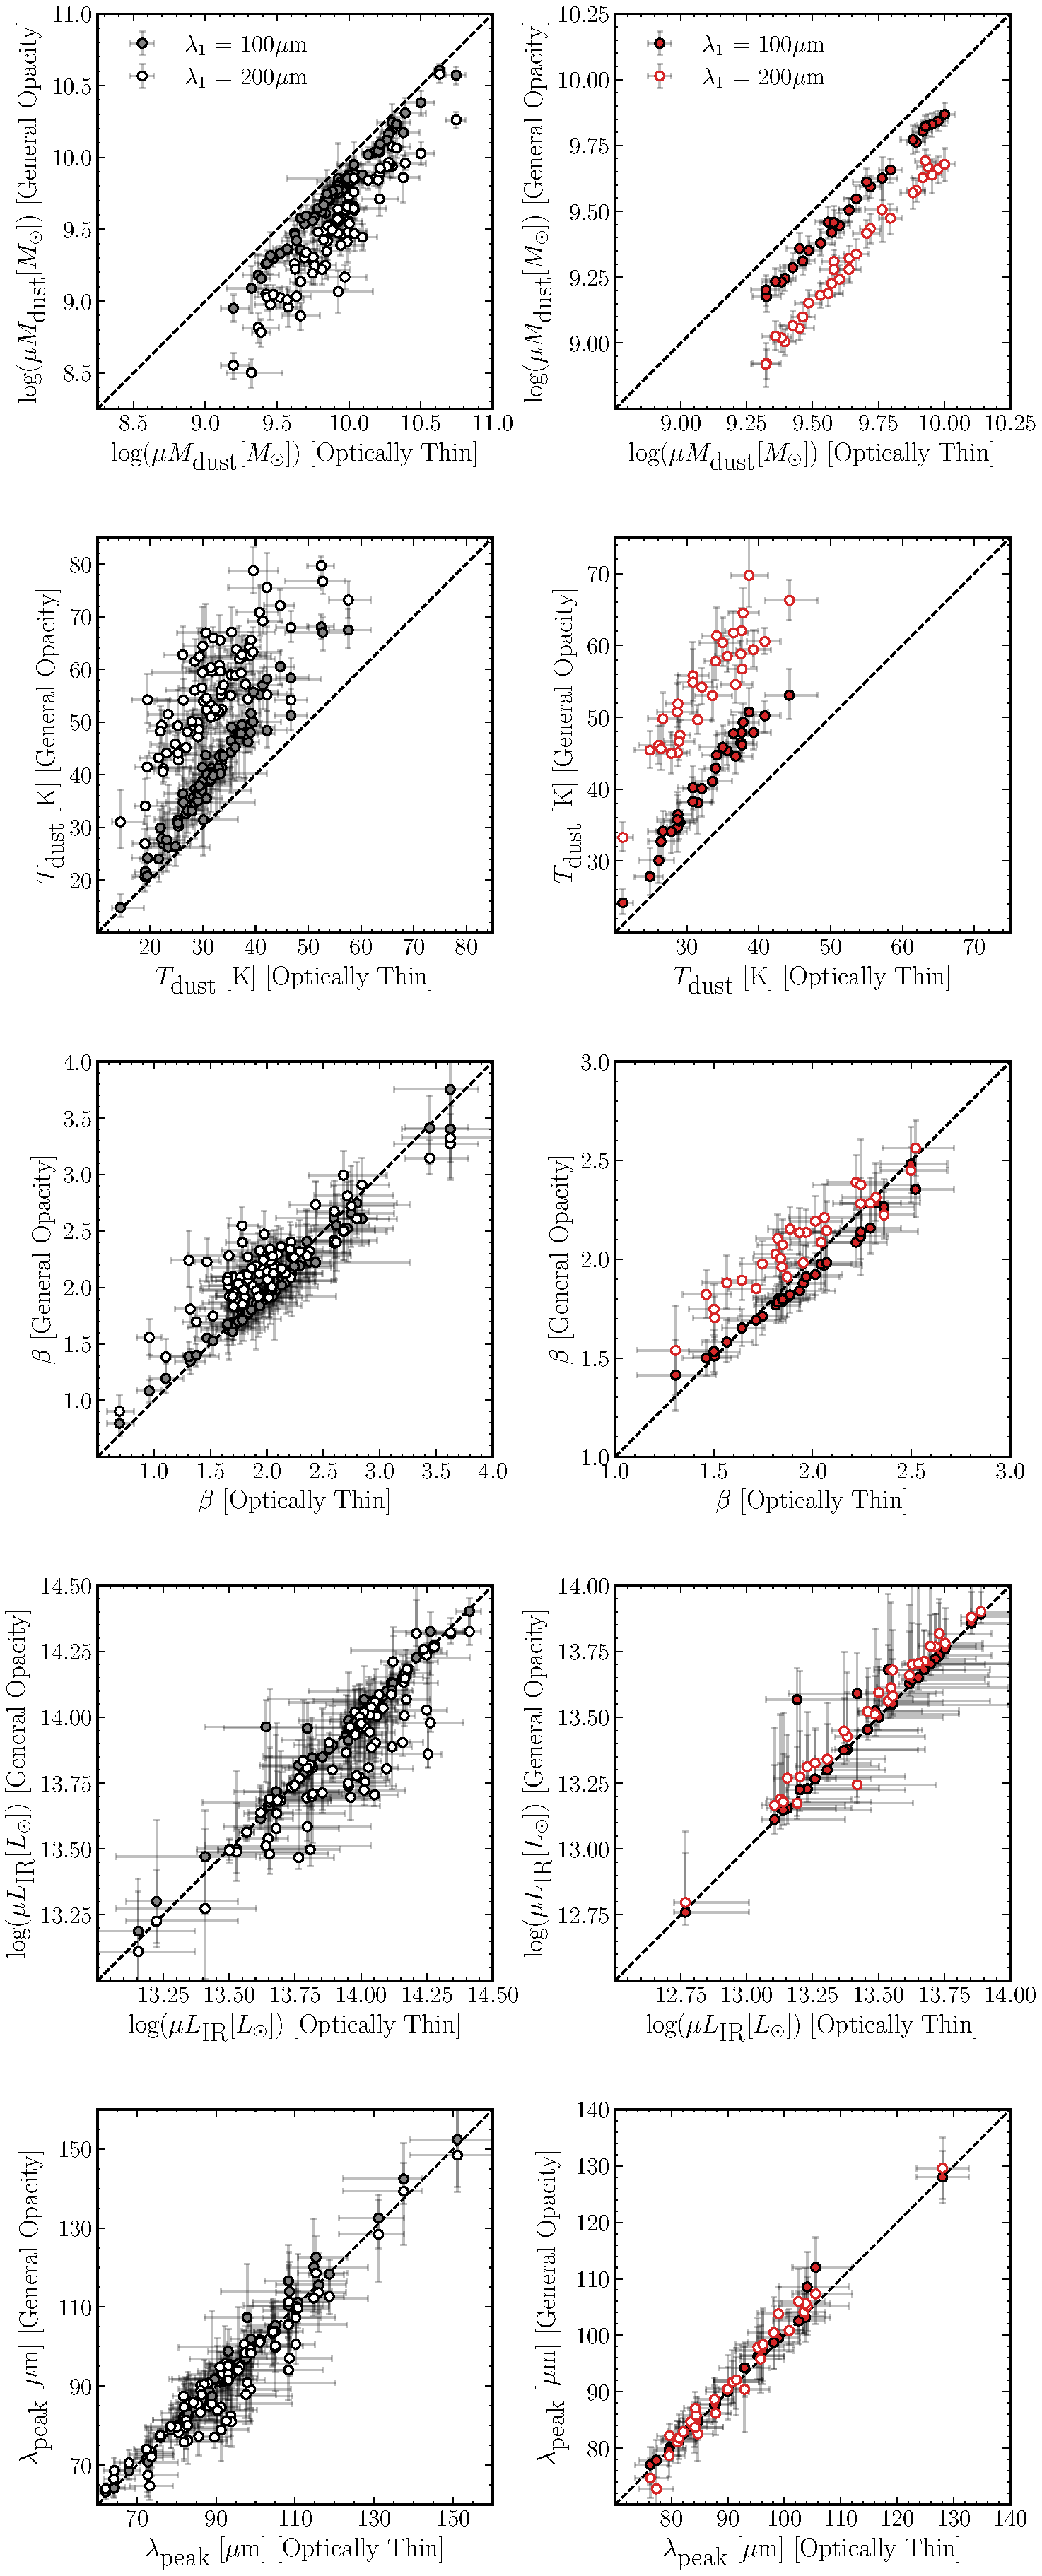
\includegraphics[height=0.9\textheight]{Figures/Figure_4_6.pdf}
	\caption[Comparison of best fitting optically thin and general opacity parameters]{Comparison between the optically thin model and the general opacity models in predicting the dust properties of SPT (left column) and HerBS (right column) galaxies. The general opacity models are shown as filled and open circles for $\lambda_1 = 100\,\mu$m and $200\,\mu$m, respectively.}
	\label{fig:comparison_optically_thin_general_opacity}
\end{figure}

\subsection{The $\beta$-Dust Temperature Degeneracy}

Due to correlated errors between the dust temperature and $\beta$, a well established artificial anti-correlation is observed when fitting. Such a degeneracy between the two parameters has been observed for a wide variety of environments in which an isothermal MBB might be used, ranging in scale from Galactic dust clouds to whole galaxies (e.g. \citealt{Dupac_2003, Desert_2008, Paradis_2010, Schnee_2010, Veneziani_2010, Bracco_2011, Galametz_2012, Paladini_2012, Smith_2012, Lamperti_2019, daCunha_2021}). While many studies report the presence of a correlation between $T_\textrm{dust}$ and $\beta$, it has also been shown that an artificial correlation can be produced from fitting SEDs with large measurement uncertainties (\citealt{Shetty_2009a, Kelly_2012, Juvela_2012a}), and from assuming a constant temperature in scenarios where the reality is that there are multiple dust temperatures along the line of sight to the observer (\citealt{Shetty_2009b, Juvela_2012b}). As a result, it is still debated whether this common correlation represents a true relationship between these properties of the dust, or whether it is artificially produced.

Figure \ref{fig:beta_t_correlation} shows that there is a negative correlation between the measured values of $\beta$ and dust temperature for both sub-samples when assuming the dust is optically thin. The strength of these correlations were tested with the Pearson correlation coefficient, $r_{\textrm{Pearson}}$. The values of $r_{\textrm{Pearson}} = -0.83$ for SPT galaxies and $r_{\textrm{Pearson}} = -0.89$ for HerBS galaxies show that the two sub-samples exhibit a strong negative $\beta$-$T_{\textrm{dust}}$ correlation. In the following section, we address the extent to which the observed $\beta-T_{\textrm{dust}}$ anti-correlation is a true relationship between dust properties, reflecting an intrinsic change in the emissivity properties of dust grains with temperature, and how much is a result of the fitting method. We approach this by comparing our measured dust parameters with those obtained from fitting simulated galaxies. We start on the assumption that there is no correlation between $\beta$ and $T_{\textrm{dust}}$ for our mock galaxies, and then we see if we are able to recover such a relationship from the SED fitting alone.

\begin{figure}
	\centering
	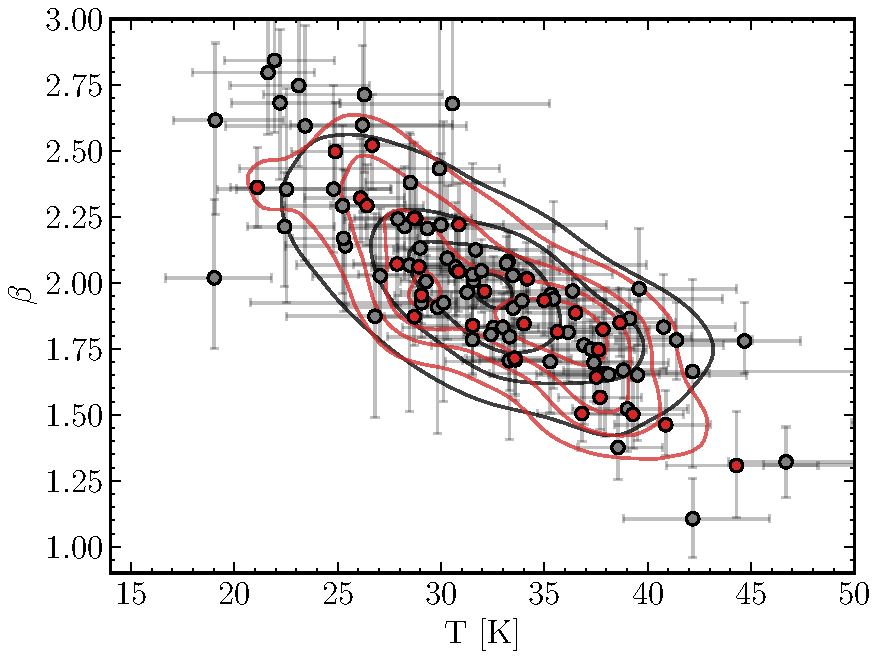
\includegraphics[width=0.8\columnwidth]{Figures/beta_t_correlation.pdf}
	\caption[Relationship between $\beta$ and $T_\textrm{dust}$ for SPT and HerBS galaxies]{Relationship between the dust temperature and the emissivity spectral index for the SPT (black) and HerBS (red) galaxies assuming optically thin dust. The joint posterior distribution for the two sub-samples is shown as contours of the same colour.}
	\label{fig:beta_t_correlation}
\end{figure}

\section{Simulations}
\label{sec:simulations}

In order to assess how accurately our fitting routine derives a galaxy's dust parameters, we ran a suite of mock SEDs with known input parameters and measured how precisely we could recover the dust properties from applying our fitting procedure on our simulated galaxies. We generated our mock galaxies in the following way. First, we assumed that the dust emission can be described by an optically thin, isothermal MBB according to Equation \ref{eq:modified_blackbody_optically_thin}. The need to assume a single model for the dust opacity means that the results of our simulations are only correct under the assumption that the dust in the galaxy is optically thin. As real galaxies are not likely to all be optically thin, ths assumption means that there is an additional uncertainty that would not be accounted for unless the simulations were to be rerun with varying dust opacities. Nonetheless, we continue to produce $2,500$ random SEDs by selecting dust parameters randomly between the lower and upper bounds defined in Table \ref{tab:simulation_inputs}. These values were selected specifically to recreate the width of the posterior distributions observed for real sources. We generated two sets of mock galaxies, one to represent SEDs similar to the real SPT galaxies, and one set that simulates real HerBS galaxies. For the mock HerBS sources we placed each galaxy at a random redshift between $2$ and $4$ and obtained from it flux densities at the same observed wavelengths as for the real HerBS sub-sample (recall Section \ref{sec:sed_fitting}), omitting photometry at $1.2\,$mm as only a few HerBS sources have photometry at this wavelength. In a similar manner, the second sample of mock SPT galaxies were placed at a random redshift between $2$ and $6$, and given the same photometric coverage as a typical SPT galaxy. These $5,000$ SEDs are currently models with known inputs; to create observed SEDs, we add flux errors to the models, drawing randomly from a Gaussian distribution with a standard deviation derived from the spread in SNR of real sources at that wavelength. We also assumed a lensing magnification of $5.5$ for SPT galaxies and $5.3$ for HerBS galaxies, in keeping with their median values.

\begin{table}
    \centering
    \begin{tabular}{p{3cm}|p{3cm}}
        \hline
		\hline
        Parameter & Bounds \\
        \hline
        \hline
        log($\mu L_{\textrm{IR}} [L_{\odot}]$) & 13 -- 14 (HerBS) \\
        & 13 -- 14.5 (SPT) \\
		$T_{\textrm{dust}}$ [K] & 20 -- 50 \\
		$\beta$  & 0.5 -- 4 \\
		$\alpha$  & 1 -- 5 \\
        \hline
    \end{tabular}
    \caption[Bounds on the input parameter ranges for mock galaxy simulations]{The upper and lower bounds assumed on the flat priors during the input-output simulations described in Section \ref{sec:simulations}.}
    \label{tab:simulation_inputs}
\end{table}

We added calibration errors in the same manner that we do for the real DSFGs and derived the dust parameters using the same modelling procedure detailed earlier. When fitting we test to see whether the mock galaxy would be detected in our sub-samples (assuming detection limits of $80\,$mJy at $500\,\mu$m for HerBS and $25\,$mJy at $870\,\mu$m for SPT) and remove mock galaxies if they fail to meet the detection limits.

In Figure \ref{fig:in_out_simulations} we show the measured dust properties of the two artificial samples, plotted against their input values. We show the input and output dust masses, dust temperatures and $\beta$ values, all of which are in good agreement, a reflection of the excellent coverage spanning both the thermal peak of dust emission and the Rayleigh - Jeans tail. The root mean square error (RMSE) is calculated for each dust parameter, illustrating the intrinsic scatter that real galaxies have around their optically thin dust parameter inputs, which we have assumed to be their true values. From these values, we know that our real DSFGs recover their true dust masses to $0.05\,$dex and $0.03\,$dex, dust temperatures to $1.63\,$K and $1.61\,$K and $\beta$ to $0.13$ and $0.09$ for SPT and HerBS galaxies, respectively. The accuracy of the output dust temperatures decreases for warmer temperatures, a result of the SED shifting to shorter wavelengths and the peak being less constrained by the \textit{Herschel} photometry. The right-most panel of the two rows in Figure \ref{fig:in_out_simulations} show the difference in the input and output dust temperatures against the difference in the input and output $\beta$ values. As the mock galaxies are initialized with no intrinsic correlation, the anti-correlation observed here must have been introduced by correlated errors in the two parameters. We measure the RMSE in $\beta$ and $T_\textrm{dust}$ to be approximately $0.1$ and $1.6\,$K, respectively. The RMSE in the $\beta$ and $T_\textrm{dust}$ measurements for real sources (Figure \ref{fig:beta_t_correlation}) are $0.5$ and $8\,$K, respectively. This suggests that the fitting of mock galaxies with no intrinsic correlation does not produce an artificial anti-correlation that can account for the typical RMSE of real galaxies, and thus there is a genuine inverse correlation (of some lesser degree than actually observed in Figure \ref{fig:beta_t_correlation}) between $\beta$ and $T_\textrm{dust}$ that is not caused by correlated measurement errors. However, it is difficult to predict the extent to which the scatter in this relationship is a result of the dust opacity model. It is likely that the RMSE for mock galaxies would be larger if they were free to have a wider selection of dust opacities, and as a result, this conclusion is only valid in the case where all galaxies are assumed to be optically thin.

\begin{figure}
	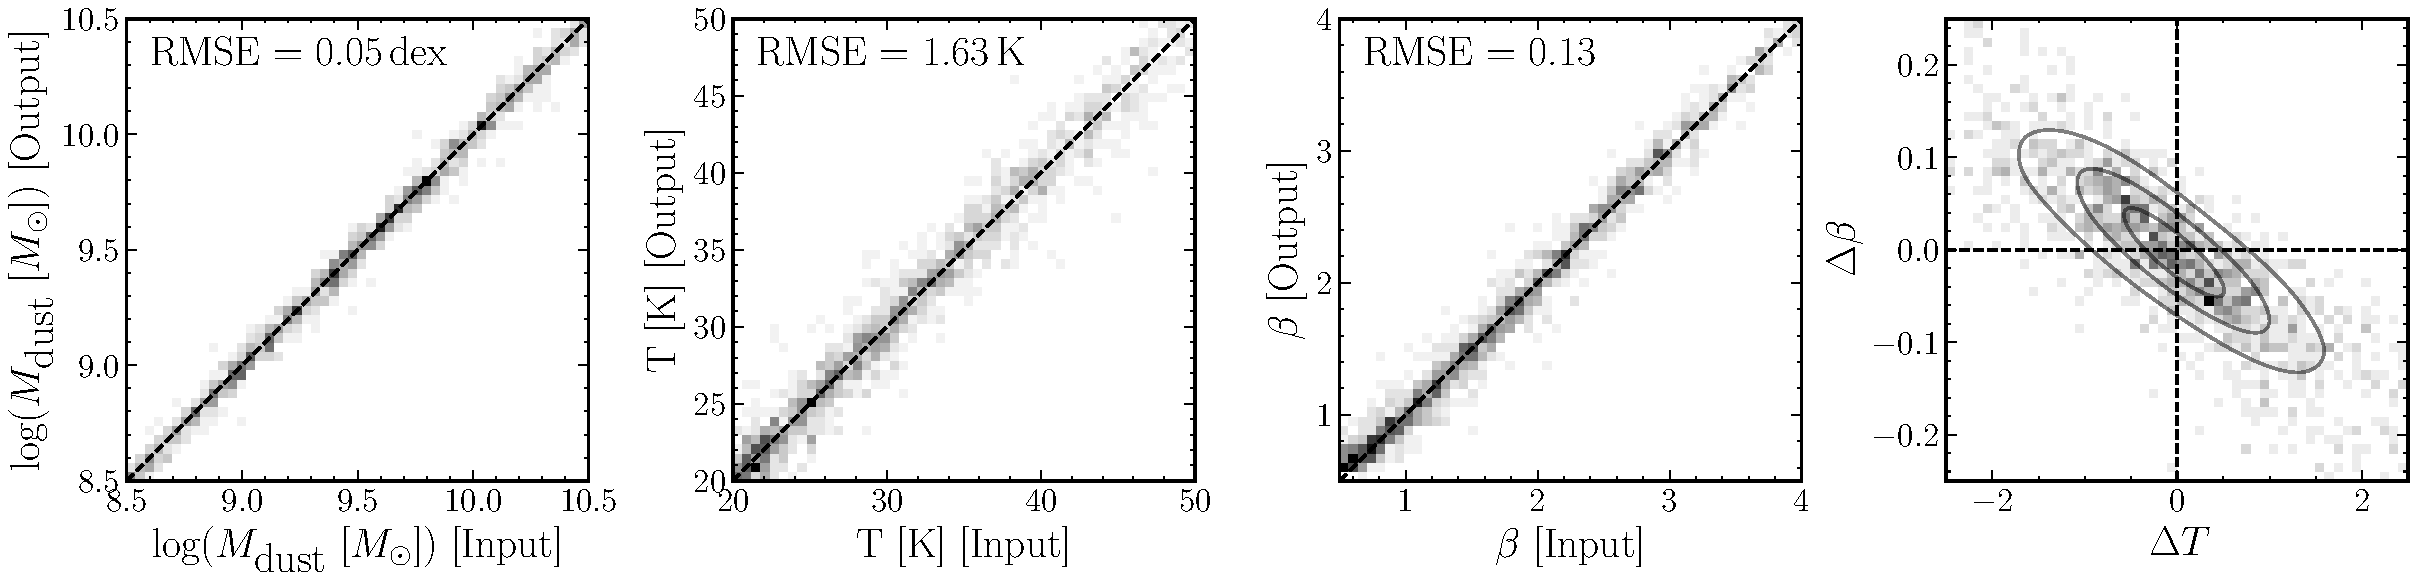
\includegraphics[width=\columnwidth]{Figures/Figure_4_8_part1.pdf}
	\centering
	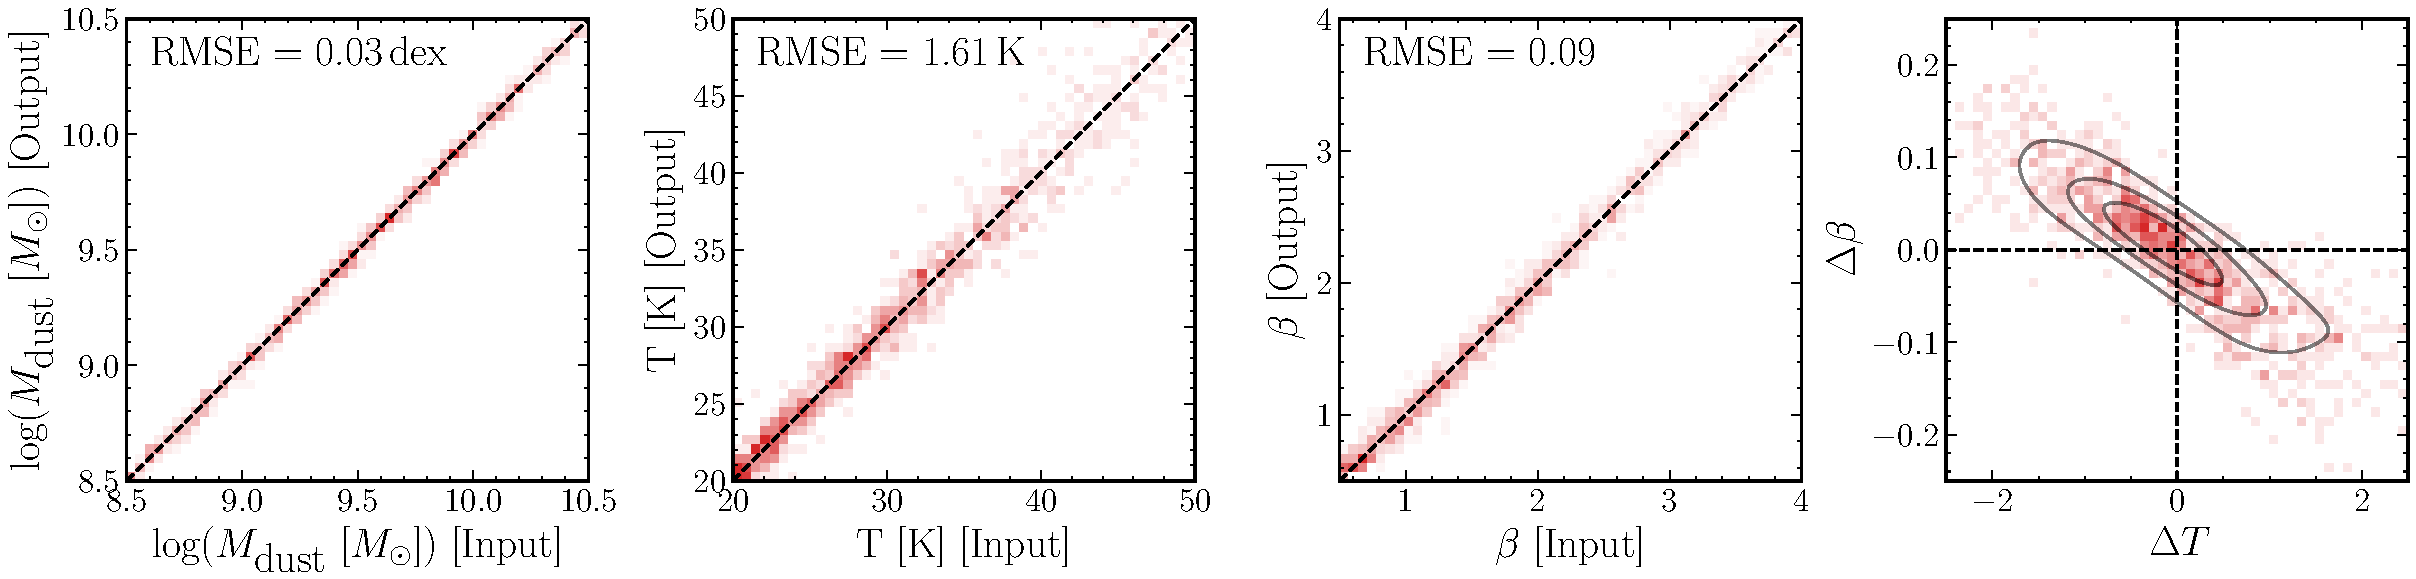
\includegraphics[width=\columnwidth]{Figures/Figure_4_8_part2.pdf}
	\caption[Comparison of the input and output parameter values from simulations]{The input values compared to the measured output values for the simulations described in Section \ref{sec:simulations}. The panels show the following dust parameters: dust mass, dust temperature and dust emissivity index, and the difference between the inputs and outputs in the dust temperature - $\beta$ plane. The top row (black) shows the results of the simulation of SPT galaxies with optically thin dust, while the bottom row (red) represents mock HerBS galaxies.}
	\label{fig:in_out_simulations}
\end{figure}

\section{Evolution of Dust Properties with Redshift}
\label{sec:redshift_evolution}

In this section, we study the redshift evolution of the measured dust properties of HerBS and SPT galaxies in context with low redshift predictions from the Milky Way and local star forming galaxies.

\subsection{Evolution of $\beta$ with Redshift}

Figure \ref{fig:beta_z_evolution} shows the distribution of galaxies in the $\beta-z$ plane. The average value of the dust emissivity spectral index, as measured from the median of each galaxy's posterior distribution in $\beta$, is $1.98$ for SPT and $1.91$ for HerBS galaxies. These values are higher than the values typically assumed in the local Universe. For example, it is significantly higher than the value in our Galaxy, which is uniformly $\beta = 1.51\pm0.01$ across the sky (\citealt{Planck_Collaboration_2015}), and is at the upper end of the range observed for nearby galaxies in JINGLE ($\beta = 0.6 - 2.2$, \citealt{Lamperti_2019}). It is interesting to note, however, that the higher values observed in JINGLE are measured for the most massive galaxies in the sample, which could be the descendants of the DSFGs studied here (\citealt{Eales_2023}, see also Chapter \ref{chapter:Radio_Identifications}). It is difficult to reconcile the $\beta$ values measured for the DSFGs studied here with the values locally, and with the increasing number of recent studies that suggest high redshift galaxies may be better described by an SED with $\beta \sim 2$ (e.g. \citealt{daCunha_2021, Witstok_2023}), we also advocate that future studies of high redshift galaxies adopt this value.

\begin{figure}
	\centering
	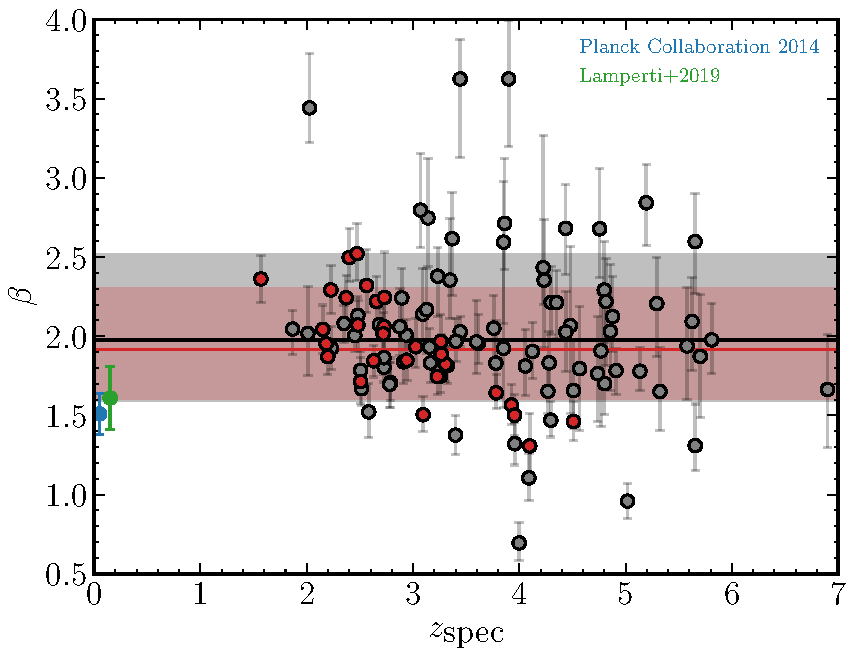
\includegraphics[width=0.76\columnwidth]{Figures/beta_evolution.pdf}
	\caption[Distribution of HerBS and SPT galaxies in the $\beta$ - redshift plane]{The distribution of $\beta$ values for HerBS (red) and SPT (black) galaxies against redshift with the canonical values from the JINGLE survey (green) and the Milky Way (blue). The median value of the stacked posterior distributions are shown as red and black lines for the HerBS and SPT samples respectively, with the shaded regions showing the $16$th to $84$th percentiles.}
	\label{fig:beta_z_evolution}
\end{figure}

Considering the two sub-samples collectively, there is little evidence to suggest that there has been any evolution in $\beta$ over the redshift range $2 < z < 6$. There appears a decreasing trend of $\beta$ with cosmological distance for HerBS galaxies, but this is mostly influenced by the five sources observed at $z \sim 4$. The $500\,\mu$m selection wavelength at $z \sim 4$ is close to the peak in the dust emission, thus biasing us to higher dust temperatures. Given the anti-correlation with $\beta$, it may not be surprising that we observe lower $\beta$ at this redshift for HerBS galaxies. The lack of a redshift evolution in $\beta$ has also been observed in previous studies including \citealt{Ismail_2023} ($2 < z < 3$) and \citealt{Witstok_2023} - a study of $17$ galaxies across $4 < z < 8$.

\subsection{Variation in $\beta$}

While there appears to be no evolution of $\beta$ with redshift, we still observe significant scatter around the average values, which tells us that either measurement errors are scattering values around some common $\beta$, or there is true diversity in the physical and chemical properties of high redshift galaxies. To assess which of these are true, we repeated the simulations from the previous section, except this time we randomly draw $\beta$ from a uniform distribution between $1\sigma$ above and below the average observed value. This aims to replicate a single population of galaxies with a common $\beta$ value which, if they scatter to a significantly wide distribution after fitting, tells us that the cause is likely measurement errors. The simulations are run in the same way as before, except we now have a narrower range of input beta values ($1.68 - 2.41$ for SPT and $1.61 - 2.26$ for HerBS) and we explore all redshifts between $z = 0$ and $z = 7$.

Figure \ref{fig:beta_z_simulation} shows the difference between the input and output $\beta$ values of these simulations ($1,000$ for each sub-sample), as a function of the input redshift. We find no reason to believe that our fitting procedure underestimates or overestimates the value of $\beta$ at any redshift. For the highest redshift SPT galaxies, the scatter around the \textit{true} $\beta$ appears larger than at $z \sim 0$. However, assuming that the RMSE is approximately equal at all redshifts (which appears to be the case in at least the HerBS galaxies), then we estimate the RMSE on $\Delta \beta$ is $\sim 0.1$ for both sub-samples. The scatter in our measured $\beta$ values in Figure \ref{fig:beta_z_evolution} is $\sim 0.3 - 0.5$, which shows that the measurements errors are smaller than the observed scatter. This implies that the range of $\beta$ observed in Figure \ref{fig:beta_z_evolution} represents a true diversity in the dust properties of DSFGs (providing that optically thin mock galaxies are a suitable representation of the two samples). The range of $\beta$ that we measure in this study is also not unusually high for high redshift galaxies as the spread in $\beta$ is corroborated by studies such as \citealt{daCunha_2021}, \citealt{Cooper_2022}, \citealt{Ismail_2023} and \citealt{Witstok_2023}.

\begin{figure}
	\centering
	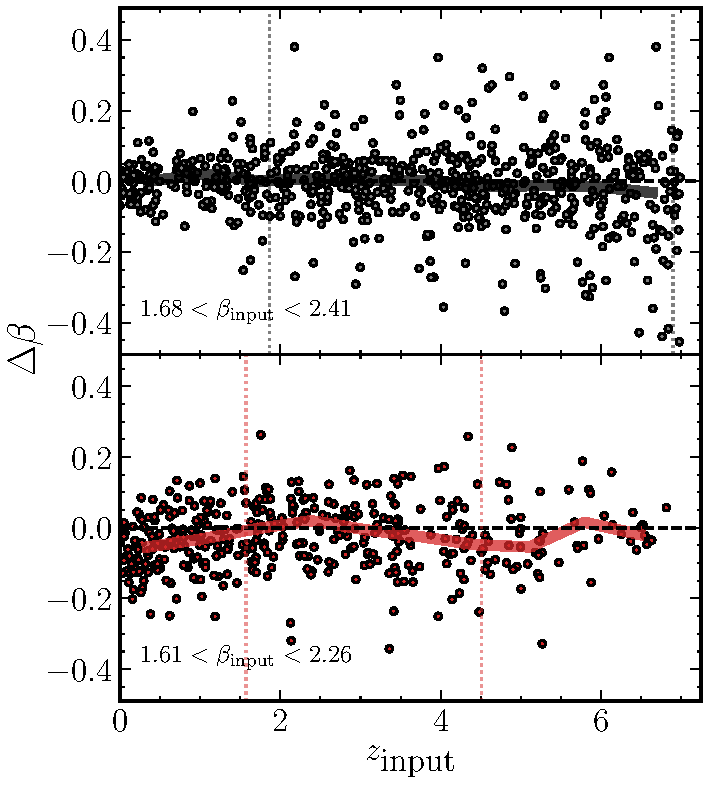
\includegraphics[width=0.74\columnwidth]{figures/beta_simulations.pdf}
	\caption[Difference between input and output $\beta$ from simulations of mock galaxies]{The difference between the input and output $\beta$ values, $\Delta \beta = \beta_{\textrm{output}} - \beta_{\textrm{input}}$, as a function of the input redshift for mock SPT galaxies (top panel) and mock \textit{Herschel} galaxies (bottom panel). Dotted vertical lines represent the minimum and maximum redshift observed in each sample and the thick solid lines represents the median in $\Delta \beta$ as a function of redshift}
	\label{fig:beta_z_simulation}
\end{figure}

A few SPT galaxies have anomalously high $\beta$ ($\gtrsim 2.5$). We mentioned earlier that high values of $\beta$ could arise from the patchwork nature of far-IR to mm SEDs, where we combine single-dish observations with interferometric observations from ALMA. To see if the increased spatial resolution of ALMA has split the low resolution sources into multiple components, some of which may subsequently be lost below the ALMA detection threshold at $3\,$mm, we refit a selection of SPT galaxies with high $\beta$ values, removing the ALMA $3\,$mm photometry and assuming $\beta = 2$. These sources are: SPT0112-55 ($\beta = 3.62$), SPT0611-55 ($\beta = 3.44$), SPT2335-53 ($\beta = 2.68$), SPT2340-59 ($\beta = 2.71$) and SPT2349-52 ($\beta = 3.62$). When we then compare the observed $3\,$mm flux density with the predicted value from the $\beta = 2$ MBB, we find that the observed $3\,$mm flux density would need to be $60 - 80\%$ lower than the true flux density to explain such high $\beta$ values. Despite the blending of high redshift galaxies observed in \textit{Herschel} beams (see Chapter \ref{chapter:Radio_Identifications}), this seems unlikely, and the high $\beta$ sources may be genuine. A common explanation for the steepening of the Rayleigh-Jeans tail in high redshift galaxies is CMB heating, which causes a greater reduction in the flux density at the longest wavelengths (\citealt{daCunha_2013}). However, this is accounted for in our SED modelling (Equations \ref{eq:modified_blackbody_general_opacity_a_cmb} and \ref{eq:modified_blackbody_optically_thin}) and does not have a large impact on the shape of the SED except for galaxies at $z \gtrsim 5$ at low dust temperatures. Other properties that affect the measurement of $\beta$, such as the geometry of the ISM and distributions in dust temperature, would likely act to flatten the Rayleigh-Jeans tail (as can be visualized from the coadding of SEDs at different temperatures). The higher $\beta$ of these sources could potentially represent a difference in the composition of their interstellar dust, with $\beta > 2$ being associated with amorphous silicates (e.g. \citealt{Draine_1984, Agladze_1996, Meny_2007}).

\subsection{Evolution of $T_{\textrm{dust}}$ with Redshift}
\label{sec:dust_temperature_evolution}

Whether the dust temperature of DSFGs evolves with redshift is a matter of contention in the literature, with studies often claiming completely opposing views. Advocating for hotter dust temperatures at high redshift (e.g. \citealt{Magdis_2012, Magnelli_2014, Swinbank_2014, Bethermin_2015, Faisst_2017, Schreiber_2018, Zavala_2018b, Liang_2019, Ma_2019, Faisst_2020, Bakx_2021, Witstok_2023}), such observational studies are corroborated by the idea that at higher redshifts specific star formation rates (sSFR) and lower dust abundances would lead to hotter dust temperatures. An important caveat to these works is that dust temperature correlates with luminosity (\citealt{Dunne_2000}), which if not adequately accounted for, would naturally lead to a relationship between temperature and redshift. While some studies report a fall in dust temperature (e.g. \citealt{Symeonidis_2013}), most others report little or no evolution (e.g. \citealt{Casey_2018, Jin_2019, Lim_2020a, Dudzeviciute_2020, Reuter_2020, Barger_2022, Drew_2022, Witstok_2023}).

As we showed earlier, the luminosity-weighted dust temperature obtained from SED fitting is dependent on the assumptions we make about the opcaity of the dust. However, the wavelength where the thermal dust emission peaks, $\lambda_\textrm{peak}$, is insensitive to the choice we make, and from Wien's displacement law, we can derive a characteristic dust temperature that we shall name $T_\textrm{peak}$. Neither dust temperature will be the same as the true temperature of the dust in the ISM, but $T_\textrm{peak}$ does allow us to study the evolution in temperature with redshift. 

The top panel of Figure \ref{fig:t_evolution} shows the distribution of SPT and HerBS galaxies in the IR luminosity - redshift plane, along with the detection limits for the two sub-samples assuming a dust temperature of $32\,$K (the median dust temperature of the combined sample) and $\beta = 2$. To avoid any selection effect from the aforementioned luminosity-temperature relationship, we define a small range of IR luminosity for both samples that stays clear of the detection limit (dashed boxes). In the bottom panel of the same figure, we then plot the temperature, as derived from Wien's law, as a function of redshift for the sources in the boxed regions. We compare our measurements of the peak dust temperature ($T_{\textrm{peak}} = 2.898 \times 10^3$ [$\mu$m K]/$\lambda_{\textrm{peak}}$ [$\mu$m]) with the observational relationships derived in the studies of \citealt{Schreiber_2018}, \citealt{Bouwens_2020} and \citealt{Viero_2022}, as well as the median dust temperature of the JINGLE survey. For the combined SPT and HerBS sample there appears little evidence for evolution of temperature with redshift, with peak dust temperatures between $2 < z < 6$ similar to those at $z = 0$ from the observational trends.

\begin{figure}
	\centering
	\includegraphics[width=0.8\columnwidth]{Figures/t_evolution.pdf}
	\caption[Distribution of HerBS and SPT galaxies in the $L_{IR} - z$ and $T_\textrm{peak}-z$ planes]{Top panel: the distribution of HerBS (red) and SPT (black) galaxies in the $\mu L_{\textrm{IR}}-z$ plane. The red and black lines represent the detection limit of a HerBS source detected at $> 80\,$mJy ($500\,\mu$m) and an SPT source detected at $> 25\,$mJy ($870\,\mu$m), assuming a dust temperature of $32\,$K and $\beta = 2$. The boxed regions show the limits of our luminosity-limited set of sources from which we test evolutionary trends in the dust temperature. Bottom panel: The distribution of peak dust temperature with redshift for the sources selected in our luminosity-limited subsets. Observed trends from \citealt{Schreiber_2018}, \citealt{Bouwens_2020} and \citealt{Viero_2022} are illustrated as blue, orange and purple lines, respectively. The median dust temperature of local sources from the JINGLE survey is shown as the green error bar.}
	\label{fig:t_evolution}
\end{figure}

\section{Conclusions}

In the previous Chapter we introduced various studies that measure the dust mass density out to high redshifts. This is but one example where our interpretation of galaxy evolution is dependent on the simple assumption that the interstellar dust is the same at all times (specifically that it takes the physical and chemical form of the dust we can observe in the Galaxy and in local galaxies). In this Chapter, we challenged this assumption. We selected roughly $100$ galaxies from HerBS and the SPT-SZ surveys based on photometric coverage at observed wavelengths $>1\,$mm, allowing us to measure well constrained $\beta$ values (as well as ensuring sufficient coverage of the thermal peak in order to constrain the temperature and mass of the dust grains). We modelled the far-IR to millimeter spectra of these galaxies with three models: an optically thin MBB; a general opacity model (which allows for optically thick dust) where the transition between thick and thin is set at $100\,\mu$m; and a third with the transition at $200\,\mu$m. We systematically measured lower masses and higher dust temperatures for the general opacity models but observed no change in the IR luminosities or dust emissivity index. We identified a strong correlation between $\beta$ and dust temperature, which could not be accounted for by the degeneracy between the parameters when fitting the SEDs, suggesting a genuine anti-correlation. We obtained an average value of $\beta = 1.96$, which is higher than in the Galaxy and at the high end of the range observed for local galaxies in JINGLE, although no correlation was observed with redshifts between $z = 2$ and $z = 6$. We advocate for a higher value of $\beta \sim 2$ in future extragalactic studies, as opposed to nominal values between $1.5$ and $1.8$. Finally, we selected a subset of galaxies with similar luminosities from both sub-samples and found that there appears to be no strong evolution in their dust temperatures with redshift.


\chapter{Radio Observations of \textit{Herschel} Galaxies}
\label{chapter:Radio_Identifications}
\sloppy

\section{Introduction}

For samples of star forming galaxies in the local and high redshift Universe there is a well observed correlation between the far-infrared and radio emission (e.g. \citealt{Dickey_1984, deJong_1985, Helou_1985, Condon_1992, Barger_2000, Yun_2001, Garrett_2002, Appleton_2004, Ibar_2008, Seymour_2009, Sargent_2010}), that remains nearly linear over multiple orders of magnitude in far-infrared luminosity ($10^{9} \lesssim L_{\textrm{FIR}} [L_{\odot}] \lesssim 10^{12.5}$). The small scatter in this relation is often attributed to the \textit{calorimeter model} (\citealt{Voelk_1989, Lisenfeld_1996, Lacki_2010}), which ascribes the far-infrared and radio emission to common stellar sources. In this model, galaxies are opaque to UV light from massive OB-like stars which gets absorbed by the dust in the ISM and reradiated in the far-infrared. Observations in the far-infrared and sub-mm are thus sensitive to the cold dust that reradiates the energy from young stars. These stars quickly come to the end of their lives, exploding as Type II supernovae, producing cosmic ray electrons and positrons. These cosmic rays are emitted with relativistic velocities that radiate energy in the radio as synchrotron radiation when spiralling around galactic magnetic fields. The concurrence of the far-IR and radio emission in a galaxy means that the radio continuum is a useful tracer of recent, obscured star formation.

The prevalence of a correlation at such a wide span of redshifts and luminosities has lead to studies that use the radio emission as an unbiased tracer of obscured star formation in dusty galaxies across time (\citealt{Kennicutt_2012}). By making use of the tight far-IR/radio correlation (FIRC), as well as the benefits we shall outline in the following section, we can identify counterparts to low resolution sources with greater confidence than we would expect if we directly matched to the optical or near-infrared, which allows for better characterization of the galaxies' properties. In this Chapter, we identify $3\,$GHz VLA counterparts to \textit{Herschel} detected galaxies in the $\sim2\,$deg$^2$ COSMOS field. The radio galaxies themselves have short wavelength counterparts provided by the COSMOS2020 catalogue, that we match unambiguously due to their much smaller positional errors.

\section{Identifying Multiwavelength Counterparts to DSFGs via the Radio}

As illustrated in Chapter \ref{chapter:Data_Release_3}, DSFGs that are detected with single dish far-IR/sub-mm telescopes with low angular resolution will likely include multiple galaxies in the optical or near-infrared within the beam width. This is a particular problem for \textit{Herschel} where even the smallest SPIRE beam size, at $250\,\mu$m, has a FWHM of $\sim 18\,$arcsec, making the decision as to the source of the far-IR emission difficult. This is further compounded by the intrinsic faintness of optical counterparts due to dust obscuration. In the following sections we detail a method for identifying radio counterparts to \textit{Herschel} sources, that makes use of the FIRC to identify them with high confidence. This circumvents the uncertainty that comes from statistical methods that match directly to short wavelength counterparts by first matching them with radio sources that have small positional errors, thus generating a clean and more complete sample. The following is a list of benefits of using the radio emission for this purpose:

\begin{enumerate}
    \item Star forming galaxies are known to produce a lot of synchrotron emission. This allows us to take advantage of the FIRC to locate the galaxy emitting the radiation in the far-IR. Unlike optical counterpart searches, radio IDs are not solely motivated by their position and brightness, but also by the fact that the two regimes are linked to a common source.
    \item Even when considering the deepest radio maps, the low surface density of radio sources means that the probability of a chance positional alignment is unlikely. As a result, we can have a reasonable confidence in there being some association between objects when we do observe radio sources in close proximity to the far-IR/sub-mm position (\citealt{Ivison_2002, Borys_2004}). In most cases (as we shall validate in this study), radio sources are sufficiently rare that finding an object within the positional uncertainty of the far-IR/sub-mm beam almost always results in a robust identification.
    \item When a secure radio counterpart is identified, the positional accuracy ($\sim 1\,$arcsec for the Karl G. Jansky Very Large Array (VLA) at $1.4\,$GHz and $\sim 0.75\,$arcsec at $3\,$GHz) allows for an unambiguous identification with an optical or infrared galaxy counterpart. By first locating these galaxies via their radio identification, we predict a low false identification rate which gives us greater confidence in characterizing their colours, morphologies, stellar masses and more.
\end{enumerate}

While the radio emission from star forming galaxies allows for more secure identification of counterparts across the electromagnetic spectrum, it also has several drawbacks. The following is a list of disadvantages to using radio emission for this purpose:

\begin{enumerate}
    \item Our understanding of the radio-selected DSFG population is likely to be skewed by selection effects. The negative K-correction in the far-infrared arises due to the steep Rayleigh-Jeans part of the SED and allows for nearly equal detection of dusty galaxies at $z \sim 0.5$ as $z \sim 8$ (\citealt{Blain_2002}). The radio, however, suffers from a strong positive K-correction which causes a bias against high redshift galaxies ($z > 3$). This means that a substantial fraction of far-IR and sub-mm detected galaxies remain undetected in the radio due to the lack of sufficiently deep radio data.
    \item Long wavelength interferometry has been used to show that for far-IR/sub-mm sources in which we observe multiple radio galaxies in close proximity, in $\sim 80\%$ of cases the thermal dust emission is associated from only one of the radio sources. This leads to an ambiguity as to the nature of some apparent multiple systems. This will be discussed in more detail in Section \ref{sec:multiple_systems}.
    \item Potentially the most important drawback for the identification of far-IR/sub-mm emitting galaxies, is the sky coverage from radio surveys. While we have large sky surveys in the far-IR such as \textit{Herschel}-ATLAS, using deep radio data for such large area surveys is not yet practical. Future radio surveys such as the Square Kilometre Array (SKA) and recent wide-area surveys with the Low-Frequency Array (LOFAR) will allow us to produce larger samples of DSFGs.
\end{enumerate}

Many studies have found success in adopting a frequentist approach to searching for possible radio counterparts to far-IR and sub-mm sources (e.g. \citealt{Eales_2009, Dye_2009, Dunlop_2010} and references therein). This typically involves using Monte Carlo simulations to estimate the probability that a given radio source is located near the far-IR/sub-mm position by chance. This is a reversed view of counterpart crossmatching compared to the Likelihood Ratio method described in Chapter \ref{chapter:Data_Release_3}. In the LR technique we defined a probability of association for each possible counterpart, whereas here, with the lower surface density of radio objects on the sky, a better question to ask ourselves is: how many ways would we expect to observe a given candidate by chance? This naturally lends itself to using a Monte Carlo approach. The advantage of using such a frequentist approach over a Bayesian method is that it does not require assumptions to be made about the form of the far-IR/sub-mm positional errors, given that they are poorly known due to source confusion.

\section{Identifying Radio IDs to \textit{Herschel} Sources in COSMOS}

In the following sections we identify radio counterparts to \textit{Herschel} detected sources in the Cosmic Evolution Survey (COSMOS). We applied the frequentist method of \citealt{Lilly_1999}, which differs from the Bayesian Likelihood Ratio method in that it searches for objects close to the far-IR source and estimates the probability that each object is a chance alignment, rather than estimating the probability the two are physically associated.

COSMOS is a deep, wide area survey of an equatorial two square degree field centered at R.A $+150.12^{\circ}$ and declination $+2.21^{\circ}$ (\citealt{Scoville_2007}). The field has been observed with many space-based (e.g. \textit{Hubble Space Telescope}, \textit{Spitzer}, \textit{Chandra} and \textit{Herschel}) and ground-based telescopes (e.g. Keck, VLA and UKIRT), resulting in multiwavelength data that spans from the X-ray to radio wavelengths. The high sensitivity and resolution of these data sets over a sufficiently large area, allows for comprehensive studies on the co-evolution of galaxies (\citealt{Schreiber_2018}; \citealt{Stockmann_2020}; \citealt{Valentino_2020a}), star formation (\citealt{Gruppioni_2013}; \citealt{Novak_2017}), large scale structure (\citealt{Scoville_2013}; \citealt{Laigle_2018}) and AGN (\citealt{Prescott_2006}; \citealt{Heintz_2016}). 

\subsection{\textit{Herschel} Observations in COMSOS}

The \textit{Herschel} detected sources that we study in this work were taken as part of the \textit{Herschel} Multi-tiered Extragalactic Survey (HerMES; \citealt{Oliver_2012}). HerMES is a deep far-infrared imaging survey of some of the most well-studied blank extragalactic fields. The survey design of HerMES allowed for the detection of a wide range in far-IR luminosities by targeting high luminosity objects which are bright but rare in wide, shallow surveys and the lower luminosity objects, which are faint but common, in deep, narrow surveys. As such, fields range in size from $0.01$ to $\sim 20\,$deg$^2$. As part of the survey, the COSMOS field was observed with SPIRE over the full two square degrees. We take as our \textit{Herschel} catalogue, the $11,185$ SPIRE sources that were observed in the COSMOS field.

\subsection{VLA Observations in COSMOS}

The VLA-COSMOS $3\,$GHz Large Project (\citealt{Smolcic_2017a, Smolcic_2017b, Smolcic_2017c}) was a radio continuum survey covering $2.6\,$deg$^{2}$, enclosing the two square degrees of the COSMOS field, with a mean r.m.s sensitivity of $\sim 2.4\,\mu$Jy beam$^{-1}$ and an exceptional angular resolution of $0.75\,$arcsec at $3\,$GHz. Observations of the COSMOS field were taken in the S-band ($2 - 4\,$GHz) for a total of $384\,$hours. The large effective bandwidth ($\sim 2\,$GHz) and large field of view of the S-band allowed for fast coverage of COSMOS. The survey recovered $10,899$ radio source components with a significance greater than $5\sigma$. After combining multicomponent sources, we are left with a total of $10,830$ $3\,$GHz sources. The VLA-COSMOS $3\,$GHz catalogue builds on the existing $1.4\,$GHz VLA catalogue (VLA-COSMOS Large and VLA-COSMOS Deep projects: \citealt{Schinnerer_2004, Schinnerer_2007, Schinnerer_2010}) of $2,865$ $1.4\,$GHz-detected (L-band) radio sources. The increased sensitivity of the S-band compared to the L-band allows for an increase in the number of detected sources, a factor approximately four times greater over a similar sky area, but we note that the sources detected in the $3\,$GHz catalogue are typically fainter.

\subsection{\textit{Herschel}, VLA and the COSMOS2020 Catalogue}

The sample that we use for our study are the \textit{Herschel}-detected galaxies from HerMES and the VLA-detected sources from the VLA-COSMOS $3\,$GHz Large Project, that define an overlapping region, as shown in Figure \ref{fig:sky_map}. This square region covers R.A  $+149.29^{\circ}$ to $+150.95^{\circ}$ and declination $+1.45^{\circ}$ to $+3.04^{\circ}$. This field spans a total area of $2.64\,$deg$^2$ and contains $7,230$ ($\sim 65\%$) \textit{Herschel} sources and $10,826$ ($\sim 100\%$) radio sources.

\begin{figure}
	\centering
	\includegraphics[width=0.8\columnwidth]{Figures/sky_map.pdf}
	\caption[Map of the \textit{Herschel} and VLA observations in the COSMOS field]{The map of \textit{Herschel} detections (black points) and the area covered by the VLA observations (red square). There are a total of $11,185$ \textit{Herschel} sources, of which $7,230$ ($64.6$\%) lie within the region covered by the VLA-COSMOS $3\,$GHz Large Project.}
	\label{fig:sky_map}
\end{figure}

The VLA-COSMOS $3\,$GHz Large Project is the deepest radio continuum survey for a field as large as that of COSMOS, which combined with the extensive multiwavlength described above, makes it a unique survey for studying the composition of the radio-detected galaxy population. As we shall explore later, the \textit{Herschel} sources that are truly associated with a radio source in COSMOS make for an unparalleled set of far-IR selected galaxies with extensive coverage across the electromagnetic spectrum, thanks to the wealth of data in the COSMOS field. Such a sample would provide an excellent opportunity to precisely determine the galactic environments conducive to their high star formation rates and their evolution, and would also allow us to make predictions about the star forming galaxy populations in future radio surveys. These robust radio IDs to \textit{Herschel} sources will help facilitate the identification of similar dusty galaxies in large surveys from the likes of the SKA (\citealt{Dewdney_2009}) and the Next Generation Very Large Array (ngVLA), as well as their precursors such as the Australian Square Kilometre Array Pathfinder (ASKAP: \citealt{Johnston_2007}), the \textit{enhanced} Multi Element Remotely Linked Interferometer Network (\textit{e}-MERLIN), LOFAR and MeerKAT (\citealt{Jonas_2009}).

The wealth of imaging data for our \textit{Herschel} galaxies will come from the COSMOS2020 photometric redshift catalogue (\citealt{Weaver_2022}). This catalogue contains more than $1.7\,$million sources with UV to IR coverage. The positions of each source are based on a Gaia reference (\citealt{Gaia_2016}), which we match to a maximum separation of $0.5\,$arcsec with the $3\,$GHz positions. A total of $8,987$ ($83\%$) radio sources in the COSMOS field also have short wavelength photometry.

\subsection{Calculating the Significance of Radio Associations}
\label{sec:radio_significance}

To predict the probability that an observed \textit{Herschel}-VLA pair are associated, we could use the Poisson probability detailed in \citealt{Downes_1986}. This defines the probability that a radio source of a given flux density could lie at the observed distance from the source by chance, and is given by $P = 1-e^{-\mu}$ where $\mu = \pi r^2n$. Here $r$ is the radial offset between the source and radio counterpart and $n$ is the surface density of objects brighter than the radio counterpart. While a low value of $P$ does not confirm that the radio object is the source of the emission, it does suggest that the two are likely associated. Obtaining a low value of $P$ can actually be interpreted in several ways. Firstly, the radio soure could be the one true counterpart of the far-IR/sub-mm source. Second, the counterpart could be one of a group of galaxies that collectively contribute to the flux that is observed by \textit{Herschel}. Third, the low value of $P$ might represent an indirect association with the \textit{Herschel} source, for example, due to galaxy clustering with the true identification or a result of gravitational lensing.

In this study we use the method of \citealt{Lilly_1999}, which applies the same principles as the Poisson probability - that the probability of dissociation can be estimated from the distance from the source and the counterpart's flux density - but from a Monte Carlo perspective. The method, which is described in detail in \citealt{Dye_2009}, is as follows. First, we generate a set of $N$ random positions in the area common to both the \textit{Herschel} and radio surveys. Next, we identify all radio sources within some maximum radius, $r_{\textrm{max}}$, from each random position and measure the quantity $S = r^2n$, where $r$ and $n$ take the same definitions as earlier. Next, we take the minimum value of $S$ for each source (if there is more than one observable radio candidate, this corresponds to the most significant association) and use it to create a distribution of $S$, which we shall name in the same way as \citealt{Dye_2009}, $D(S)$. Much like the $K_s$-band magnitude distribution of background VIKING objects we derived in Chapter \ref{chapter:Data_Release_3}, $D(S)$ represents the distribution of $S$ values for random chance alignments. This distribution allows us to determine the probability of a radio source with $S = S_i$, observed within the search radius of a \textit{Herschel} position, being a random interloper. This is given by

\begin{equation}
    P(< S_i) = \frac{1}{N}\int_0^{S_i}D(S) dS.
    \label{eq:probability_frequentist}
\end{equation}

As is often assumed, we consider a radio source to be a secure identification if it has $P < 0.05$, suggesting that there is less than a $5\%$ probability that such a radio source would be observed by chance (e.g. \citealt{Ivison_2002, Ivison_2005, Pope_2006}). It is important to note that, depending on the surface density of radio galaxies, the maximum value of $P$ will often be less than one as some fraction of the randomly located positions will not contain any radio sources within $r_{\textrm{max}}$. 

The value of $r_{\textrm{max}}$ is an important choice. While a smaller search radius reduces the number of potential IDs and increases the likelihood of missing a true counterpart, a larger radius causes a greater probability of observing a background object and thus matching the source with an unrelated radio galaxy. A further complication is that too large a search radius causes overlapping fields which could lead to radio sources being connected to more than one \textit{Herschel} position. Some definitions for $r_{\textrm{max}}$ are based on a probabilistic balance of these two competing effects (e.g. \citealt{Dye_2009}), finding the radius where the expected number of false counterparts in the final sample equals the expected number of true identifications that are missed. In this study our aim is to define a clean sample of radio matched \textit{Herschel} sources, such that our multiwavelength photometry gives the most complete and accurate representation of our dusty galaxies. As we shall show later, this sample could provide a useful starting point for identifying dust enshrouded galaxies from future large area blank surveys (e.g. \textit{Euclid}). For this reason, we are less interested in ensuring the appropriate size of the sample, but rather in minimizing the number of falsely identified counterparts.

Figure \ref{fig:optimal_radius} shows the radial separation between the $7,230$ \textit{Herschel} positions and VLA sources. We also plot the separation between $7,230$ random positions and the VLA sources, which follows a linear function in $r$. The peak at small $r$ shows the excess of counterparts over the background level, which contains our true identifications. The two distributions are equal at approximately $10\,$arcsec, which may seem like a search radius prone to misidentification, but if we consider the cumulative number of candidates out to a radius $r$ (inset figure), then we see that this radius corresponds to a maximum in the difference between the $\textit{Herschel}$ source distribution and the background distribution. This implies that at $\sim 10\,$arcsec the number of counterparts observed within the radius is at its highest ratio of associated objects to unassociated objects, which will aid in reducing the false identification rate. We adopt $r_{\textrm{max}} = 10\,$arcsec in this work.

\begin{figure}
	\centering
	\includegraphics[width=0.8\columnwidth]{Figures/optimal_radius.pdf}
	\caption[Distribution of radial offsets between \textit{Herschel} sources and radio objects]{The distribution of radial offsets between \textit{Herschel} sources and radio candidates (black hatched histogram) and between random positions and radio candidates in the COSMOS field (red dashed line). The inset panel shows the cumulative distributions for the two histograms and the difference between them (blue solid line). The excess number of radio sources above the background level decreases beyond $\sim10\,$arcsec, we therefore choose $r = 10\,$arcsec as our maximum search radius.}
	\label{fig:optimal_radius}
\end{figure}

Given that our VLA observations have a surface density of $4,103\,$deg$^{-2}$ and we assume a fixed search radius of $10\,$arcsec, we can approximate the maximum value of $P$. As a first order approximation, the maximum $P$ value is equal to the ratio between the probability of observing at least one VLA source within $10\,$arcsec of a random position and the probability that the position is a blank field. Assuming Poisson statistics with a mean number of candidates per random position of $\lambda = N_{\textrm{VLA}}A_{\textrm{random}}/A_{\textrm{survey}}$, where $N_{\textrm{VLA}}$ is the number of VLA sources, $A_{\textrm{random}}$ is the search area around a single random position and $A_{\textrm{survey}}$ is the total survey area, then an estimate of $P_{\textrm{max}}$ can be given by

\begin{equation}
    P_{\textrm{max}} \approx \frac{P(\textrm{Not Blank})}{P(\textrm{Blank})} = \frac{P(X > 0)}{P(X = 0)} = \frac{1 - P(X = 0)}{P(X = 0)} = \frac{1 - e^{-\lambda}}{e^{-\lambda}} \approx 0.10,
\end{equation}

\noindent where $X$ is the number of VLA sources observed around each random position. This calculation suggests that the maximum $P$ value for any radio counterpart observed near a \textit{Herschel} source is $0.1$ (not considering effects such as clustering, multicomponent galaxies or overlapping search areas). The fact that only $\sim 10\%$ of random positions will be incident with at least one radio source gives further confidence in the association between any \textit{Herschel} and VLA sources found in close proximity.

\section{Results of the Monte Carlo Method Applied to \textit{Herschel} Sources}

We apply the method described above to all possible VLA counterparts within $10\,$arcsec of a \textit{Herschel} source. We retain all counterparts that have $P < 0.05$, but consider as our primary counterparts those with the lowest $P$ value per source. Figure \ref{fig:ds_distributions} shows the distribution of log($S$) for radio counterparts to \textit{Herschel} sources (black histogram) and $10^6$ random positions (red histogram). The clear offset between the two illustrates how a large fraction of the counterparts identified in the radio trace the dust emission.

\begin{figure}
	\centering
	\includegraphics[width=0.8\columnwidth]{Figures/ds_distributions.pdf}
	\caption[Distribution of $\textrm{log}(S)$ for \textit{Herschel} sources and random positions]{The distribution of $\textrm{log}(S)$, as defined in Section \ref{sec:radio_significance}, for the most likely counterpart lying within $10\,$arcsec of the position of a \textit{Herschel} source (black histogram) and a random position (red histogram). The offset between the two distributions highlights the fact that many radio counterparts with low $S$ are truly associated with the \textit{Herschel} source.}
	\label{fig:ds_distributions}
\end{figure}

The total identification rate, that is the number of sources recovered with a $P < 0.05$ radio source, is $3,787$ ($52\%$). However, this is a strong function of the $250\,\mu$m flux density (Figure \ref{fig:id_rate}) and we observe a steep decline toward fainter $250\,\mu$m flux densities ($< 30\,$mJy) where we approach the confusion limit of the survey. From this point we refer only to the sources with $250\,\mu$m flux densities greater than 30\,mJy, where we are more confident that they correspond to real objects. In this case, the survey area corresponds to $1,324$ \textit{Herschel} sources with $S_{250} > 30\,$mJy, of which $1,053$ ($80\%$) have radio IDs with $P < 0.05$.

\begin{figure}
	\centering
	\includegraphics[width=0.8\columnwidth]{Figures/id_fraction_radio.pdf}
	\caption[Identification rate of radio counterparts to \textit{Herschel} sources]{The identification rate of radio counterparts to \textit{Herschel} sources as a function of $250\,\mu$m flux density. The black line shows the identification rate for all \textit{Herschel} positions, while the red and blue lines represent the fraction of those sources that have one or multiple radio counterparts with $P < 0.05$, respectively.}
	\label{fig:id_rate}
\end{figure}

Given that $P_i$ represents the probability of observing a radio counterpart, $i$, with a given radio flux and offset from the far-IR/sub-mm emission by chance, the number of false IDs in a $P$-limited sample is given by

\begin{equation}
    N_{\textrm{False}} = \sum_{P_i < 0.05} P_i,
    \label{eq:false_radio_ids}
\end{equation}

\noindent which is analogous to Equation \ref{eq:false_ids} when using the LR method. From this we estimate that the false identification rate is approximately $0.5\%$ ($N_\textrm{False} \approx 7$). Compared to the fraction of false reliable counterparts identified in the near-IR as part of the H-ATLAS SGP ($\sim 4.8\%$) in Chapter \ref{chapter:Data_Release_3}, the cleanness of the radio sample appears to be much higher. One of the driving factors of this difference is the surface density of radio galaxies compared to near-IR galaxies. The average number of potential counterparts per source for the VIKING analysis was $\sim 5.2$ ($1,005,359$ counterparts to $193,527$ sources), which if we scale to a search radius of $10\,$arcsec reduces to $\sim 2.1$ assuming they are uniformly scattered across the survey. By comparison, there are approximately 1.5 radio sources per \textit{Herschel} source in COSMOS ($10,826$ counterparts to $7,230$ sources).

While the above estimate of the false ID rate was computed for those counterparts with the lowest value of $P$ per source (the "primary" sample), we also observe secondary and tertiary associations that also have $P < 0.05$. For the $1,053$ \textit{Herschel} sources that have robust identifications, $879$ ($83.5\%$) have just a single association, $160$ ($15.2\%$) have two and $14$ ($1.3\%$) have three. The straightforward interpretation of single counterparts is that the radio source is the sole location of the far-IR/sub-mm emission. This would be further supported if the counterpart were particularly luminous and close to the \textit{Herschel} position. The nature of multiple systems, however, is less obvious and is explored in Section \ref{sec:multiple_systems}.

\subsection{Determining SPIRE Positional Errors}

The excellent astrometry of the radio galaxies (with an angular resolution of $0.75\,$arcsec) means that the distribution of the radial separation between the \textit{Herschel} position and the counterpart is almost certainly dominated by the positional errors of the SPIRE detections. We can therefore use this distribution as an independent measure of the typical positional error. During the Likelihood Ratio analysis of the SGP field of \textit{Herschel}-ATLAS, we made the common assumption that the SPIRE positional errors can be modelled with a radially symmetric Gaussian with a width $\sigma_\textrm{pos}$. We then used the \textit{blanks} counting method of \citealt{Fleuren_2012} to estimate that the typical positional error is $\sigma_\textrm{pos} = 2.388\pm0.065\,$arcsec. Here we validate whether this is an appropriate assumption.

Figure \ref{fig:source_counterpart_offset} shows the distribution of offsets between the \textit{Herschel} position and the radio identification. The solid histogram shows the distribution for all primary counterparts, the dotted histogram represents all associations with $P < 0.05$, including secondary and tertiary counterparts, and the dashed histogram shows a single offset for each \textit{Herschel} source where we have taken the average of the radio positions. Assuming random Gaussian errors in R.A. and declination, the distribution of radial offsets should resemble a Rayleigh distribution of the form $R(r, \sigma) \propto \frac{r}{\sigma^2}e^{-\frac{r^2}{2\sigma^2}}$. This results from the fact that for two independent Gaussian random variables with mean zero and standard deviation $\sigma$, as we might expect for the offsets in R.A. and declination ($\Delta\alpha$, $\Delta\delta$), then the offset defined as $r = \sqrt{\Delta\alpha^2 + \Delta\delta^2}$ has a Rayleigh distribution with parameter $\sigma$. The distribution of primary radio identifications is well described by a Rayleigh distribution with a width $\sigma = 1.66\,$arcsec (red line). This is substantially lower than our estimate of the $1\sigma$ positional error measured in Chapter \ref{chapter:Data_Release_3}. The corresponding Rayleigh distribution with $\sigma = 2.388$, for the same number of counterparts, is illustrated with the green line in Figure \ref{fig:source_counterpart_offset}. This represents the distribution of separations we might expect the \textit{Herschel}-VLA associations to take if the probability distribution function for SPIRE positional errors, $f(r)$, took the same form as Chapter \ref{chapter:Data_Release_3}. The narrower distribution implies that the true SPIRE positional errors are smaller than previously estimated.

\begin{figure}
	\centering
	\includegraphics[width=0.8\columnwidth]{Figures/source_counterpart_offsets.pdf}
	\caption[Distribution of radial offsets between \textit{Herschel} sources and radio IDs]{The distribution of separations from the \textit{Herschel} position for the radio sources with $P < 0.05$. The solid black histogram shows the distribution for the primary radio counterparts (those with the lowest $P$ value per \textit{Herschel} source), the dotted black histogram represents all radio IDs (including secondary and tertiary counterparts), and the dashed black histogram represents the radial offset between each \textit{Herschel} source and the average radio position. The latter provides a better description of the positional offsets for multicomponent sources. The red line shows a Rayleigh distribution, $R \propto r/\sigma^2 e^{-r^2/2\sigma^2}$, fitted to the primary counterparts. As detailed in the text, the value of $\sigma$ from the Rayleigh distribution ($\sigma = 1.66\,$arcsec) is an independent estimate of the \textit{Herschel}/SPIRE $250\,\mu$m positional error. We compare this to a Rayleigh distribution with a standard deviation equal to $2.4\,$arcsec, as found in Chapter \ref{chapter:Data_Release_3}. {\color{red}Put into bins of $\sigma$?}}
	\label{fig:source_counterpart_offset}
\end{figure}

\subsection{The Nature of Multiple Identifications}
\label{sec:multiple_systems}

For roughly one sixth of \textit{Herschel} sources in COSMOS, the correct identification is not obvious due to secondary and sometimes tertiary candidates with a low probability of occurring by chance. There are several interpretations for such multiple associations, these include gravitationally lensed images of the \textit{Herschel} galaxy, clustering of true associations, or  unrelated counterparts that have been flux boosted in the far-IR/sub-mm by confusion noise. Studies using interferometric observations at millimeter wavelengths have already shown that $\gtrsim 20\%$ of far-IR/sub-mm sources correspond to multiple galaxies that have been blended in single-dish observations (e.g. \citealt{Karim_2013, Simpson_2015, Stach_2018}). We attempt to understand the cause of our multiple systems by considering whether all the radio associations are related to the dust emission, or faint galaxies blended together in the \textit{Herschel} beam, and if they are related to the far-IR/sub-mm emission, whether they are physically associated with each other.

In Figure \ref{fig:multiples_flux_contribution} we plot the fractional contribution of the brightest radio ID to the total $3\,$GHz flux density of all components, as a function of the $250\,\mu$m flux density. We also show the median contribution from second and third brightest components as red and blue lines, respectively. In a few cases the radio flux is dominated by a single counterpart ($\gtrsim 90\%$). In these cases we may presume that the radio galaxy is the true location of the dust emission, and minor contributions from secondaries are likely to be faint sources along the same line of sight that can otherwise be ignored. However, the majority of our brightest counterparts contribute between $50$ and $70\%$ of the integrated radio flux density, with significant contributions coming from secondaries and tertiaries. The interpretation here is that the dust emission emanates from more than one galaxy that have been blended together by the SPIRE beam.

\begin{figure}
	\centering
	\includegraphics[width=0.8\columnwidth]{Figures/multiples_flux_contribution.pdf}
	\caption[Contribution to total radio flux from multicomponent radio sources]{The fraction of the integrated $3\,$GHz flux contributed by the brightest radio counterpart, as a function of the $250\,\mu$m flux of multicomponent \textit{Herschel} sources. The median contribution by the second and third brightest components are shown with red and blue lines, respectively, while the median contribution from the brightest radio sources is illustrated by a series of error bars. The vertical errors correspond to the $16$th to $84$th percentiles. {\color{red}Make prettier - remove lines.}}
	\label{fig:multiples_flux_contribution}
\end{figure}

Having established that the majority of our \textit{Herschel} sources with multiple secure radio IDs are likely to be formed from multiple, confused galaxies, we now question whether these might be physically associated systems. In Figure \ref{fig:multiples_separation} we plot the radial separation between two secure IDs as a function of the difference in their photometric redshift. The photometric redshifts were obtained from the COSMOS2020 catalogue using the \texttt{LePhare} spectral template fitting code (\citealt{Arnouts_1999, Ilbert_2006}) applied on the observed photometry. The high fraction of sources that have secure radio IDs with redshifts within $0.1$ of each other implies a significant fraction of the sources that resolve into multiple distinct galaxies are indeed physically associated with each other. At the median redshift of our VLA sources, $z_\textrm{median} = 0.91$, the angular separation between IDs corresponds to physical distances between $\sim 10$ and $100\,$kpc. The prevailing theory for DSFG formation is that they are the result of major mergers (\citealt{Ivison_2002, Smail_2004, Ivison_2007, Engel_2010, Hayward_2011}) that induce a starbursting phase and boost the far-IR/sub-mm flux. The lack of very small offsets ($\lesssim 2\,$arcsec) suggests that these components are not likely to be lensed images, but could be interacting galaxies and mergers, and given the large range of separations, may further indicate the presence of clusters of galaxies.

\begin{figure}
	\centering
	\includegraphics[width=0.8\columnwidth]{Figures/multiples_separation.pdf}
	\caption[Physical separation between radio IDs for a single \textit{Herschel} source]{\textit{Herschel} sources with multiple $P < 0.05$ radio counterparts in the plane of $\Delta z$ and $r$, representing the difference in the photometric redshift of the radio sources and the separation from each other. This figure illustrates that those \textit{Herschel} sources with multiple associations have radio separations between $\sim 10$ and $100\,$kpc (at an average redshift of $z = 0.91$) and are often observed at the same redshift. {\color{red}May want to change having secondary "physical" scale.}}
	\label{fig:multiples_separation}
\end{figure}

\subsection{Missing Identifications}

For $271$ \textit{Herschel} sources ($> 30\,$mJy) we do not observe any radio counterpart within $10\,$arcsec of the \textit{Herschel} position, or we observe a potential counterpart, but it is not considered a robust identification ($P < 0.05$). This corresponds to approximately $20\%$ of the total sample. If we allow the counterparts to be considered secure to $P < 0.1$, then the number of blanks reduces by only $17$ sources to $254$ (note that the maximum $P$ value in this study is only $\sim 0.1$). This tells us that the majority of our blank fields are not due to a large number of tentative crossmatches, but the result of a large number of \textit{Herschel} positions where no possible radio counterparts are observable.

There are several reasons why we might not observe true counterparts. The most obvious reason is that a small number of \textit{Herschel} detections are likely to be spurious, though we remove most of this problem by considering sources with $S_{250} > 30\,$mJy. Secondly, the true counterpart could lie outside of the search radius. However, if the $1\sigma$ positional errors are of order $1.66\,$arcsec, then a search radius of $10\,$arcsec corresponds to $\sim 6\sigma$. The probability of the true counterpart being present outside this radius is vanishingly small. A third possibility is that the \textit{Herschel} galaxy lies at a high redshift ($z > 3$), beyond the depth of our $3\,$GHz observations (\citealt{Eales_2003}). We can test this by comparing the radio-detected and radio-undetected \textit{Herschel} populations. In Figure \ref{fig:blank_fir_colours} we show the $S_{500}/S_{350}$ against $S_{250}/S_{350}$ colour-colour diagram for our blank fields compared to our \textit{Herschel}-VLA matches. For illustration purposes, we show the path taken by a galaxy with a dust temperature of $30\,$K and dust emissivity index, $\beta = 2$, from $z = 0$ to $z = 4$ (right to left). There is no clear difference between the two populations, meaning that the blanks are not necessarily at higher redshifts.

\begin{figure}
	\centering
	\includegraphics[width=0.8\columnwidth]{Figures/blank_fir_colours.pdf}
	\caption[$S_{500}/S_{350}$ against $S_{250}/S_{350}$ plot of sources with and without radio IDs]{Colour-colour diagram ($S_{500}/S_{350}$ against $S_{250}/S_{350}$) of \textit{Herschel} sources with radio IDs (black points) and for those in which we do not observe any possible radio counterpart or the counterparts we do observe have $P > 0.05$ (red points). The solid black line represents the path taken by a galaxy with a single dust temperature of $30\,$K and dust emissivity spectral index, $\beta = 2$, from $z = 0$ to $z = 4$.}
	\label{fig:blank_fir_colours}
\end{figure}

The final hypothesis that we can provide for our blank fields is that they represent sources that have been resolved into multiple galaxies with flux densities too faint to be detected in the VLA observations. Given the fraction of multiple IDs we observe and the expectation from previous studies that at least 20\% of far-IR/sub-mm sources correspond to multiple galaxies, we believe it is not an unreasonable justification for these sources.

\section{\textit{Herschel} Galaxies in Relation to the Star-Formation Main Sequence}

The evolutionary stage of our \textit{Herschel} selected galaxies can be inferred from their location with respect to the star-formation main sequence; the tight correlation between star formation rate and stellar mass, $M_*$, for star-forming galaxies (see Section \ref{sec:star_forming_main_sequence}). The tight correlation observed both in the local Universe and at high redshifts suggests a long-lasting mode of star formation in galaxies with steady star formation histories. This relationship evolves to higher SFRs with increasing redshift such that SFRs of main sequence galaxies at a given stellar mass are roughly ten times larger at $z\sim1$ than they are today (\citealt{Noeske_2007}). Outliers are observed above and below the main sequence, typically referred to as starbursts that have elevated SFRs likely due to gas-rich major mergers or dense nuclear star formation regions (\citealt{Daddi_2010}), and passive galaxies with quenched star formation and a reduction in cold gas that has caused it to fall off the main sequence.

Recent works have studied \textit{Herschel}-detected DSFGs in relation to the main sequence, with some studies finding that they lie above the main sequence (e.g. \citealt{Hainline_2011}), while others suggesting that their high SFRs are proportional to their mass, locating them at the high-mass, high-SFR end of the main sequence (e.g. \citealt{Michalowski_2012a}). Naturally, \textit{Herschel}-detected galaxies are selected based on their continuum dust emission, and as such our sample will be SFR-limited towards large dust masses and thus high SFRs. The stellar masses of our \textit{Herschel} galaxies are taken to be the stellar masses of our primary radio IDs, estimated from the template fitting of \texttt{LePhare} mentioned earlier. We measure the star formation rates of our galaxies by first calculating their IR luminosity ($8 - 1,000\,\mu$m) from fitting a one temperature component SED to the \textit{Herschel} photometry, and then using the $\textrm{L}_{\textrm{IR}}$ calibration for SFR given by \citealt{Murphy_2011}:

\begin{equation}
	\textrm{SFR}_{\textrm{IR}} [M_\odot\textrm{yr}^{-1}] = 3.88\times10^{-44}\textrm{L}_{\textrm{IR}} [\textrm{erg s}^{-1}].
	\label{eq:LIR_SFR_calibration}
\end{equation}

For comparison purposes, we assume the star-formation main sequence takes the form given in \citealt{Scoville_2017}. This assumes that the shape of the main sequence with stellar mass follows 

\begin{equation}
	\textrm{SFR}_{\textrm{MS}} = 10^{[1.72-\textrm{log}(1+10^{\textrm{log}M_*-10.31})^{-1.07}]},
	\label{eq:scoville_ms}
\end{equation}

\noindent and that it evolves with redshift according to $(1+z)^{2.9}$. Early forms of the MS assumed single power laws of the form SFR $\propto M_*^N$ with values of $N$ typically around one (e.g. \citealt{Daddi_2007, Elbaz_2007}). More recent consensus is that the MS is roughly linear up to a critical mass where it flattens toward higher masses. The simplest explanation for this flattening would be if the growth of galaxies along the MS does not result in a proportional increase in the cold gas reservoir, or if the star formation efficiency decreases. The form of the MS by \citealt{Scoville_2017} that is used here defines a plateauing in the MS above a critical mass $\sim 10^{10.5}\,M_\odot$, as can be seen in Figure \ref{fig:star_formation_ms}. The conclusions we draw from the location of our \textit{Herschel} galaxies in relation to the MS will be substantially affected by the deviation from a linear power law, but this choice is backed by many studies that have reported evidence that the MS flattens at high masses (e.g. \citealt{Magnelli_2014, Whitaker_2014, Schreiber_2015, Tomczak_2016}).

\begin{figure}
	\centering
	\includegraphics[width=0.8\columnwidth]{Figures/star_formation_ms.pdf}
	\caption[The $M_*$-SFR and $M_*$-sSFR planes of \textit{Herschel} galaxies between $0 < z < 3$]{The stellar mass - star formation rate (top) and the stellar mass - specific star formation rate (bottom) relations at $0 < z < 3$. In both panels the sample of \textit{Herschel} galaxies is coloured according to their photometric redshift from COSMOS2020. The solid, dashed and dotted lines mark the loci of constant star formation rates of $10$, $100$ and $1,000\,M_\odot$yr$^{-1}$, respectively. The coloured lines indicate the main sequence of star forming galaxies defined by \citealt{Scoville_2017} at $z = 0, 1, 2$ and $3$.}
	\label{fig:star_formation_ms}
\end{figure}

The top panel of Figure \ref{fig:star_formation_ms} shows that at the redshift of each galaxy, the \textit{Herschel} galaxies are significantly above the MS in most cases. This result is not necessarily surprising given the SFR limits imposed by large-area \textit{Herschel} surveys. For the highest redshifts ($z \gtrsim 2.5$) we measure star formation rates in excess of $1,000\,M_\odot$yr$^{-1}$. These sources have IR luminosities $> 10^{12.8}\,L_\odot$, which puts them in the same category as the most massive Ultraluminous Infrared Galaxies (ULIRGs) and Hyperluminous Infrared Galaxies (HyLIRGs). We find it constructive to express this figure in terms of the specific star formation rate, sSFR, which provides a fairer comparison among galaxies of different sizes (lower panel of Figure \ref{fig:star_formation_ms}). The sSFR of our sample informs us about how efficiently the galaxies are forming their stellar mass, relative to their existing stellar content. The sSFR of a galaxy is a useful indicator of the current star formation compared to past star formation since, at a constant rate of <SFR>, the stellar mass is proportional to <SFR> $\times t_{\textrm{age}}$ where $t_{\textrm{age}}$ is the age of the galaxy, ignoring the effects of recycling. This means that if we assume a constant star formation rate, the sSFR of a galaxy scales as the inverse of the age of the galaxy. The bottom panel shows that the higher mass galaxies have typically lower specific SFRs than less massive ones. There is previous evidence to suggest that the major contribution to star formation in a galaxy starts later for less massive galaxies, which would manifest itself as a higher sSFR. This implies that massive galaxies formed their stars earlier whereas less massive galaxies are still actively star forming, hence their elevated sSFR (e.g. \citealt{Brinchmann_2000, Juneau_2005, Bell_2005, Caputi_2006, Reddy_2006, Noeske_2007}). At first sight our sample would be in agreement with this "cosmic downsizing", however, we add the caveat that our $L_{\textrm{IR}}$ limits at each redshift create an sSFR limit diagonal in the sSFR-$M_*$ plane from low mass, high sSFR to high mass, low sSFR.

There is no universal definition for a starburst galaxy, the term is applied to a diverse range of galaxy populations. However, common to all starbursting populations is that they have SFRs that are much higher than their long-term average. We consider a star-forming galaxy to be defined as in a "starbursting phase", if the length of time it would take to form its observed stellar mass is a small fraction of the age of the Universe at the redshift of the galaxy. In this sense, we are observing these galaxies during an intense period of star formation and as such we are directly observing these galaxies as they form the bulk of their stellar mass. For constant SFR, the total mass of stars in a galaxy would be produced in a doubling timescale given by $\tau = 1/$sSFR, which we standardize by the age of the Universe at the redshift of each galaxy, $t_z$. In Figure \ref{fig:tau_against_age} we show the distribution of $\tau/t_z$ for our \textit{Herschel} galaxies. We see that the average doubling timescale is approximately $10\%$ of the age of the Universe, which would imply short starburst duty cycles. It also illustrates that the fraction of time spent in this phase of evolution is shorter for higher redshift galaxies - which is to say that at higher redshifts, such galaxies are forming the bulk of their stellar mass more quickly.

\begin{figure}
	\centering
	\includegraphics[width=0.8\columnwidth]{Figures/tau_against_age.pdf}
	\caption[Doubling timescale of \textit{Herschel} galaxies]{The distribution of the doubling timescale, $\tau = 1/$sSFR, divided by the age of the Universe at the redshift of the galaxy. The figure shows that the typical time it would take to form the stellar masses of our \textit{Herschel} galaxies is approximately $10\%$ of the age of the Universe at which the galaxy is observed. The purple, red and green lines represent sub-samples at redshift intervals of $0 < z < 1$, $1 < z < 2$ and $2 < z < 3$.}
	\label{fig:tau_against_age}
\end{figure}

The galaxies observed at $z \gtrsim 2$ have exceptional star formation rates that make them ideal candidates for being the progenitors to the massive elliptical galaxies in the local Universe. In this scenario, these galaxies represent a fixed stage in the evolutionary sequence toward a local massive, passively evolving elliptical. Assuming a merger history where gas-rich disk galaxies collide and ignite an intense starbursting phase due to rapid compression and cooling of the gas. This phase of high SFR produces the vast quantities of dust and the young, blue stars that make this evolutionary stage bright in the far-infrared and sub-mm wavelengths. With limited gas supply and high SFRs, this burst is expected to be short-lived ($\sim 10^7 - 10^8\,$yr; \citealt{Greve_2005, Tacconi_2006, Hickox_2012}). Star formation ceases and the galaxy secularly evolves to an elliptical galaxy with an old stellar population. Much of this evolutionary connection is based on similarities in the two populations, notably the distribution of their sizes, stellar masses and internal velocities (\citealt{Toft_2014}). Given our \textit{Herschel} sample are found at the high mass end of the $M_*$-SFR plane, and are rapidly forming their stellar content, we expect they would later evolve to be massive galaxies with stellar populations of similar ages. It therefore seems likely that our sample of \textit{Herschel}-detected galaxies are early Universe versions of elliptical galaxies being observed during a rapid mass-building phase.

\section{Identifying Multiwavelength Counterparts of DSFGs from Blank Fields}

The identification of radio counterparts to \textit{Herschel} sources in COSMOS has shown the efficiency with which we can unambiguously locate at least one very likely optical/infrared association. However, as mentioned earlier, this method is not practical on the scale of the \textit{Herschel} surveys conducted to date, and thousands of \textit{Herschel} sources currently do not have optical/IR identifications due to the uncertainty that come from directly matching to the low resolution dust emission. With our high identification rate ($\sim 80\,\%$) we aim to show proof-of-concept for a future program that would be able to identify the characteristic signatures of DSFGs in a wide area blank field covered by \textit{Herschel}, using the multiwavelength properties of our sample.

In reference to the LR method of Chapter \ref{chapter:Data_Release_3}, we note that statistical analyses like this are dependent on one or two properties; in this case the radial separation from the far-IR/sub-mm source and the flux density in a single band. We propose that a more efficient method would be to train some machine learning algorithm to detect the signs of a DSFG from the set of observables we typically have in a wide field photometric survey. The first hurdle is that an effective machine learning algorithm requires a training set that represents a complete census of the target population. Any sub-sample of the target population that is not represented in the training set will not have any chance of being selected by the algorithm. We already know that we are missing $\sim20\,\%$ of the \textit{Herschel} population in the COSMOS field, which, if they had distinctly different properties from the rest of the sample, would not be recovered when applied to future fields. We have not found evidence to suggest that these objects represent a distinct group of galaxies, and the most obvious explanation for missing IDs, their redshift, does not appear to be the cause. In the following we assume that our sample of $1,053$ \textit{Herschel} sources for which we have photometry from UV to the radio form a representative sample, and use the multiwavelength data to discern whether DSFGs can be cleanly separated from non-DSFGs in the field.

Table \ref{tab:smg_coverage} shows the UV-IR coverage provided by COSMOS2020, including the fraction of our DSFGs that have observations in each waveband, which in most cases is between $70$ and $85\%$. In Figure \ref{fig:smg_colours} we plot a range of colour-colour plots that, from top to bottom, progressively samples the UV to IR bands. Given the wide redshift range of our galaxies it is unlikely that we would find any single feature that would help distinguish most of our \textit{Herschel} galaxies from the background galaxies (grey histograms). However, Figure \ref{fig:smg_colours} does show the possible separation between DSFGs and non-DSFGs that can be made at a given redshift, with the DSFGs almost always having redder colours. This is not particularly surprising given the dust reddening that we would expect; previous studies have already illustrated that they are generally more red in optical to near-IR colours (e.g. \citealt{Smail_2002, Dannerbauer_2004, Wang_2012, Chen_2016}), resulting in optical colour cuts previously being used to identify possible counterparts (e.g. \citealt{Michalowski_2012b}).

\begin{table}
    \centering
    \begin{tabular}{p{4cm}|p{1.5cm}|p{2cm}|p{2cm}|p{1.5cm}|p{1.5cm}}
        \hline
		\hline
		Instrument / Telescope & Band & Wavelength [$\mu$m] & Band Width [$\mu$m] & $N_{\textrm{DSFG}}$ & Percent \\
		\hline
		\hline
		GALEX & FUV & 0.1526 & 0.0224 & 283 & 26.90 \\
		& NUV & 0.2307 & 0.0791 & 475 & 45.15 \\
		\hline
		MegaCam / CFHT & $u$ & 0.3709 & 0.0518 & 847 & 80.51 \\
		\hline
		Suprime-Cam / & $IB427$ & 0.4266 & 0.0207 & 805 & 76.52 \\
		Subaru & $B$ & 0.4488 & 0.0892 & 909 & 86.41 \\
		& $IB464$ & 0.4635 & 0.0218 & 792 & 75.29 \\
		& $g^+$ & 0.4804 & 0.1265 & 874 & 83.08 \\
		& $IA484$ & 0.4851 & 0.0229 & 844 & 80.23 \\
		& $IB505$ & 0.5064 & 0.0231 & 837 & 79.56 \\
		& $IA527$ & 0.5261 & 0.0243 & 835 & 79.37 \\
		& $V$ & 0.5487 & 0.0954 & 904 & 85.93 \\
		& $IB574$ & 0.5766 & 0.0273 & 837 & 79.56 \\
		& $IA624$ & 0.6232 & 0.0300 & 861 & 81.84 \\
		& $r^+$ & 0.6305 & 0.1376 & 915 & 86.98 \\
		& $IA679$ & 0.6780 & 0.0336 & 849 & 80.70 \\
		& $IB709$ & 0.7073 & 0.0316 & 852 & 80.99 \\
		& $NB711$ & 0.7121 & 0.0072 & 845 & 80.32 \\
		& $IA738$ & 0.7361 & 0.0324 & 857 & 81.46 \\
		& $i^+$ & 0.7693 & 0.1497 & 876 & 83.27 \\
		& $IA767$ & 0.7694 & 0.0243 & 848 & 80.61 \\
		& $NB816$ & 0.8150 & 0.0120 & 903 & 85.84 \\
		& $IB827$ & 0.8243 & 0.0343 & 855 & 81.27 \\
		& $z^+$ & 0.8978 & 0.0365 & 913 & 86.79 \\
		& $z^{++}$ & 0.9063 & 0.1335 & 883 & 83.94 \\
        \hline
		Hyper Suprime-Cam / & $g$ & 0.4847 & 0.1383 & 919 & 87.36 \\
		Subaru & $r$ & 0.6219 & 0.1547 & 920 & 87.45 \\
		& $i$ & 0.7699 & 0.1471 & 922 & 87.64 \\
		& $z$ & 0.8894 & 0.0766 & 922 & 87.64 \\
		& $y$ & 0.9761 & 0.0786 & 922 & 87.64 \\
		\hline
		ACS / HST & F814W & 0.8333 & 0.2511 & 613 & 58.27 \\
		\hline
		VIRCAM / & $Y$ & 1.0216 & 0.0923 & 738 & 70.15 \\
		VISTA & $NB118$ & 1.1909 & 0.0112 & 442 & 42.02 \\
		& $J$ & 1.2525 & 0.1718 & 735 & 69.87 \\
		& $H$ & 1.6466 & 0.2905 & 740 & 70.34 \\
		& $K_s$ & 2.1557 & 0.3074 & 740 & 70.34 \\
		\hline
		IRAC / & ch1 & 3.5686 & 0.7443 & 884 & 84.03 \\
		Spitzer & ch2 & 4.5067 & 1.0119 & 883 & 83.94 \\
		& ch3 & 5.7788 & 1.4082 & 881 & 83.75 \\
		& ch4 & 7.9958 & 2.8796 & 876 & 83.27 \\
		\hline
		\hline
    \end{tabular}
    \caption[UV to IR coverage of our \textit{Herschel} galaxies from COSMOS2020]{The UV to IR data in the COSMOS2020 catalogue. The final two columns show the number of \textit{Herschel} sources with an observation in the given photometric band and the fraction of these sources as a percentage.}
    \label{tab:smg_coverage}
\end{table}

\begin{figure}
	\centering
	\includegraphics[width=0.85\columnwidth, height=0.9\textheight]{Figures/smg_colours.pdf}
	\caption[Selection of colour-colour diagrams]{A selection of colour-colour spaces for the multiwavelength counterparts to our \textit{Herschel} sources, coloured by their photometric redshift. The 2D histograms (black) show the distribution of the full COSMOS2020 catalogue. The colour-colour plots are selected to explore the full UV to IR spectrum, from the top row to the bottom.}
	\label{fig:smg_colours}
\end{figure}

We recall in Chapter \ref{chapter:Data_Release_3} that we were able to reliably match $\sim 57\%$ of \textit{Herschel} sources in the South Galactic Pole field of H-ATLAS with a near-infrared counterpart. This itself depended on the fraction of true counterparts that could be observed on the VIKING images, $Q$, which was $\sim 84\%$. We propose that had we a priori knowledge about a selection of the optical/IR colours of DSFGs in comparison to non-DSFGs, we might be able to use this information to improve on our recovery percentage. Moreover, without having to observe both the dust emission and a coincident counterpart means that we would not have to account for the value of $Q$.

To illustrate how useful additional photometric coverage would be in identifying dusty galaxies, we start from the assumption that we have already detected a \textit{Herschel} source and observed nearby optical/IR counterparts. In our simple situation our question is - if there is one counterpart near the \textit{Herschel} source, how confident can we be in our binary classification of DSFG or non-DSFG? Essentially, we shall assume here that the surface density of DSFGs and non-DSFGs are the same, so as not to worry about trying to recreate a typical photometric survey. In Figure \ref{fig:smg_nonsmg} we show the histograms of different observed properties (the angular separation and a selection of colours). As would be expected, the most definitive way of deciphering between the two populations is in the separation between source and counterpart. To illustrate how well each observable could be used individually, we show the DSFG fraction in the bottom panel, defined as $f_\textrm{DSFG} = N_\textrm{DSFG}/(N_\textrm{DSFG}+N_\textrm{non-DSFG})$. We determine this fraction by randomly selecting $100$ sources from our catalogue and $100$ other glaxies from the COSMOS2020 catalogue, and plotting the median fraction for $1,000$ iterations. We then modelled this fraction using a sigmoid function. The most effective observables would be those in which we observe a sharp change in $f_\textrm{DSFG}$ between a very high and very low value. While the radial separation varies from very close to one at small radii to zero at high radii, it is slowly evolving (as background galaxies are observed with a predictable radial dependence, unlike colours where they may have preference for particular ranges). While the colours typically do not reach as high values of $f_\textrm{DSFG}$, telling us that there are no regions of colour space where we only expect to observe DSFGs, which would help immediately classify some fraction of \textit{Herschel} galaxies, we do observe some sharper transitions. This gives credit to the idea that a combination of colours, alongside the separation from the source, could be used to define a plane of separation with reasonably minimized contamination.

\begin{figure}
	\centering
	\includegraphics[width=0.49\columnwidth, height=0.25\textheight]{Figures/offset_smg.pdf}
	\includegraphics[width=0.49\columnwidth, height=0.25\textheight]{Figures/ug_smg.pdf}
	\includegraphics[width=0.49\columnwidth, height=0.25\textheight]{Figures/ri_smg.pdf}
	\includegraphics[width=0.49\columnwidth, height=0.25\textheight]{Figures/JH_smg.pdf}
	\includegraphics[width=0.49\columnwidth, height=0.25\textheight]{Figures/HK_smg.pdf}
	\includegraphics[width=0.49\columnwidth, height=0.25\textheight]{Figures/3645_smg.pdf}
	\caption[Historgams of DSFGs compared to non-DSFGs in COSMOS]{A selection of observable quantities - the radial offset and UV to IR colours - for DSFGs (red shaded histograms) and non-DSFGs (black filled histograms). The bottom panels illustrate $f_\textrm{DSFG}$; the observed fraction of DSFGs, given as a function of the observable quantity, from a sample containing equal numbers of DSFGs and non-DSFGs.}
	\label{fig:smg_nonsmg}
\end{figure}

\section{Conclusions}

Rather than directly matching optical/IR counterparts to low resolution \textit{Herschel} sources, we can obtain more secure matches by first identifying radio associations. This is because we can utilize the far-IR/radio correlation and the lower surface density of radio sources to identify counterparts with high levels of certainty, and then use their much more accurate positions to identify counterparts at shorter wavelengths. In this Chapter, we exercise this using \textit{Herschel} and VLA observations in the $2\,$deg$^2$ COSMOS field. We identified radio associations to $1,053$ sources (with $250\,\mu$m flux densities $> 30\,$mJy), representing a return of approximately $80\%$. We found that $15\%$ of sources had more than one robust ID, and that the radio flux is not often dominated by a single counterpart, suggesting that the dust emission may emanate from multiple galaxies blended within a single \textit{Herschel} beam. The difference in redshifts and the separations of these multicomponent sources suggest that they may be galaxies in the same group or cluster. We obtained UV-IR coverage of our sample by matching our radio positions to the COSMOS2020 catalogue. From this wealth of data across the full electromagnetic spectrum, we measured their star formation rates and stellar masses. We found that \textit{Herschel} galaxies are found systematically above the main sequence at high redshift, in a "starbursting" phase. The time it would take these galaxies to form their stellar mass is approximately $10\%$ of the age of the Universe in which they are observed, suggesting very rapid star formation, high stellar masses and, as a result, a stellar population that would likely have similar ages, much like the elliptical galaxies observed today. Finally, we presented a proof-of-concept study in which we could forgo the statistical methods used to identify counterparts and identify dust emitting sources directly from the properties of short wavelength galaxies in blank fields.


\chapter{Conclusions}
\label{chapter:Conclusion}
\sloppy

\section{Thesis Overview}

The aim of this Thesis was to use observations at far-IR and sub-mm wavelengths, predominantly from the \textit{Herschel Space Observatory}, to investigate the dust properties of active star forming galaxies, understand the role that they play in the galaxy building epoch of the Universe and to study the evolution of the dust content of galaxies across time. We recall the research questions underpinning the research in this Thesis, that were presented in Chapter \ref{chapter:Introduction}: How has the dust content of galaxies evolved to the present day? Are the dust properties of galaxies the same at all cosmic epochs? And in what evolutionary stage do we observe dust-enshrouded, IR-bright galaxies; do they provide the link to the massive systems we observe in the local Universe today? 

This work heavily relies on \textit{Herschel} selected samples in order to make progress answering these questions. Starting with the H-ATLAS project, for which we present a comprehensive data release of near-IR counterparts in the SGP, and then use to derive their dust masses and the evolution in the space density of dust over the past $8\,$Gyr. We also make use of HerBS and the SPT-SZ survey, which represents a collection of some of the brightest IR galaxies known, allowing us to investigate their dust properties and determine if they are comparable to the local Universe. This is of particular importance to extragalactic studies at high redshifts where it is not uncommon to assume that the dust is non-evolving and is therefore the same as Galactic and local galaxy interstellar dust. Finally, we make use of the HerMES coverage of COSMOS to utilize the exceptional multiwavelength coverage in the field to gain insight into the evolutionary stage of high redshift \textit{Herschel} galaxies.

Below we outline the key results obtained from this Thesis and present possible areas of research that would expand on this work.

\section{Key Results}

In Chapter \ref{chapter:Data_Release_3}, we presented the third data release of the \textit{Herschel}-ATLAS, where we used the well-established Likelihood Ratio method to identify near-IR counterparts from the VISTA VIKING survey.

\begin{itemize}
    \item We estimated that the fraction of \textit{Herschel} detected galaxies that have an associated counterpart on the near-IR images is approximately $80\%$. From a total of $193,527$ sources in the South Galactic Pole field, $110,374$ ($57\%$) were reliably matched to a VIKING galaxy with a probability of being the true identification $> 80\%$. The probability of such an association was calculated using the ratio between the likelihood of the true counterpart being found in the vicinity of the \textit{Herschel} source, and the likelihood of a background interloper being found in the same location with the same $K_s$-band magnitude.
    \item The expected false identification rate of our Bayesian analysis, that is the percentage of \textit{Herschel} sources where we might expect to have matched erroneously with a VIKING counterpart, was approximately $5\%$. Despite this, the completeness of our SGP sample was $78\%$, which represents the fraction of \textit{Herschel} sources we recover with a high probability counterpart.
    \item We searched for gravitational lensing events in the SGP field. The most efficient way to select strong lensing events is to target the brightest sources since the number counts of unlensed sources falls rapidly beyond $\sim100\,$mJy at $500\,\mu$m (e.g. \citealt{Vieira_2010, Wardlow_2013, Nayyeri_2016, Negrello_2017}). We presented $41$ bright candidates in the SGP, $11$ of which had not previously been catalogued as strongly lensed galaxies (SLGs), suggesting that the surface density of SLGs is $\sim0.14\,$deg$^{-2}$. Following this, we suggested a new method for predicting the number of lensing events in a blank field using the photometric redshifts of the \textit{Herschel} source and their optical/IR counterparts. We estimated that $\sim6,000$ lensing events might be present in the $\sim300\,$deg$^{2}$ field. This is higher than predicted by galaxy evolution models (e.g. \citealt{Negrello_2007, Cai_2013}), which we attribute to the inclusion of weak gravitational lensing events, not currently accounted for in models.
\end{itemize}

In Chapter \ref{chapter:Dust_Mass_Functions}, we derived dust masses for the galaxies in the SGP and derived the dust mass function in redshift slices of width $0.2$ out to $z = 1$.

\begin{itemize}
    \item To estimate the dust masses of our sample, we first fitted modified blackbody models to their far-IR spectra to derive the luminosity weighted temperatures of the dust. We found that the median dust temperature is $\sim20\,$K and remains roughly constant from $z = 0$ to $z = 1$.
    \item We derived binned dust mass functions in two ways: first by assuming that all galaxies can be described by a single SED with a dust temperature of $20\,$K (in order to assume a uniform luminosity limit across the sample), and second, by allowing the dust temperature to be a free parameter in the SED fitting between $15$ and $25\,$K. The two DMFs were in reasonable agreement at all redshifts. We estimated that the galaxies detected by \textit{Herschel} were typically between $25$ and $60$ times dustier at $z = 1$ than they are locally, dependent on the distribution of dust temperatures.
    \item The integration of our DMFs at each redshift interval gave us measurements for the total amount of dust in galaxies at different epochs, from which we could estimate the dust mass density evolution from $8\,$Gyr in the past to the present day. In agreement with previous H-ATLAS studies that have measured the dust mass density out to $z\sim0.5$ (e.g. \citealt{Dunne_2011}), we observed a rapid decrease in dust density to $z = 0$, by a factor of approximately $2$. The decrease in dust density over the last $8$ billion years can be attributed to a depletion of dust due to star formation, dust destruction outweighing production, or dust lost from the galaxy to its halo.
    \item There is tentative evidence of a peak in the dust mass density at $z \sim 1$, though in our study this is dependent on a single dipped measurement at $0.8 < z < 1$, and is subject to potentially large uncertainties in photometric redshifts. However, if true, the timescale of approximately $2$ to $3\,$Gyr between the peak in the star formation rate density (at $z \sim 2$) and dust mass density would suggest that substantial amounts of dust come from dust production pathways that allow for a delay between the onset of star formation and dust production.
\end{itemize}

In Chapter \ref{chapter:Dust_Evolution}, we studied the dust properties of a sample of $\sim 100$ galaxies between $z = 2$ and $z = 6$. We are particularly interested in their measured values of the dust emissivity index, $\beta$, an observational indicator of the physical and chemical properties of the dust grains.

\begin{itemize}
    \item We modelled the IR to mm spectra of these galaxies using three variants of an isothermal modified blackbody model. One assuming optically thin dust, one assuming a general opacity law where the transition between optically thin and optically thick dust occurs at $100\,\mu$m, and the other at $200\,\mu$m. We found that the general opacity models systematically measure lower dust masses and higher dust temperatures than the optically thin model. The dust emissivity index and IR luminosities, however, are insensitive to the chosen model.
    \item We observed a strong relationship between the dust emissivity index and the dust temperature of galaxies, a reflection of the well-known $\beta$-dust temperature degeneracy. We test whether this relationship is an intrinsic property of galaxies or an artefact of the fitting process by running simulations of mock galaxies and attempting to recover the anti-correlation. The correlation between the two parameters for mock galaxies was not strong enough to account for the relationship observed for real galaxies, suggesting that there is a genuine inverse correlation.
    \item The average dust emissivity spectral index was $\beta = 1.96$ ($1.98$ and $1.91$ for SPT and HerBS galaxies, respectively). This value is significantly higher than the value in the Galaxy which is uniformly around $1.51$, and higher than nearby galaxies (\citealt{Lamperti_2019}), suggesting that studies of extragalactic sources at high redshift should favour $\beta \sim 2$ rather than assuming a local value. Within the population studied here, no redshift evolution is observed between $z = 2$ and $z = 6$.
    \item Given the strong relationship between IR luminosity and dust temperature, we selected a sub-sample of galaxies at similar luminosities and found that there appears little evolution in their dust temperatures with redshift.
\end{itemize}

In Chapter \ref{chapter:Radio_Identifications}, we made use of the correlation between far-IR and radio emission of star forming galaxies to identify $3\,$GHz counterparts to \textit{Herschel} sources in COSMOS. With the high angular resolution of our radio IDs, we unambiguously identified multiwavelength counterparts spanning the UV to IR spectrum, from which we studied the evolutionary state of \textit{Herschel} galaxies.

\begin{itemize}
    \item We identified secure radio associations for $1,053$ sources with $250\,\mu$m flux densities $>30\,$mJy. Approximately $15\%$ of these sources had more than one identification. When multiple components were ordered by their radio flux contribution, the brightest counterpart contributed $\sim70\%$ of the integrated radio flux on average, suggesting that the dust emission may emanate from more than one dusty galaxy that are blended together within the \textit{Herschel} beam. These multiple associations often have photometric redshifts in good agreement with each other, suggesting that these real sources may be part of a group or cluster of galaxies. Moreover, at the average redshift of our sample, the separation between radio IDs is between $10$ and $100\,$kpc, which further advocates for clusters of galaxies, confused within a single \textit{Herschel} beam.
    \item The IR spectrum of each galaxy was used to estimate their star formation rates, and the UV-IR coverage from the COSMOS2020 catalogue to estimate their stellar masses. In the SFR-stellar mass plane we observed that our \textit{Herschel} galaxies lie significantly above the star formation main sequence, in a "starbursting" phase with high stellar masses. The time it would take for these galaxies to form their stellar mass is on average $10\%$ of the age of the Universe at which we observe them, suggesting that they have very short starburst lifetimes. The fact that they produce a vast quantity of their stellar mass during a bursting phase suggests they may subsequently evolve rapidly to being passive galaxies with stars of similar ages - an indication that they may be the progenitors of the massive ellipticals observed locally.
    \item We presented a proof-of-concept study for a new method that uses all the properties of the possible counterparts, from the UV to IR photometry, not just the flux density in a single band as is implemented in the LR method, to estimate the probability of association with the far-IR source. We conclude that a Machine Learning algorithm that uses all available bands, as well as the radial offset from the source, would have greater success at correctly identifying our counterparts than current methods.
\end{itemize}

In response to the research questions 

{\color{red}So what's your final conclusion from all this put together? Your synthesis of what we have learned?}

\section{Future Work}

During this Thesis, we have presented four studies that broadly fall under two general topics: i) investigations into the methods used to identify DSFGs and their multiwavelength counterparts, and ii) the use of the full stellar and dust emitting spectra of star forming galaxies to understand the formation and evolution of bright, far-IR detected galaxies. In brief, we have applied statistical techniques to identify near-IR counterparts to \textit{Herschel} sources in H-ATLAS and radio IDs (from which we could utilize the extensive COSMOS coverage) to sources in HerMES (topic i). We have then used these samples to investigate how the quantity of dust in the Universe has changed with time, whether the dust appears similar at all times in cosmic history, and what role these sources play in the formation of galaxies at early times (topic ii). As a result of this breadth, there are many research studies that could follow from the work presented here.

\begin{itemize}
\item \textbf{The Southern H-ATLAS Regions $K_s$-band Survey (SHARKS)}

During the course of this work, a deep VISTA survey called the \textit{Southern H-ATLAS Regions $K_s$-band Survey} (SHARKS; \citealt{Dannerbauer_2022}) provided the first data release from $20\,$deg$^2$ across the SGP, GAMA15 and GAMA12 fields. The project was granted $1,200$ hours of observing time to cover $\sim 300\,$deg$^2$ over large swathes of the H-ATLAS, reaching a $5\sigma$ depth of $\sim22.7$ AB mag in the $K_s$ band, compared to $21.2$ by VIKING. One of the principle aims of this survey is to provide the optimal counterpart identifications for $\sim90\%$ of sources between $z=0$ and $z=3$ by H-ATLAS, ASKAP, SKA and LOFAR (\citealt{Dannerbauer_2022}). Figure \ref{fig:SHARKS_depth} shows the $K_s$-band magnitude as a function of redshift for \textit{Herschel} sources in HerMES, illustrating how the completed SHARKS observations will enable the detection of $90\%$ of H-ATLAS sources. The release of this data would allow us to extend the studies presented in this Thesis, for instance, the evolution in the dust mass function could be extended toward $z = 3$, which would place much tighter constraints on the peak in dust density. This would allow us to consider, for the first time, models of dust production and destruction in accordance with the star formation rate density and dust density of the Universe, concurrently.

\begin{figure}
    \centering
	\includegraphics[width=0.8\columnwidth]{Figures/SHAKRS_depth.pdf}
	\caption[$K_s$-band magnitude of HerMES sources as a function of redshift]{The $K_s$-band magnitude of \textit{Herschel} sources in HerMES as a function of redshift, presented in \citealt{Dannerbauer_2022}. The limits of the VIKING and SHARKS surveys are illustrated with red and blue lines, respectively.}
	\label{fig:SHARKS_depth}
\end{figure}

\item \textbf{Machine Learning Algorithm for Counterpart Identification}

At the end of Chapter \ref{chapter:Radio_Identifications} we introduced the idea that current methods for locating counterparts to low resolution sources are limited by the amount of available information about the potential candidates. In the two methods used in this Thesis, the Likelihood Ratio method and the frequentist method of \citealt{Lilly_1999}, only the distance from the source and the flux density of a single band is used, requiring us to set lower limits (or upper limits in the case of the frequentist method) for the probability that we have identified the true ID, based on arguments of maximizing completeness and minimizing false identifications. We show that DSFG and non-DSFG populations show clear differences in their colours which could be used to improve our confidence in our ID selection. In the first steps of this study, we note that any Machine Learning algorithm that will attempt to select DSFGs from blank fields requires a training set in order to learn the typical properties of these galaxies. We advocate for the sample presented in Chapter \ref{chapter:Radio_Identifications}, as the manner in which the counterparts were selected gives us confidence that we have very few misidentified counterparts (we predict this rate to be $\sim0.5\%$). However, we concede that the sample is not complete with $\sim20\%$ of sources with $250\,\mu$m flux densities $>30\,$mJy missing, and we currently do not have any firm conclusions about what sub-sample of the population these galaxies refer to. As a result, we propose that initially, prior to developing a new binary classification system (DSFG or non-DSFG) that uses the added information from their UV-IR colours, one would identify if these galaxies represent an underrepresented population of the training set. {\color{red}Update with An+ \& Liu+ references.}

{\color{red}
\item Expand future work more broadly:

1) VIKING galaxies may act as signposts to the locations of galaxy groups - Could add how to test this to future work section.

2) Blank fields in COSMOS may represent sources that have been resolved into multiple galaxies with flux densities too faint to be detected in the VLA observations - Add how to test this to future work?

3) Role of ALMA proposal instruments

4) What data would you like if time/technology were no object?
}

\end{itemize}

\section{Concluding Remarks}

{\color{red}Clarify: don't need a space telescope for some of this. Also, there are FIR probe ideas in planning/pep stage (e.g., PRIMA etc).}


With no future plans for a far-IR space telescope to replace \textit{Herschel}, the wide area surveys on which this work is based are not likely to be superseded in the near future. As such, our knowledge about dust in extragalactic sources will likely depend on \textit{Herschel} observations for many more years. This research represents a small addition to the many scientific papers that have utilized \textit{Herschel} observations (likewise SPT) to study how galaxies formed and evolved in the early Universe.


\appendix


\titleformat{\chapter}[display]{}{}{0pt}{{\textbf \huge \textsc{Appendix} \thechapter}\\ \huge \textbf \textsc}[\titlerule\vspace{2pt}\titlerule]

\chapter{Bright Lensed Sources in the SGP}

\begin{landscape}
\begin{longtable}{lcccccr}

    \caption[Candidate lensed galaxies with $S_{500} > 100\,$mJy]{Candidate lensed galaxies with $S_{500} > 100\,$mJy. Each source has the following information: H-ATLAS IAU name, $250$, $350$ and $500\,\mu$m flux densities, photometric redshift estimates from HELP, photometric redshift estimates from \textit{Herschel} flux densities and lensing probability.} 
    \label{tab:SLG_candidates} \\
    \hline
    \hline
    H-ATLAS IAU name & $S_{250}$ (mJy) & $S_{350}$ (mJy) & $S_{500}$ (mJy) & $z_{\textrm{HELP}}$ & $z_{\textrm{Herschel}}$ & $p_{\textrm{z}}$ \\
    \hline
    \hline
    HATLASJ000007.5-334100 & 130.3$\pm$7.6 & 160.0$\pm$8.4 & 116.3$\pm$8.4 & 0.44$\pm$0.19 & 2.50$\pm$0.42 & 0.994 \\
    HATLASJ000124.9-354212 & 63.3$\pm$7.9 & 91.1$\pm$8.4 & 121.7$\pm$8.9 & -- & 4.56$\pm$0.67 & -- \\
    HATLASJ000722.2-352015 & 237.4$\pm$7.5 & 192.9$\pm$8.2 & 107.5$\pm$8.6 & 0.34$\pm$0.13 & 1.46$\pm$0.30 & 0.960 \\
    HATLASJ000912.7-300807 & 352.8$\pm$7.6 & 272.6$\pm$8.6 & 156.1$\pm$8.7 & 0.28$\pm$0.08 & 1.40$\pm$0.29 & 0.977 \\
    HATLASJ001010.5-360237 & 137.8$\pm$9.9 & 163.0$\pm$10.0 & 117.2$\pm$10.8 & -- & 2.42$\pm$0.41 & -- \\
    HATLASJ002624.8-341738 & 137.7$\pm$7.5 & 185.9$\pm$8.3 & 148.8$\pm$8.7 & 0.93$\pm$0.35 & 2.87$\pm$0.46 & 0.940 \\
    HATLASJ003207.7-303724 & 80.3$\pm$7.3 & 106.1$\pm$7.9 & 105.8$\pm$8.3 & 0.69$\pm$0.29 & 3.39$\pm$0.53 & 0.994 \\ 
    HATLASJ004736.0-272951 & 170.9$\pm$7.5 & 197.1$\pm$8.5 & 145.6$\pm$8.9 & 0.57$\pm$0.28 & 2.42$\pm$0.41 & 0.971 \\ 
    HATLASJ004853.3-303110 & 118.1$\pm$6.9 & 147.3$\pm$7.8 & 105.4$\pm$8.1 & 0.51$\pm$0.22 & 2.51$\pm$0.42 & 0.989 \\ 
    HATLASJ005132.0-302012 & 119.3$\pm$7.3 & 121.0$\pm$8.3 & 102.0$\pm$8.5 & 0.33$\pm$0.12 & 2.40$\pm$0.41 & 0.998 \\
    HATLASJ005132.8-301848 & 164.6$\pm$7.6 & 160.2$\pm$8.4 & 113.1$\pm$9.1 & 0.88$\pm$0.45 & 2.03$\pm$0.36 & 0.633 \\
    HATLASJ005724.2-273122 & 73.3$\pm$7.6 & 101.2$\pm$8.4 & 103.6$\pm$9.0 & 0.89$\pm$0.41 & 3.57$\pm$0.55 & 0.980 \\
    HATLASJ010250.9-311723 & 267.9$\pm$7.5 & 253.2$\pm$8.3 & 168.1$\pm$8.9 & 0.83$\pm$0.39 & 1.90$\pm$0.35 & 0.649 \\
    HATLASJ011424.0-333614 & 72.2$\pm$7.2 & 129.8$\pm$8.0 & 138.6$\pm$8.6 & 0.46$\pm$0.16 & 4.42$\pm$0.65 & 1.000$^{\ast}$ \\
    HATLASJ011947.1-272408 & 226.2$\pm$8.0 & 152.9$\pm$8.8 & 101.3$\pm$9.5 & 0.94$\pm$0.40 & 1.27$\pm$0.27 & 0.139 \\
    HATLASJ012046.5-282403 & 103.3$\pm$7.8 & 149.8$\pm$8.3 & 145.7$\pm$9.2 & 0.43$\pm$0.15 & 3.54$\pm$0.54 & 1.000$^{\ast}$ \\
    HATLASJ012407.4-281434 & 257.5$\pm$8.1 & 271.1$\pm$8.5 & 204.0$\pm$8.7 & 0.71$\pm$0.28 & 2.28$\pm$0.39 & 0.932 \\
    HATLASJ012416.0-310500 & 140.4$\pm$7.6 & 154.5$\pm$8.3 & 100.3$\pm$8.8 & 0.44$\pm$0.19 & 2.14$\pm$0.38 & 0.984 \\
    HATLASJ013004.1-305514 & 164.4$\pm$6.8 & 147.5$\pm$7.9 & 100.6$\pm$8.0 & 0.88$\pm$0.41 & 1.83$\pm$0.34 & 0.549 \\
    HATLASJ013240.0-330907 & 112.0$\pm$7.6 & 148.8$\pm$8.7 & 117.7$\pm$8.8 & -- & 2.82$\pm$0.46 & - \\
    HATLASJ013840.5-281856 & 116.3$\pm$7.9 & 177.0$\pm$8.5 & 179.3$\pm$9.0 & 0.61$\pm$0.28 & 3.79$\pm$0.57 & 0.998 \\
    HATLASJ013951.9-321446 & 109.0$\pm$7.2 & 116.5$\pm$8.0 & 107.1$\pm$8.3 & 0.86$\pm$0.43 & 2.70$\pm$0.44 & 0.888 \\
    HATLASJ014849.3-331820 & 124.8$\pm$9.8 & 149.4$\pm$10.3 & 104.2$\pm$11.0 & 1.11$\pm$0.52 & 2.39$\pm$0.41 & 0.614 \\
    HATLASJ222536.3-295649 & 208.9$\pm$9.4 & 211.7$\pm$11.8 & 111.1$\pm$11.8 & -- & 1.78$\pm$0.33 & -- \\
    HATLASJ223753.8-305828 & 139.1$\pm$7.2 & 144.8$\pm$7.9 & 100.6$\pm$8.3 & -- & 2.13$\pm$0.38 & -- \\
    HATLASJ223955.2-290917 & 163.1$\pm$8.5 & 152.7$\pm$9.7 & 107.6$\pm$11.8 & -- & 1.94$\pm$0.35 & -- \\
    HATLASJ224207.2-324159 & 73.0$\pm$7.7 & 88.1$\pm$8.6 & 100.8$\pm$9.4 & -- & 3.57$\pm$0.55 & -- \\
    HATLASJ224805.4-335820 & 122.3$\pm$7.8 & 135.6$\pm$8.7 & 126.9$\pm$9.0 & -- & 2.82$\pm$0.46 & -- \\
    HATLASJ225250.7-313658 & 127.4$\pm$6.7 & 138.7$\pm$7.7 & 111.4$\pm$8.0 & -- & 2.45$\pm$0.41 & -- \\
    HATLASJ225844.8-295125 & 175.4$\pm$7.4 & 186.9$\pm$8.4 & 142.6$\pm$9.3 & 0.69$\pm$0.27 & 2.32$\pm$0.40 & 0.946 \\
    HATLASJ230546.3-331039 & 76.8$\pm$7.7 & 110.9$\pm$8.4 & 110.4$\pm$8.8 & 0.60$\pm$0.13 & 3.60$\pm$0.55 & 0.999 \\
    HATLASJ230815.6-343801 & 79.4$\pm$7.6 & 135.4$\pm$8.3 & 140.0$\pm$8.9 & 0.72$\pm$0.21 & 4.16$\pm$0.62 & 0.999 \\
    HATLASJ232419.8-323927 & 212.9$\pm$6.8 & 244.2$\pm$7.6 & 169.4$\pm$7.9 & 0.75$\pm$0.28 & 2.30$\pm$0.40 & 0.925 \\
    HATLASJ232531.4-302236 & 175.6$\pm$6.8 & 227.0$\pm$7.6 & 175.7$\pm$7.9 & -- & 2.72$\pm$0.45 & -- \\
    HATLASJ232623.0-342642 & 153.7$\pm$6.9 & 178.4$\pm$7.8 & 123.5$\pm$8.2 & -- & 2.33$\pm$0.40 & -- \\
    HATLASJ232900.6-321744 & 118.3$\pm$7.1 & 141.3$\pm$7.9 & 119.7$\pm$8.4 & 0.77$\pm$0.29 & 2.75$\pm$0.45 & 0.968 \\
    HATLASJ233720.9-293023 & 155.1$\pm$8.4 & 166.5$\pm$8.9 & 118.1$\pm$9.7 & -- & 2.22$\pm$0.39 & -- \\
    HATLASJ234357.7-351724 & 263.5$\pm$7.5 & 223.1$\pm$8.3 & 154.2$\pm$8.8 & -- & 1.74$\pm$0.33 & -- \\
    HATLASJ234418.1-303936 & 125.8$\pm$7.4 & 185.5$\pm$8.2 & 155.1$\pm$8.9 & 0.90$\pm$0.27 & 3.16$\pm$0.50 & 0.982 \\
    HATLASJ235623.1-354119 & 121.5$\pm$7.8 & 161.0$\pm$8.8 & 125.5$\pm$9.1 & -- & 2.78$\pm$0.45 & -- \\
    HATLASJ235827.7-323244 & 112.5$\pm$7.0 & 148.0$\pm$7.9 & 143.4$\pm$8.1 & -- & 3.30$\pm$0.52 & -- \\
    \hline
\end{longtable}
\end{landscape}
\label{app:candidate_lenses_bright}

\chapter{HerBS Sample Photometry}

\begin{landscape}
\begin{longtable}{lccccccccccr}

	\caption[Photometry for the HerBS sub-sample]{Spectroscopic redshifts, lensing magnifications and photometry for HerBS sources.}
	\label{tab:data_herbs} \\
	\hline
	\hline
	Source & Spec-z & $\mu$ & $S_{250\,\micron}$ & $S_{350\,\micron}$ & $S_{500\,\micron}$ & $S_{850\,\micron}$ & $S_{1.2\,\textrm{mm}}$ & $S_{2\,\textrm{mm}}$ & $S_{3\,\textrm{mm}}$ \\
    & & & (mJy) & (mJy) & (mJy) & (mJy) & (mJy) & (mJy) & (mJy) \\
	\hline
    \hline
	HerBS-11 & 2.631 & 18.4 & 257.5$\pm$6.4 & 271.1$\pm$6.3 & 204.0$\pm$7.2 & 67.3$\pm$6.3 & -- & 3.59$\pm$0.03 & 0.93$\pm$0.02\\
	HerBS-14 & 3.782 & 36.4 & 116.3$\pm$6.1 & 177.0$\pm$6.3 & 179.3$\pm$7.5 & 77.9$\pm$6.4 & 28.9$\pm$0.6 & 7.31$\pm$0.04 & 1.50$\pm$0.02\\
	HerBS-18 & 2.182 & 27.9 & 212.9$\pm$4.7 & 244.2$\pm$5.0 & 169.4$\pm$6.2 & 52.9$\pm$6.1 & -- & 2.73$\pm$0.03 & 0.74$\pm$0.06\\
	HerBS-21 & 3.323 & 6.1 & 125.8$\pm$5.5 & 185.5$\pm$5.8 & 155.1$\pm$7.4 & 51.3$\pm$6.3 & -- & 3.92$\pm$0.03 & 0.94$\pm$0.10\\
	HerBS-24 & 2.198 & 4.6 & 170.9$\pm$5.7 & 197.1$\pm$6.3 & 145.6$\pm$7.4 & 64.8$\pm$7.8 & -- & 2.68$\pm$0.03 & 0.74$\pm$0.03\\
	HerBS-25 & 2.912 & 49.8 & 112.5$\pm$5.0 & 148.0$\pm$5.4 & 143.4$\pm$6.5 & 49.2$\pm$5.7 & -- & 3.52$\pm$0.03 & 0.81$\pm$0.11\\
	HerBS-27 & 4.509 & 14.6 & 72.2$\pm$5.3 & 129.8$\pm$5.6 & 138.6$\pm$7.0 & 90.5$\pm$6.3 & 28.9$\pm$1.0 & 8.70$\pm$0.03 & 1.97$\pm$0.02\\
	HerBS-28 & 3.925 & 5.7 & 79.4$\pm$5.8 & 135.4$\pm$6.0 & 140.0$\pm$7.4 & 79.4$\pm$7.8 & 25.5$\pm$1.2 & 5.56$\pm$0.03 & 1.66$\pm$0.10\\
	HerBS-36 & 3.095 & 5.4 & 121.5$\pm$6.1 & 161.0$\pm$6.7 & 125.5$\pm$7.7 & 64.0$\pm$8.8 & -- & 4.81$\pm$0.03 & 1.11$\pm$0.02\\
	HerBS-39 & 3.229 & 5.1 & 118.3$\pm$5.1 & 141.2$\pm$5.5 & 119.7$\pm$6.8 & 36.5$\pm$7.0 & -- & 3.01$\pm$0.03 & 0.64$\pm$0.03\\
	HerBS-41 & 4.098 & 2.1 & 63.3$\pm$6.2 & 91.1$\pm$6.1 & 121.7$\pm$7.4 & 31.8$\pm$5.9 & 15.2$\pm$0.5 & 4.85$\pm$0.07 & --\\
	HerBS-42 & 3.307 & 3.9 & 130.3$\pm$5.8 & 160.0$\pm$6.1 & 116.2$\pm$6.8 & 50.4$\pm$6.1 & -- & 2.95$\pm$0.06 & 0.58$\pm$0.05\\
	HerBS-49 & 2.727 & 15.3 & 76.8$\pm$6.0 & 110.9$\pm$6.2 & 110.4$\pm$7.3 & 31.9$\pm$8.5 & -- & 1.69$\pm$0.04 & 1.13$\pm$0.09\\
	HerBS-55 & 2.656 & 13.7 & 109.0$\pm$5.3 & 116.5$\pm$5.5 & 107.1$\pm$6.6 & 29.9$\pm$7.1 & -- & 1.05$\pm$0.03 & 0.33$\pm$0.02\\
	HerBS-57 & 3.265 & 15.0 & 118.1$\pm$4.9 & 147.3$\pm$5.2 & 105.4$\pm$6.4 & 60.7$\pm$8.5 & -- & 3.05$\pm$0.02 & 0.50$\pm$0.02\\
	HerBS-60 & 3.261 & 9.5 & 73.3$\pm$5.8 & 101.2$\pm$6.1 & 103.6$\pm$7.5 & 39.8$\pm$5.7 & 13.2$\pm$0.8 & 2.54$\pm$0.03 & 0.53$\pm$0.02\\
	HerBS-68 & 2.719 & 10.5 & 139.1$\pm$5.3 & 144.8$\pm$5.4 & 100.5$\pm$6.6 & 46.7$\pm$7.7 & -- & 1.62$\pm$0.04 & 0.32$\pm$0.05\\
	HerBS-73 & 3.026 & 3.1 & 117.1$\pm$6.0 & 129.0$\pm$6.2 & 99.6$\pm$7.4 & 49.4$\pm$6.8 & -- & 2.09$\pm$0.03 & 0.43$\pm$0.02\\
	HerBS-86 & 2.564 & 4.8 & 77.4$\pm$5.6 & 90.7$\pm$5.8 & 96.0$\pm$7.4 & 33.8$\pm$6.1 & 8.1$\pm$0.6 & 1.56$\pm$0.02 & 0.25$\pm$0.02\\
	HerBS-93 & 2.400 & 2.4 & 77.3$\pm$5.4 & 87.3$\pm$5.7 & 94.8$\pm$7.0 & 22.8$\pm$5.7 & 6.2$\pm$0.4 & 1.39$\pm$0.02 & 0.16$\pm$0.01\\
	HerBS-103 & 2.942 & 4.3 & 126.1$\pm$5.3 & 131.2$\pm$5.7 & 93.5$\pm$7.0 & 33.7$\pm$7.6 & -- & 1.40$\pm$0.03 & 0.42$\pm$0.02\\
	HerBS-111 & 2.371 & 4.3 & 105.9$\pm$6.5 & 115.6$\pm$6.2 & 92.7$\pm$7.4 & 13.3$\pm$6.9 & -- & 1.13$\pm$0.02 & 0.21$\pm$0.02\\
	HerBS-132 & 2.473 & 4.8 & 86.7$\pm$5.8 & 102.6$\pm$6.0 & 90.6$\pm$7.8 & 16.6$\pm$7.4 & -- & 0.86$\pm$0.02 & 0.16$\pm$0.02\\
	HerBS-145 & 2.730 & 1.9 & 54.7$\pm$6.0 & 67.4$\pm$6.2 & 86.8$\pm$7.7 & 13.4$\pm$7.0 & 5.1$\pm$0.6 & 1.06$\pm$0.04 & --\\
	HerBS-160 & 3.955 & 8.1 & 48.6$\pm$5.6 & 84.2$\pm$6.0 & 84.8$\pm$7.1 & 36.6$\pm$6.4 & 15.0$\pm$0.6 & 3.94$\pm$0.02 & 0.91$\pm$0.02\\
	HerBS-182 & 2.227 & 1.1 & 89.0$\pm$5.7 & 109.1$\pm$6.2 & 82.3$\pm$7.9 & -- & -- & 1.04$\pm$0.03 & 0.21$\pm$0.02\\
	HerBS-184 & 2.507 & 6.0 & 91.9$\pm$5.9 & 107.6$\pm$6.0 & 82.3$\pm$7.1 & -- & -- & 1.49$\pm$0.02 & 0.48$\pm$0.02\\
	HerBS-200 & 2.151 & 0.4 & 107.1$\pm$6.1 & 109.7$\pm$6.0 & 80.5$\pm$7.5 & 11.3$\pm$6.6 & -- & 0.78$\pm$0.02 & 0.25$\pm$0.01\\
	HerBS-207 & 1.569 & 5.2 & 96.9$\pm$5.9 & 121.7$\pm$6.1 & 80.2$\pm$7.5 & 33.1$\pm$6.3 & -- & 0.89$\pm$0.02 & 0.25$\pm$0.03\\
	HerBS-208 & 2.481 & 1.4 & 69.4$\pm$5.1 & 91.9$\pm$5.5 & 80.1$\pm$6.6 & -- & -- & 1.40$\pm$0.05 & 0.32$\pm$0.04\\
	\hline
\end{longtable}
\end{landscape}

\label{app:HerBS_photometry}

\chapter{HerBS SEDs}

\begin{figure}
	\centering
	\caption[SEDs of HerBS sample (Optically thin)]{SEDs of HerBS sample (Optically thin).}
	\includegraphics[width=\columnwidth]{Figures/herbs_ot_SEDs.pdf}
\end{figure}

\begin{figure}
	\centering
	\caption[SEDs of HerBS sample ($\lambda_1 = 100\,\mu$m)]{SEDs of HerBS sample ($\lambda_1 = 100\,\mu$m).}
	\includegraphics[width=\columnwidth]{Figures/herbs_go100_SEDs.pdf}
\end{figure}

\begin{figure}
	\centering
	\caption[SEDs of HerBS sample ($\lambda_1 = 200\,\mu$m)]{SEDs of HerBS sample ($\lambda_1 = 200\,\mu$m).}
	\includegraphics[width=\columnwidth]{Figures/herbs_go200_SEDs.pdf}
\end{figure}
\label{app:HerBS_SEDs}

\chapter{SPT-DSFG SEDs}

\begin{figure}
	\centering
	\caption[SEDs of SPT sample (Optically thin)]{SEDs of the SPT sample (optically thin model) and the residuals on the best fitting model. The shaded regions represent the $16$th to $84$th percentiles in the range of SEDs explored during fitting.}
	\includegraphics[width=\columnwidth]{Figures/Figure_D_1_part1.pdf}
\end{figure}
\begin{figure}
	\centering
	\includegraphics[width=\columnwidth]{Figures/Figure_D_1_part2.pdf}
\end{figure}
\begin{figure}
	\centering
	\includegraphics[width=\columnwidth]{Figures/Figure_D_1_part3.pdf}
\end{figure}


\begin{figure}
	\centering
	\caption[SEDs of SPT sample ($\lambda_1 = 100\,\mu$m)]{SEDs of the SPT sample ($\lambda_1 = 100\,\mu$m) and the residuals on the best fitting model. The shaded regions represent the $16$th to $84$th percentiles in the range of SEDs explored during fitting}
	\includegraphics[width=\columnwidth]{Figures/Figure_D_2_part1.pdf}
\end{figure}
\begin{figure}
	\centering
	\includegraphics[width=\columnwidth]{Figures/Figure_D_2_part2.pdf}
\end{figure}
\begin{figure}
	\centering
	\includegraphics[width=\columnwidth]{Figures/Figure_D_2_part3.pdf}
\end{figure}


\begin{figure}
	\centering
	\caption[SEDs of SPT sample ($\lambda_1 = 200\,\mu$m)]{SEDs of the SPT sample ($\lambda_1 = 200\,\mu$m) and the residuals on the best fitting model. The shaded regions represent the $16$th to $84$th percentiles in the range of SEDs explored during fitting.}
	\includegraphics[width=\columnwidth]{Figures/Figure_D_3_part1.pdf}
\end{figure}
\begin{figure}
	\centering
	\includegraphics[width=\columnwidth]{Figures/Figure_D_3_part2.pdf}
\end{figure}
\begin{figure}
	\centering
	\includegraphics[width=\columnwidth]{Figures/Figure_D_3_part3.pdf}
\end{figure}

\label{app:SPT_DSFG_SEDs}

% Define bibliography
\titleformat{\chapter}[display]{}{}{0pt}{\huge \textbf \textsc}[\titlerule\vspace{2pt}\titlerule]
%\input{journalCommand}


%\printbibliography
\bibliographystyle{mnras}
\bibliography{Thesis.bib}

%% Uncomment \layout* to view layout config page
% \layout*
\end{document}